\documentclass{book}
\usepackage[a4paper,top=2.5cm,bottom=2.5cm,left=2.5cm,right=2.5cm]{geometry}
\usepackage{makeidx}
\usepackage{natbib}
\usepackage{graphicx}
\usepackage{multicol}
\usepackage{float}
\usepackage{listings}
\usepackage{color}
\usepackage{ifthen}
\usepackage[table]{xcolor}
\usepackage{textcomp}
\usepackage{alltt}
\usepackage{ifpdf}
\ifpdf
\usepackage[pdftex,
            pagebackref=true,
            colorlinks=true,
            linkcolor=blue,
            unicode
           ]{hyperref}
\else
\usepackage[ps2pdf,
            pagebackref=true,
            colorlinks=true,
            linkcolor=blue,
            unicode
           ]{hyperref}
\usepackage{pspicture}
\fi
\usepackage[utf8]{inputenc}
\usepackage[spanish]{babel}
\usepackage{mathptmx}
\usepackage[scaled=.90]{helvet}
\usepackage{courier}
\usepackage{sectsty}
\usepackage{amssymb}
\usepackage[titles]{tocloft}
\usepackage{doxygen}
\lstset{language=C++,inputencoding=utf8,basicstyle=\footnotesize,breaklines=true,breakatwhitespace=true,tabsize=4,numbers=left }
\makeindex
\setcounter{tocdepth}{3}
\renewcommand{\footrulewidth}{0.4pt}
\renewcommand{\familydefault}{\sfdefault}
\hfuzz=15pt
\setlength{\emergencystretch}{15pt}
\hbadness=750
\tolerance=750
\begin{document}
\hypersetup{pageanchor=false,citecolor=blue}
\begin{titlepage}
\vspace*{7cm}
\begin{center}
{\Large Legus }\\
\vspace*{1cm}
{\large Generado por Doxygen 1.8.3.1}\\
\vspace*{0.5cm}
{\small Viernes, 29 de Marzo de 2013 11:29:00}\\
\end{center}
\end{titlepage}
\clearemptydoublepage
\pagenumbering{roman}
\tableofcontents
\clearemptydoublepage
\pagenumbering{arabic}
\hypersetup{pageanchor=true,citecolor=blue}
\chapter{Lista de obsoletos}
\label{deprecated}
\hypertarget{deprecated}{}

\begin{DoxyRefList}
\item[\label{deprecated__deprecated000002}%
\hypertarget{deprecated__deprecated000002}{}%
Miembro \hyperlink{class_ti_xml_handle_acb5fe8388a526289ea65e817a51e05e7}{Ti\-Xml\-Handle\-:\-:Element} () const ]use To\-Element. Return the handle as a \hyperlink{class_ti_xml_element}{Ti\-Xml\-Element}. This may return null.  
\item[\label{deprecated__deprecated000001}%
\hypertarget{deprecated__deprecated000001}{}%
Miembro \hyperlink{class_ti_xml_handle_ab44b723a8dc9af72838a303c079d0376}{Ti\-Xml\-Handle\-:\-:Node} () const ]use To\-Node. Return the handle as a \hyperlink{class_ti_xml_node}{Ti\-Xml\-Node}. This may return null.  
\item[\label{deprecated__deprecated000003}%
\hypertarget{deprecated__deprecated000003}{}%
Miembro \hyperlink{class_ti_xml_handle_a9fc739c8a18d160006f82572fc143d13}{Ti\-Xml\-Handle\-:\-:Text} () const ]use To\-Text() Return the handle as a \hyperlink{class_ti_xml_text}{Ti\-Xml\-Text}. This may return null.  
\item[\label{deprecated__deprecated000004}%
\hypertarget{deprecated__deprecated000004}{}%
Miembro \hyperlink{class_ti_xml_handle_a49675b74357ba2aae124657a9a1ef465}{Ti\-Xml\-Handle\-:\-:Unknown} () const ]use To\-Unknown() Return the handle as a \hyperlink{class_ti_xml_unknown}{Ti\-Xml\-Unknown}. This may return null. 
\end{DoxyRefList}
\chapter{Indice jerárquico}
\section{Jerarquía de la clase}
Esta lista de herencias esta ordenada aproximadamente por orden alfabético\-:\begin{DoxyCompactList}
\item \contentsline{section}{Declaracion\-De\-Funcion}{\pageref{class_declaracion_de_funcion}}{}
\item \contentsline{section}{Declaracion\-Utilizar}{\pageref{class_declaracion_utilizar}}{}
\item \contentsline{section}{Entrada\-Simbolo}{\pageref{class_entrada_simbolo}}{}
\item \contentsline{section}{Excepcion\-Legus}{\pageref{class_excepcion_legus}}{}
\item \contentsline{section}{Expresion}{\pageref{class_expresion}}{}
\begin{DoxyCompactList}
\item \contentsline{section}{Expresion\-Arreglo}{\pageref{class_expresion_arreglo}}{}
\item \contentsline{section}{Expresion\-Binaria}{\pageref{class_expresion_binaria}}{}
\begin{DoxyCompactList}
\item \contentsline{section}{Expresion\-Binaria\-Distinto}{\pageref{class_expresion_binaria_distinto}}{}
\item \contentsline{section}{Expresion\-Binaria\-Division}{\pageref{class_expresion_binaria_division}}{}
\item \contentsline{section}{Expresion\-Binaria\-Division\-Entera}{\pageref{class_expresion_binaria_division_entera}}{}
\item \contentsline{section}{Expresion\-Binaria\-Exponenciacion}{\pageref{class_expresion_binaria_exponenciacion}}{}
\item \contentsline{section}{Expresion\-Binaria\-Igualdad}{\pageref{class_expresion_binaria_igualdad}}{}
\item \contentsline{section}{Expresion\-Binaria\-Mayor}{\pageref{class_expresion_binaria_mayor}}{}
\item \contentsline{section}{Expresion\-Binaria\-Mayor\-Igual}{\pageref{class_expresion_binaria_mayor_igual}}{}
\item \contentsline{section}{Expresion\-Binaria\-Menor}{\pageref{class_expresion_binaria_menor}}{}
\item \contentsline{section}{Expresion\-Binaria\-Menor\-Igual}{\pageref{class_expresion_binaria_menor_igual}}{}
\item \contentsline{section}{Expresion\-Binaria\-Modulo}{\pageref{class_expresion_binaria_modulo}}{}
\item \contentsline{section}{Expresion\-Binaria\-Multiplicacion}{\pageref{class_expresion_binaria_multiplicacion}}{}
\item \contentsline{section}{Expresion\-Binaria\-O}{\pageref{class_expresion_binaria_o}}{}
\item \contentsline{section}{Expresion\-Binaria\-Resta}{\pageref{class_expresion_binaria_resta}}{}
\item \contentsline{section}{Expresion\-Binaria\-Suma}{\pageref{class_expresion_binaria_suma}}{}
\item \contentsline{section}{Expresion\-Binaria\-Y}{\pageref{class_expresion_binaria_y}}{}
\end{DoxyCompactList}
\item \contentsline{section}{Expresion\-Instancia\-De}{\pageref{class_expresion_instancia_de}}{}
\item \contentsline{section}{Expresion\-Literal\-Booleana}{\pageref{class_expresion_literal_booleana}}{}
\item \contentsline{section}{Expresion\-Literal\-Cadena}{\pageref{class_expresion_literal_cadena}}{}
\item \contentsline{section}{Expresion\-Literal\-Caracter}{\pageref{class_expresion_literal_caracter}}{}
\item \contentsline{section}{Expresion\-Literal\-Entera}{\pageref{class_expresion_literal_entera}}{}
\item \contentsline{section}{Expresion\-Literal\-Flotante}{\pageref{class_expresion_literal_flotante}}{}
\item \contentsline{section}{Expresion\-Unaria}{\pageref{class_expresion_unaria}}{}
\begin{DoxyCompactList}
\item \contentsline{section}{Expresion\-Unaria\-Negacion}{\pageref{class_expresion_unaria_negacion}}{}
\item \contentsline{section}{Expresion\-Unaria\-Negativo}{\pageref{class_expresion_unaria_negativo}}{}
\end{DoxyCompactList}
\item \contentsline{section}{Variable}{\pageref{class_variable}}{}
\begin{DoxyCompactList}
\item \contentsline{section}{Variable\-Arreglo}{\pageref{class_variable_arreglo}}{}
\item \contentsline{section}{Variable\-Funcion}{\pageref{class_variable_funcion}}{}
\item \contentsline{section}{Variable\-Puerto}{\pageref{class_variable_puerto}}{}
\item \contentsline{section}{Variable\-Sensor}{\pageref{class_variable_sensor}}{}
\end{DoxyCompactList}
\end{DoxyCompactList}
\item \contentsline{section}{Funcion}{\pageref{class_funcion}}{}
\item \contentsline{section}{Funciones\-Incorporadas}{\pageref{class_funciones_incorporadas}}{}
\item \contentsline{section}{Funcion\-Utilizada}{\pageref{class_funcion_utilizada}}{}
\item \contentsline{section}{Generador\-De\-Errores}{\pageref{class_generador_de_errores}}{}
\item \contentsline{section}{Instruccion}{\pageref{class_instruccion}}{}
\begin{DoxyCompactList}
\item \contentsline{section}{Instruccion\-Asignacion}{\pageref{class_instruccion_asignacion}}{}
\item \contentsline{section}{Instruccion\-Asignacion\-Arreglo}{\pageref{class_instruccion_asignacion_arreglo}}{}
\item \contentsline{section}{Instruccion\-Caso}{\pageref{class_instruccion_caso}}{}
\item \contentsline{section}{Instruccion\-Llamada\-A\-Funcion}{\pageref{class_instruccion_llamada_a_funcion}}{}
\item \contentsline{section}{Instruccion\-Mientras}{\pageref{class_instruccion_mientras}}{}
\item \contentsline{section}{Instruccion\-Para}{\pageref{class_instruccion_para}}{}
\item \contentsline{section}{Instruccion\-Para\-Cada}{\pageref{class_instruccion_para_cada}}{}
\item \contentsline{section}{Instruccion\-Repetir}{\pageref{class_instruccion_repetir}}{}
\item \contentsline{section}{Instruccion\-Repita}{\pageref{class_instruccion_repita}}{}
\item \contentsline{section}{Instruccion\-Repita\-Desde}{\pageref{class_instruccion_repita_desde}}{}
\item \contentsline{section}{Instruccion\-Retornar}{\pageref{class_instruccion_retornar}}{}
\item \contentsline{section}{Instruccion\-Si}{\pageref{class_instruccion_si}}{}
\end{DoxyCompactList}
\item \contentsline{section}{Lista}{\pageref{class_lista}}{}
\item \contentsline{section}{Lista\-De\-Caso}{\pageref{class_lista_de_caso}}{}
\item \contentsline{section}{Programa}{\pageref{class_programa}}{}
\item Q\-Main\-Window\begin{DoxyCompactList}
\item \contentsline{section}{Editor}{\pageref{class_editor}}{}
\end{DoxyCompactList}
\item \contentsline{section}{Tabla\-De\-Funciones}{\pageref{class_tabla_de_funciones}}{}
\item \contentsline{section}{Tipo}{\pageref{class_tipo}}{}
\begin{DoxyCompactList}
\item \contentsline{section}{Tipo\-Arreglo}{\pageref{class_tipo_arreglo}}{}
\item \contentsline{section}{Tipo\-Booleano}{\pageref{class_tipo_booleano}}{}
\item \contentsline{section}{Tipo\-Boton\-Central}{\pageref{class_tipo_boton_central}}{}
\item \contentsline{section}{Tipo\-Boton\-Derecho}{\pageref{class_tipo_boton_derecho}}{}
\item \contentsline{section}{Tipo\-Boton\-Escape}{\pageref{class_tipo_boton_escape}}{}
\item \contentsline{section}{Tipo\-Boton\-Izquierdo}{\pageref{class_tipo_boton_izquierdo}}{}
\item \contentsline{section}{Tipo\-Cadena}{\pageref{class_tipo_cadena}}{}
\item \contentsline{section}{Tipo\-Caracter}{\pageref{class_tipo_caracter}}{}
\item \contentsline{section}{Tipo\-Entero}{\pageref{class_tipo_entero}}{}
\item \contentsline{section}{Tipo\-Flotante}{\pageref{class_tipo_flotante}}{}
\item \contentsline{section}{Tipo\-Funcion}{\pageref{class_tipo_funcion}}{}
\item \contentsline{section}{Tipo\-Motor}{\pageref{class_tipo_motor}}{}
\item \contentsline{section}{Tipo\-Sensor\-De\-Brujula}{\pageref{class_tipo_sensor_de_brujula}}{}
\item \contentsline{section}{Tipo\-Sensor\-De\-Color}{\pageref{class_tipo_sensor_de_color}}{}
\item \contentsline{section}{Tipo\-Sensor\-De\-Inclinacion}{\pageref{class_tipo_sensor_de_inclinacion}}{}
\item \contentsline{section}{Tipo\-Sensor\-De\-Luz}{\pageref{class_tipo_sensor_de_luz}}{}
\item \contentsline{section}{Tipo\-Sensor\-De\-Sonido}{\pageref{class_tipo_sensor_de_sonido}}{}
\item \contentsline{section}{Tipo\-Sensor\-De\-Tacto}{\pageref{class_tipo_sensor_de_tacto}}{}
\item \contentsline{section}{Tipo\-Sensor\-Giroscopico}{\pageref{class_tipo_sensor_giroscopico}}{}
\item \contentsline{section}{Tipo\-Sensor\-Ultrasonico}{\pageref{class_tipo_sensor_ultrasonico}}{}
\end{DoxyCompactList}
\item \contentsline{section}{Ti\-Xml\-Attribute\-Set}{\pageref{class_ti_xml_attribute_set}}{}
\item \contentsline{section}{Ti\-Xml\-Base}{\pageref{class_ti_xml_base}}{}
\begin{DoxyCompactList}
\item \contentsline{section}{Ti\-Xml\-Attribute}{\pageref{class_ti_xml_attribute}}{}
\item \contentsline{section}{Ti\-Xml\-Node}{\pageref{class_ti_xml_node}}{}
\begin{DoxyCompactList}
\item \contentsline{section}{Ti\-Xml\-Comment}{\pageref{class_ti_xml_comment}}{}
\item \contentsline{section}{Ti\-Xml\-Declaration}{\pageref{class_ti_xml_declaration}}{}
\item \contentsline{section}{Ti\-Xml\-Document}{\pageref{class_ti_xml_document}}{}
\item \contentsline{section}{Ti\-Xml\-Element}{\pageref{class_ti_xml_element}}{}
\item \contentsline{section}{Ti\-Xml\-Text}{\pageref{class_ti_xml_text}}{}
\item \contentsline{section}{Ti\-Xml\-Unknown}{\pageref{class_ti_xml_unknown}}{}
\end{DoxyCompactList}
\end{DoxyCompactList}
\item \contentsline{section}{Ti\-Xml\-Cursor}{\pageref{struct_ti_xml_cursor}}{}
\item \contentsline{section}{Ti\-Xml\-Handle}{\pageref{class_ti_xml_handle}}{}
\item \contentsline{section}{Ti\-Xml\-Parsing\-Data}{\pageref{class_ti_xml_parsing_data}}{}
\item \contentsline{section}{Ti\-Xml\-String}{\pageref{class_ti_xml_string}}{}
\begin{DoxyCompactList}
\item \contentsline{section}{Ti\-Xml\-Out\-Stream}{\pageref{class_ti_xml_out_stream}}{}
\end{DoxyCompactList}
\item \contentsline{section}{Ti\-Xml\-Visitor}{\pageref{class_ti_xml_visitor}}{}
\begin{DoxyCompactList}
\item \contentsline{section}{Ti\-Xml\-Printer}{\pageref{class_ti_xml_printer}}{}
\end{DoxyCompactList}
\item \contentsline{section}{Variable\-A\-Declarar}{\pageref{class_variable_a_declarar}}{}
\item \contentsline{section}{Variable\-Declarada}{\pageref{class_variable_declarada}}{}
\item \contentsline{section}{yy\-\_\-buffer\-\_\-state}{\pageref{structyy__buffer__state}}{}
\item \contentsline{section}{yy\-\_\-trans\-\_\-info}{\pageref{structyy__trans__info}}{}
\item \contentsline{section}{yyalloc}{\pageref{unionyyalloc}}{}
\item \contentsline{section}{Y\-Y\-L\-T\-Y\-P\-E}{\pageref{struct_y_y_l_t_y_p_e}}{}
\item \contentsline{section}{Y\-Y\-S\-T\-Y\-P\-E}{\pageref{union_y_y_s_t_y_p_e}}{}
\end{DoxyCompactList}

\chapter{Índice de clases}
\section{Lista de clases}
Lista de las clases, estructuras, uniones e interfaces con una breve descripción\-:\begin{DoxyCompactList}
\item\contentsline{section}{\hyperlink{class_declaracion_de_funcion}{Declaracion\-De\-Funcion} }{\pageref{class_declaracion_de_funcion}}{}
\item\contentsline{section}{\hyperlink{class_declaracion_utilizar}{Declaracion\-Utilizar} }{\pageref{class_declaracion_utilizar}}{}
\item\contentsline{section}{\hyperlink{class_editor}{Editor} }{\pageref{class_editor}}{}
\item\contentsline{section}{\hyperlink{class_entrada_simbolo}{Entrada\-Simbolo} }{\pageref{class_entrada_simbolo}}{}
\item\contentsline{section}{\hyperlink{class_excepcion_legus}{Excepcion\-Legus} }{\pageref{class_excepcion_legus}}{}
\item\contentsline{section}{\hyperlink{class_expresion}{Expresion} }{\pageref{class_expresion}}{}
\item\contentsline{section}{\hyperlink{class_expresion_arreglo}{Expresion\-Arreglo} }{\pageref{class_expresion_arreglo}}{}
\item\contentsline{section}{\hyperlink{class_expresion_binaria}{Expresion\-Binaria} }{\pageref{class_expresion_binaria}}{}
\item\contentsline{section}{\hyperlink{class_expresion_binaria_distinto}{Expresion\-Binaria\-Distinto} }{\pageref{class_expresion_binaria_distinto}}{}
\item\contentsline{section}{\hyperlink{class_expresion_binaria_division}{Expresion\-Binaria\-Division} }{\pageref{class_expresion_binaria_division}}{}
\item\contentsline{section}{\hyperlink{class_expresion_binaria_division_entera}{Expresion\-Binaria\-Division\-Entera} }{\pageref{class_expresion_binaria_division_entera}}{}
\item\contentsline{section}{\hyperlink{class_expresion_binaria_exponenciacion}{Expresion\-Binaria\-Exponenciacion} }{\pageref{class_expresion_binaria_exponenciacion}}{}
\item\contentsline{section}{\hyperlink{class_expresion_binaria_igualdad}{Expresion\-Binaria\-Igualdad} }{\pageref{class_expresion_binaria_igualdad}}{}
\item\contentsline{section}{\hyperlink{class_expresion_binaria_mayor}{Expresion\-Binaria\-Mayor} }{\pageref{class_expresion_binaria_mayor}}{}
\item\contentsline{section}{\hyperlink{class_expresion_binaria_mayor_igual}{Expresion\-Binaria\-Mayor\-Igual} }{\pageref{class_expresion_binaria_mayor_igual}}{}
\item\contentsline{section}{\hyperlink{class_expresion_binaria_menor}{Expresion\-Binaria\-Menor} }{\pageref{class_expresion_binaria_menor}}{}
\item\contentsline{section}{\hyperlink{class_expresion_binaria_menor_igual}{Expresion\-Binaria\-Menor\-Igual} }{\pageref{class_expresion_binaria_menor_igual}}{}
\item\contentsline{section}{\hyperlink{class_expresion_binaria_modulo}{Expresion\-Binaria\-Modulo} }{\pageref{class_expresion_binaria_modulo}}{}
\item\contentsline{section}{\hyperlink{class_expresion_binaria_multiplicacion}{Expresion\-Binaria\-Multiplicacion} }{\pageref{class_expresion_binaria_multiplicacion}}{}
\item\contentsline{section}{\hyperlink{class_expresion_binaria_o}{Expresion\-Binaria\-O} }{\pageref{class_expresion_binaria_o}}{}
\item\contentsline{section}{\hyperlink{class_expresion_binaria_resta}{Expresion\-Binaria\-Resta} }{\pageref{class_expresion_binaria_resta}}{}
\item\contentsline{section}{\hyperlink{class_expresion_binaria_suma}{Expresion\-Binaria\-Suma} }{\pageref{class_expresion_binaria_suma}}{}
\item\contentsline{section}{\hyperlink{class_expresion_binaria_y}{Expresion\-Binaria\-Y} }{\pageref{class_expresion_binaria_y}}{}
\item\contentsline{section}{\hyperlink{class_expresion_instancia_de}{Expresion\-Instancia\-De} }{\pageref{class_expresion_instancia_de}}{}
\item\contentsline{section}{\hyperlink{class_expresion_literal_booleana}{Expresion\-Literal\-Booleana} }{\pageref{class_expresion_literal_booleana}}{}
\item\contentsline{section}{\hyperlink{class_expresion_literal_cadena}{Expresion\-Literal\-Cadena} }{\pageref{class_expresion_literal_cadena}}{}
\item\contentsline{section}{\hyperlink{class_expresion_literal_caracter}{Expresion\-Literal\-Caracter} }{\pageref{class_expresion_literal_caracter}}{}
\item\contentsline{section}{\hyperlink{class_expresion_literal_entera}{Expresion\-Literal\-Entera} }{\pageref{class_expresion_literal_entera}}{}
\item\contentsline{section}{\hyperlink{class_expresion_literal_flotante}{Expresion\-Literal\-Flotante} }{\pageref{class_expresion_literal_flotante}}{}
\item\contentsline{section}{\hyperlink{class_expresion_unaria}{Expresion\-Unaria} }{\pageref{class_expresion_unaria}}{}
\item\contentsline{section}{\hyperlink{class_expresion_unaria_negacion}{Expresion\-Unaria\-Negacion} }{\pageref{class_expresion_unaria_negacion}}{}
\item\contentsline{section}{\hyperlink{class_expresion_unaria_negativo}{Expresion\-Unaria\-Negativo} }{\pageref{class_expresion_unaria_negativo}}{}
\item\contentsline{section}{\hyperlink{class_funcion}{Funcion} }{\pageref{class_funcion}}{}
\item\contentsline{section}{\hyperlink{class_funciones_incorporadas}{Funciones\-Incorporadas} }{\pageref{class_funciones_incorporadas}}{}
\item\contentsline{section}{\hyperlink{class_funcion_utilizada}{Funcion\-Utilizada} }{\pageref{class_funcion_utilizada}}{}
\item\contentsline{section}{\hyperlink{class_generador_de_errores}{Generador\-De\-Errores} }{\pageref{class_generador_de_errores}}{}
\item\contentsline{section}{\hyperlink{class_instruccion}{Instruccion} }{\pageref{class_instruccion}}{}
\item\contentsline{section}{\hyperlink{class_instruccion_asignacion}{Instruccion\-Asignacion} }{\pageref{class_instruccion_asignacion}}{}
\item\contentsline{section}{\hyperlink{class_instruccion_asignacion_arreglo}{Instruccion\-Asignacion\-Arreglo} }{\pageref{class_instruccion_asignacion_arreglo}}{}
\item\contentsline{section}{\hyperlink{class_instruccion_caso}{Instruccion\-Caso} }{\pageref{class_instruccion_caso}}{}
\item\contentsline{section}{\hyperlink{class_instruccion_llamada_a_funcion}{Instruccion\-Llamada\-A\-Funcion} }{\pageref{class_instruccion_llamada_a_funcion}}{}
\item\contentsline{section}{\hyperlink{class_instruccion_mientras}{Instruccion\-Mientras} }{\pageref{class_instruccion_mientras}}{}
\item\contentsline{section}{\hyperlink{class_instruccion_para}{Instruccion\-Para} }{\pageref{class_instruccion_para}}{}
\item\contentsline{section}{\hyperlink{class_instruccion_para_cada}{Instruccion\-Para\-Cada} }{\pageref{class_instruccion_para_cada}}{}
\item\contentsline{section}{\hyperlink{class_instruccion_repetir}{Instruccion\-Repetir} }{\pageref{class_instruccion_repetir}}{}
\item\contentsline{section}{\hyperlink{class_instruccion_repita}{Instruccion\-Repita} }{\pageref{class_instruccion_repita}}{}
\item\contentsline{section}{\hyperlink{class_instruccion_repita_desde}{Instruccion\-Repita\-Desde} }{\pageref{class_instruccion_repita_desde}}{}
\item\contentsline{section}{\hyperlink{class_instruccion_retornar}{Instruccion\-Retornar} }{\pageref{class_instruccion_retornar}}{}
\item\contentsline{section}{\hyperlink{class_instruccion_si}{Instruccion\-Si} }{\pageref{class_instruccion_si}}{}
\item\contentsline{section}{\hyperlink{class_lista}{Lista} }{\pageref{class_lista}}{}
\item\contentsline{section}{\hyperlink{class_lista_de_caso}{Lista\-De\-Caso} }{\pageref{class_lista_de_caso}}{}
\item\contentsline{section}{\hyperlink{class_programa}{Programa} }{\pageref{class_programa}}{}
\item\contentsline{section}{\hyperlink{class_tabla_de_funciones}{Tabla\-De\-Funciones} }{\pageref{class_tabla_de_funciones}}{}
\item\contentsline{section}{\hyperlink{class_tipo}{Tipo} }{\pageref{class_tipo}}{}
\item\contentsline{section}{\hyperlink{class_tipo_arreglo}{Tipo\-Arreglo} }{\pageref{class_tipo_arreglo}}{}
\item\contentsline{section}{\hyperlink{class_tipo_booleano}{Tipo\-Booleano} }{\pageref{class_tipo_booleano}}{}
\item\contentsline{section}{\hyperlink{class_tipo_boton_central}{Tipo\-Boton\-Central} }{\pageref{class_tipo_boton_central}}{}
\item\contentsline{section}{\hyperlink{class_tipo_boton_derecho}{Tipo\-Boton\-Derecho} }{\pageref{class_tipo_boton_derecho}}{}
\item\contentsline{section}{\hyperlink{class_tipo_boton_escape}{Tipo\-Boton\-Escape} }{\pageref{class_tipo_boton_escape}}{}
\item\contentsline{section}{\hyperlink{class_tipo_boton_izquierdo}{Tipo\-Boton\-Izquierdo} }{\pageref{class_tipo_boton_izquierdo}}{}
\item\contentsline{section}{\hyperlink{class_tipo_cadena}{Tipo\-Cadena} }{\pageref{class_tipo_cadena}}{}
\item\contentsline{section}{\hyperlink{class_tipo_caracter}{Tipo\-Caracter} }{\pageref{class_tipo_caracter}}{}
\item\contentsline{section}{\hyperlink{class_tipo_entero}{Tipo\-Entero} }{\pageref{class_tipo_entero}}{}
\item\contentsline{section}{\hyperlink{class_tipo_flotante}{Tipo\-Flotante} }{\pageref{class_tipo_flotante}}{}
\item\contentsline{section}{\hyperlink{class_tipo_funcion}{Tipo\-Funcion} }{\pageref{class_tipo_funcion}}{}
\item\contentsline{section}{\hyperlink{class_tipo_motor}{Tipo\-Motor} }{\pageref{class_tipo_motor}}{}
\item\contentsline{section}{\hyperlink{class_tipo_sensor_de_brujula}{Tipo\-Sensor\-De\-Brujula} }{\pageref{class_tipo_sensor_de_brujula}}{}
\item\contentsline{section}{\hyperlink{class_tipo_sensor_de_color}{Tipo\-Sensor\-De\-Color} }{\pageref{class_tipo_sensor_de_color}}{}
\item\contentsline{section}{\hyperlink{class_tipo_sensor_de_inclinacion}{Tipo\-Sensor\-De\-Inclinacion} }{\pageref{class_tipo_sensor_de_inclinacion}}{}
\item\contentsline{section}{\hyperlink{class_tipo_sensor_de_luz}{Tipo\-Sensor\-De\-Luz} }{\pageref{class_tipo_sensor_de_luz}}{}
\item\contentsline{section}{\hyperlink{class_tipo_sensor_de_sonido}{Tipo\-Sensor\-De\-Sonido} }{\pageref{class_tipo_sensor_de_sonido}}{}
\item\contentsline{section}{\hyperlink{class_tipo_sensor_de_tacto}{Tipo\-Sensor\-De\-Tacto} }{\pageref{class_tipo_sensor_de_tacto}}{}
\item\contentsline{section}{\hyperlink{class_tipo_sensor_giroscopico}{Tipo\-Sensor\-Giroscopico} }{\pageref{class_tipo_sensor_giroscopico}}{}
\item\contentsline{section}{\hyperlink{class_tipo_sensor_ultrasonico}{Tipo\-Sensor\-Ultrasonico} }{\pageref{class_tipo_sensor_ultrasonico}}{}
\item\contentsline{section}{\hyperlink{class_ti_xml_attribute}{Ti\-Xml\-Attribute} }{\pageref{class_ti_xml_attribute}}{}
\item\contentsline{section}{\hyperlink{class_ti_xml_attribute_set}{Ti\-Xml\-Attribute\-Set} }{\pageref{class_ti_xml_attribute_set}}{}
\item\contentsline{section}{\hyperlink{class_ti_xml_base}{Ti\-Xml\-Base} }{\pageref{class_ti_xml_base}}{}
\item\contentsline{section}{\hyperlink{class_ti_xml_comment}{Ti\-Xml\-Comment} }{\pageref{class_ti_xml_comment}}{}
\item\contentsline{section}{\hyperlink{struct_ti_xml_cursor}{Ti\-Xml\-Cursor} }{\pageref{struct_ti_xml_cursor}}{}
\item\contentsline{section}{\hyperlink{class_ti_xml_declaration}{Ti\-Xml\-Declaration} }{\pageref{class_ti_xml_declaration}}{}
\item\contentsline{section}{\hyperlink{class_ti_xml_document}{Ti\-Xml\-Document} }{\pageref{class_ti_xml_document}}{}
\item\contentsline{section}{\hyperlink{class_ti_xml_element}{Ti\-Xml\-Element} }{\pageref{class_ti_xml_element}}{}
\item\contentsline{section}{\hyperlink{class_ti_xml_handle}{Ti\-Xml\-Handle} }{\pageref{class_ti_xml_handle}}{}
\item\contentsline{section}{\hyperlink{class_ti_xml_node}{Ti\-Xml\-Node} }{\pageref{class_ti_xml_node}}{}
\item\contentsline{section}{\hyperlink{class_ti_xml_out_stream}{Ti\-Xml\-Out\-Stream} }{\pageref{class_ti_xml_out_stream}}{}
\item\contentsline{section}{\hyperlink{class_ti_xml_parsing_data}{Ti\-Xml\-Parsing\-Data} }{\pageref{class_ti_xml_parsing_data}}{}
\item\contentsline{section}{\hyperlink{class_ti_xml_printer}{Ti\-Xml\-Printer} }{\pageref{class_ti_xml_printer}}{}
\item\contentsline{section}{\hyperlink{class_ti_xml_string}{Ti\-Xml\-String} }{\pageref{class_ti_xml_string}}{}
\item\contentsline{section}{\hyperlink{class_ti_xml_text}{Ti\-Xml\-Text} }{\pageref{class_ti_xml_text}}{}
\item\contentsline{section}{\hyperlink{class_ti_xml_unknown}{Ti\-Xml\-Unknown} }{\pageref{class_ti_xml_unknown}}{}
\item\contentsline{section}{\hyperlink{class_ti_xml_visitor}{Ti\-Xml\-Visitor} }{\pageref{class_ti_xml_visitor}}{}
\item\contentsline{section}{\hyperlink{class_variable}{Variable} }{\pageref{class_variable}}{}
\item\contentsline{section}{\hyperlink{class_variable_a_declarar}{Variable\-A\-Declarar} }{\pageref{class_variable_a_declarar}}{}
\item\contentsline{section}{\hyperlink{class_variable_arreglo}{Variable\-Arreglo} }{\pageref{class_variable_arreglo}}{}
\item\contentsline{section}{\hyperlink{class_variable_declarada}{Variable\-Declarada} }{\pageref{class_variable_declarada}}{}
\item\contentsline{section}{\hyperlink{class_variable_funcion}{Variable\-Funcion} }{\pageref{class_variable_funcion}}{}
\item\contentsline{section}{\hyperlink{class_variable_puerto}{Variable\-Puerto} }{\pageref{class_variable_puerto}}{}
\item\contentsline{section}{\hyperlink{class_variable_sensor}{Variable\-Sensor} }{\pageref{class_variable_sensor}}{}
\item\contentsline{section}{\hyperlink{structyy__buffer__state}{yy\-\_\-buffer\-\_\-state} }{\pageref{structyy__buffer__state}}{}
\item\contentsline{section}{\hyperlink{structyy__trans__info}{yy\-\_\-trans\-\_\-info} }{\pageref{structyy__trans__info}}{}
\item\contentsline{section}{\hyperlink{unionyyalloc}{yyalloc} }{\pageref{unionyyalloc}}{}
\item\contentsline{section}{\hyperlink{struct_y_y_l_t_y_p_e}{Y\-Y\-L\-T\-Y\-P\-E} }{\pageref{struct_y_y_l_t_y_p_e}}{}
\item\contentsline{section}{\hyperlink{union_y_y_s_t_y_p_e}{Y\-Y\-S\-T\-Y\-P\-E} }{\pageref{union_y_y_s_t_y_p_e}}{}
\end{DoxyCompactList}

\chapter{Documentación de las clases}
\hypertarget{class_declaracion_de_funcion}{\section{Referencia de la Clase Declaracion\-De\-Funcion}
\label{class_declaracion_de_funcion}\index{Declaracion\-De\-Funcion@{Declaracion\-De\-Funcion}}
}
\subsection*{Métodos públicos}
\begin{DoxyCompactItemize}
\item 
\hypertarget{class_declaracion_de_funcion_a72ad60a305a7c9534500fdca9ba85c67}{{\bfseries Declaracion\-De\-Funcion} (\hyperlink{class_variable}{Variable} $\ast$variable, \hyperlink{class_lista}{Lista} $\ast$lista\-\_\-parametros, \hyperlink{class_instruccion}{Instruccion} $\ast$instrucciones, int numero\-De\-Linea)}\label{class_declaracion_de_funcion_a72ad60a305a7c9534500fdca9ba85c67}

\item 
\hypertarget{class_declaracion_de_funcion_a0510104c3569f7332d74bef2593a4151}{\hyperlink{class_variable}{Variable} $\ast$ {\bfseries obtener\-Variable} ()}\label{class_declaracion_de_funcion_a0510104c3569f7332d74bef2593a4151}

\item 
\hypertarget{class_declaracion_de_funcion_aa096e75a0544a2242d649eff5a82ee8c}{\hyperlink{class_lista}{Lista} $\ast$ {\bfseries obtener\-Lista\-Parametros} ()}\label{class_declaracion_de_funcion_aa096e75a0544a2242d649eff5a82ee8c}

\item 
\hypertarget{class_declaracion_de_funcion_a5383673179a0c4ab30120ba6186bda45}{\hyperlink{class_instruccion}{Instruccion} $\ast$ {\bfseries obtener\-Instruccion} ()}\label{class_declaracion_de_funcion_a5383673179a0c4ab30120ba6186bda45}

\item 
\hypertarget{class_declaracion_de_funcion_a8fc6cf52d287de4176fd487b1a6c29d2}{string {\bfseries obtener\-Codigo\-De\-Funcion} (\hyperlink{class_lista}{Lista} $\ast$lista\-\_\-de\-\_\-parametros)}\label{class_declaracion_de_funcion_a8fc6cf52d287de4176fd487b1a6c29d2}

\item 
\hypertarget{class_declaracion_de_funcion_a6a8f0706ead7de11f5fafe2492df24ee}{\hyperlink{class_tipo}{Tipo} $\ast$ {\bfseries validar\-Semantica} (string $\ast$id, \hyperlink{class_lista}{Lista} $\ast$lista\-\_\-params)}\label{class_declaracion_de_funcion_a6a8f0706ead7de11f5fafe2492df24ee}

\item 
\hypertarget{class_declaracion_de_funcion_adeb0eef0e90c7b6f9c1d47ee943611d2}{string {\bfseries generar\-Codigo\-Java} (\hyperlink{class_lista}{Lista} $\ast$lista\-Params)}\label{class_declaracion_de_funcion_adeb0eef0e90c7b6f9c1d47ee943611d2}

\end{DoxyCompactItemize}


La documentación para esta clase fue generada a partir de los siguientes ficheros\-:\begin{DoxyCompactItemize}
\item 
Programa/Declaracion\-De\-Funcion.\-h\item 
Programa/Declaracion\-De\-Funcion.\-cpp\end{DoxyCompactItemize}

\hypertarget{class_declaracion_utilizar}{\section{Referencia de la Clase Declaracion\-Utilizar}
\label{class_declaracion_utilizar}\index{Declaracion\-Utilizar@{Declaracion\-Utilizar}}
}
\subsection*{Métodos públicos}
\begin{DoxyCompactItemize}
\item 
\hypertarget{class_declaracion_utilizar_a084b243e51c1e8bcc0485347e9921005}{{\bfseries Declaracion\-Utilizar} (\hyperlink{class_variable_puerto}{Variable\-Puerto} $\ast$puerto, \hyperlink{class_variable_sensor}{Variable\-Sensor} $\ast$sensor, \hyperlink{class_variable_sensor}{Variable\-Sensor} $\ast$variable, int numero\-De\-Linea)}\label{class_declaracion_utilizar_a084b243e51c1e8bcc0485347e9921005}

\item 
\hypertarget{class_declaracion_utilizar_a9d02300afd4c6bc2a76cbca50774746e}{\hyperlink{class_variable_sensor}{Variable\-Sensor} $\ast$ {\bfseries obtener\-Variable} ()}\label{class_declaracion_utilizar_a9d02300afd4c6bc2a76cbca50774746e}

\item 
\hypertarget{class_declaracion_utilizar_ac8c806f5592530a8eb2898be86e87ddf}{\hyperlink{class_variable_puerto}{Variable\-Puerto} $\ast$ {\bfseries obtener\-Puerto} ()}\label{class_declaracion_utilizar_ac8c806f5592530a8eb2898be86e87ddf}

\item 
\hypertarget{class_declaracion_utilizar_a38da1aa55dec62b78bac264c97f0c482}{\hyperlink{class_variable_sensor}{Variable\-Sensor} $\ast$ {\bfseries obtener\-Sensor} ()}\label{class_declaracion_utilizar_a38da1aa55dec62b78bac264c97f0c482}

\item 
\hypertarget{class_declaracion_utilizar_a70341530d8b057c61ebd6407161881af}{\hyperlink{class_tipo}{Tipo} $\ast$ {\bfseries obtener\-Tipo\-Sensor} ()}\label{class_declaracion_utilizar_a70341530d8b057c61ebd6407161881af}

\item 
\hypertarget{class_declaracion_utilizar_aa21dc41533e8829a3c6519576411dcb4}{string {\bfseries obtener\-Codigo} ()}\label{class_declaracion_utilizar_aa21dc41533e8829a3c6519576411dcb4}

\item 
\hypertarget{class_declaracion_utilizar_a95d4647f2de3b2f0a92530e5ada143e2}{string {\bfseries obtener\-Codigo\-Declarar} ()}\label{class_declaracion_utilizar_a95d4647f2de3b2f0a92530e5ada143e2}

\end{DoxyCompactItemize}


La documentación para esta clase fue generada a partir de los siguientes ficheros\-:\begin{DoxyCompactItemize}
\item 
Programa/Declaracion\-Utilizar.\-h\item 
Programa/Declaracion\-Utilizar.\-cpp\end{DoxyCompactItemize}

\hypertarget{class_editor}{\section{Referencia de la Clase Editor}
\label{class_editor}\index{Editor@{Editor}}
}
Diagrama de herencias de Editor\begin{figure}[H]
\begin{center}
\leavevmode
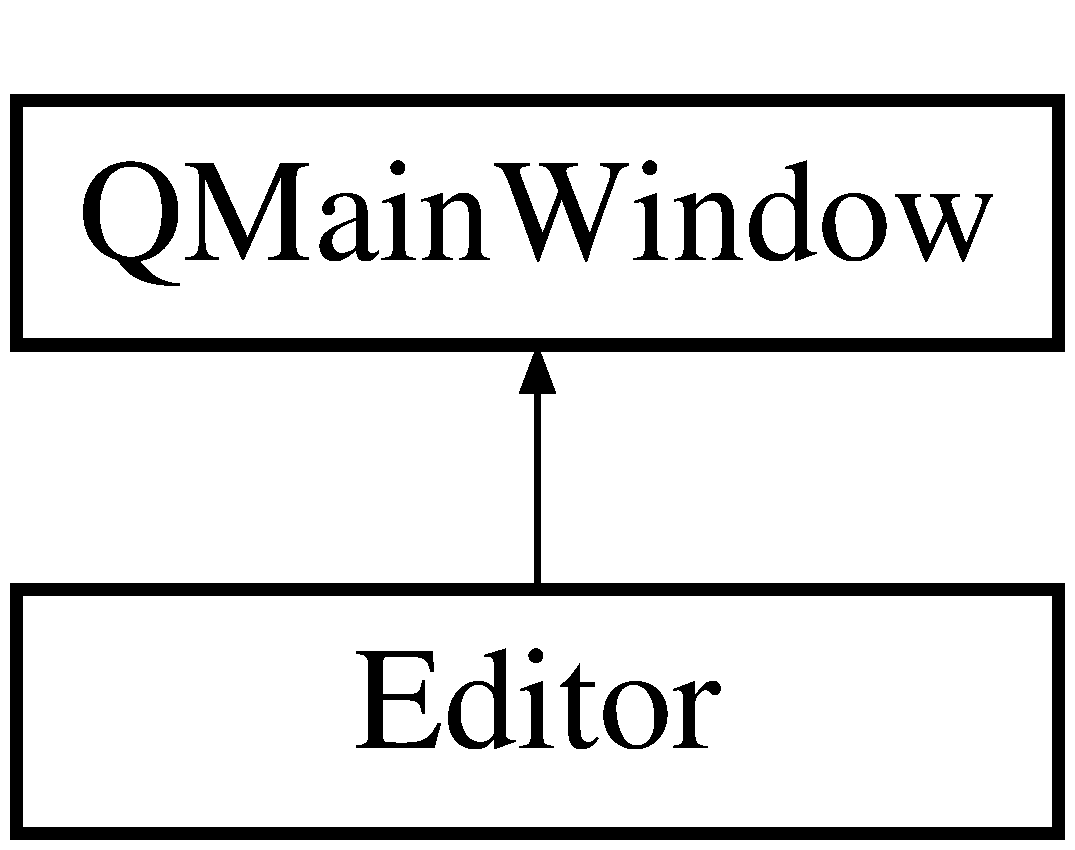
\includegraphics[height=2.000000cm]{class_editor}
\end{center}
\end{figure}
\subsection*{Métodos públicos}
\begin{DoxyCompactItemize}
\item 
\hypertarget{class_editor_a2918aceeffbc123a96e201b0934b9b16}{{\bfseries Editor} (Q\-Widget $\ast$parent=0)}\label{class_editor_a2918aceeffbc123a96e201b0934b9b16}

\end{DoxyCompactItemize}


La documentación para esta clase fue generada a partir de los siguientes ficheros\-:\begin{DoxyCompactItemize}
\item 
Editor/editor.\-h\item 
Editor/editor.\-cpp\end{DoxyCompactItemize}

\hypertarget{class_entrada_simbolo}{\section{Referencia de la Clase Entrada\-Simbolo}
\label{class_entrada_simbolo}\index{Entrada\-Simbolo@{Entrada\-Simbolo}}
}


La documentación para esta clase fue generada a partir de los siguientes ficheros\-:\begin{DoxyCompactItemize}
\item 
Programa/Entrada\-Simbolo.\-h\item 
Programa/Entrada\-Simbolo.\-cpp\end{DoxyCompactItemize}

\hypertarget{class_excepcion_legus}{\section{Referencia de la Clase Excepcion\-Legus}
\label{class_excepcion_legus}\index{Excepcion\-Legus@{Excepcion\-Legus}}
}
\subsection*{Métodos públicos}
\begin{DoxyCompactItemize}
\item 
\hypertarget{class_excepcion_legus_adba881013d63c418e3b5e7de3983d727}{{\bfseries Excepcion\-Legus} (const string \&mensaje)}\label{class_excepcion_legus_adba881013d63c418e3b5e7de3983d727}

\item 
\hypertarget{class_excepcion_legus_aa69a16fe17200a2944c3d1b78a3b8e6e}{{\bfseries Excepcion\-Legus} (const string \&mensaje, const int numero\-De\-Linea)}\label{class_excepcion_legus_aa69a16fe17200a2944c3d1b78a3b8e6e}

\item 
\hypertarget{class_excepcion_legus_ae7f5108035e64b28a4ad41944be04b6a}{string {\bfseries obtener\-Mensaje} ()}\label{class_excepcion_legus_ae7f5108035e64b28a4ad41944be04b6a}

\item 
\hypertarget{class_excepcion_legus_a388b5c30962877f7d5115111d08d1429}{int {\bfseries obtener\-Numero\-De\-Linea} ()}\label{class_excepcion_legus_a388b5c30962877f7d5115111d08d1429}

\end{DoxyCompactItemize}


La documentación para esta clase fue generada a partir de los siguientes ficheros\-:\begin{DoxyCompactItemize}
\item 
Programa/Excepcion\-Legus.\-h\item 
Programa/Excepcion\-Legus.\-cpp\end{DoxyCompactItemize}

\hypertarget{class_expresion}{\section{Referencia de la Clase Expresion}
\label{class_expresion}\index{Expresion@{Expresion}}
}
Diagrama de herencias de Expresion\begin{figure}[H]
\begin{center}
\leavevmode
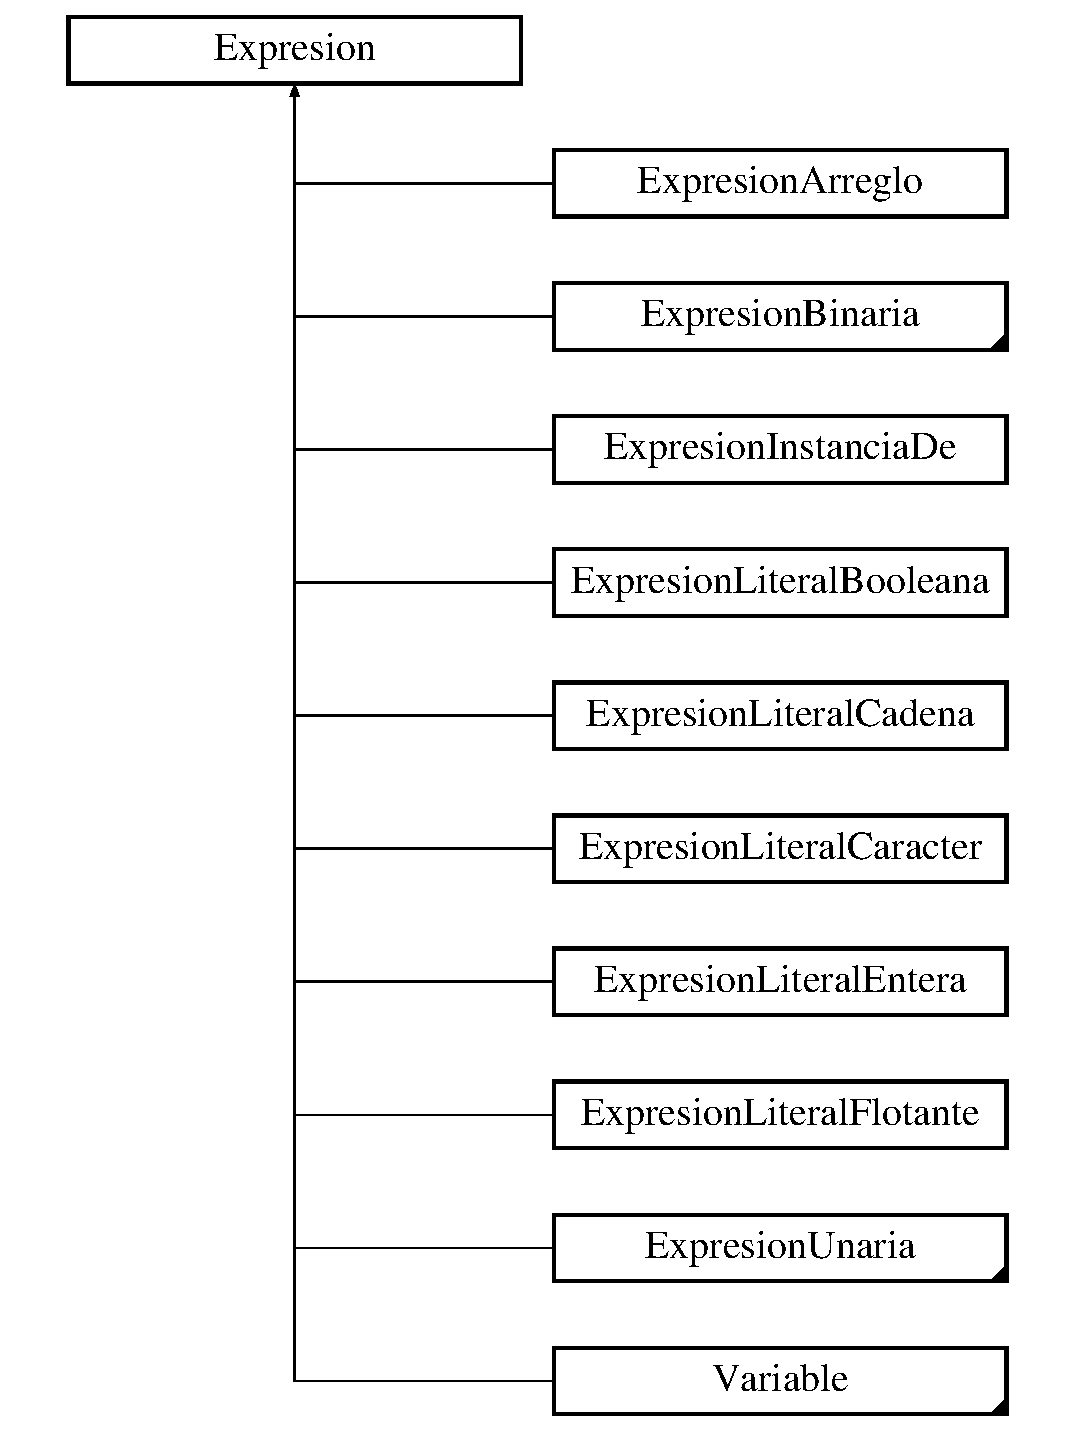
\includegraphics[height=11.000000cm]{class_expresion}
\end{center}
\end{figure}
\subsection*{Métodos públicos}
\begin{DoxyCompactItemize}
\item 
\hypertarget{class_expresion_a47f537b0bfb42f87df3130fe00eb417a}{{\bfseries Expresion} (Expresiones tipo, int numero\-De\-Linea)}\label{class_expresion_a47f537b0bfb42f87df3130fe00eb417a}

\item 
\hypertarget{class_expresion_ab28509da9a3eb68ae5a316484ac6f94a}{virtual \hyperlink{class_tipo}{Tipo} $\ast$ {\bfseries validar\-Semantica} ()=0}\label{class_expresion_ab28509da9a3eb68ae5a316484ac6f94a}

\item 
\hypertarget{class_expresion_afe2ed369d6f74507dfa46e4725dbb088}{virtual string {\bfseries generar\-Codigo\-Java} ()=0}\label{class_expresion_afe2ed369d6f74507dfa46e4725dbb088}

\end{DoxyCompactItemize}
\subsection*{Atributos públicos}
\begin{DoxyCompactItemize}
\item 
\hypertarget{class_expresion_a8653f08a895f21b44705a58f4d509a0f}{Expresiones {\bfseries tipo}}\label{class_expresion_a8653f08a895f21b44705a58f4d509a0f}

\item 
\hypertarget{class_expresion_a10c92265778cc9dd340de83cbf6cff02}{\hyperlink{class_tipo}{Tipo} $\ast$ {\bfseries tipo\-Inferido}}\label{class_expresion_a10c92265778cc9dd340de83cbf6cff02}

\item 
\hypertarget{class_expresion_a802df024cdb46c84d5404d32da40ead1}{int {\bfseries numero\-De\-Linea}}\label{class_expresion_a802df024cdb46c84d5404d32da40ead1}

\end{DoxyCompactItemize}


La documentación para esta clase fue generada a partir de los siguientes ficheros\-:\begin{DoxyCompactItemize}
\item 
Expresion/Expresion.\-h\item 
Expresion/Expresion.\-cpp\end{DoxyCompactItemize}

\hypertarget{class_expresion_arreglo}{\section{Referencia de la Clase Expresion\-Arreglo}
\label{class_expresion_arreglo}\index{Expresion\-Arreglo@{Expresion\-Arreglo}}
}
Diagrama de herencias de Expresion\-Arreglo\begin{figure}[H]
\begin{center}
\leavevmode
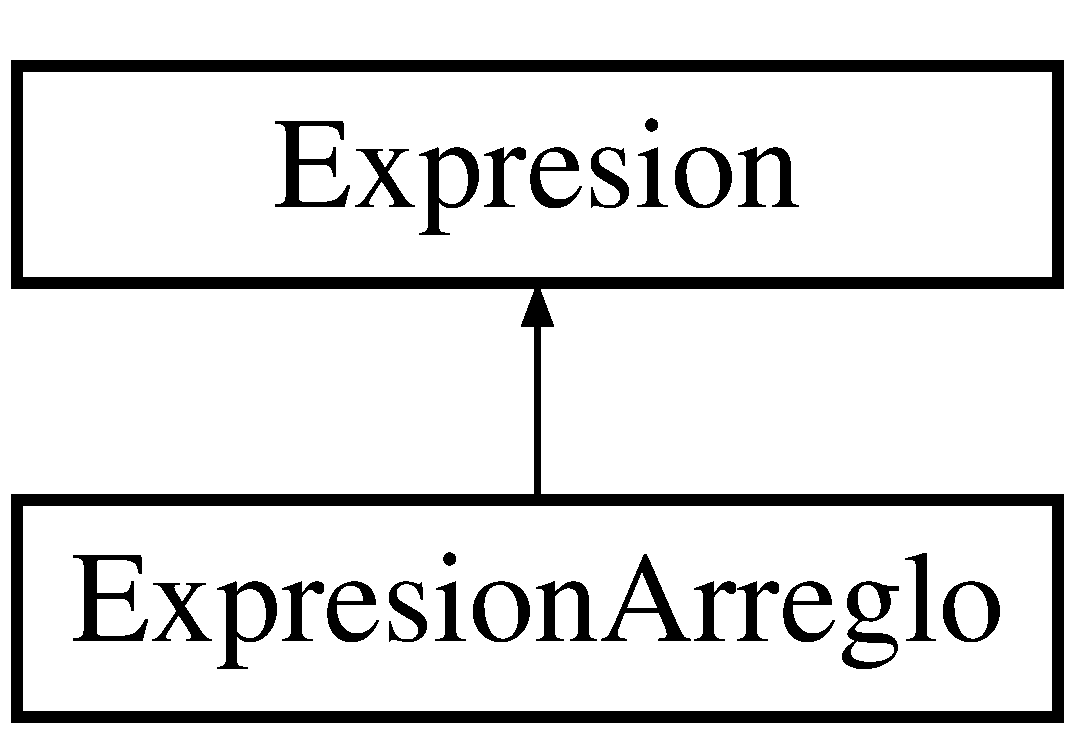
\includegraphics[height=2.000000cm]{class_expresion_arreglo}
\end{center}
\end{figure}
\subsection*{Métodos públicos}
\begin{DoxyCompactItemize}
\item 
\hypertarget{class_expresion_arreglo_a2713349df69f609421bb9fc363827d34}{{\bfseries Expresion\-Arreglo} (int numero\-De\-Linea)}\label{class_expresion_arreglo_a2713349df69f609421bb9fc363827d34}

\item 
\hypertarget{class_expresion_arreglo_aef6f63ff7e04452693c2a3dcb403d0af}{virtual \hyperlink{class_tipo}{Tipo} $\ast$ {\bfseries validar\-Semantica} ()}\label{class_expresion_arreglo_aef6f63ff7e04452693c2a3dcb403d0af}

\item 
\hypertarget{class_expresion_arreglo_a51ad1867ddbd683a3926583788b8075d}{virtual string {\bfseries generar\-Codigo\-Java} ()}\label{class_expresion_arreglo_a51ad1867ddbd683a3926583788b8075d}

\end{DoxyCompactItemize}
\subsection*{Otros miembros heredados}


La documentación para esta clase fue generada a partir de los siguientes ficheros\-:\begin{DoxyCompactItemize}
\item 
Expresion\-Arreglo.\-h\item 
Expresion\-Arreglo.\-cpp\end{DoxyCompactItemize}

\hypertarget{class_expresion_binaria}{\section{Referencia de la Clase Expresion\-Binaria}
\label{class_expresion_binaria}\index{Expresion\-Binaria@{Expresion\-Binaria}}
}
Diagrama de herencias de Expresion\-Binaria\begin{figure}[H]
\begin{center}
\leavevmode
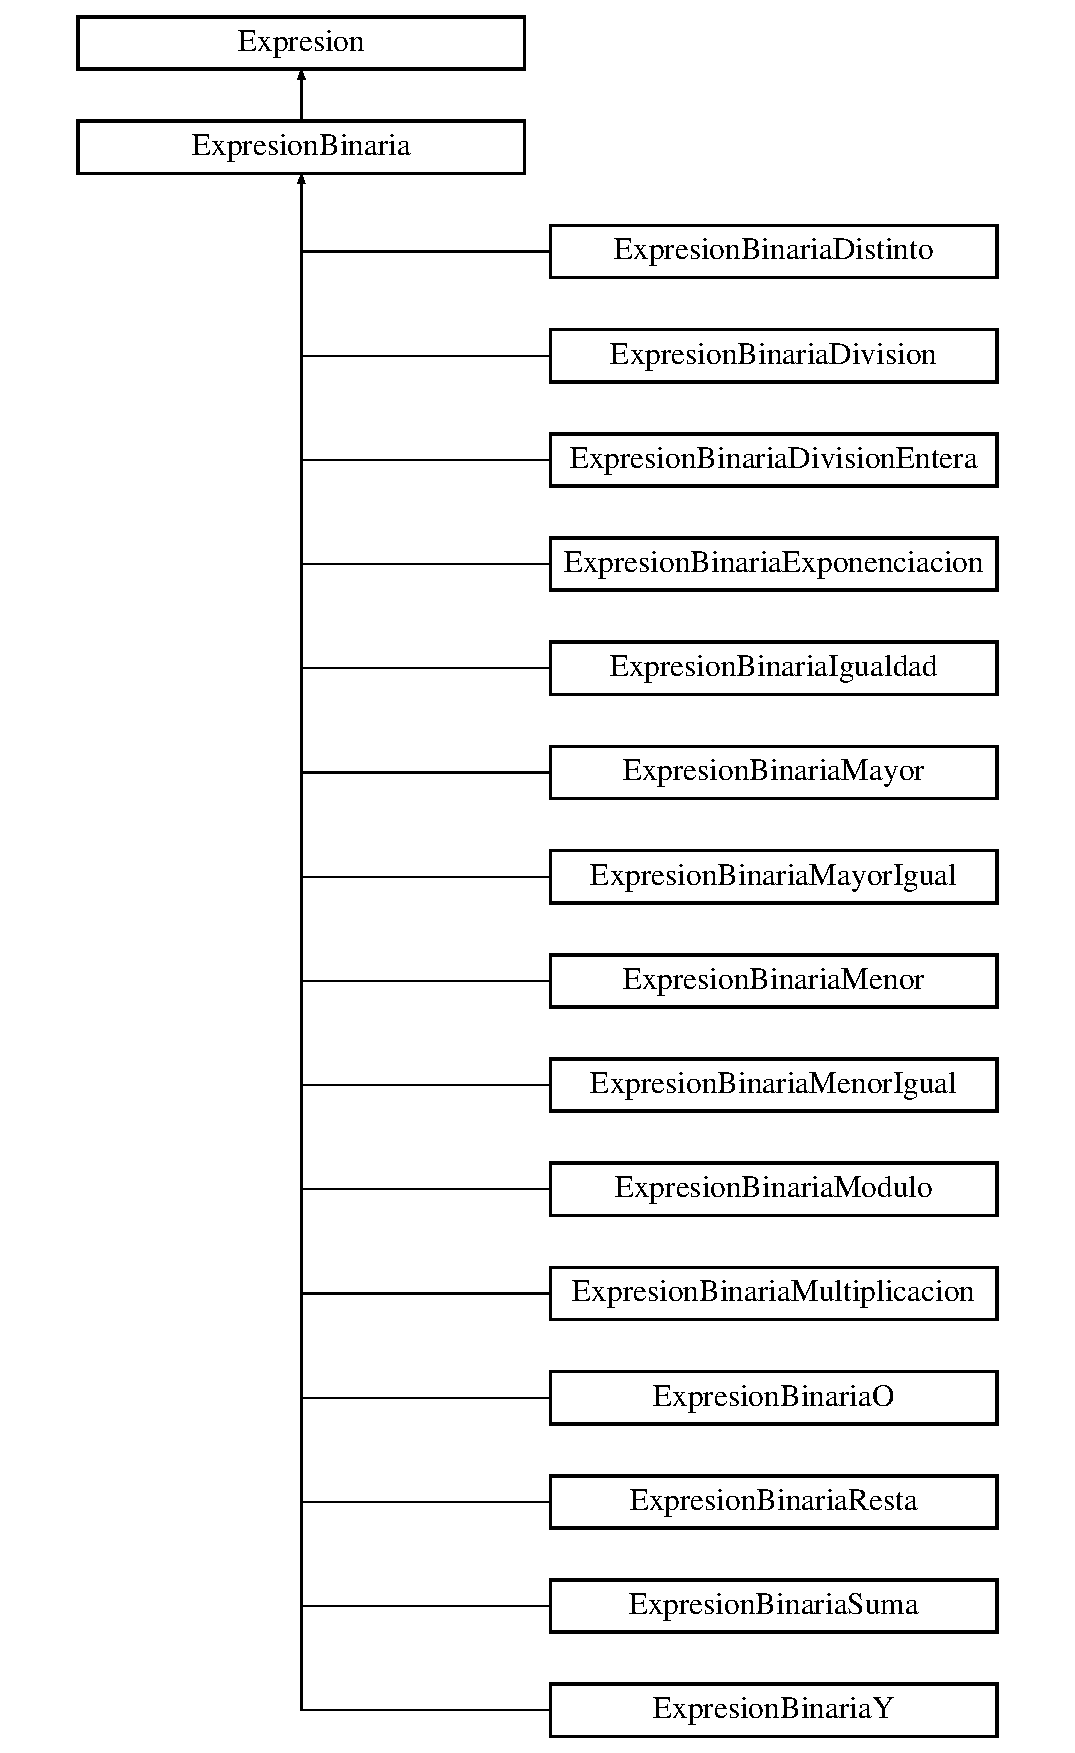
\includegraphics[height=12.000000cm]{class_expresion_binaria}
\end{center}
\end{figure}
\subsection*{Métodos públicos}
\begin{DoxyCompactItemize}
\item 
\hypertarget{class_expresion_binaria_a91e06b6736e260ce0c00f3ef1f007ff9}{{\bfseries Expresion\-Binaria} (\hyperlink{class_expresion}{Expresion} $\ast$izquierda, \hyperlink{class_expresion}{Expresion} $\ast$derecha, Expresiones tipo, int numero\-De\-Linea)}\label{class_expresion_binaria_a91e06b6736e260ce0c00f3ef1f007ff9}

\item 
\hypertarget{class_expresion_binaria_aff551bc7f050adefd3a4724c85de8294}{\hyperlink{class_expresion}{Expresion} $\ast$ {\bfseries obtener\-Expresion\-Izquierda} ()}\label{class_expresion_binaria_aff551bc7f050adefd3a4724c85de8294}

\item 
\hypertarget{class_expresion_binaria_a0eeed2c5ffaaa644fe13a194ff5b79e4}{\hyperlink{class_expresion}{Expresion} $\ast$ {\bfseries obtener\-Expresion\-Derecha} ()}\label{class_expresion_binaria_a0eeed2c5ffaaa644fe13a194ff5b79e4}

\end{DoxyCompactItemize}
\subsection*{Otros miembros heredados}


La documentación para esta clase fue generada a partir de los siguientes ficheros\-:\begin{DoxyCompactItemize}
\item 
Expresion/\-Expresion\-Binaria/Expresion\-Binaria.\-h\item 
Expresion/\-Expresion\-Binaria/Expresion\-Binaria.\-cpp\end{DoxyCompactItemize}

\hypertarget{class_expresion_binaria_distinto}{\section{Referencia de la Clase Expresion\-Binaria\-Distinto}
\label{class_expresion_binaria_distinto}\index{Expresion\-Binaria\-Distinto@{Expresion\-Binaria\-Distinto}}
}
Diagrama de herencias de Expresion\-Binaria\-Distinto\begin{figure}[H]
\begin{center}
\leavevmode
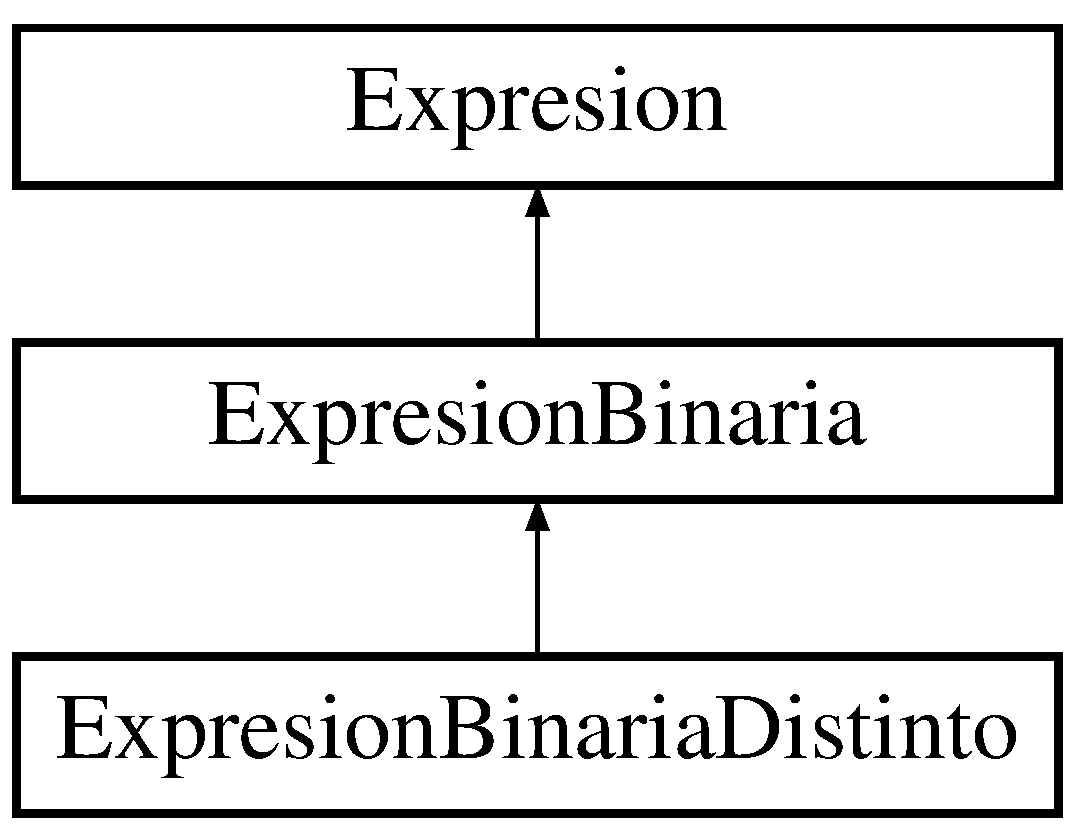
\includegraphics[height=3.000000cm]{class_expresion_binaria_distinto}
\end{center}
\end{figure}
\subsection*{Métodos públicos}
\begin{DoxyCompactItemize}
\item 
\hypertarget{class_expresion_binaria_distinto_a8f5d4b08dbf4eac2899d1e44e175b16c}{{\bfseries Expresion\-Binaria\-Distinto} (\hyperlink{class_expresion}{Expresion} $\ast$izquierda, \hyperlink{class_expresion}{Expresion} $\ast$derecha, int numero\-De\-Linea)}\label{class_expresion_binaria_distinto_a8f5d4b08dbf4eac2899d1e44e175b16c}

\item 
\hypertarget{class_expresion_binaria_distinto_ad1df37ee5fadedf3105b28cab2ef6486}{virtual \hyperlink{class_tipo}{Tipo} $\ast$ {\bfseries validar\-Semantica} ()}\label{class_expresion_binaria_distinto_ad1df37ee5fadedf3105b28cab2ef6486}

\item 
\hypertarget{class_expresion_binaria_distinto_a615a1cebbf16554ccc7c4b874a31a6f7}{virtual string {\bfseries generar\-Codigo\-Java} ()}\label{class_expresion_binaria_distinto_a615a1cebbf16554ccc7c4b874a31a6f7}

\end{DoxyCompactItemize}
\subsection*{Otros miembros heredados}


La documentación para esta clase fue generada a partir de los siguientes ficheros\-:\begin{DoxyCompactItemize}
\item 
Expresion/\-Expresion\-Binaria/Expresion\-Binaria\-Distinto.\-h\item 
Expresion/\-Expresion\-Binaria/Expresion\-Binaria\-Distinto.\-cpp\end{DoxyCompactItemize}

\hypertarget{class_expresion_binaria_division}{\section{Referencia de la Clase Expresion\-Binaria\-Division}
\label{class_expresion_binaria_division}\index{Expresion\-Binaria\-Division@{Expresion\-Binaria\-Division}}
}
Diagrama de herencias de Expresion\-Binaria\-Division\begin{figure}[H]
\begin{center}
\leavevmode
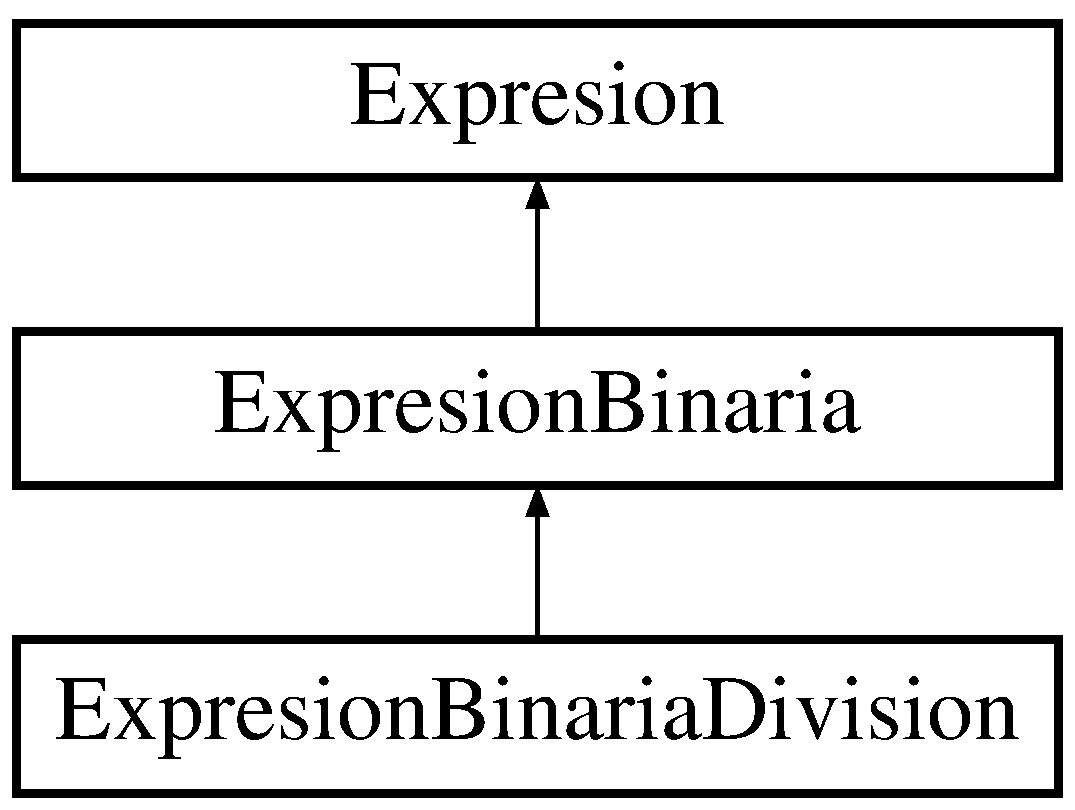
\includegraphics[height=3.000000cm]{class_expresion_binaria_division}
\end{center}
\end{figure}
\subsection*{Métodos públicos}
\begin{DoxyCompactItemize}
\item 
\hypertarget{class_expresion_binaria_division_afe1810c85fd586bfc76abdbc77332129}{{\bfseries Expresion\-Binaria\-Division} (\hyperlink{class_expresion}{Expresion} $\ast$izquierda, \hyperlink{class_expresion}{Expresion} $\ast$derecha, int numero\-De\-Linea)}\label{class_expresion_binaria_division_afe1810c85fd586bfc76abdbc77332129}

\item 
\hypertarget{class_expresion_binaria_division_aee97ebfc28e0fe9d7336b9ad4cc3343b}{virtual \hyperlink{class_tipo}{Tipo} $\ast$ {\bfseries validar\-Semantica} ()}\label{class_expresion_binaria_division_aee97ebfc28e0fe9d7336b9ad4cc3343b}

\item 
\hypertarget{class_expresion_binaria_division_a3d70135392ad0a69b898a654a8c6eba7}{virtual string {\bfseries generar\-Codigo\-Java} ()}\label{class_expresion_binaria_division_a3d70135392ad0a69b898a654a8c6eba7}

\end{DoxyCompactItemize}
\subsection*{Otros miembros heredados}


La documentación para esta clase fue generada a partir de los siguientes ficheros\-:\begin{DoxyCompactItemize}
\item 
Expresion/\-Expresion\-Binaria/Expresion\-Binaria\-Division.\-h\item 
Expresion/\-Expresion\-Binaria/Expresion\-Binaria\-Division.\-cpp\end{DoxyCompactItemize}

\hypertarget{class_expresion_binaria_division_entera}{\section{Referencia de la Clase Expresion\-Binaria\-Division\-Entera}
\label{class_expresion_binaria_division_entera}\index{Expresion\-Binaria\-Division\-Entera@{Expresion\-Binaria\-Division\-Entera}}
}
Diagrama de herencias de Expresion\-Binaria\-Division\-Entera\begin{figure}[H]
\begin{center}
\leavevmode
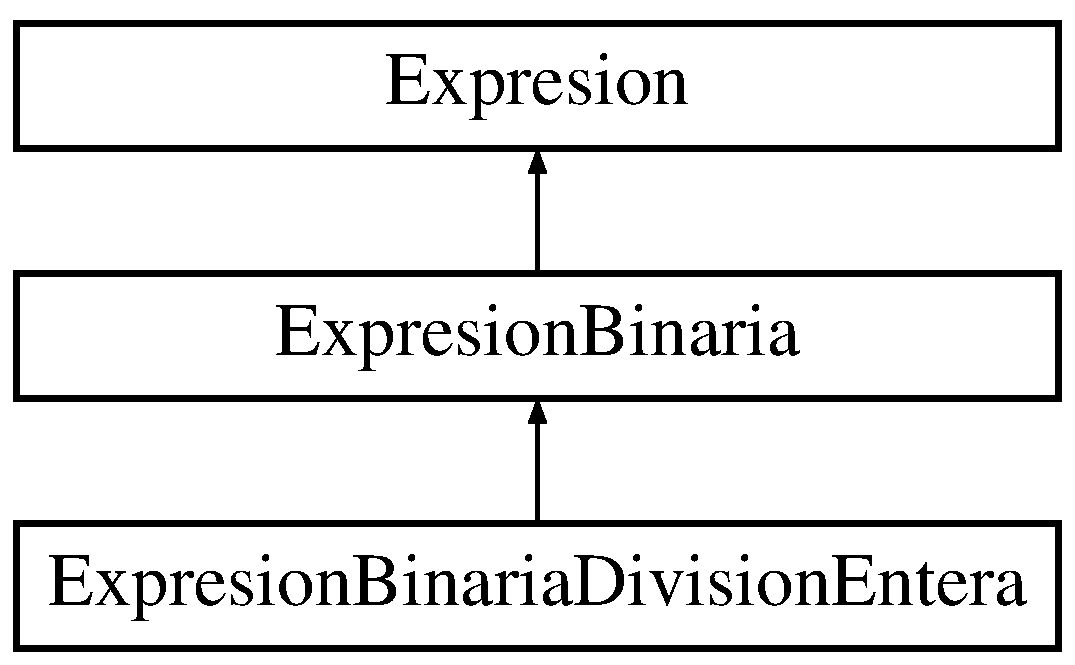
\includegraphics[height=3.000000cm]{class_expresion_binaria_division_entera}
\end{center}
\end{figure}
\subsection*{Métodos públicos}
\begin{DoxyCompactItemize}
\item 
\hypertarget{class_expresion_binaria_division_entera_abfa494a119bf9bcedff18ae5a7728e12}{{\bfseries Expresion\-Binaria\-Division\-Entera} (\hyperlink{class_expresion}{Expresion} $\ast$izquierda, \hyperlink{class_expresion}{Expresion} $\ast$derecha, int numero\-De\-Linea)}\label{class_expresion_binaria_division_entera_abfa494a119bf9bcedff18ae5a7728e12}

\item 
\hypertarget{class_expresion_binaria_division_entera_a9c7ca80abec8d851fb71e0e6af0fc116}{virtual \hyperlink{class_tipo}{Tipo} $\ast$ {\bfseries validar\-Semantica} ()}\label{class_expresion_binaria_division_entera_a9c7ca80abec8d851fb71e0e6af0fc116}

\item 
\hypertarget{class_expresion_binaria_division_entera_acb72c82d5c5b95a84d71573970b3c0b0}{virtual string {\bfseries generar\-Codigo\-Java} ()}\label{class_expresion_binaria_division_entera_acb72c82d5c5b95a84d71573970b3c0b0}

\end{DoxyCompactItemize}
\subsection*{Otros miembros heredados}


La documentación para esta clase fue generada a partir de los siguientes ficheros\-:\begin{DoxyCompactItemize}
\item 
Expresion/\-Expresion\-Binaria/Expresion\-Binaria\-Division\-Entera.\-h\item 
Expresion/\-Expresion\-Binaria/Expresion\-Binaria\-Division\-Entera.\-cpp\end{DoxyCompactItemize}

\hypertarget{class_expresion_binaria_exponenciacion}{\section{Referencia de la Clase Expresion\-Binaria\-Exponenciacion}
\label{class_expresion_binaria_exponenciacion}\index{Expresion\-Binaria\-Exponenciacion@{Expresion\-Binaria\-Exponenciacion}}
}
Diagrama de herencias de Expresion\-Binaria\-Exponenciacion\begin{figure}[H]
\begin{center}
\leavevmode
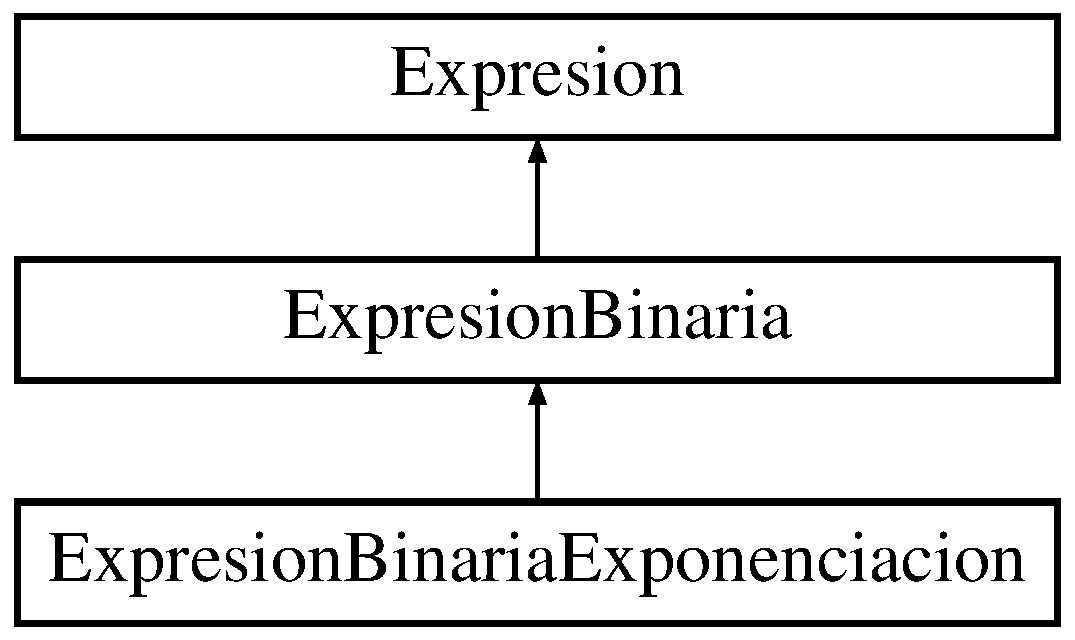
\includegraphics[height=3.000000cm]{class_expresion_binaria_exponenciacion}
\end{center}
\end{figure}
\subsection*{Métodos públicos}
\begin{DoxyCompactItemize}
\item 
\hypertarget{class_expresion_binaria_exponenciacion_a3af0b11cfe4d11d53bd84eb1961854d0}{{\bfseries Expresion\-Binaria\-Exponenciacion} (\hyperlink{class_expresion}{Expresion} $\ast$izquierda, \hyperlink{class_expresion}{Expresion} $\ast$derecha, int numero\-De\-Linea)}\label{class_expresion_binaria_exponenciacion_a3af0b11cfe4d11d53bd84eb1961854d0}

\item 
\hypertarget{class_expresion_binaria_exponenciacion_aad6651ca6c4b4013d8b3d2fe0be400ef}{virtual \hyperlink{class_tipo}{Tipo} $\ast$ {\bfseries validar\-Semantica} ()}\label{class_expresion_binaria_exponenciacion_aad6651ca6c4b4013d8b3d2fe0be400ef}

\item 
\hypertarget{class_expresion_binaria_exponenciacion_a34b82f5b0b312949d02c010fdd13cd5c}{virtual string {\bfseries generar\-Codigo\-Java} ()}\label{class_expresion_binaria_exponenciacion_a34b82f5b0b312949d02c010fdd13cd5c}

\end{DoxyCompactItemize}
\subsection*{Otros miembros heredados}


La documentación para esta clase fue generada a partir de los siguientes ficheros\-:\begin{DoxyCompactItemize}
\item 
Expresion/\-Expresion\-Binaria/Expresion\-Binaria\-Exponenciacion.\-h\item 
Expresion/\-Expresion\-Binaria/Expresion\-Binaria\-Exponenciacion.\-cpp\end{DoxyCompactItemize}

\hypertarget{class_expresion_binaria_igualdad}{\section{Referencia de la Clase Expresion\-Binaria\-Igualdad}
\label{class_expresion_binaria_igualdad}\index{Expresion\-Binaria\-Igualdad@{Expresion\-Binaria\-Igualdad}}
}
Diagrama de herencias de Expresion\-Binaria\-Igualdad\begin{figure}[H]
\begin{center}
\leavevmode
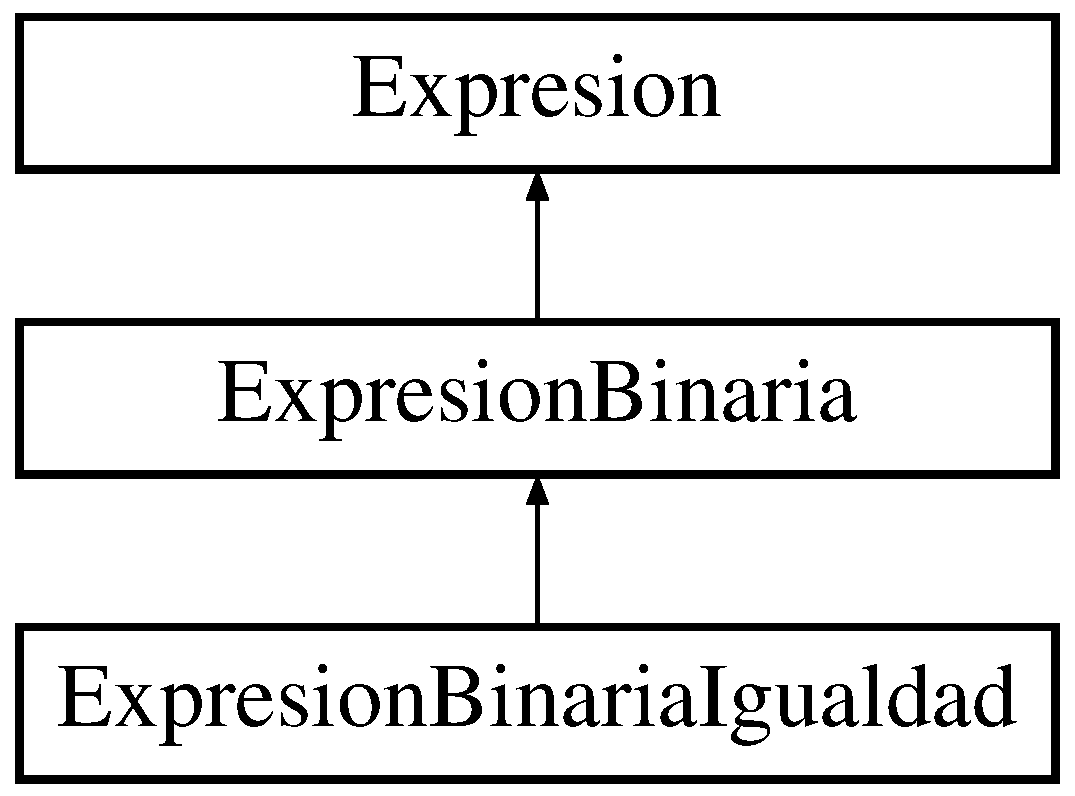
\includegraphics[height=3.000000cm]{class_expresion_binaria_igualdad}
\end{center}
\end{figure}
\subsection*{Métodos públicos}
\begin{DoxyCompactItemize}
\item 
\hypertarget{class_expresion_binaria_igualdad_adf79611697265d0ca2d0c52efcf187b9}{{\bfseries Expresion\-Binaria\-Igualdad} (\hyperlink{class_expresion}{Expresion} $\ast$izquierda, \hyperlink{class_expresion}{Expresion} $\ast$derecha, int numero\-De\-Linea)}\label{class_expresion_binaria_igualdad_adf79611697265d0ca2d0c52efcf187b9}

\item 
\hypertarget{class_expresion_binaria_igualdad_ae0d7151da1bf22098745fe207285deee}{virtual \hyperlink{class_tipo}{Tipo} $\ast$ {\bfseries validar\-Semantica} ()}\label{class_expresion_binaria_igualdad_ae0d7151da1bf22098745fe207285deee}

\item 
\hypertarget{class_expresion_binaria_igualdad_aed73c6d738fd0ff3cdb901eac690434c}{virtual string {\bfseries generar\-Codigo\-Java} ()}\label{class_expresion_binaria_igualdad_aed73c6d738fd0ff3cdb901eac690434c}

\end{DoxyCompactItemize}
\subsection*{Otros miembros heredados}


La documentación para esta clase fue generada a partir de los siguientes ficheros\-:\begin{DoxyCompactItemize}
\item 
Expresion/\-Expresion\-Binaria/Expresion\-Binaria\-Igualdad.\-h\item 
Expresion/\-Expresion\-Binaria/Expresion\-Binaria\-Igualdad.\-cpp\end{DoxyCompactItemize}

\hypertarget{class_expresion_binaria_mayor}{\section{Referencia de la Clase Expresion\-Binaria\-Mayor}
\label{class_expresion_binaria_mayor}\index{Expresion\-Binaria\-Mayor@{Expresion\-Binaria\-Mayor}}
}
Diagrama de herencias de Expresion\-Binaria\-Mayor\begin{figure}[H]
\begin{center}
\leavevmode
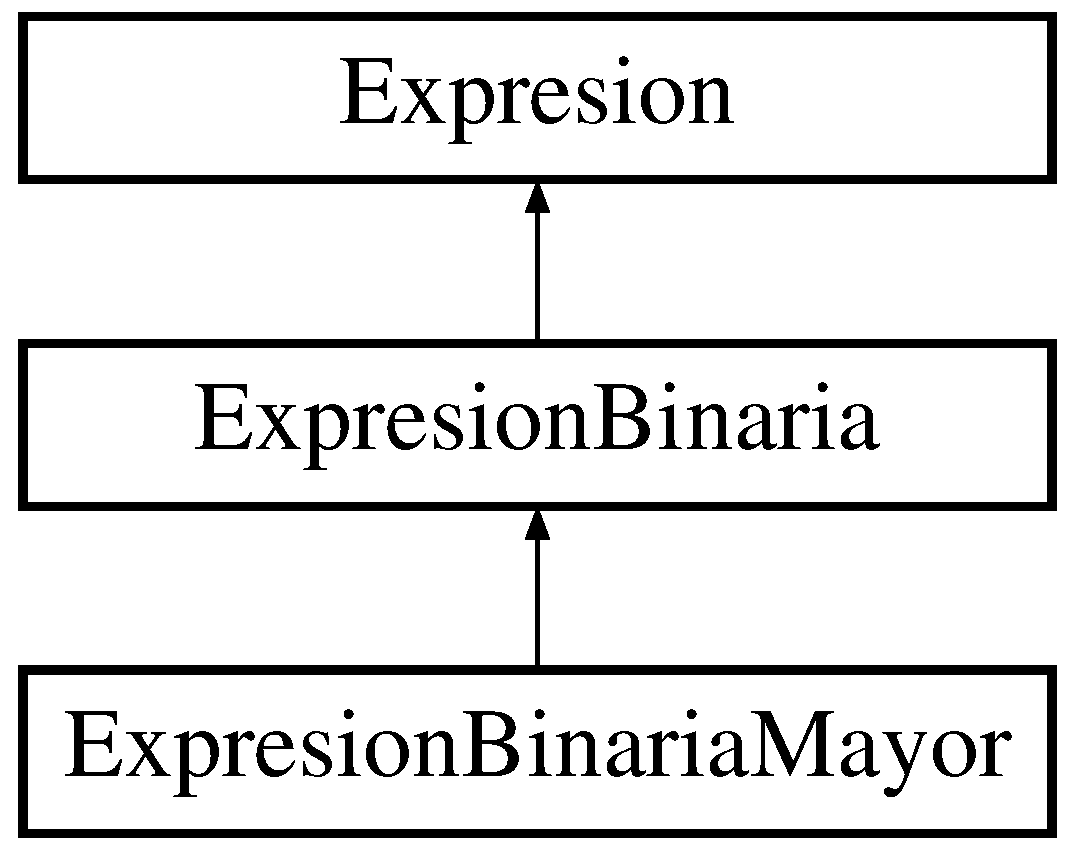
\includegraphics[height=3.000000cm]{class_expresion_binaria_mayor}
\end{center}
\end{figure}
\subsection*{Métodos públicos}
\begin{DoxyCompactItemize}
\item 
\hypertarget{class_expresion_binaria_mayor_acee27dbbe3bada9df7f94258f0f51b11}{{\bfseries Expresion\-Binaria\-Mayor} (\hyperlink{class_expresion}{Expresion} $\ast$izquierda, \hyperlink{class_expresion}{Expresion} $\ast$derecha, int numero\-De\-Linea)}\label{class_expresion_binaria_mayor_acee27dbbe3bada9df7f94258f0f51b11}

\item 
\hypertarget{class_expresion_binaria_mayor_a118356acb5b822ca9b19050550166f0e}{virtual \hyperlink{class_tipo}{Tipo} $\ast$ {\bfseries validar\-Semantica} ()}\label{class_expresion_binaria_mayor_a118356acb5b822ca9b19050550166f0e}

\item 
\hypertarget{class_expresion_binaria_mayor_aa60f0341ead7df4cdde8aaa534546892}{virtual string {\bfseries generar\-Codigo\-Java} ()}\label{class_expresion_binaria_mayor_aa60f0341ead7df4cdde8aaa534546892}

\end{DoxyCompactItemize}
\subsection*{Otros miembros heredados}


La documentación para esta clase fue generada a partir de los siguientes ficheros\-:\begin{DoxyCompactItemize}
\item 
Expresion/\-Expresion\-Binaria/Expresion\-Binaria\-Mayor.\-h\item 
Expresion/\-Expresion\-Binaria/Expresion\-Binaria\-Mayor.\-cpp\end{DoxyCompactItemize}

\hypertarget{class_expresion_binaria_mayor_igual}{\section{Referencia de la Clase Expresion\-Binaria\-Mayor\-Igual}
\label{class_expresion_binaria_mayor_igual}\index{Expresion\-Binaria\-Mayor\-Igual@{Expresion\-Binaria\-Mayor\-Igual}}
}
Diagrama de herencias de Expresion\-Binaria\-Mayor\-Igual\begin{figure}[H]
\begin{center}
\leavevmode
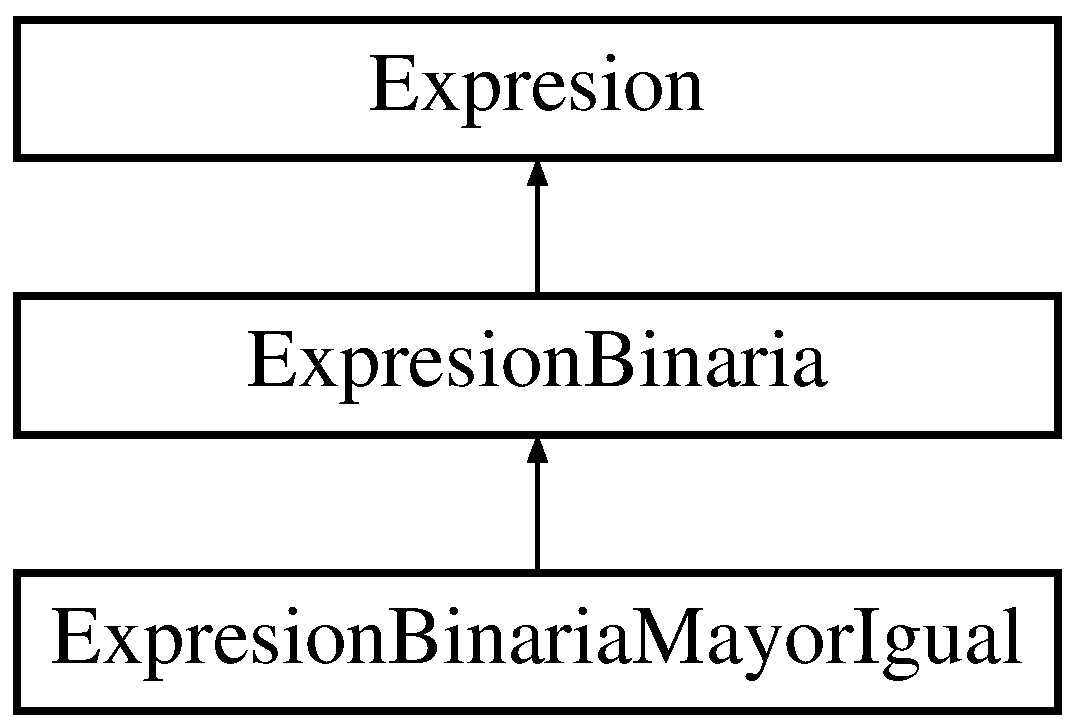
\includegraphics[height=3.000000cm]{class_expresion_binaria_mayor_igual}
\end{center}
\end{figure}
\subsection*{Métodos públicos}
\begin{DoxyCompactItemize}
\item 
\hypertarget{class_expresion_binaria_mayor_igual_abc403e915311ba1b100a4ac401c5daf2}{{\bfseries Expresion\-Binaria\-Mayor\-Igual} (\hyperlink{class_expresion}{Expresion} $\ast$izquierda, \hyperlink{class_expresion}{Expresion} $\ast$derecha, int numero\-De\-Linea)}\label{class_expresion_binaria_mayor_igual_abc403e915311ba1b100a4ac401c5daf2}

\item 
\hypertarget{class_expresion_binaria_mayor_igual_ae90f0ce32c6283eb1f112eb30390d755}{virtual \hyperlink{class_tipo}{Tipo} $\ast$ {\bfseries validar\-Semantica} ()}\label{class_expresion_binaria_mayor_igual_ae90f0ce32c6283eb1f112eb30390d755}

\item 
\hypertarget{class_expresion_binaria_mayor_igual_a6352bc5ca272bf89e4f166eb92d2af57}{virtual string {\bfseries generar\-Codigo\-Java} ()}\label{class_expresion_binaria_mayor_igual_a6352bc5ca272bf89e4f166eb92d2af57}

\end{DoxyCompactItemize}
\subsection*{Otros miembros heredados}


La documentación para esta clase fue generada a partir de los siguientes ficheros\-:\begin{DoxyCompactItemize}
\item 
Expresion/\-Expresion\-Binaria/Expresion\-Binaria\-Mayor\-Igual.\-h\item 
Expresion/\-Expresion\-Binaria/Expresion\-Binaria\-Mayor\-Igual.\-cpp\end{DoxyCompactItemize}

\hypertarget{class_expresion_binaria_menor}{\section{Referencia de la Clase Expresion\-Binaria\-Menor}
\label{class_expresion_binaria_menor}\index{Expresion\-Binaria\-Menor@{Expresion\-Binaria\-Menor}}
}
Diagrama de herencias de Expresion\-Binaria\-Menor\begin{figure}[H]
\begin{center}
\leavevmode
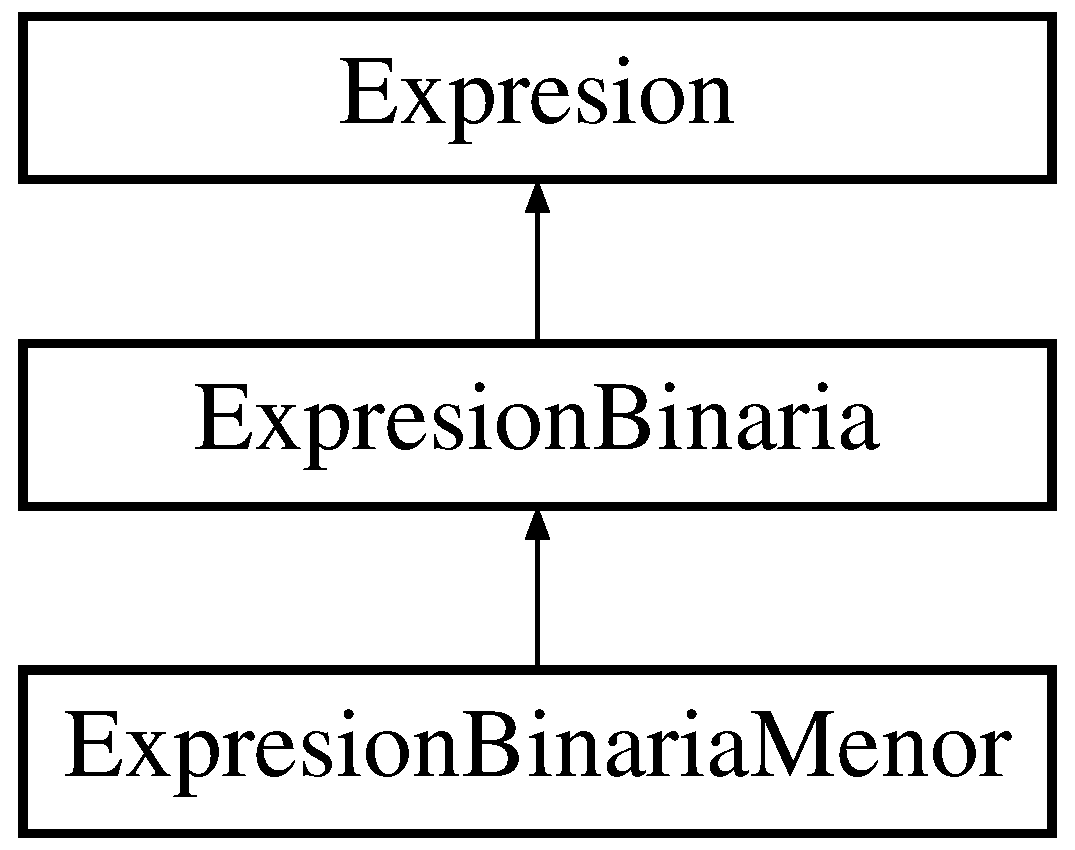
\includegraphics[height=3.000000cm]{class_expresion_binaria_menor}
\end{center}
\end{figure}
\subsection*{Métodos públicos}
\begin{DoxyCompactItemize}
\item 
\hypertarget{class_expresion_binaria_menor_aabf4f32a78741be4739f78ed10e82378}{{\bfseries Expresion\-Binaria\-Menor} (\hyperlink{class_expresion}{Expresion} $\ast$izquierda, \hyperlink{class_expresion}{Expresion} $\ast$derecha, int numero\-De\-Linea)}\label{class_expresion_binaria_menor_aabf4f32a78741be4739f78ed10e82378}

\item 
\hypertarget{class_expresion_binaria_menor_ac4062be428f8c03268aba3857099d5f5}{virtual \hyperlink{class_tipo}{Tipo} $\ast$ {\bfseries validar\-Semantica} ()}\label{class_expresion_binaria_menor_ac4062be428f8c03268aba3857099d5f5}

\item 
\hypertarget{class_expresion_binaria_menor_a86acaf9783a8735c35fc03d8a6eb064a}{virtual string {\bfseries generar\-Codigo\-Java} ()}\label{class_expresion_binaria_menor_a86acaf9783a8735c35fc03d8a6eb064a}

\end{DoxyCompactItemize}
\subsection*{Otros miembros heredados}


La documentación para esta clase fue generada a partir de los siguientes ficheros\-:\begin{DoxyCompactItemize}
\item 
Expresion/\-Expresion\-Binaria/Expresion\-Binaria\-Menor.\-h\item 
Expresion/\-Expresion\-Binaria/Expresion\-Binaria\-Menor.\-cpp\end{DoxyCompactItemize}

\hypertarget{class_expresion_binaria_menor_igual}{\section{Referencia de la Clase Expresion\-Binaria\-Menor\-Igual}
\label{class_expresion_binaria_menor_igual}\index{Expresion\-Binaria\-Menor\-Igual@{Expresion\-Binaria\-Menor\-Igual}}
}
Diagrama de herencias de Expresion\-Binaria\-Menor\-Igual\begin{figure}[H]
\begin{center}
\leavevmode
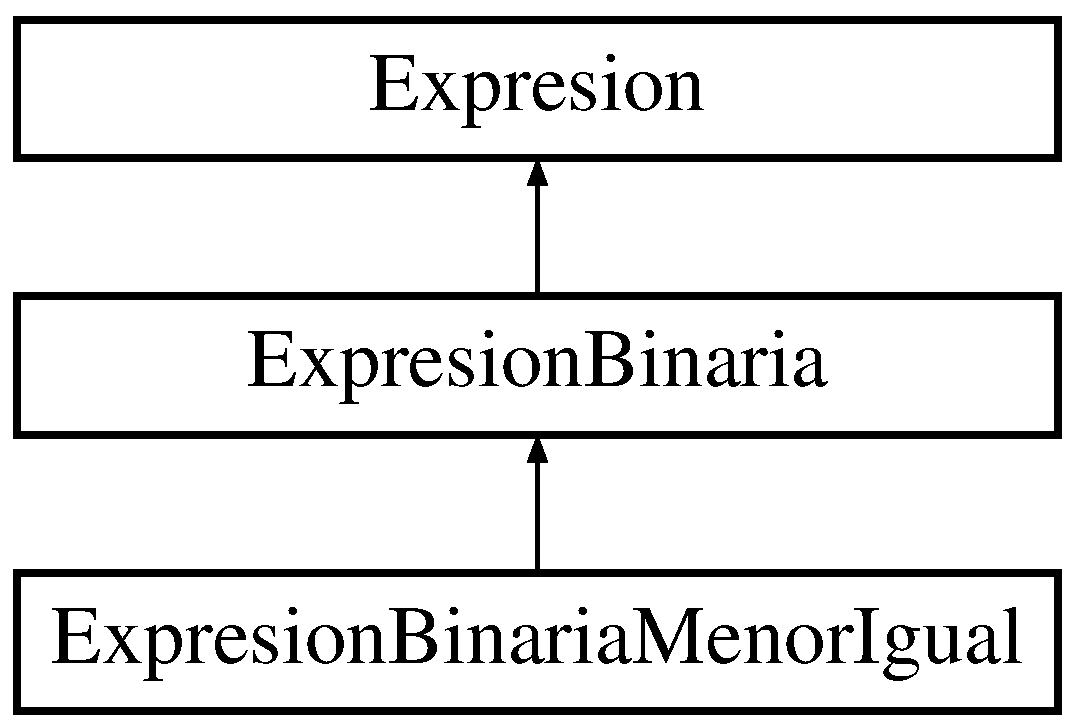
\includegraphics[height=3.000000cm]{class_expresion_binaria_menor_igual}
\end{center}
\end{figure}
\subsection*{Métodos públicos}
\begin{DoxyCompactItemize}
\item 
\hypertarget{class_expresion_binaria_menor_igual_a9ded70cedc472b5ef937015548bd89d7}{{\bfseries Expresion\-Binaria\-Menor\-Igual} (\hyperlink{class_expresion}{Expresion} $\ast$izquierda, \hyperlink{class_expresion}{Expresion} $\ast$derecha, int numero\-De\-Linea)}\label{class_expresion_binaria_menor_igual_a9ded70cedc472b5ef937015548bd89d7}

\item 
\hypertarget{class_expresion_binaria_menor_igual_af35c44bcf153a717ed899f82cfe16330}{virtual \hyperlink{class_tipo}{Tipo} $\ast$ {\bfseries validar\-Semantica} ()}\label{class_expresion_binaria_menor_igual_af35c44bcf153a717ed899f82cfe16330}

\item 
\hypertarget{class_expresion_binaria_menor_igual_a50bcd6f34a0c87c074d796bd9df3983a}{virtual string {\bfseries generar\-Codigo\-Java} ()}\label{class_expresion_binaria_menor_igual_a50bcd6f34a0c87c074d796bd9df3983a}

\end{DoxyCompactItemize}
\subsection*{Otros miembros heredados}


La documentación para esta clase fue generada a partir de los siguientes ficheros\-:\begin{DoxyCompactItemize}
\item 
Expresion/\-Expresion\-Binaria/Expresion\-Binaria\-Menor\-Igual.\-h\item 
Expresion/\-Expresion\-Binaria/Expresion\-Binaria\-Menor\-Igual.\-cpp\end{DoxyCompactItemize}

\hypertarget{class_expresion_binaria_modulo}{\section{Referencia de la Clase Expresion\-Binaria\-Modulo}
\label{class_expresion_binaria_modulo}\index{Expresion\-Binaria\-Modulo@{Expresion\-Binaria\-Modulo}}
}
Diagrama de herencias de Expresion\-Binaria\-Modulo\begin{figure}[H]
\begin{center}
\leavevmode
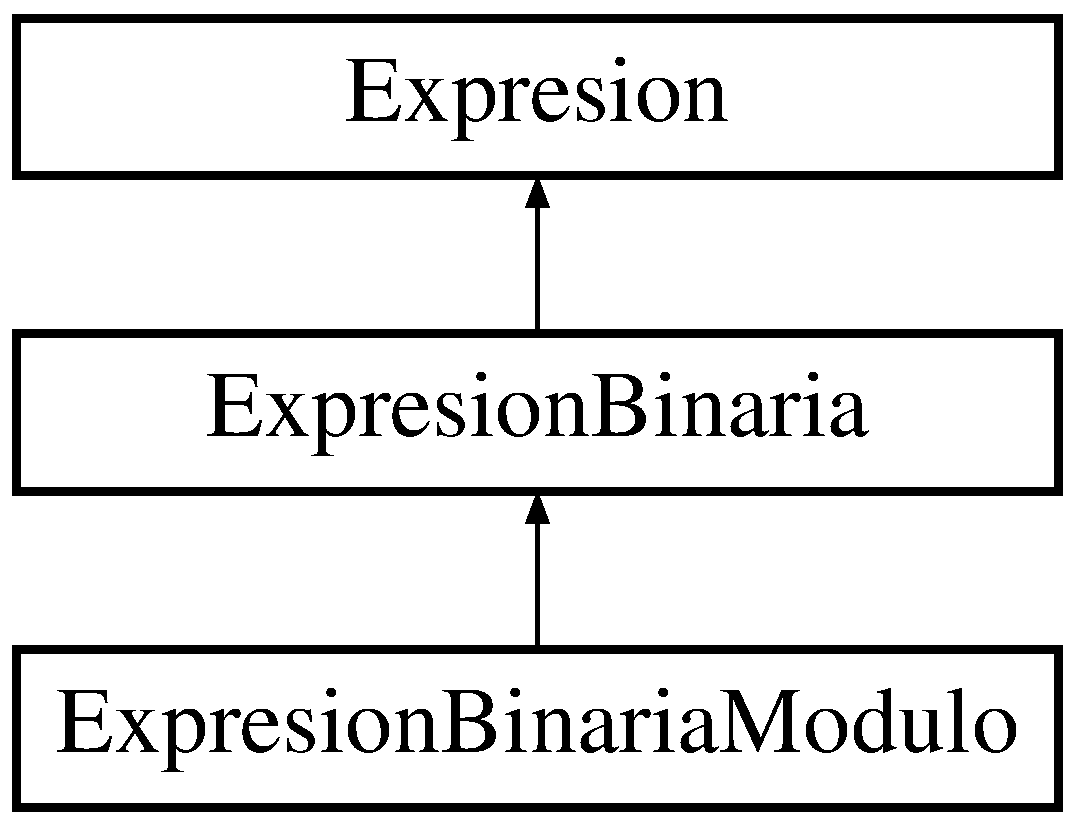
\includegraphics[height=3.000000cm]{class_expresion_binaria_modulo}
\end{center}
\end{figure}
\subsection*{Métodos públicos}
\begin{DoxyCompactItemize}
\item 
\hypertarget{class_expresion_binaria_modulo_a47dc7e956cf3e55393f0e8917ba11519}{{\bfseries Expresion\-Binaria\-Modulo} (\hyperlink{class_expresion}{Expresion} $\ast$izquierda, \hyperlink{class_expresion}{Expresion} $\ast$derecha, int numero\-De\-Linea)}\label{class_expresion_binaria_modulo_a47dc7e956cf3e55393f0e8917ba11519}

\item 
\hypertarget{class_expresion_binaria_modulo_acf7adb662d0193041e1d2f0c366070e4}{virtual \hyperlink{class_tipo}{Tipo} $\ast$ {\bfseries validar\-Semantica} ()}\label{class_expresion_binaria_modulo_acf7adb662d0193041e1d2f0c366070e4}

\item 
\hypertarget{class_expresion_binaria_modulo_ab28c33ff63bf04104c6e8208e2f624f9}{virtual string {\bfseries generar\-Codigo\-Java} ()}\label{class_expresion_binaria_modulo_ab28c33ff63bf04104c6e8208e2f624f9}

\end{DoxyCompactItemize}
\subsection*{Otros miembros heredados}


La documentación para esta clase fue generada a partir de los siguientes ficheros\-:\begin{DoxyCompactItemize}
\item 
Expresion/\-Expresion\-Binaria/Expresion\-Binaria\-Modulo.\-h\item 
Expresion/\-Expresion\-Binaria/Expresion\-Binaria\-Modulo.\-cpp\end{DoxyCompactItemize}

\hypertarget{class_expresion_binaria_multiplicacion}{\section{Referencia de la Clase Expresion\-Binaria\-Multiplicacion}
\label{class_expresion_binaria_multiplicacion}\index{Expresion\-Binaria\-Multiplicacion@{Expresion\-Binaria\-Multiplicacion}}
}
Diagrama de herencias de Expresion\-Binaria\-Multiplicacion\begin{figure}[H]
\begin{center}
\leavevmode
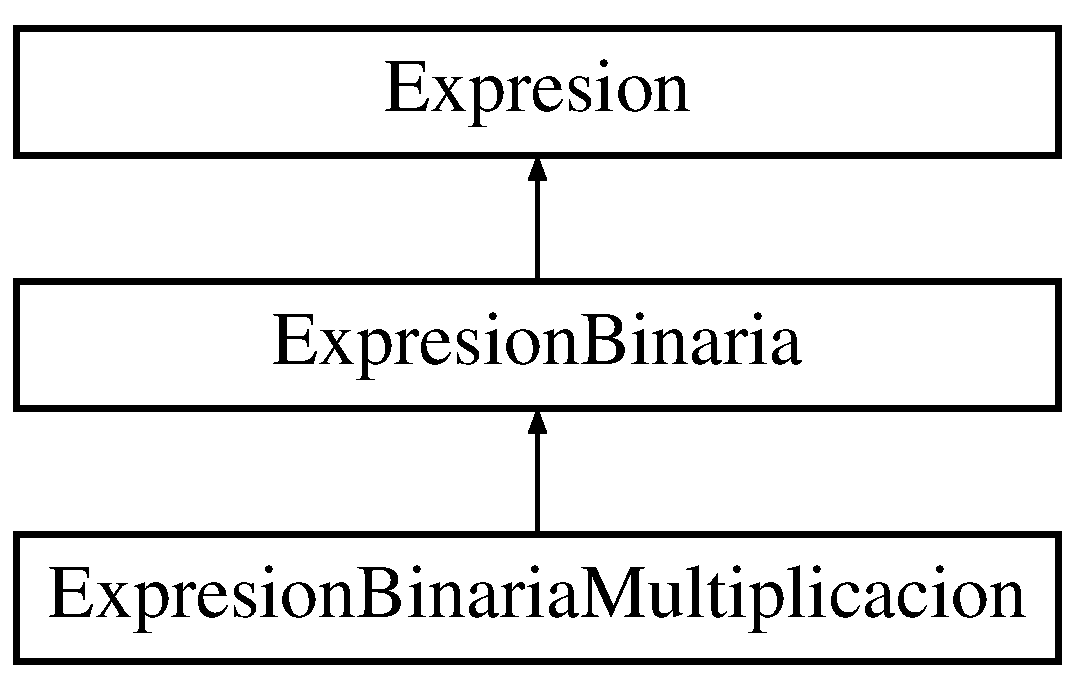
\includegraphics[height=3.000000cm]{class_expresion_binaria_multiplicacion}
\end{center}
\end{figure}
\subsection*{Métodos públicos}
\begin{DoxyCompactItemize}
\item 
\hypertarget{class_expresion_binaria_multiplicacion_ada46004d03bcf9818c0968b498f9f78b}{{\bfseries Expresion\-Binaria\-Multiplicacion} (\hyperlink{class_expresion}{Expresion} $\ast$izquierda, \hyperlink{class_expresion}{Expresion} $\ast$derecha, int numero\-De\-Linea)}\label{class_expresion_binaria_multiplicacion_ada46004d03bcf9818c0968b498f9f78b}

\item 
\hypertarget{class_expresion_binaria_multiplicacion_a15bcc9f381e17053afc4b77470581f6b}{virtual \hyperlink{class_tipo}{Tipo} $\ast$ {\bfseries validar\-Semantica} ()}\label{class_expresion_binaria_multiplicacion_a15bcc9f381e17053afc4b77470581f6b}

\item 
\hypertarget{class_expresion_binaria_multiplicacion_ab94f2121a01f41e924083666a75d3310}{virtual string {\bfseries generar\-Codigo\-Java} ()}\label{class_expresion_binaria_multiplicacion_ab94f2121a01f41e924083666a75d3310}

\end{DoxyCompactItemize}
\subsection*{Otros miembros heredados}


La documentación para esta clase fue generada a partir de los siguientes ficheros\-:\begin{DoxyCompactItemize}
\item 
Expresion/\-Expresion\-Binaria/Expresion\-Binaria\-Multiplicacion.\-h\item 
Expresion/\-Expresion\-Binaria/Expresion\-Binaria\-Multiplicacion.\-cpp\end{DoxyCompactItemize}

\hypertarget{class_expresion_binaria_o}{\section{Referencia de la Clase Expresion\-Binaria\-O}
\label{class_expresion_binaria_o}\index{Expresion\-Binaria\-O@{Expresion\-Binaria\-O}}
}
Diagrama de herencias de Expresion\-Binaria\-O\begin{figure}[H]
\begin{center}
\leavevmode
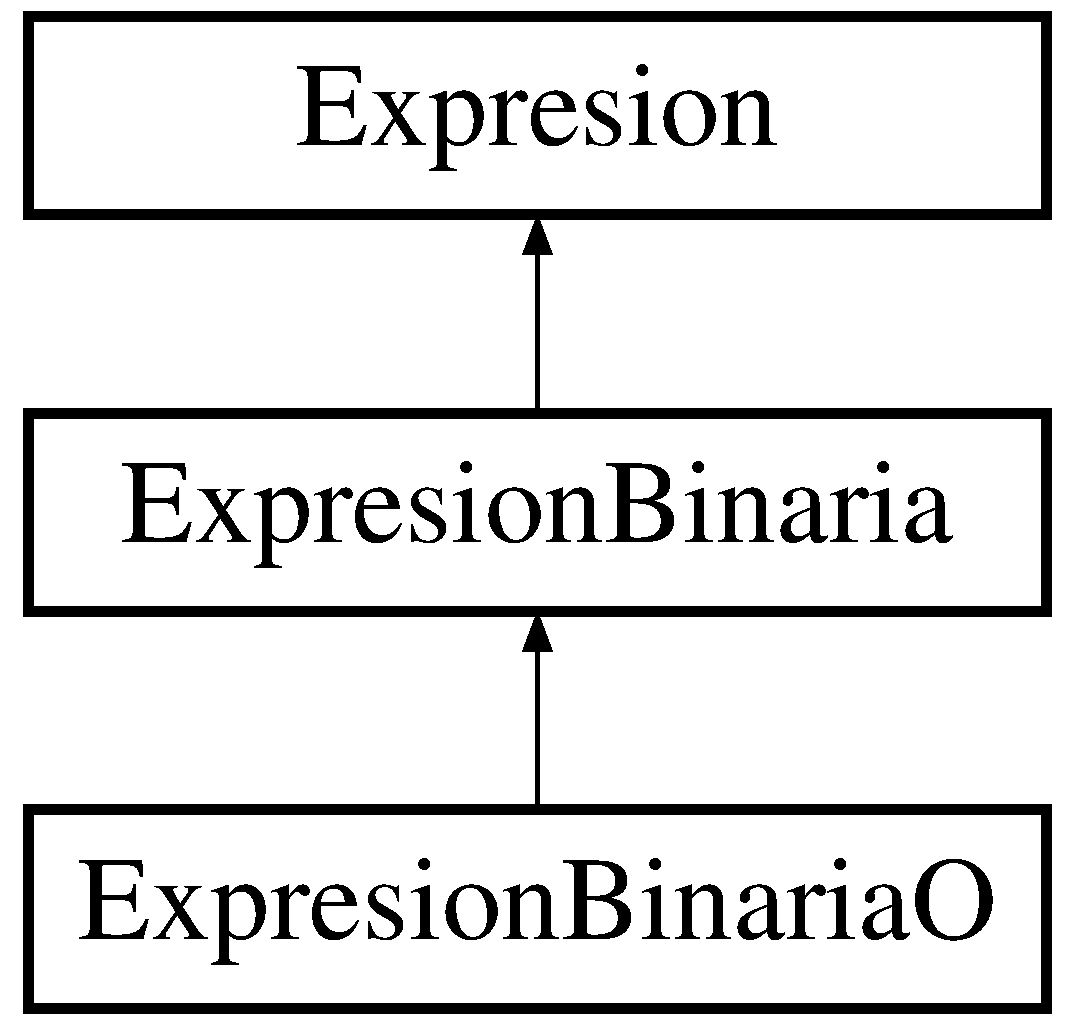
\includegraphics[height=3.000000cm]{class_expresion_binaria_o}
\end{center}
\end{figure}
\subsection*{Métodos públicos}
\begin{DoxyCompactItemize}
\item 
\hypertarget{class_expresion_binaria_o_a8b8be1b1e05c541961fc3d3acb1725d0}{{\bfseries Expresion\-Binaria\-O} (\hyperlink{class_expresion}{Expresion} $\ast$izquierda, \hyperlink{class_expresion}{Expresion} $\ast$derecha, int numero\-De\-Linea)}\label{class_expresion_binaria_o_a8b8be1b1e05c541961fc3d3acb1725d0}

\item 
\hypertarget{class_expresion_binaria_o_a604c2812bc9bec75fdf0396c6a261252}{virtual \hyperlink{class_tipo}{Tipo} $\ast$ {\bfseries validar\-Semantica} ()}\label{class_expresion_binaria_o_a604c2812bc9bec75fdf0396c6a261252}

\item 
\hypertarget{class_expresion_binaria_o_ae533c76a4744d62b90567c1fe61bed07}{virtual string {\bfseries generar\-Codigo\-Java} ()}\label{class_expresion_binaria_o_ae533c76a4744d62b90567c1fe61bed07}

\end{DoxyCompactItemize}
\subsection*{Otros miembros heredados}


La documentación para esta clase fue generada a partir de los siguientes ficheros\-:\begin{DoxyCompactItemize}
\item 
Expresion/\-Expresion\-Binaria/Expresion\-Binaria\-O.\-h\item 
Expresion/\-Expresion\-Binaria/Expresion\-Binaria\-O.\-cpp\end{DoxyCompactItemize}

\hypertarget{class_expresion_binaria_resta}{\section{Referencia de la Clase Expresion\-Binaria\-Resta}
\label{class_expresion_binaria_resta}\index{Expresion\-Binaria\-Resta@{Expresion\-Binaria\-Resta}}
}
Diagrama de herencias de Expresion\-Binaria\-Resta\begin{figure}[H]
\begin{center}
\leavevmode
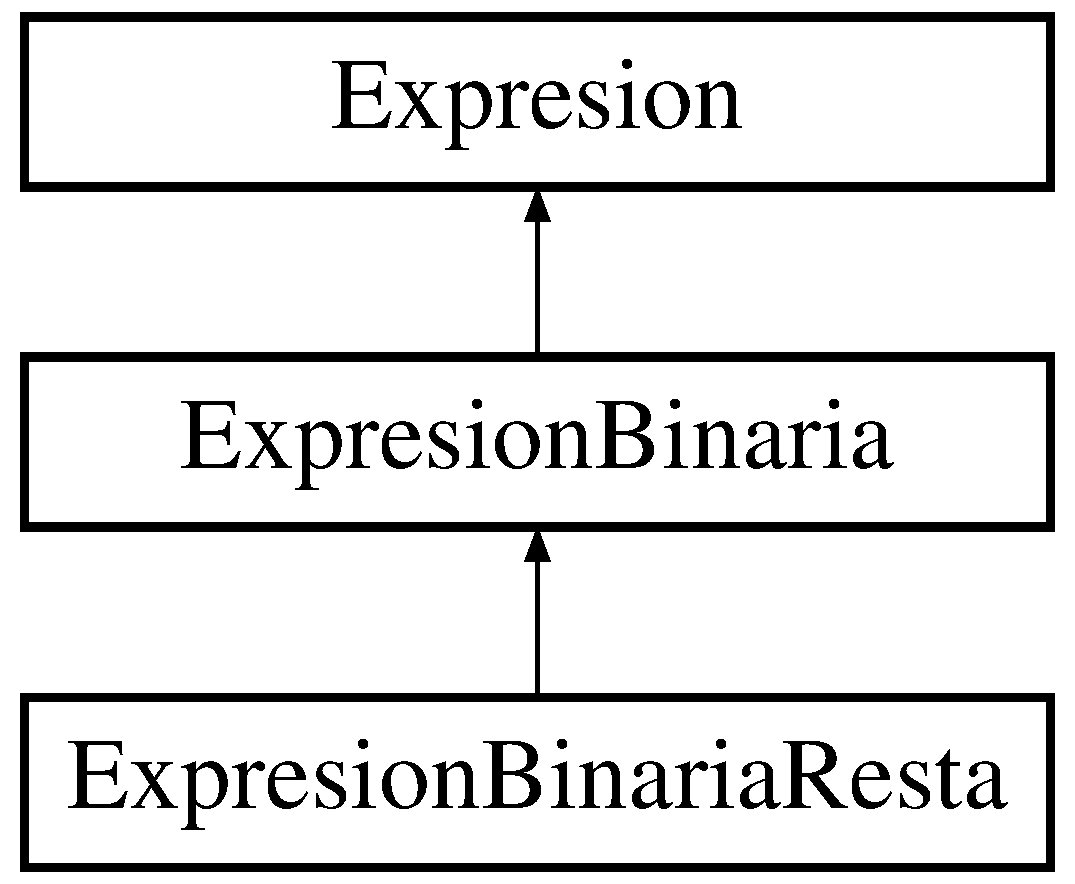
\includegraphics[height=3.000000cm]{class_expresion_binaria_resta}
\end{center}
\end{figure}
\subsection*{Métodos públicos}
\begin{DoxyCompactItemize}
\item 
\hypertarget{class_expresion_binaria_resta_a9b0be23838ca6ad1a4a5f7b937bebec3}{{\bfseries Expresion\-Binaria\-Resta} (\hyperlink{class_expresion}{Expresion} $\ast$izquierda, \hyperlink{class_expresion}{Expresion} $\ast$derecha, int numero\-De\-Linea)}\label{class_expresion_binaria_resta_a9b0be23838ca6ad1a4a5f7b937bebec3}

\item 
\hypertarget{class_expresion_binaria_resta_a726f776a505f953d71a9b0abebd09382}{virtual \hyperlink{class_tipo}{Tipo} $\ast$ {\bfseries validar\-Semantica} ()}\label{class_expresion_binaria_resta_a726f776a505f953d71a9b0abebd09382}

\item 
\hypertarget{class_expresion_binaria_resta_a0ff7e1880ebe673dd73230085633ae57}{virtual string {\bfseries generar\-Codigo\-Java} ()}\label{class_expresion_binaria_resta_a0ff7e1880ebe673dd73230085633ae57}

\end{DoxyCompactItemize}
\subsection*{Otros miembros heredados}


La documentación para esta clase fue generada a partir de los siguientes ficheros\-:\begin{DoxyCompactItemize}
\item 
Expresion/\-Expresion\-Binaria/Expresion\-Binaria\-Resta.\-h\item 
Expresion/\-Expresion\-Binaria/Expresion\-Binaria\-Resta.\-cpp\end{DoxyCompactItemize}

\hypertarget{class_expresion_binaria_suma}{\section{Referencia de la Clase Expresion\-Binaria\-Suma}
\label{class_expresion_binaria_suma}\index{Expresion\-Binaria\-Suma@{Expresion\-Binaria\-Suma}}
}
Diagrama de herencias de Expresion\-Binaria\-Suma\begin{figure}[H]
\begin{center}
\leavevmode
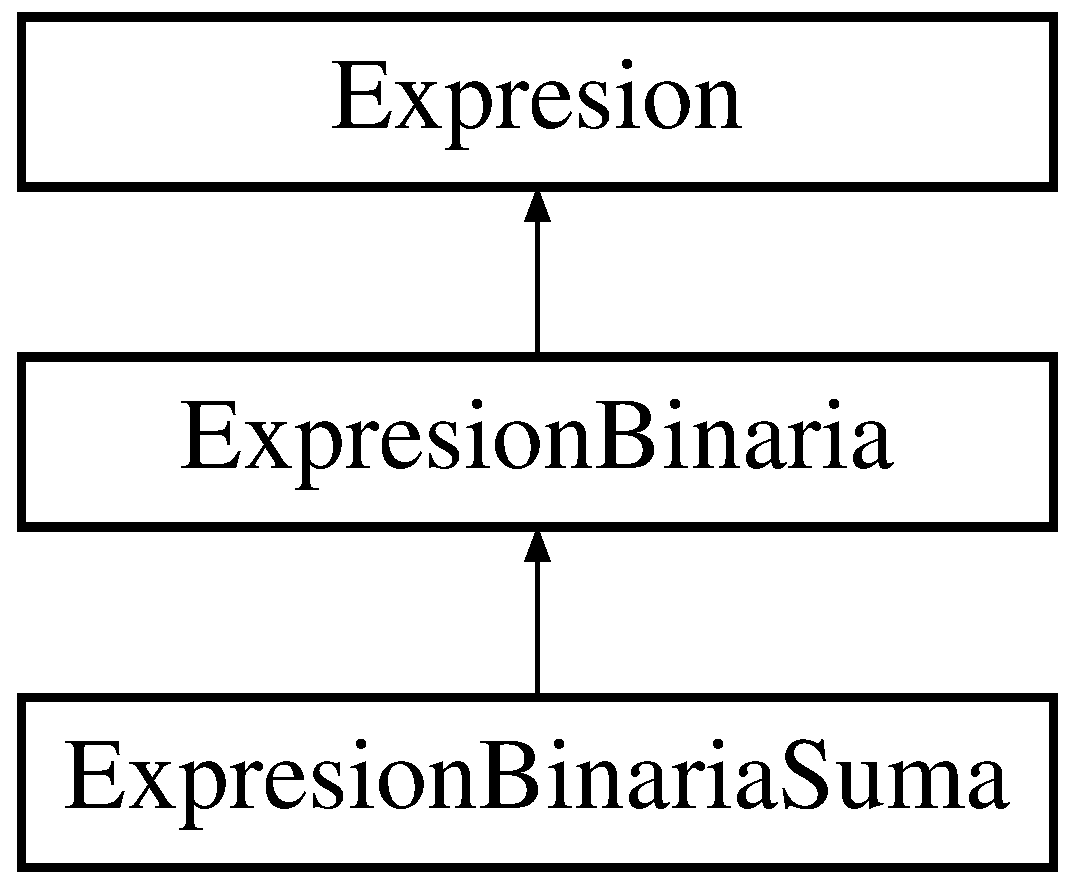
\includegraphics[height=3.000000cm]{class_expresion_binaria_suma}
\end{center}
\end{figure}
\subsection*{Métodos públicos}
\begin{DoxyCompactItemize}
\item 
\hypertarget{class_expresion_binaria_suma_a0b780585b562e896a101fd786371f5e0}{{\bfseries Expresion\-Binaria\-Suma} (\hyperlink{class_expresion}{Expresion} $\ast$izquierda, \hyperlink{class_expresion}{Expresion} $\ast$derecha, int numero\-De\-Linea)}\label{class_expresion_binaria_suma_a0b780585b562e896a101fd786371f5e0}

\item 
\hypertarget{class_expresion_binaria_suma_a19c9f4cc48473a7fa461ebc9a0b1938c}{virtual \hyperlink{class_tipo}{Tipo} $\ast$ {\bfseries validar\-Semantica} ()}\label{class_expresion_binaria_suma_a19c9f4cc48473a7fa461ebc9a0b1938c}

\item 
\hypertarget{class_expresion_binaria_suma_a82884b94e59727c09e7107ba5675d30b}{virtual string {\bfseries generar\-Codigo\-Java} ()}\label{class_expresion_binaria_suma_a82884b94e59727c09e7107ba5675d30b}

\end{DoxyCompactItemize}
\subsection*{Otros miembros heredados}


La documentación para esta clase fue generada a partir de los siguientes ficheros\-:\begin{DoxyCompactItemize}
\item 
Expresion/\-Expresion\-Binaria/Expresion\-Binaria\-Suma.\-h\item 
Expresion/\-Expresion\-Binaria/Expresion\-Binaria\-Suma.\-cpp\end{DoxyCompactItemize}

\hypertarget{class_expresion_binaria_y}{\section{Referencia de la Clase Expresion\-Binaria\-Y}
\label{class_expresion_binaria_y}\index{Expresion\-Binaria\-Y@{Expresion\-Binaria\-Y}}
}
Diagrama de herencias de Expresion\-Binaria\-Y\begin{figure}[H]
\begin{center}
\leavevmode
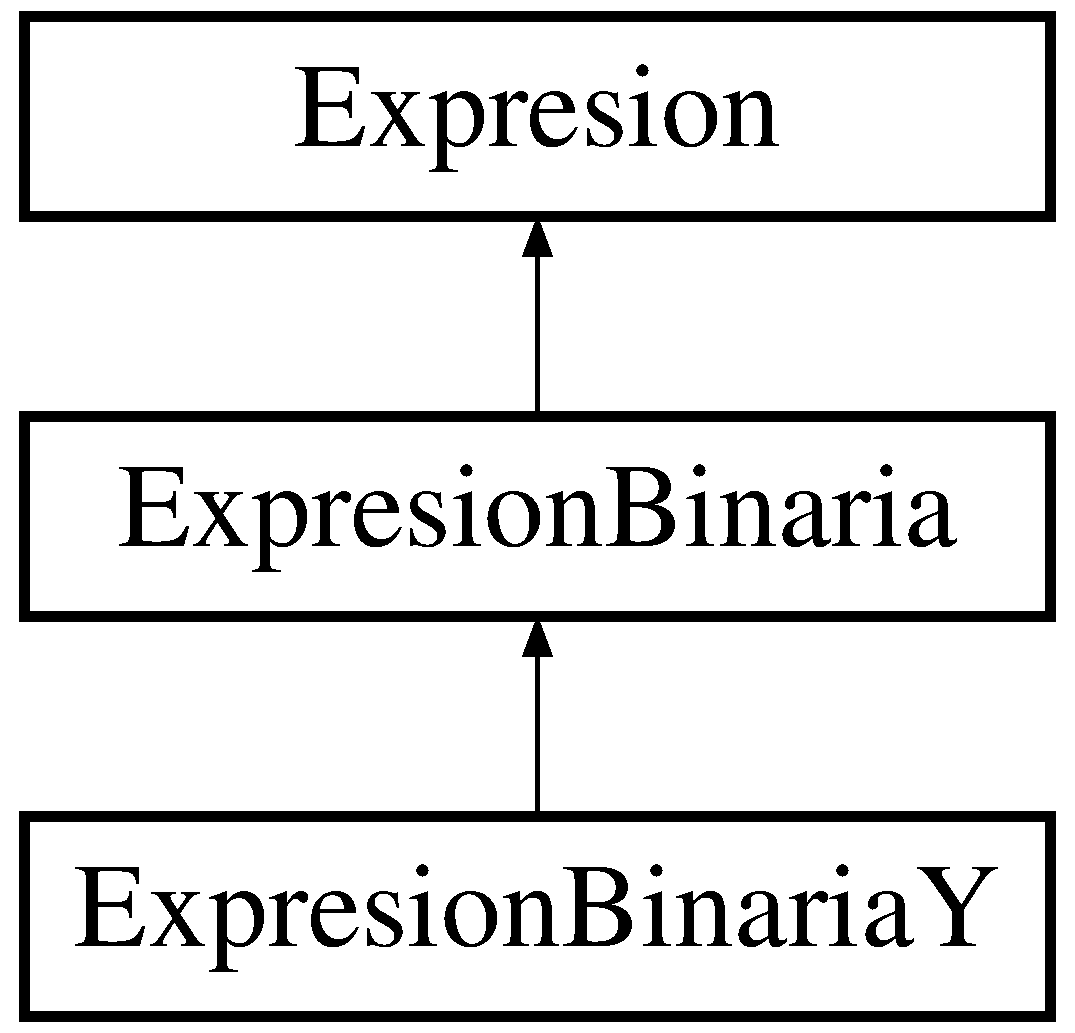
\includegraphics[height=3.000000cm]{class_expresion_binaria_y}
\end{center}
\end{figure}
\subsection*{Métodos públicos}
\begin{DoxyCompactItemize}
\item 
\hypertarget{class_expresion_binaria_y_a5f7fd923a07dca79556a75aec5ae1da7}{{\bfseries Expresion\-Binaria\-Y} (\hyperlink{class_expresion}{Expresion} $\ast$izquierda, \hyperlink{class_expresion}{Expresion} $\ast$derecha, int numero\-De\-Linea)}\label{class_expresion_binaria_y_a5f7fd923a07dca79556a75aec5ae1da7}

\item 
\hypertarget{class_expresion_binaria_y_aab6f1c529ea8c217962d57aad58184d4}{virtual \hyperlink{class_tipo}{Tipo} $\ast$ {\bfseries validar\-Semantica} ()}\label{class_expresion_binaria_y_aab6f1c529ea8c217962d57aad58184d4}

\item 
\hypertarget{class_expresion_binaria_y_a330a00b50de8bca9c62fc0af43b58d5e}{virtual string {\bfseries generar\-Codigo\-Java} ()}\label{class_expresion_binaria_y_a330a00b50de8bca9c62fc0af43b58d5e}

\end{DoxyCompactItemize}
\subsection*{Otros miembros heredados}


La documentación para esta clase fue generada a partir de los siguientes ficheros\-:\begin{DoxyCompactItemize}
\item 
Expresion/\-Expresion\-Binaria/Expresion\-Binaria\-Y.\-h\item 
Expresion/\-Expresion\-Binaria/Expresion\-Binaria\-Y.\-cpp\end{DoxyCompactItemize}

\hypertarget{class_expresion_instancia_de}{\section{Referencia de la Clase Expresion\-Instancia\-De}
\label{class_expresion_instancia_de}\index{Expresion\-Instancia\-De@{Expresion\-Instancia\-De}}
}
Diagrama de herencias de Expresion\-Instancia\-De\begin{figure}[H]
\begin{center}
\leavevmode
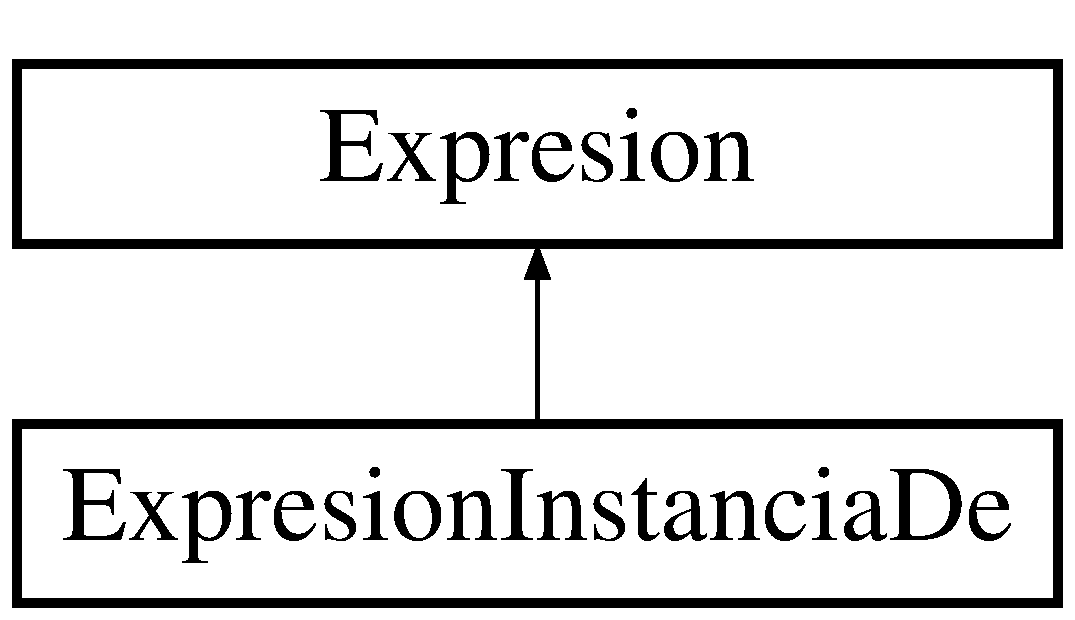
\includegraphics[height=2.000000cm]{class_expresion_instancia_de}
\end{center}
\end{figure}
\subsection*{Métodos públicos}
\begin{DoxyCompactItemize}
\item 
\hypertarget{class_expresion_instancia_de_a901569629da3b94f17587a5e97a8d201}{{\bfseries Expresion\-Instancia\-De} (\hyperlink{class_expresion}{Expresion} $\ast$expresion, Tipo\-Dato tipo\-Dato, int numero\-De\-Linea)}\label{class_expresion_instancia_de_a901569629da3b94f17587a5e97a8d201}

\item 
\hypertarget{class_expresion_instancia_de_aa6383a6e850df716d09a5b306082014e}{virtual \hyperlink{class_tipo}{Tipo} $\ast$ {\bfseries validar\-Semantica} ()}\label{class_expresion_instancia_de_aa6383a6e850df716d09a5b306082014e}

\item 
\hypertarget{class_expresion_instancia_de_a74422da6614660d75a77a3a6011b9fcf}{virtual string {\bfseries generar\-Codigo\-Java} ()}\label{class_expresion_instancia_de_a74422da6614660d75a77a3a6011b9fcf}

\end{DoxyCompactItemize}
\subsection*{Otros miembros heredados}


La documentación para esta clase fue generada a partir de los siguientes ficheros\-:\begin{DoxyCompactItemize}
\item 
Expresion/Expresion\-Instancia\-De.\-h\item 
Expresion/Expresion\-Instancia\-De.\-cpp\end{DoxyCompactItemize}

\hypertarget{class_expresion_literal_booleana}{\section{Referencia de la Clase Expresion\-Literal\-Booleana}
\label{class_expresion_literal_booleana}\index{Expresion\-Literal\-Booleana@{Expresion\-Literal\-Booleana}}
}
Diagrama de herencias de Expresion\-Literal\-Booleana\begin{figure}[H]
\begin{center}
\leavevmode
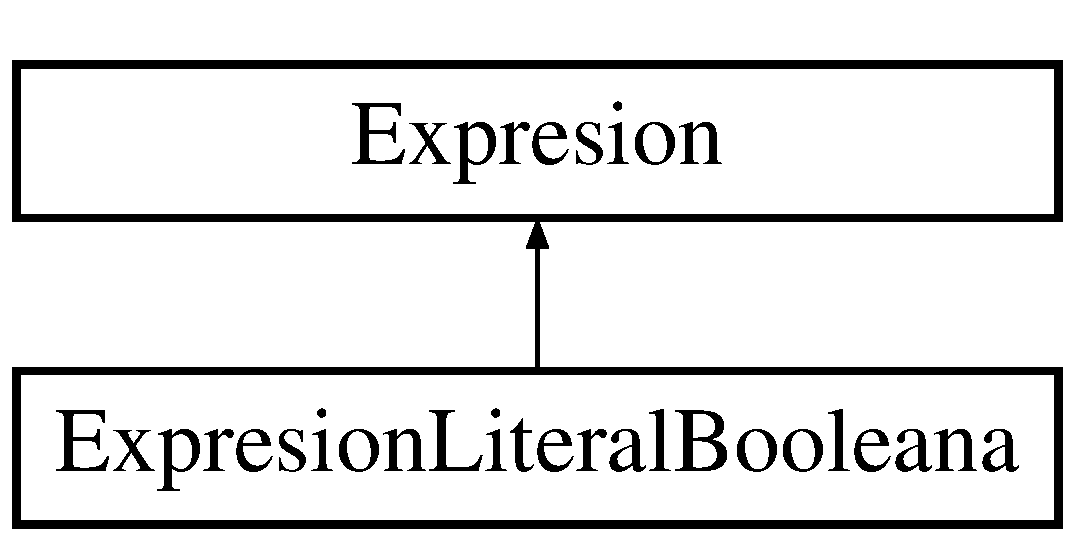
\includegraphics[height=2.000000cm]{class_expresion_literal_booleana}
\end{center}
\end{figure}
\subsection*{Métodos públicos}
\begin{DoxyCompactItemize}
\item 
\hypertarget{class_expresion_literal_booleana_a897dfa8b6bf7bb31875047843eb2d9ff}{{\bfseries Expresion\-Literal\-Booleana} (bool valor, int numero\-De\-Linea)}\label{class_expresion_literal_booleana_a897dfa8b6bf7bb31875047843eb2d9ff}

\item 
\hypertarget{class_expresion_literal_booleana_a83b1438c05f149292bad559b31843755}{virtual \hyperlink{class_tipo}{Tipo} $\ast$ {\bfseries validar\-Semantica} ()}\label{class_expresion_literal_booleana_a83b1438c05f149292bad559b31843755}

\item 
\hypertarget{class_expresion_literal_booleana_a3c4e9a857e89bd40ee1b94c0620ae668}{virtual string {\bfseries generar\-Codigo\-Java} ()}\label{class_expresion_literal_booleana_a3c4e9a857e89bd40ee1b94c0620ae668}

\end{DoxyCompactItemize}
\subsection*{Otros miembros heredados}


La documentación para esta clase fue generada a partir de los siguientes ficheros\-:\begin{DoxyCompactItemize}
\item 
Expresion/\-Expresion\-Literal/Expresion\-Literal\-Booleana.\-h\item 
Expresion/\-Expresion\-Literal/Expresion\-Literal\-Booleana.\-cpp\end{DoxyCompactItemize}

\hypertarget{class_expresion_literal_cadena}{\section{Referencia de la Clase Expresion\-Literal\-Cadena}
\label{class_expresion_literal_cadena}\index{Expresion\-Literal\-Cadena@{Expresion\-Literal\-Cadena}}
}
Diagrama de herencias de Expresion\-Literal\-Cadena\begin{figure}[H]
\begin{center}
\leavevmode
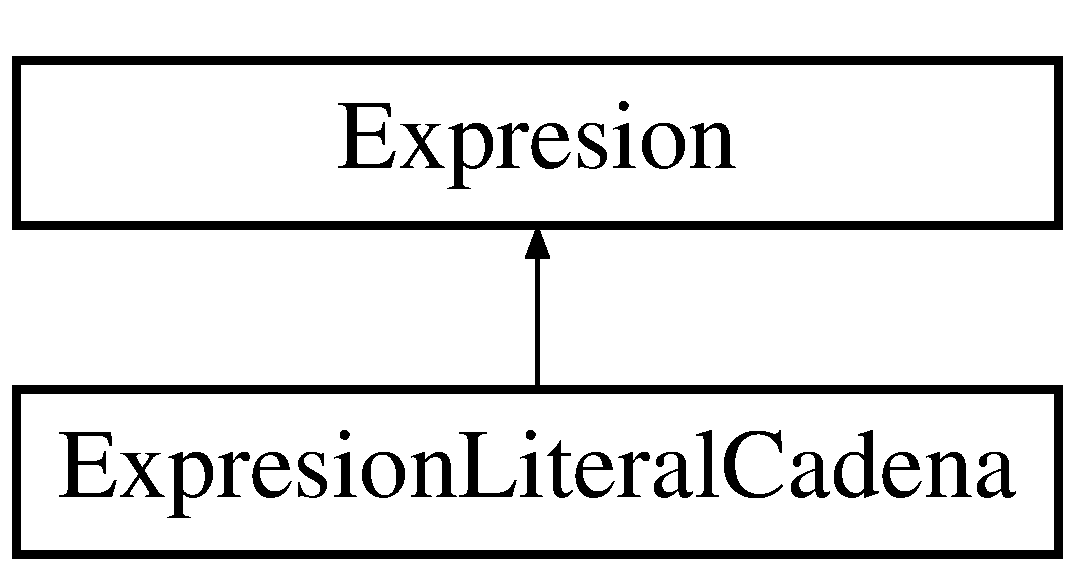
\includegraphics[height=2.000000cm]{class_expresion_literal_cadena}
\end{center}
\end{figure}
\subsection*{Métodos públicos}
\begin{DoxyCompactItemize}
\item 
\hypertarget{class_expresion_literal_cadena_a94d7c37cbc811885a48522b4832f1731}{{\bfseries Expresion\-Literal\-Cadena} (string $\ast$valor, int numero\-De\-Linea)}\label{class_expresion_literal_cadena_a94d7c37cbc811885a48522b4832f1731}

\item 
\hypertarget{class_expresion_literal_cadena_a0e49a3a889692e29f17e9a0064492558}{virtual \hyperlink{class_tipo}{Tipo} $\ast$ {\bfseries validar\-Semantica} ()}\label{class_expresion_literal_cadena_a0e49a3a889692e29f17e9a0064492558}

\item 
\hypertarget{class_expresion_literal_cadena_a6e2ea52a5a236281e8382d82a3a8bba7}{virtual string {\bfseries generar\-Codigo\-Java} ()}\label{class_expresion_literal_cadena_a6e2ea52a5a236281e8382d82a3a8bba7}

\end{DoxyCompactItemize}
\subsection*{Otros miembros heredados}


La documentación para esta clase fue generada a partir de los siguientes ficheros\-:\begin{DoxyCompactItemize}
\item 
Expresion/\-Expresion\-Literal/Expresion\-Literal\-Cadena.\-h\item 
Expresion/\-Expresion\-Literal/Expresion\-Literal\-Cadena.\-cpp\end{DoxyCompactItemize}

\hypertarget{class_expresion_literal_caracter}{\section{Referencia de la Clase Expresion\-Literal\-Caracter}
\label{class_expresion_literal_caracter}\index{Expresion\-Literal\-Caracter@{Expresion\-Literal\-Caracter}}
}
Diagrama de herencias de Expresion\-Literal\-Caracter\begin{figure}[H]
\begin{center}
\leavevmode
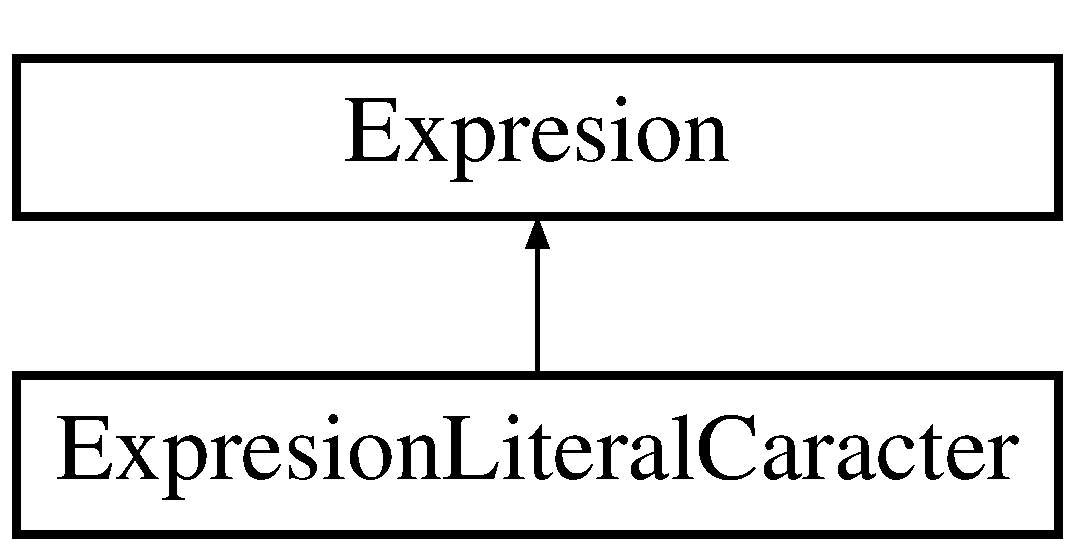
\includegraphics[height=2.000000cm]{class_expresion_literal_caracter}
\end{center}
\end{figure}
\subsection*{Métodos públicos}
\begin{DoxyCompactItemize}
\item 
\hypertarget{class_expresion_literal_caracter_ab2927730e3b84b9d435c0c4c52fd6726}{{\bfseries Expresion\-Literal\-Caracter} (char valor, int numero\-De\-Linea)}\label{class_expresion_literal_caracter_ab2927730e3b84b9d435c0c4c52fd6726}

\item 
\hypertarget{class_expresion_literal_caracter_a178394c347ea98a4eeb489adabe5f5b0}{virtual \hyperlink{class_tipo}{Tipo} $\ast$ {\bfseries validar\-Semantica} ()}\label{class_expresion_literal_caracter_a178394c347ea98a4eeb489adabe5f5b0}

\item 
\hypertarget{class_expresion_literal_caracter_aa4894fa895257bce99a6bf9dbe1d4d03}{virtual string {\bfseries generar\-Codigo\-Java} ()}\label{class_expresion_literal_caracter_aa4894fa895257bce99a6bf9dbe1d4d03}

\end{DoxyCompactItemize}
\subsection*{Otros miembros heredados}


La documentación para esta clase fue generada a partir de los siguientes ficheros\-:\begin{DoxyCompactItemize}
\item 
Expresion/\-Expresion\-Literal/Expresion\-Literal\-Caracter.\-h\item 
Expresion/\-Expresion\-Literal/Expresion\-Literal\-Caracter.\-cpp\end{DoxyCompactItemize}

\hypertarget{class_expresion_literal_entera}{\section{Referencia de la Clase Expresion\-Literal\-Entera}
\label{class_expresion_literal_entera}\index{Expresion\-Literal\-Entera@{Expresion\-Literal\-Entera}}
}
Diagrama de herencias de Expresion\-Literal\-Entera\begin{figure}[H]
\begin{center}
\leavevmode
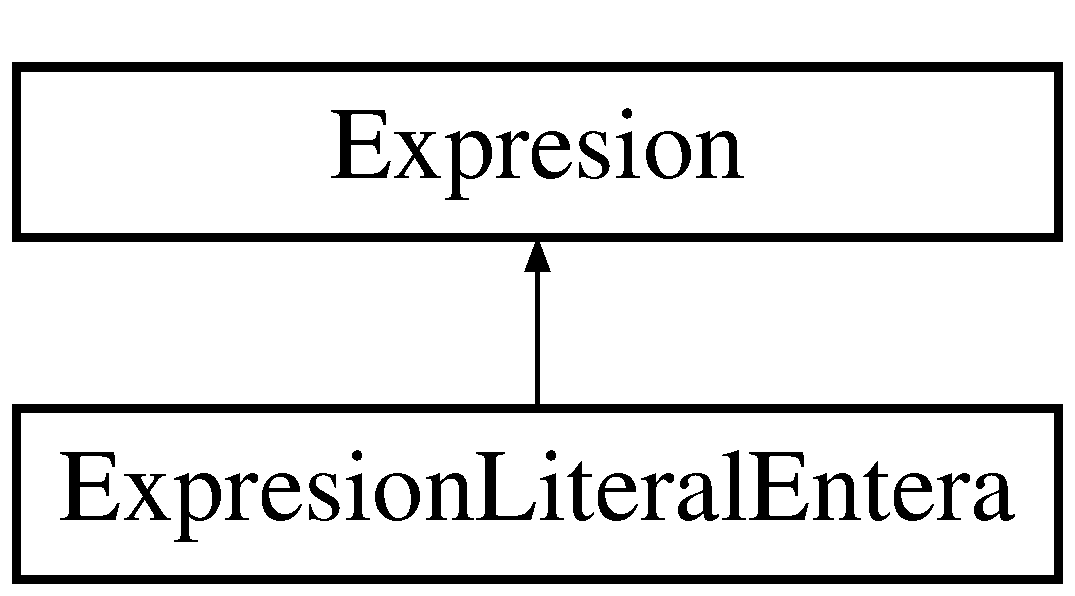
\includegraphics[height=2.000000cm]{class_expresion_literal_entera}
\end{center}
\end{figure}
\subsection*{Métodos públicos}
\begin{DoxyCompactItemize}
\item 
\hypertarget{class_expresion_literal_entera_af9fbcbcf1980e9b88d336ec8341a5b5f}{{\bfseries Expresion\-Literal\-Entera} (int valor, int numero\-De\-Linea)}\label{class_expresion_literal_entera_af9fbcbcf1980e9b88d336ec8341a5b5f}

\item 
\hypertarget{class_expresion_literal_entera_ae70eb9a5ae257722518571e8b588b784}{virtual \hyperlink{class_tipo}{Tipo} $\ast$ {\bfseries validar\-Semantica} ()}\label{class_expresion_literal_entera_ae70eb9a5ae257722518571e8b588b784}

\item 
\hypertarget{class_expresion_literal_entera_a3805de0b11acedef3cdac86730f4eadc}{virtual string {\bfseries generar\-Codigo\-Java} ()}\label{class_expresion_literal_entera_a3805de0b11acedef3cdac86730f4eadc}

\end{DoxyCompactItemize}
\subsection*{Otros miembros heredados}


La documentación para esta clase fue generada a partir de los siguientes ficheros\-:\begin{DoxyCompactItemize}
\item 
Expresion/\-Expresion\-Literal/Expresion\-Literal\-Entera.\-h\item 
Expresion/\-Expresion\-Literal/Expresion\-Literal\-Entera.\-cpp\end{DoxyCompactItemize}

\hypertarget{class_expresion_literal_flotante}{\section{Referencia de la Clase Expresion\-Literal\-Flotante}
\label{class_expresion_literal_flotante}\index{Expresion\-Literal\-Flotante@{Expresion\-Literal\-Flotante}}
}
Diagrama de herencias de Expresion\-Literal\-Flotante\begin{figure}[H]
\begin{center}
\leavevmode
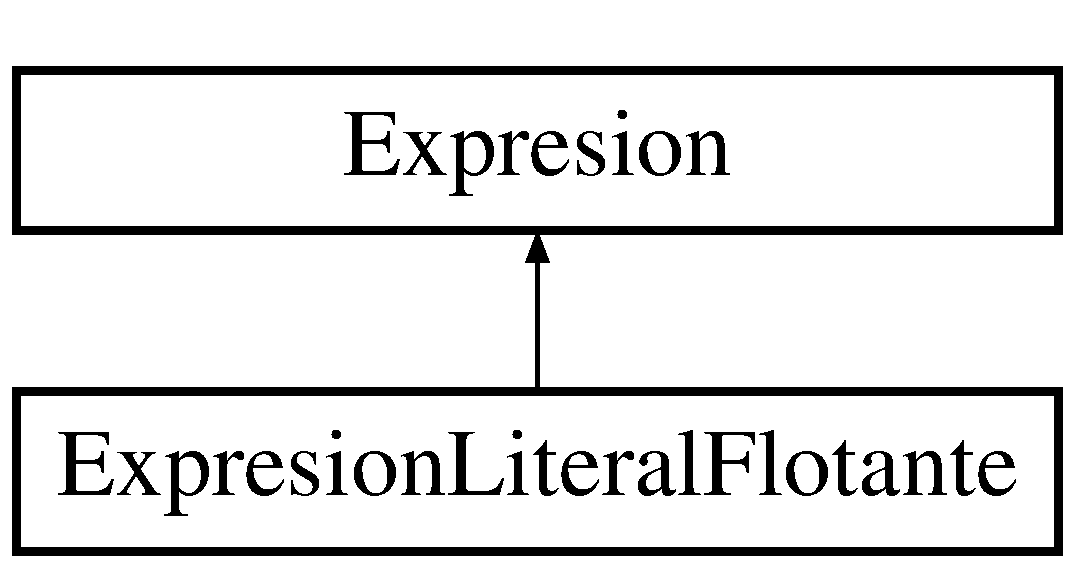
\includegraphics[height=2.000000cm]{class_expresion_literal_flotante}
\end{center}
\end{figure}
\subsection*{Métodos públicos}
\begin{DoxyCompactItemize}
\item 
\hypertarget{class_expresion_literal_flotante_aa665968af6490edaa0d39b5c492d1a66}{{\bfseries Expresion\-Literal\-Flotante} (float valor, int numero\-De\-Linea)}\label{class_expresion_literal_flotante_aa665968af6490edaa0d39b5c492d1a66}

\item 
\hypertarget{class_expresion_literal_flotante_af76f6c6bdcbeb52bf21181816cb467cd}{virtual \hyperlink{class_tipo}{Tipo} $\ast$ {\bfseries validar\-Semantica} ()}\label{class_expresion_literal_flotante_af76f6c6bdcbeb52bf21181816cb467cd}

\item 
\hypertarget{class_expresion_literal_flotante_a2bbdfdf8c949d75b5b3987ba8698cc25}{virtual string {\bfseries generar\-Codigo\-Java} ()}\label{class_expresion_literal_flotante_a2bbdfdf8c949d75b5b3987ba8698cc25}

\end{DoxyCompactItemize}
\subsection*{Otros miembros heredados}


La documentación para esta clase fue generada a partir de los siguientes ficheros\-:\begin{DoxyCompactItemize}
\item 
Expresion/\-Expresion\-Literal/Expresion\-Literal\-Flotante.\-h\item 
Expresion/\-Expresion\-Literal/Expresion\-Literal\-Flotante.\-cpp\end{DoxyCompactItemize}

\hypertarget{class_expresion_unaria}{\section{Referencia de la Clase Expresion\-Unaria}
\label{class_expresion_unaria}\index{Expresion\-Unaria@{Expresion\-Unaria}}
}
Diagrama de herencias de Expresion\-Unaria\begin{figure}[H]
\begin{center}
\leavevmode
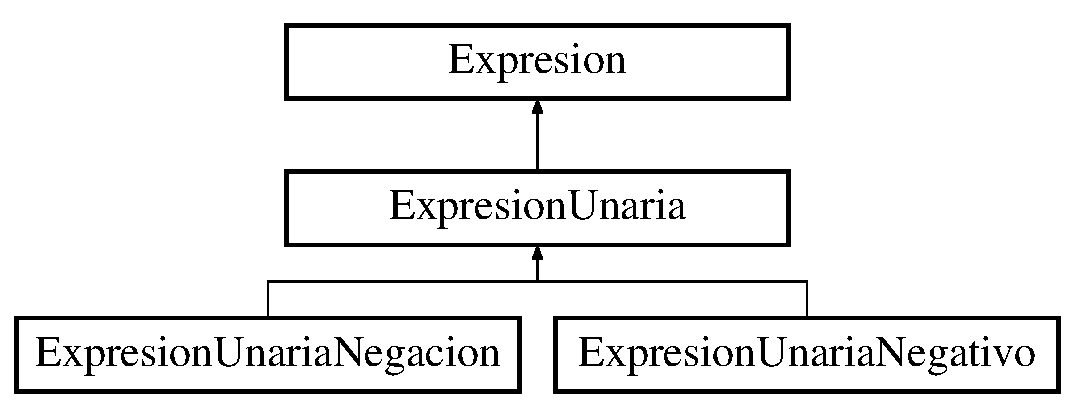
\includegraphics[height=3.000000cm]{class_expresion_unaria}
\end{center}
\end{figure}
\subsection*{Métodos públicos}
\begin{DoxyCompactItemize}
\item 
\hypertarget{class_expresion_unaria_a85140ab958ab019f4ee572b48eaacb05}{{\bfseries Expresion\-Unaria} (\hyperlink{class_expresion}{Expresion} $\ast$expresion, Expresiones tipo, int numero\-De\-Linea)}\label{class_expresion_unaria_a85140ab958ab019f4ee572b48eaacb05}

\item 
\hypertarget{class_expresion_unaria_a9d2b8382b86dadef390bc9cbbd480ad1}{\hyperlink{class_expresion}{Expresion} $\ast$ {\bfseries obtener\-Expresion} ()}\label{class_expresion_unaria_a9d2b8382b86dadef390bc9cbbd480ad1}

\end{DoxyCompactItemize}
\subsection*{Otros miembros heredados}


La documentación para esta clase fue generada a partir de los siguientes ficheros\-:\begin{DoxyCompactItemize}
\item 
Expresion/\-Expresion\-Unaria/Expresion\-Unaria.\-h\item 
Expresion/\-Expresion\-Unaria/Expresion\-Unaria.\-cpp\end{DoxyCompactItemize}

\hypertarget{class_expresion_unaria_negacion}{\section{Referencia de la Clase Expresion\-Unaria\-Negacion}
\label{class_expresion_unaria_negacion}\index{Expresion\-Unaria\-Negacion@{Expresion\-Unaria\-Negacion}}
}
Diagrama de herencias de Expresion\-Unaria\-Negacion\begin{figure}[H]
\begin{center}
\leavevmode
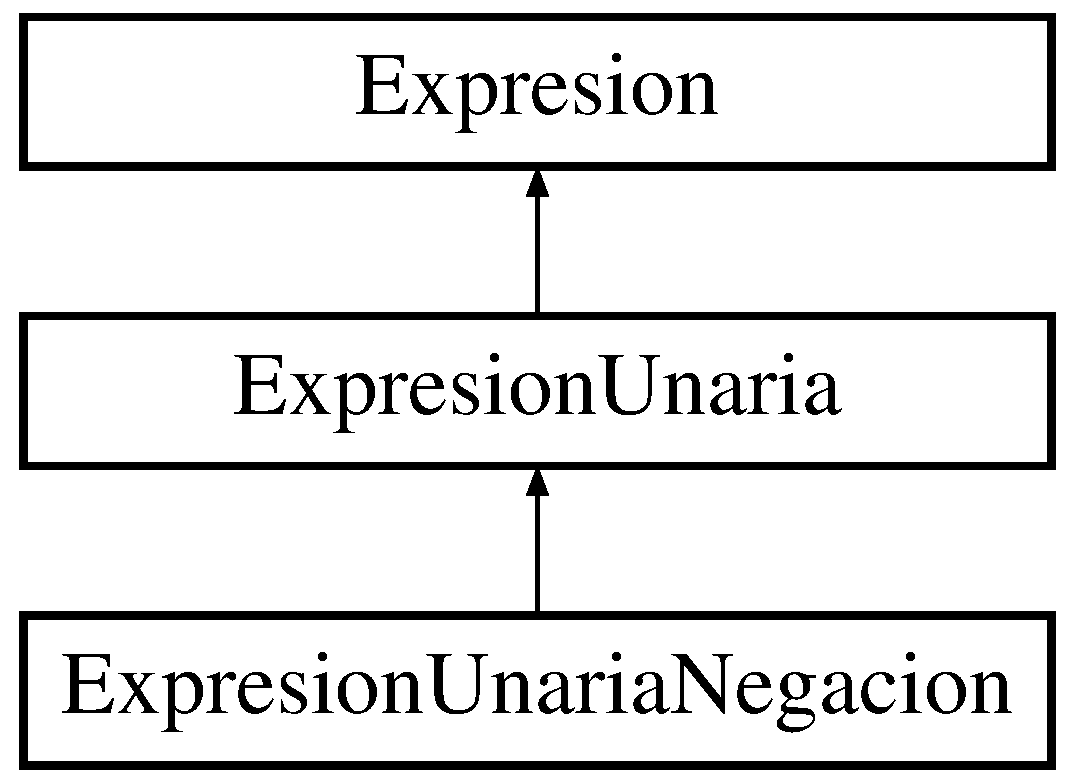
\includegraphics[height=3.000000cm]{class_expresion_unaria_negacion}
\end{center}
\end{figure}
\subsection*{Métodos públicos}
\begin{DoxyCompactItemize}
\item 
\hypertarget{class_expresion_unaria_negacion_aada4302b36facccbae7293378bf8c57d}{{\bfseries Expresion\-Unaria\-Negacion} (\hyperlink{class_expresion}{Expresion} $\ast$expresion, int numero\-De\-Linea)}\label{class_expresion_unaria_negacion_aada4302b36facccbae7293378bf8c57d}

\item 
\hypertarget{class_expresion_unaria_negacion_a23d0730b5c388fac4fc7f61744d0933d}{virtual \hyperlink{class_tipo}{Tipo} $\ast$ {\bfseries validar\-Semantica} ()}\label{class_expresion_unaria_negacion_a23d0730b5c388fac4fc7f61744d0933d}

\item 
\hypertarget{class_expresion_unaria_negacion_a27678c55ab7dbdfc59c9c83b60c970c4}{virtual string {\bfseries generar\-Codigo\-Java} ()}\label{class_expresion_unaria_negacion_a27678c55ab7dbdfc59c9c83b60c970c4}

\end{DoxyCompactItemize}
\subsection*{Otros miembros heredados}


La documentación para esta clase fue generada a partir de los siguientes ficheros\-:\begin{DoxyCompactItemize}
\item 
Expresion/\-Expresion\-Unaria/Expresion\-Unaria\-Negacion.\-h\item 
Expresion/\-Expresion\-Unaria/Expresion\-Unaria\-Negacion.\-cpp\end{DoxyCompactItemize}

\hypertarget{class_expresion_unaria_negativo}{\section{Referencia de la Clase Expresion\-Unaria\-Negativo}
\label{class_expresion_unaria_negativo}\index{Expresion\-Unaria\-Negativo@{Expresion\-Unaria\-Negativo}}
}
Diagrama de herencias de Expresion\-Unaria\-Negativo\begin{figure}[H]
\begin{center}
\leavevmode
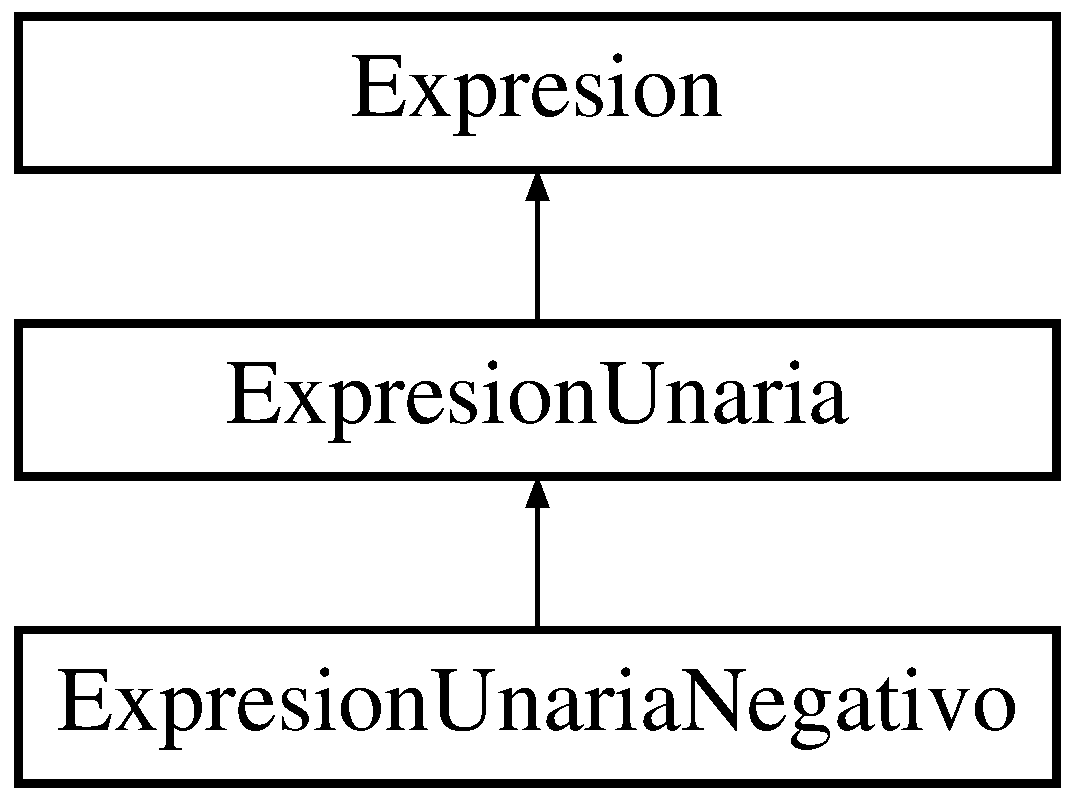
\includegraphics[height=3.000000cm]{class_expresion_unaria_negativo}
\end{center}
\end{figure}
\subsection*{Métodos públicos}
\begin{DoxyCompactItemize}
\item 
\hypertarget{class_expresion_unaria_negativo_a897ba7b63c8c8d6d7c5794a27dcb322b}{{\bfseries Expresion\-Unaria\-Negativo} (\hyperlink{class_expresion}{Expresion} $\ast$expresion, int numero\-De\-Linea)}\label{class_expresion_unaria_negativo_a897ba7b63c8c8d6d7c5794a27dcb322b}

\item 
\hypertarget{class_expresion_unaria_negativo_a876ebfb1a2ac9546a696078b6a18381c}{virtual \hyperlink{class_tipo}{Tipo} $\ast$ {\bfseries validar\-Semantica} ()}\label{class_expresion_unaria_negativo_a876ebfb1a2ac9546a696078b6a18381c}

\item 
\hypertarget{class_expresion_unaria_negativo_a0bfb774ec66fda7bfcb88f403026265e}{virtual string {\bfseries generar\-Codigo\-Java} ()}\label{class_expresion_unaria_negativo_a0bfb774ec66fda7bfcb88f403026265e}

\end{DoxyCompactItemize}
\subsection*{Otros miembros heredados}


La documentación para esta clase fue generada a partir de los siguientes ficheros\-:\begin{DoxyCompactItemize}
\item 
Expresion/\-Expresion\-Unaria/Expresion\-Unaria\-Negativo.\-h\item 
Expresion/\-Expresion\-Unaria/Expresion\-Unaria\-Negativo.\-cpp\end{DoxyCompactItemize}

\hypertarget{class_funcion}{\section{Referencia de la Clase Funcion}
\label{class_funcion}\index{Funcion@{Funcion}}
}
\subsection*{Métodos públicos}
\begin{DoxyCompactItemize}
\item 
\hypertarget{class_funcion_a01b8d581259b1f982c25c3e734a2188d}{{\bfseries Funcion} (\hyperlink{class_tipo}{Tipo} $\ast$tipo\-De\-Retorno, vector$<$ Tipo\-Parametro $>$ $\ast$parametros)}\label{class_funcion_a01b8d581259b1f982c25c3e734a2188d}

\item 
\hypertarget{class_funcion_a1912c4a74bfed025ebb6e78c26532709}{{\bfseries Funcion} (\hyperlink{class_tipo}{Tipo} $\ast$tipo\-De\-Retorno, vector$<$ Tipo\-Parametro $>$ $\ast$parametros, string $\ast$codigo)}\label{class_funcion_a1912c4a74bfed025ebb6e78c26532709}

\end{DoxyCompactItemize}
\subsection*{Atributos públicos}
\begin{DoxyCompactItemize}
\item 
\hypertarget{class_funcion_aaaa7553fc7b60f80a86e321e36854968}{\hyperlink{class_tipo}{Tipo} $\ast$ {\bfseries tipo\-De\-Retorno}}\label{class_funcion_aaaa7553fc7b60f80a86e321e36854968}

\item 
\hypertarget{class_funcion_aa7139ebb9c92733298382ab128ae9b00}{vector$<$ Tipo\-Parametro $>$ $\ast$ {\bfseries parametros}}\label{class_funcion_aa7139ebb9c92733298382ab128ae9b00}

\item 
\hypertarget{class_funcion_aabc2121cdc6c8907b279c85671689b22}{string $\ast$ {\bfseries codigo}}\label{class_funcion_aabc2121cdc6c8907b279c85671689b22}

\end{DoxyCompactItemize}


La documentación para esta clase fue generada a partir de los siguientes ficheros\-:\begin{DoxyCompactItemize}
\item 
Programa/Funcion.\-h\item 
Programa/Funcion.\-cpp\end{DoxyCompactItemize}

\hypertarget{class_funciones_incorporadas}{\section{Referencia de la Clase Funciones\-Incorporadas}
\label{class_funciones_incorporadas}\index{Funciones\-Incorporadas@{Funciones\-Incorporadas}}
}
\subsection*{Métodos públicos}
\begin{DoxyCompactItemize}
\item 
\hypertarget{class_funciones_incorporadas_a7377645093c2d5bb19674897ced60570}{map$<$ string, \hyperlink{class_funcion}{Funcion} $\ast$ $>$ $\ast$ {\bfseries obtener\-Funciones\-Incorporadas} ()}\label{class_funciones_incorporadas_a7377645093c2d5bb19674897ced60570}

\item 
\hypertarget{class_funciones_incorporadas_a724b8dc70b2d0d4eb051578cadc3f0ca}{map$<$ string, string $>$ $\ast$ {\bfseries obtener\-Codigo\-Funciones} ()}\label{class_funciones_incorporadas_a724b8dc70b2d0d4eb051578cadc3f0ca}

\end{DoxyCompactItemize}


La documentación para esta clase fue generada a partir de los siguientes ficheros\-:\begin{DoxyCompactItemize}
\item 
Programa/Funciones\-Incorporadas.\-h\item 
Programa/Funciones\-Incorporadas (\-Copia conflictiva de siwady-\/\-P\-C 2013-\/02-\/16).\-cpp\item 
Programa/Funciones\-Incorporadas.\-cpp\end{DoxyCompactItemize}

\hypertarget{class_funcion_utilizada}{\section{Referencia de la Clase Funcion\-Utilizada}
\label{class_funcion_utilizada}\index{Funcion\-Utilizada@{Funcion\-Utilizada}}
}


La documentación para esta clase fue generada a partir de los siguientes ficheros\-:\begin{DoxyCompactItemize}
\item 
Programa/Funcion\-Utilizada.\-h\item 
Programa/Funcion\-Utilizada.\-cpp\end{DoxyCompactItemize}

\hypertarget{class_generador_de_errores}{\section{Referencia de la Clase Generador\-De\-Errores}
\label{class_generador_de_errores}\index{Generador\-De\-Errores@{Generador\-De\-Errores}}
}
\subsection*{Métodos públicos estáticos}
\begin{DoxyCompactItemize}
\item 
\hypertarget{class_generador_de_errores_a761a25b0838acc443d3d91fbecc46298}{static string {\bfseries obtener\-Token\-Esperado} (int numero\-De\-Token)}\label{class_generador_de_errores_a761a25b0838acc443d3d91fbecc46298}

\end{DoxyCompactItemize}


La documentación para esta clase fue generada a partir de los siguientes ficheros\-:\begin{DoxyCompactItemize}
\item 
Programa/Generador\-De\-Errores.\-h\item 
Programa/Generador\-De\-Errores.\-cpp\end{DoxyCompactItemize}

\hypertarget{class_instruccion}{\section{Referencia de la Clase Instruccion}
\label{class_instruccion}\index{Instruccion@{Instruccion}}
}
Diagrama de herencias de Instruccion\begin{figure}[H]
\begin{center}
\leavevmode
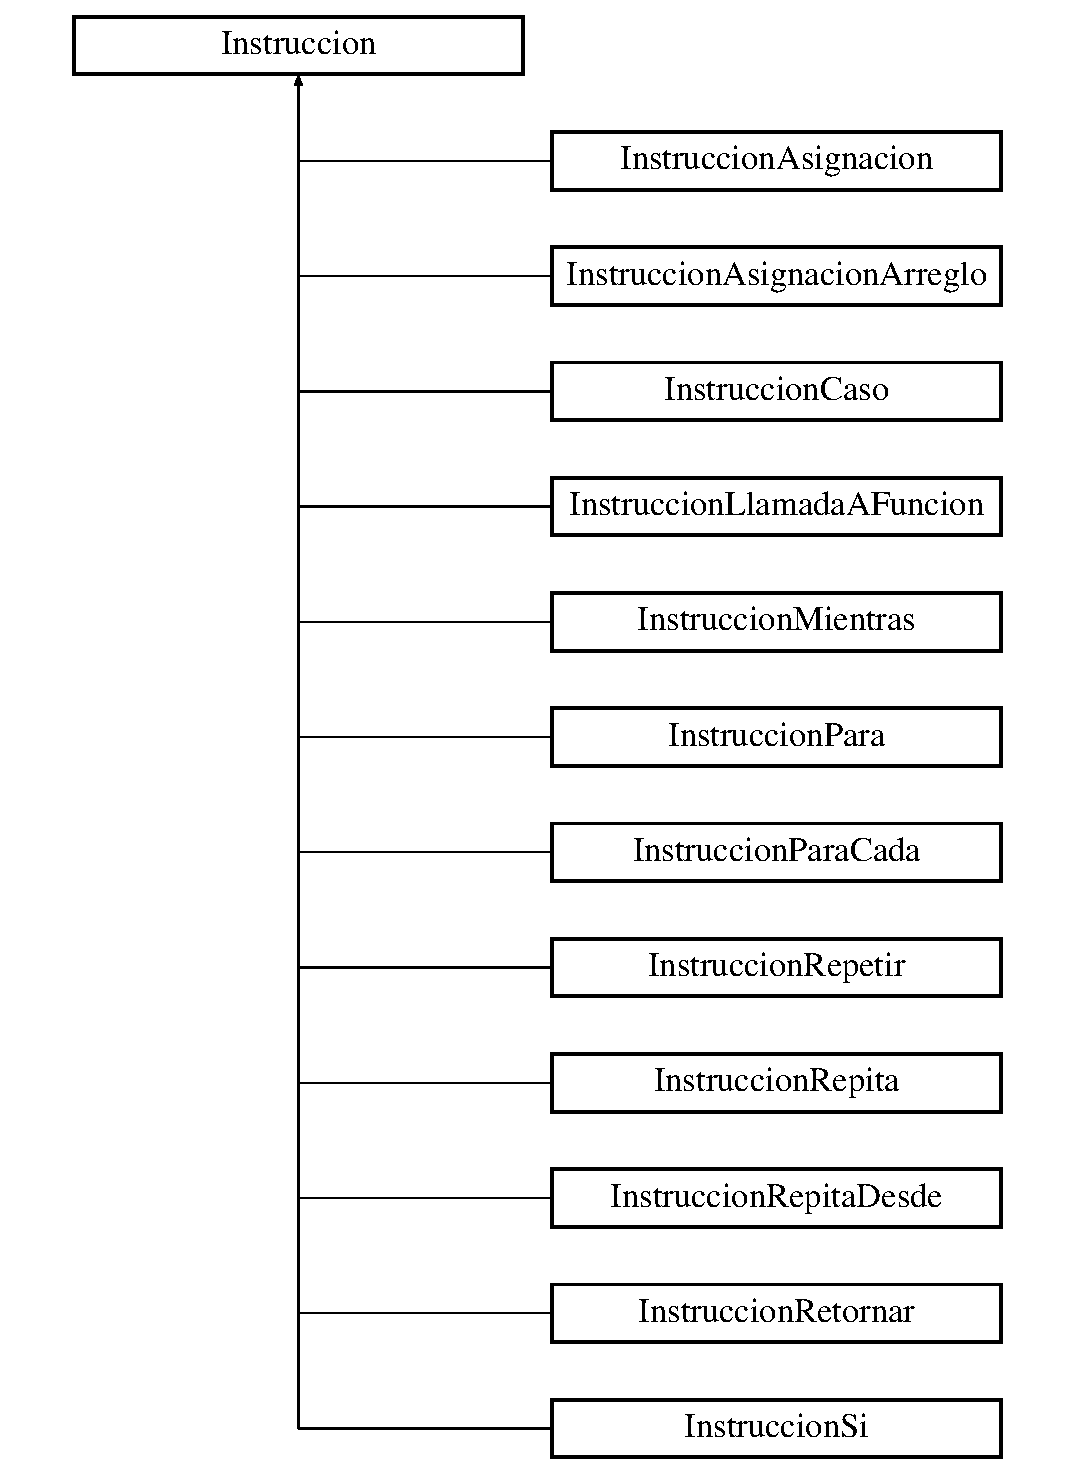
\includegraphics[height=12.000000cm]{class_instruccion}
\end{center}
\end{figure}
\subsection*{Métodos públicos}
\begin{DoxyCompactItemize}
\item 
\hypertarget{class_instruccion_ac488690feaf3f74fb5f140135aa57443}{{\bfseries Instruccion} (\hyperlink{class_instruccion}{Instruccion} $\ast$siguiente, Instrucciones tipo, int id\-De\-Expresion, int numero\-De\-Linea)}\label{class_instruccion_ac488690feaf3f74fb5f140135aa57443}

\item 
\hypertarget{class_instruccion_aa7def8e8c05017486c73e3f66462f0b0}{void {\bfseries establecer\-Siguiente} (\hyperlink{class_instruccion}{Instruccion} $\ast$siguiente)}\label{class_instruccion_aa7def8e8c05017486c73e3f66462f0b0}

\item 
\hypertarget{class_instruccion_ae353ca3aa158c3cf6ae5597e078301c4}{\hyperlink{class_instruccion}{Instruccion} $\ast$ {\bfseries obtener\-Siguiente} ()}\label{class_instruccion_ae353ca3aa158c3cf6ae5597e078301c4}

\item 
\hypertarget{class_instruccion_a3221facd5e7fa4a41c2314e9f178a565}{Instrucciones {\bfseries obtener\-Tipo} ()}\label{class_instruccion_a3221facd5e7fa4a41c2314e9f178a565}

\item 
\hypertarget{class_instruccion_abf4bdd28d62ec646e5cf8fb735b997ab}{virtual void {\bfseries validar\-Semantica} ()=0}\label{class_instruccion_abf4bdd28d62ec646e5cf8fb735b997ab}

\item 
\hypertarget{class_instruccion_acb14226a5a304cd5c9abe69ac6143edb}{virtual string {\bfseries generar\-Codigo\-Java} ()=0}\label{class_instruccion_acb14226a5a304cd5c9abe69ac6143edb}

\end{DoxyCompactItemize}
\subsection*{Atributos públicos}
\begin{DoxyCompactItemize}
\item 
\hypertarget{class_instruccion_a55f89a7724ad2e918bc8bd03be885d1c}{int {\bfseries numero\-De\-Linea}}\label{class_instruccion_a55f89a7724ad2e918bc8bd03be885d1c}

\end{DoxyCompactItemize}


La documentación para esta clase fue generada a partir de los siguientes ficheros\-:\begin{DoxyCompactItemize}
\item 
Instruccion/Instruccion.\-h\item 
Instruccion/Instruccion.\-cpp\end{DoxyCompactItemize}

\hypertarget{class_instruccion_asignacion}{\section{Referencia de la Clase Instruccion\-Asignacion}
\label{class_instruccion_asignacion}\index{Instruccion\-Asignacion@{Instruccion\-Asignacion}}
}
Diagrama de herencias de Instruccion\-Asignacion\begin{figure}[H]
\begin{center}
\leavevmode
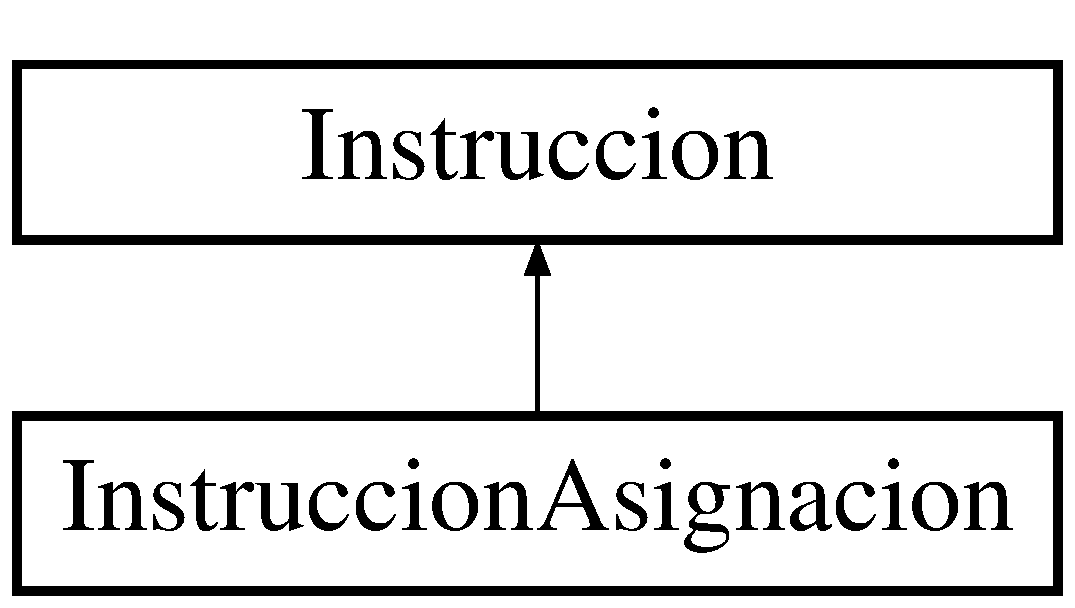
\includegraphics[height=2.000000cm]{class_instruccion_asignacion}
\end{center}
\end{figure}
\subsection*{Métodos públicos}
\begin{DoxyCompactItemize}
\item 
\hypertarget{class_instruccion_asignacion_a90f0375cdae6fa64adbd0c2aceb84414}{{\bfseries Instruccion\-Asignacion} (\hyperlink{class_expresion}{Expresion} $\ast$variable, \hyperlink{class_expresion}{Expresion} $\ast$expresion, \hyperlink{class_instruccion}{Instruccion} $\ast$siguiente, int id\-De\-Expresion, int numero\-De\-Linea)}\label{class_instruccion_asignacion_a90f0375cdae6fa64adbd0c2aceb84414}

\item 
\hypertarget{class_instruccion_asignacion_a998f9625b02d658d2bfc40de0f566fa9}{{\bfseries Instruccion\-Asignacion} (\hyperlink{class_variable_arreglo}{Variable\-Arreglo} $\ast$variable, \hyperlink{class_lista}{Lista} $\ast$lista\-Indices, \hyperlink{class_instruccion}{Instruccion} $\ast$siguiente, int id\-De\-Expresion, int numero\-De\-Linea)}\label{class_instruccion_asignacion_a998f9625b02d658d2bfc40de0f566fa9}

\item 
\hypertarget{class_instruccion_asignacion_a4d7d5963281b5f88540c17a2943fb42c}{virtual void {\bfseries validar\-Semantica} ()}\label{class_instruccion_asignacion_a4d7d5963281b5f88540c17a2943fb42c}

\item 
\hypertarget{class_instruccion_asignacion_a9adc3f513455df4e091e45beeaad373d}{virtual string {\bfseries generar\-Codigo\-Java} ()}\label{class_instruccion_asignacion_a9adc3f513455df4e091e45beeaad373d}

\item 
\hypertarget{class_instruccion_asignacion_a6ff32eb066888eac75245868ea8479f1}{\hyperlink{class_expresion}{Expresion} $\ast$ {\bfseries obtener\-Variable} ()}\label{class_instruccion_asignacion_a6ff32eb066888eac75245868ea8479f1}

\item 
\hypertarget{class_instruccion_asignacion_aa45f3254717e9723f00cae33c7bc295c}{\hyperlink{class_expresion}{Expresion} $\ast$ {\bfseries obtener\-Expresion} ()}\label{class_instruccion_asignacion_aa45f3254717e9723f00cae33c7bc295c}

\item 
\hypertarget{class_instruccion_asignacion_af2c792b744d63e163e249d8d4472f373}{string {\bfseries obtener\-Variable\-Con\-Id\-De\-Expresion} ()}\label{class_instruccion_asignacion_af2c792b744d63e163e249d8d4472f373}

\end{DoxyCompactItemize}
\subsection*{Otros miembros heredados}


La documentación para esta clase fue generada a partir de los siguientes ficheros\-:\begin{DoxyCompactItemize}
\item 
Instruccion/Instruccion\-Asignacion.\-h\item 
Instruccion/Instruccion\-Asignacion.\-cpp\end{DoxyCompactItemize}

\hypertarget{class_instruccion_asignacion_arreglo}{\section{Referencia de la Clase Instruccion\-Asignacion\-Arreglo}
\label{class_instruccion_asignacion_arreglo}\index{Instruccion\-Asignacion\-Arreglo@{Instruccion\-Asignacion\-Arreglo}}
}
Diagrama de herencias de Instruccion\-Asignacion\-Arreglo\begin{figure}[H]
\begin{center}
\leavevmode
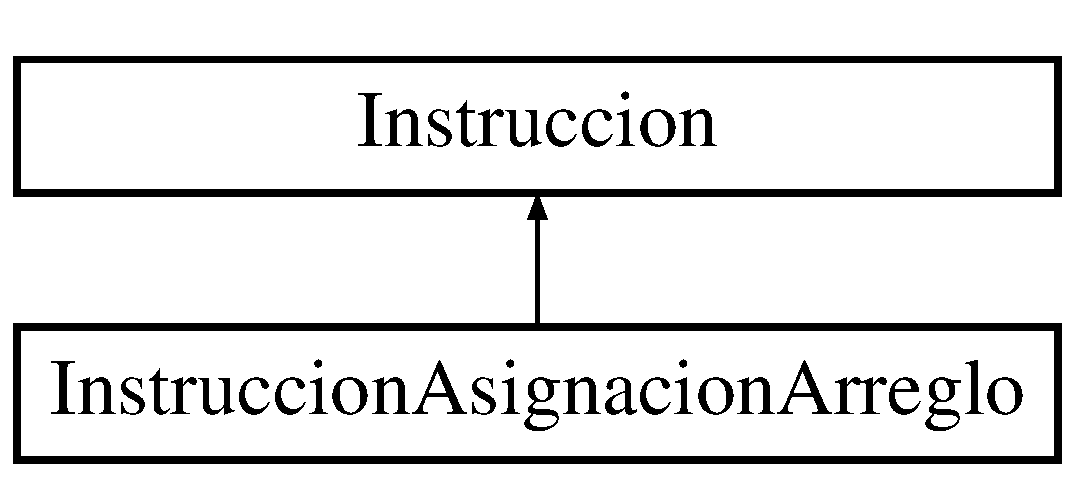
\includegraphics[height=2.000000cm]{class_instruccion_asignacion_arreglo}
\end{center}
\end{figure}
\subsection*{Métodos públicos}
\begin{DoxyCompactItemize}
\item 
\hypertarget{class_instruccion_asignacion_arreglo_a817cc80d03ef0bcc42c938ea56e13552}{{\bfseries Instruccion\-Asignacion\-Arreglo} (\hyperlink{class_variable_arreglo}{Variable\-Arreglo} $\ast$variable, \hyperlink{class_expresion}{Expresion} $\ast$expr, \hyperlink{class_instruccion}{Instruccion} $\ast$siguiente, int id\-De\-Expresion, int numero\-De\-Linea)}\label{class_instruccion_asignacion_arreglo_a817cc80d03ef0bcc42c938ea56e13552}

\item 
\hypertarget{class_instruccion_asignacion_arreglo_afc00f30c28ac29e2a20785ba0b0602de}{virtual void {\bfseries validar\-Semantica} ()}\label{class_instruccion_asignacion_arreglo_afc00f30c28ac29e2a20785ba0b0602de}

\item 
\hypertarget{class_instruccion_asignacion_arreglo_abb9cd8f5684dc856b7539c08cb190113}{virtual string {\bfseries generar\-Codigo\-Java} ()}\label{class_instruccion_asignacion_arreglo_abb9cd8f5684dc856b7539c08cb190113}

\end{DoxyCompactItemize}
\subsection*{Otros miembros heredados}


La documentación para esta clase fue generada a partir de los siguientes ficheros\-:\begin{DoxyCompactItemize}
\item 
Instruccion\-Asignacion\-Arreglo.\-h\item 
Instruccion\-Asignacion\-Arreglo.\-cpp\end{DoxyCompactItemize}

\hypertarget{class_instruccion_caso}{\section{Referencia de la Clase Instruccion\-Caso}
\label{class_instruccion_caso}\index{Instruccion\-Caso@{Instruccion\-Caso}}
}
Diagrama de herencias de Instruccion\-Caso\begin{figure}[H]
\begin{center}
\leavevmode
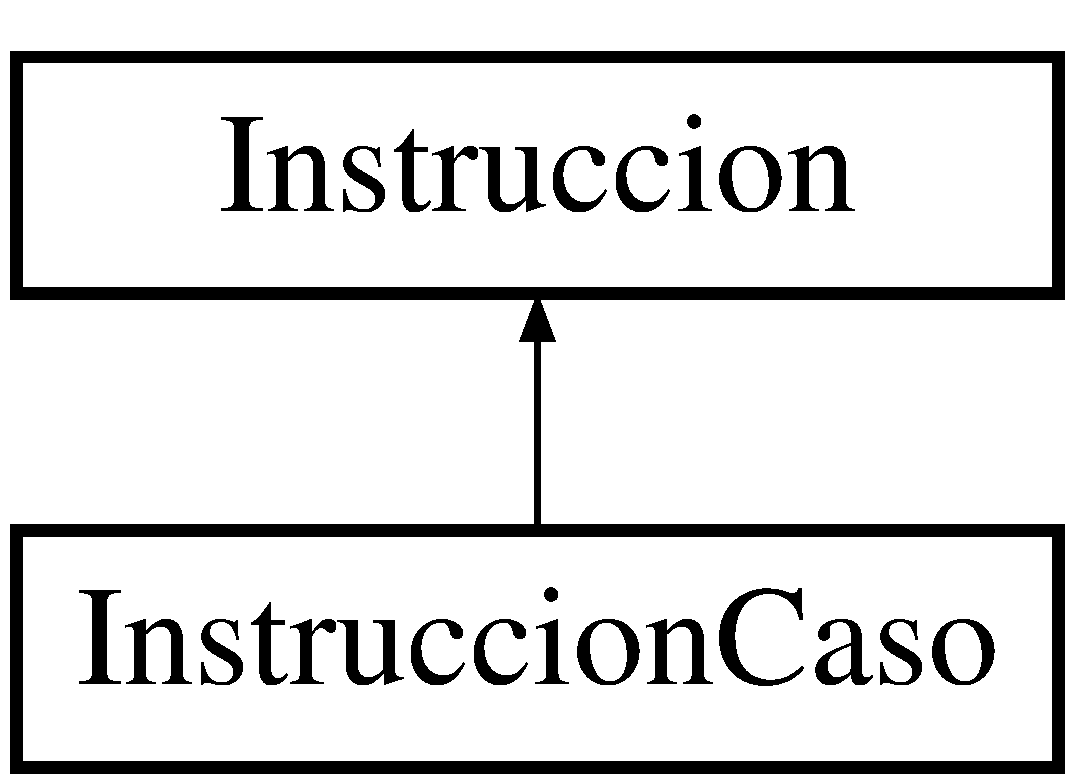
\includegraphics[height=2.000000cm]{class_instruccion_caso}
\end{center}
\end{figure}
\subsection*{Métodos públicos}
\begin{DoxyCompactItemize}
\item 
\hypertarget{class_instruccion_caso_a88695ac9095d9a47fa5320b14fa90fe1}{{\bfseries Instruccion\-Caso} (\hyperlink{class_expresion}{Expresion} $\ast$expresion, \hyperlink{class_lista_de_caso}{Lista\-De\-Caso} $\ast$lista\-De\-Caso, \hyperlink{class_instruccion}{Instruccion} $\ast$instrucciones\-\_\-sino, \hyperlink{class_instruccion}{Instruccion} $\ast$siguiente, int id\-De\-Expresion, int numero\-De\-Linea)}\label{class_instruccion_caso_a88695ac9095d9a47fa5320b14fa90fe1}

\item 
\hypertarget{class_instruccion_caso_a1cc6a7209dae143c54ae67d2dfab3c6d}{virtual void {\bfseries validar\-Semantica} ()}\label{class_instruccion_caso_a1cc6a7209dae143c54ae67d2dfab3c6d}

\item 
\hypertarget{class_instruccion_caso_a0b4516e2d9342f357f8877b6771c3b40}{virtual string {\bfseries generar\-Codigo\-Java} ()}\label{class_instruccion_caso_a0b4516e2d9342f357f8877b6771c3b40}

\end{DoxyCompactItemize}
\subsection*{Otros miembros heredados}


La documentación para esta clase fue generada a partir de los siguientes ficheros\-:\begin{DoxyCompactItemize}
\item 
Instruccion/Instruccion\-Caso.\-h\item 
Instruccion/Instruccion\-Caso.\-cpp\end{DoxyCompactItemize}

\hypertarget{class_instruccion_llamada_a_funcion}{\section{Referencia de la Clase Instruccion\-Llamada\-A\-Funcion}
\label{class_instruccion_llamada_a_funcion}\index{Instruccion\-Llamada\-A\-Funcion@{Instruccion\-Llamada\-A\-Funcion}}
}
Diagrama de herencias de Instruccion\-Llamada\-A\-Funcion\begin{figure}[H]
\begin{center}
\leavevmode
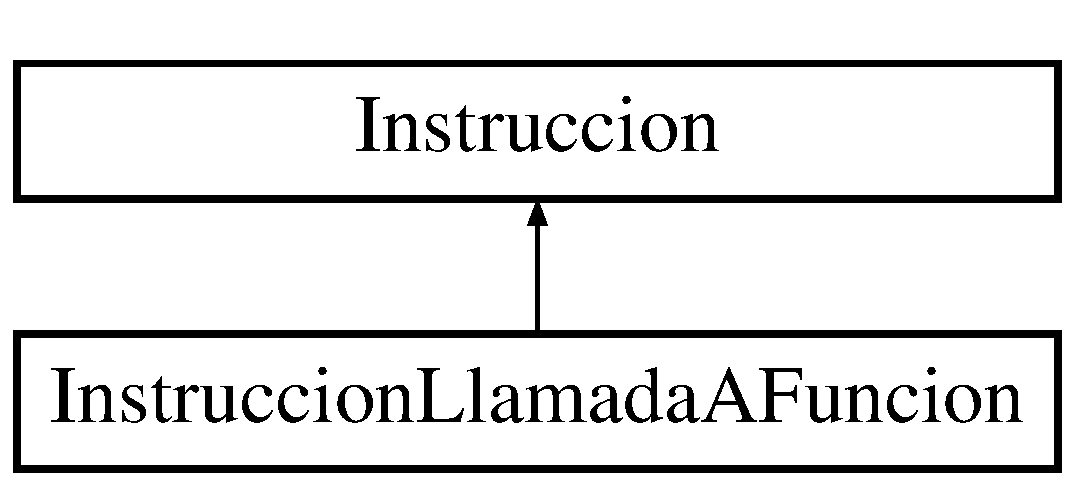
\includegraphics[height=2.000000cm]{class_instruccion_llamada_a_funcion}
\end{center}
\end{figure}
\subsection*{Métodos públicos}
\begin{DoxyCompactItemize}
\item 
\hypertarget{class_instruccion_llamada_a_funcion_abb47808f1a3ae5d218e3f02b899032f8}{{\bfseries Instruccion\-Llamada\-A\-Funcion} (string $\ast$identificador, \hyperlink{class_lista}{Lista} $\ast$lista\-\_\-parametros, \hyperlink{class_instruccion}{Instruccion} $\ast$siguiente, int id\-De\-Expresion, int numero\-De\-Linea)}\label{class_instruccion_llamada_a_funcion_abb47808f1a3ae5d218e3f02b899032f8}

\item 
\hypertarget{class_instruccion_llamada_a_funcion_a8d10eb990d87092020c7b7cb3f7961a1}{virtual void {\bfseries validar\-Semantica} ()}\label{class_instruccion_llamada_a_funcion_a8d10eb990d87092020c7b7cb3f7961a1}

\item 
\hypertarget{class_instruccion_llamada_a_funcion_aa48f82d3daf3d97c2e9a855609df7ac7}{virtual string {\bfseries generar\-Codigo\-Java} ()}\label{class_instruccion_llamada_a_funcion_aa48f82d3daf3d97c2e9a855609df7ac7}

\end{DoxyCompactItemize}
\subsection*{Otros miembros heredados}


La documentación para esta clase fue generada a partir de los siguientes ficheros\-:\begin{DoxyCompactItemize}
\item 
Instruccion/Instruccion\-Llamada\-A\-Funcion.\-h\item 
Instruccion/Instruccion\-Llamada\-A\-Funcion.\-cpp\end{DoxyCompactItemize}

\hypertarget{class_instruccion_mientras}{\section{Referencia de la Clase Instruccion\-Mientras}
\label{class_instruccion_mientras}\index{Instruccion\-Mientras@{Instruccion\-Mientras}}
}
Diagrama de herencias de Instruccion\-Mientras\begin{figure}[H]
\begin{center}
\leavevmode
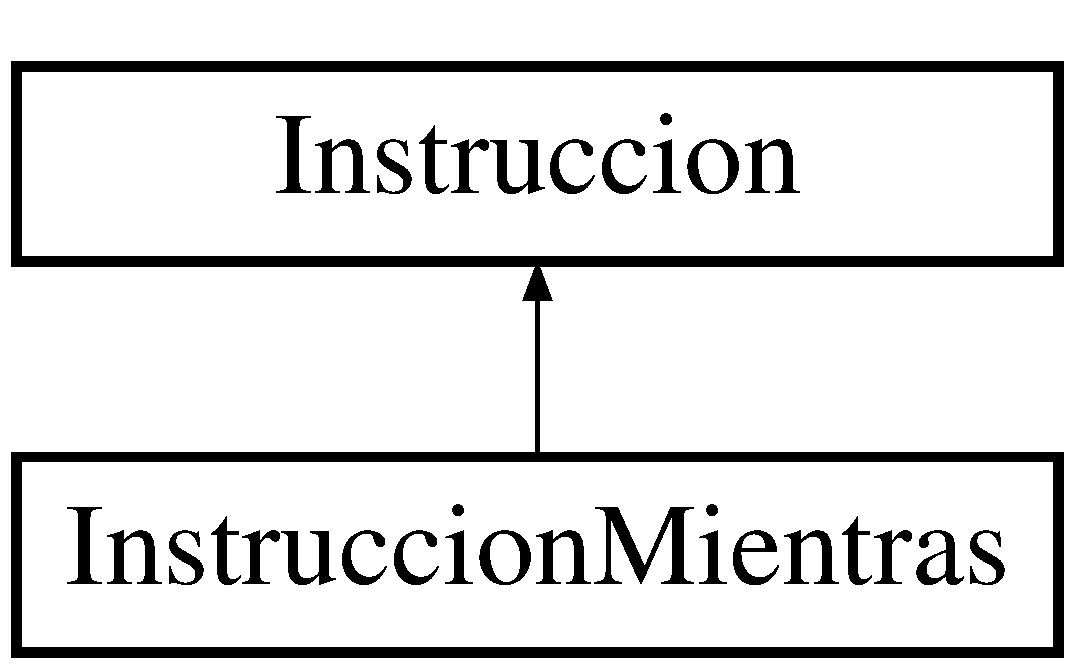
\includegraphics[height=2.000000cm]{class_instruccion_mientras}
\end{center}
\end{figure}
\subsection*{Métodos públicos}
\begin{DoxyCompactItemize}
\item 
\hypertarget{class_instruccion_mientras_a7440d7d6b174efc017dbabdca59c3374}{{\bfseries Instruccion\-Mientras} (\hyperlink{class_expresion}{Expresion} $\ast$condicion, \hyperlink{class_instruccion}{Instruccion} $\ast$instrucciones, \hyperlink{class_instruccion}{Instruccion} $\ast$siguiente, int id\-De\-Expresion, int numero\-De\-Linea)}\label{class_instruccion_mientras_a7440d7d6b174efc017dbabdca59c3374}

\item 
\hypertarget{class_instruccion_mientras_a3f84acd2d81b1fde00dd0c5aafb07503}{virtual void {\bfseries validar\-Semantica} ()}\label{class_instruccion_mientras_a3f84acd2d81b1fde00dd0c5aafb07503}

\item 
\hypertarget{class_instruccion_mientras_afb7d0018cd8f162d117fdab2d3241be6}{virtual string {\bfseries generar\-Codigo\-Java} ()}\label{class_instruccion_mientras_afb7d0018cd8f162d117fdab2d3241be6}

\end{DoxyCompactItemize}
\subsection*{Otros miembros heredados}


La documentación para esta clase fue generada a partir de los siguientes ficheros\-:\begin{DoxyCompactItemize}
\item 
Instruccion/Instruccion\-Mientras.\-h\item 
Instruccion/Instruccion\-Mientras.\-cpp\end{DoxyCompactItemize}

\hypertarget{class_instruccion_para}{\section{Referencia de la Clase Instruccion\-Para}
\label{class_instruccion_para}\index{Instruccion\-Para@{Instruccion\-Para}}
}
Diagrama de herencias de Instruccion\-Para\begin{figure}[H]
\begin{center}
\leavevmode
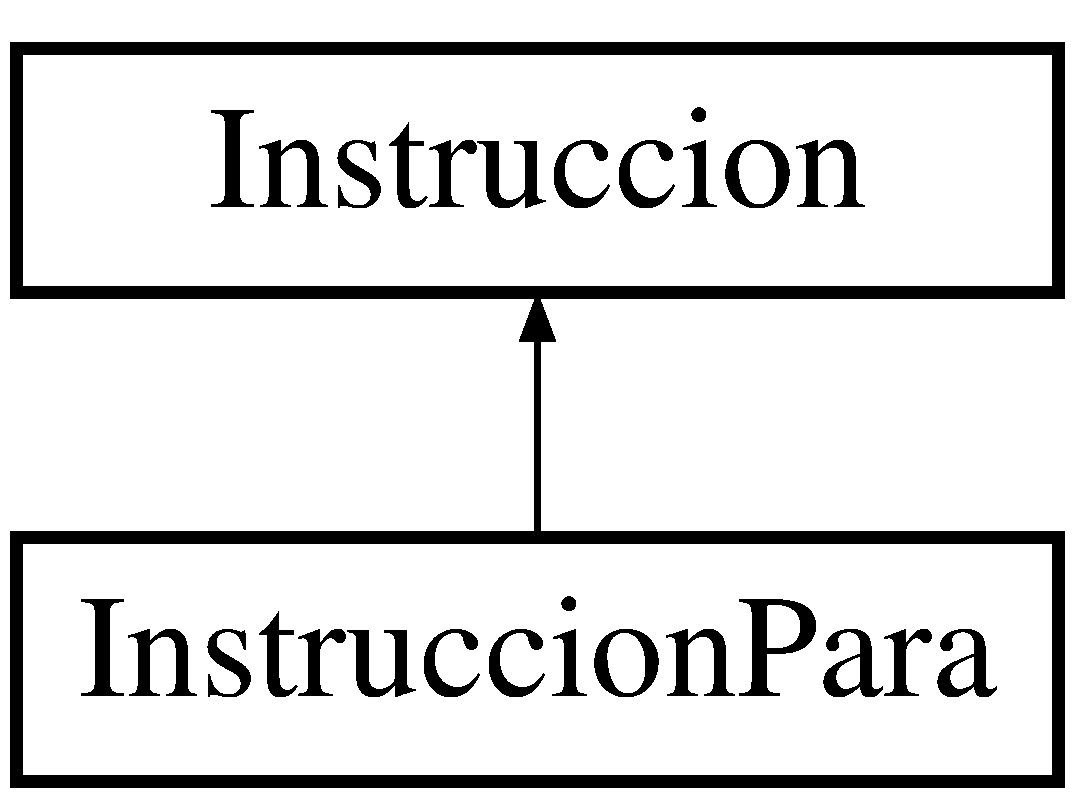
\includegraphics[height=2.000000cm]{class_instruccion_para}
\end{center}
\end{figure}
\subsection*{Métodos públicos}
\begin{DoxyCompactItemize}
\item 
\hypertarget{class_instruccion_para_ab17f0a2666c007f8628e64e2e9565706}{{\bfseries Instruccion\-Para} (\hyperlink{class_instruccion_asignacion}{Instruccion\-Asignacion} $\ast$instruccion\-Asignacion, \hyperlink{class_expresion}{Expresion} $\ast$final, \hyperlink{class_instruccion}{Instruccion} $\ast$instrucciones, \hyperlink{class_instruccion}{Instruccion} $\ast$siguiente, int id\-De\-Expresion, int numero\-De\-Linea)}\label{class_instruccion_para_ab17f0a2666c007f8628e64e2e9565706}

\item 
\hypertarget{class_instruccion_para_aa33221010c58fa12a4bd0ef8326e61cd}{virtual void {\bfseries validar\-Semantica} ()}\label{class_instruccion_para_aa33221010c58fa12a4bd0ef8326e61cd}

\item 
\hypertarget{class_instruccion_para_a793b98134eef15c55703fc4183c196b3}{virtual string {\bfseries generar\-Codigo\-Java} ()}\label{class_instruccion_para_a793b98134eef15c55703fc4183c196b3}

\end{DoxyCompactItemize}
\subsection*{Otros miembros heredados}


La documentación para esta clase fue generada a partir de los siguientes ficheros\-:\begin{DoxyCompactItemize}
\item 
Instruccion/Instruccion\-Para.\-h\item 
Instruccion/Instruccion\-Para.\-cpp\end{DoxyCompactItemize}

\hypertarget{class_instruccion_para_cada}{\section{Referencia de la Clase Instruccion\-Para\-Cada}
\label{class_instruccion_para_cada}\index{Instruccion\-Para\-Cada@{Instruccion\-Para\-Cada}}
}
Diagrama de herencias de Instruccion\-Para\-Cada\begin{figure}[H]
\begin{center}
\leavevmode
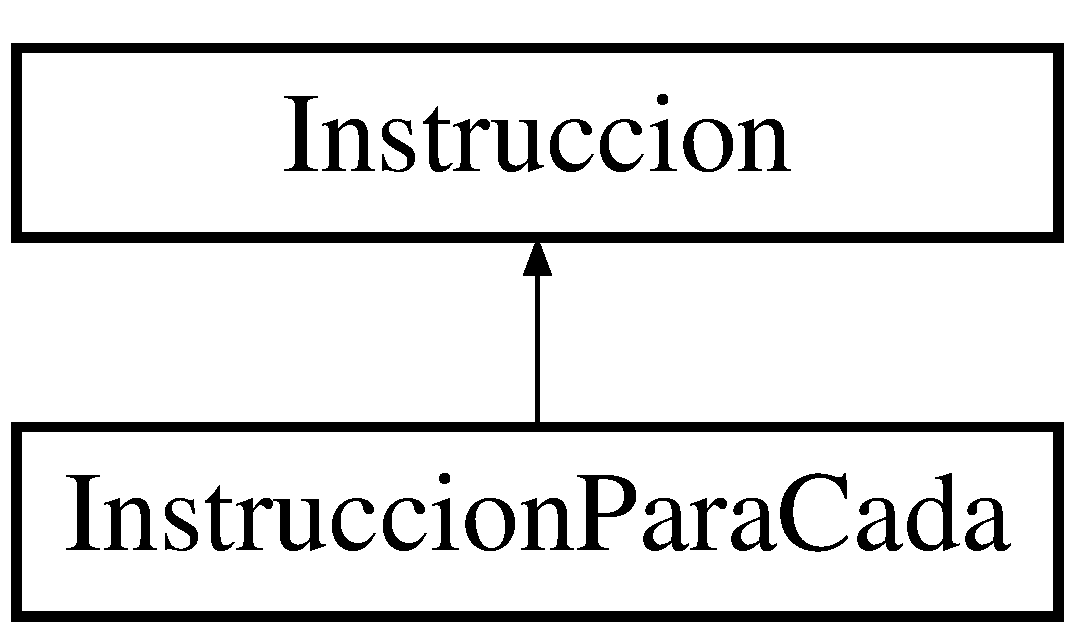
\includegraphics[height=2.000000cm]{class_instruccion_para_cada}
\end{center}
\end{figure}
\subsection*{Métodos públicos}
\begin{DoxyCompactItemize}
\item 
\hypertarget{class_instruccion_para_cada_aa7a2b691820b92de13a7c9bc2a0769d0}{{\bfseries Instruccion\-Para\-Cada} (\hyperlink{class_expresion}{Expresion} $\ast$variable, \hyperlink{class_expresion}{Expresion} $\ast$coleccion\-\_\-arreglo, \hyperlink{class_instruccion}{Instruccion} $\ast$instrucciones, \hyperlink{class_instruccion}{Instruccion} $\ast$siguiente, int id\-De\-Expresion, int numero\-De\-Linea)}\label{class_instruccion_para_cada_aa7a2b691820b92de13a7c9bc2a0769d0}

\item 
\hypertarget{class_instruccion_para_cada_a177a6b78748dfd96139f00e2ad417ec1}{virtual void {\bfseries validar\-Semantica} ()}\label{class_instruccion_para_cada_a177a6b78748dfd96139f00e2ad417ec1}

\item 
\hypertarget{class_instruccion_para_cada_ade8876617a19596c63281c0f36f01155}{virtual string {\bfseries generar\-Codigo\-Java} ()}\label{class_instruccion_para_cada_ade8876617a19596c63281c0f36f01155}

\end{DoxyCompactItemize}
\subsection*{Otros miembros heredados}


La documentación para esta clase fue generada a partir de los siguientes ficheros\-:\begin{DoxyCompactItemize}
\item 
Instruccion/Instruccion\-Para\-Cada.\-h\item 
Instruccion/Instruccion\-Para\-Cada.\-cpp\end{DoxyCompactItemize}

\hypertarget{class_instruccion_repetir}{\section{Referencia de la Clase Instruccion\-Repetir}
\label{class_instruccion_repetir}\index{Instruccion\-Repetir@{Instruccion\-Repetir}}
}
Diagrama de herencias de Instruccion\-Repetir\begin{figure}[H]
\begin{center}
\leavevmode
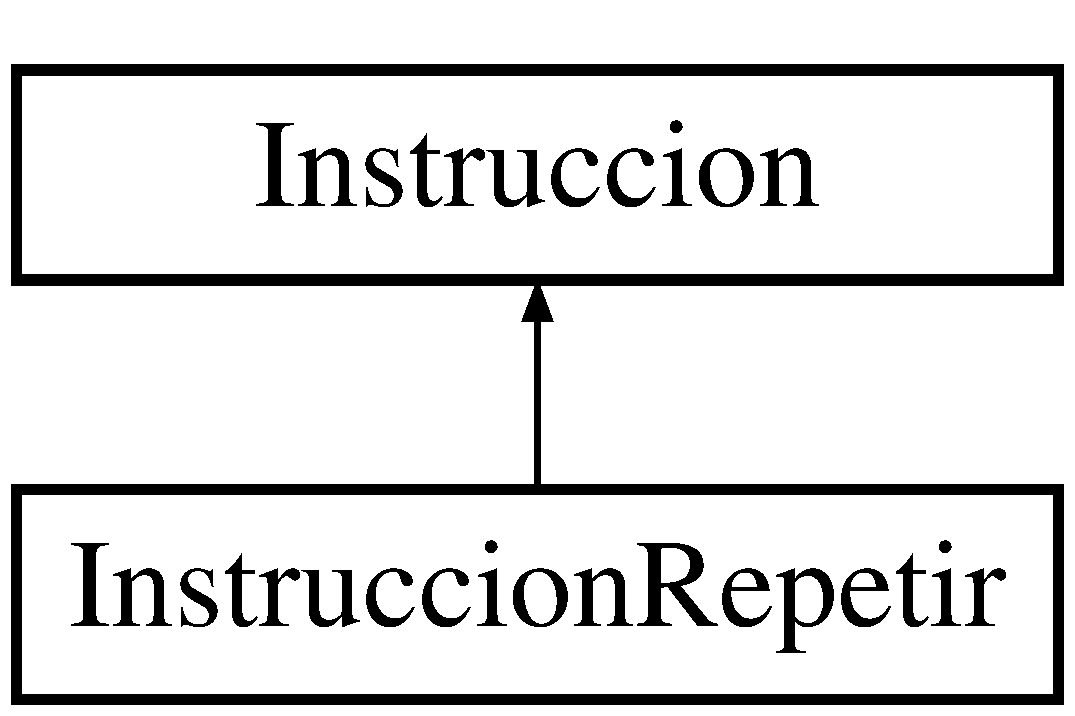
\includegraphics[height=2.000000cm]{class_instruccion_repetir}
\end{center}
\end{figure}
\subsection*{Métodos públicos}
\begin{DoxyCompactItemize}
\item 
\hypertarget{class_instruccion_repetir_a875f3bae2adb85cacb6cc44544fb9723}{{\bfseries Instruccion\-Repetir} (\hyperlink{class_expresion}{Expresion} $\ast$cantidad, \hyperlink{class_instruccion}{Instruccion} $\ast$instrucciones, \hyperlink{class_instruccion}{Instruccion} $\ast$siguiente, int id\-De\-Expresion, int numero\-De\-Linea)}\label{class_instruccion_repetir_a875f3bae2adb85cacb6cc44544fb9723}

\item 
\hypertarget{class_instruccion_repetir_aa5481045a63c0b8d291906cf9ff447ec}{virtual void {\bfseries validar\-Semantica} ()}\label{class_instruccion_repetir_aa5481045a63c0b8d291906cf9ff447ec}

\item 
\hypertarget{class_instruccion_repetir_a3eb806856e86707007b5578eba019545}{virtual string {\bfseries generar\-Codigo\-Java} ()}\label{class_instruccion_repetir_a3eb806856e86707007b5578eba019545}

\end{DoxyCompactItemize}
\subsection*{Otros miembros heredados}


La documentación para esta clase fue generada a partir de los siguientes ficheros\-:\begin{DoxyCompactItemize}
\item 
Instruccion/Instruccion\-Repetir.\-h\item 
Instruccion/Instruccion\-Repetir.\-cpp\end{DoxyCompactItemize}

\hypertarget{class_instruccion_repita}{\section{Referencia de la Clase Instruccion\-Repita}
\label{class_instruccion_repita}\index{Instruccion\-Repita@{Instruccion\-Repita}}
}
Diagrama de herencias de Instruccion\-Repita\begin{figure}[H]
\begin{center}
\leavevmode
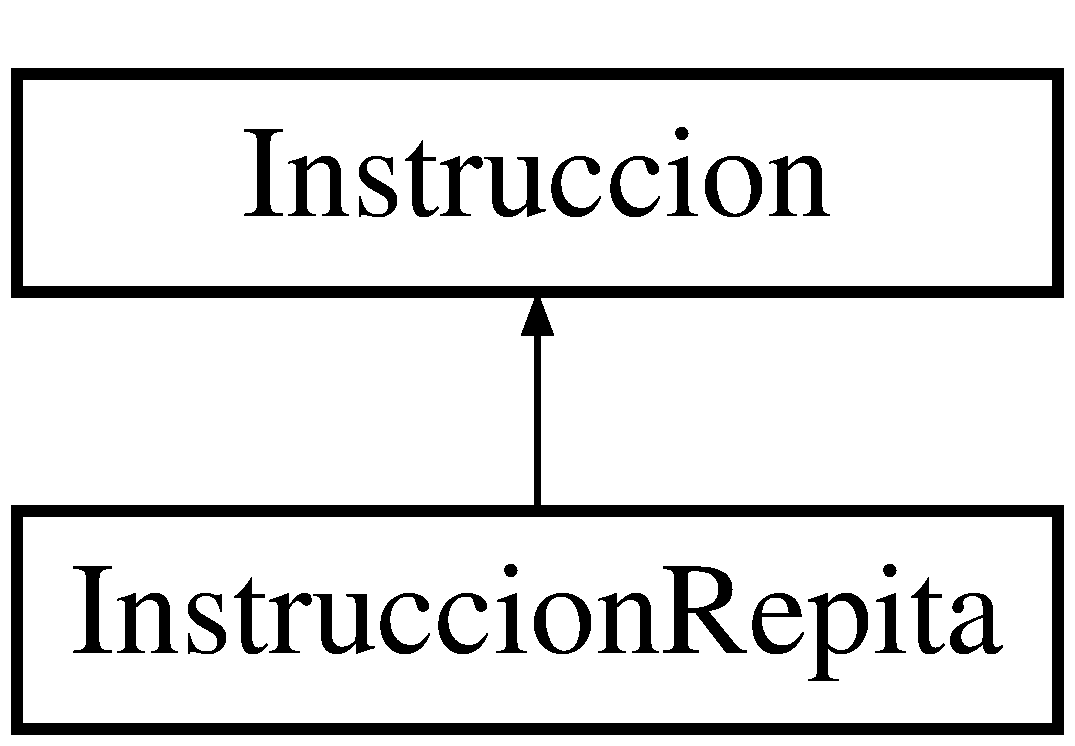
\includegraphics[height=2.000000cm]{class_instruccion_repita}
\end{center}
\end{figure}
\subsection*{Métodos públicos}
\begin{DoxyCompactItemize}
\item 
\hypertarget{class_instruccion_repita_a754302f91716408b5ee445442cf26549}{{\bfseries Instruccion\-Repita} (\hyperlink{class_expresion}{Expresion} $\ast$condicion, \hyperlink{class_instruccion}{Instruccion} $\ast$siguiente, int id\-De\-Expresion, int numero\-De\-Linea)}\label{class_instruccion_repita_a754302f91716408b5ee445442cf26549}

\item 
\hypertarget{class_instruccion_repita_ae1b3075c328d3fef683d75a54dfe5b17}{virtual void {\bfseries validar\-Semantica} ()}\label{class_instruccion_repita_ae1b3075c328d3fef683d75a54dfe5b17}

\item 
\hypertarget{class_instruccion_repita_a6d23140f918de6995d69e7d5a3b911f4}{\hyperlink{class_expresion}{Expresion} $\ast$ {\bfseries obtener\-Condicion} ()}\label{class_instruccion_repita_a6d23140f918de6995d69e7d5a3b911f4}

\item 
\hypertarget{class_instruccion_repita_a350f2db05e5af509869a5012cb0eab2c}{virtual string {\bfseries generar\-Codigo\-Java} ()}\label{class_instruccion_repita_a350f2db05e5af509869a5012cb0eab2c}

\end{DoxyCompactItemize}
\subsection*{Otros miembros heredados}


La documentación para esta clase fue generada a partir de los siguientes ficheros\-:\begin{DoxyCompactItemize}
\item 
Instruccion/Instruccion\-Repita.\-h\item 
Instruccion/Instruccion\-Repita.\-cpp\end{DoxyCompactItemize}

\hypertarget{class_instruccion_repita_desde}{\section{Referencia de la Clase Instruccion\-Repita\-Desde}
\label{class_instruccion_repita_desde}\index{Instruccion\-Repita\-Desde@{Instruccion\-Repita\-Desde}}
}
Diagrama de herencias de Instruccion\-Repita\-Desde\begin{figure}[H]
\begin{center}
\leavevmode
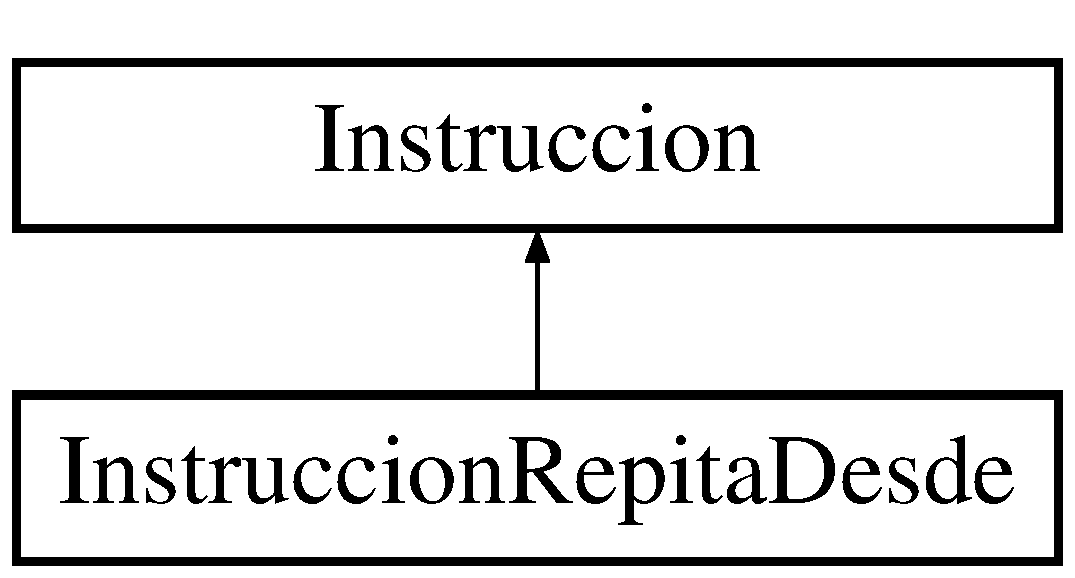
\includegraphics[height=2.000000cm]{class_instruccion_repita_desde}
\end{center}
\end{figure}
\subsection*{Métodos públicos}
\begin{DoxyCompactItemize}
\item 
\hypertarget{class_instruccion_repita_desde_af26800cd1eb9f21b41b91c57927cd582}{{\bfseries Instruccion\-Repita\-Desde} (\hyperlink{class_expresion}{Expresion} $\ast$inicio, \hyperlink{class_expresion}{Expresion} $\ast$final, \hyperlink{class_instruccion}{Instruccion} $\ast$instrucciones, \hyperlink{class_instruccion}{Instruccion} $\ast$siguiente, int id\-De\-Expresion, int numero\-De\-Linea)}\label{class_instruccion_repita_desde_af26800cd1eb9f21b41b91c57927cd582}

\item 
\hypertarget{class_instruccion_repita_desde_af4405f4e81b9bc73d27623c68c096ce5}{virtual void {\bfseries validar\-Semantica} ()}\label{class_instruccion_repita_desde_af4405f4e81b9bc73d27623c68c096ce5}

\item 
\hypertarget{class_instruccion_repita_desde_acd4ade3e3b7a86f242ec87401fe4cd1f}{virtual string {\bfseries generar\-Codigo\-Java} ()}\label{class_instruccion_repita_desde_acd4ade3e3b7a86f242ec87401fe4cd1f}

\end{DoxyCompactItemize}
\subsection*{Otros miembros heredados}


La documentación para esta clase fue generada a partir de los siguientes ficheros\-:\begin{DoxyCompactItemize}
\item 
Instruccion/Instruccion\-Repita\-Desde.\-h\item 
Instruccion/Instruccion\-Repita\-Desde.\-cpp\end{DoxyCompactItemize}

\hypertarget{class_instruccion_retornar}{\section{Referencia de la Clase Instruccion\-Retornar}
\label{class_instruccion_retornar}\index{Instruccion\-Retornar@{Instruccion\-Retornar}}
}
Diagrama de herencias de Instruccion\-Retornar\begin{figure}[H]
\begin{center}
\leavevmode
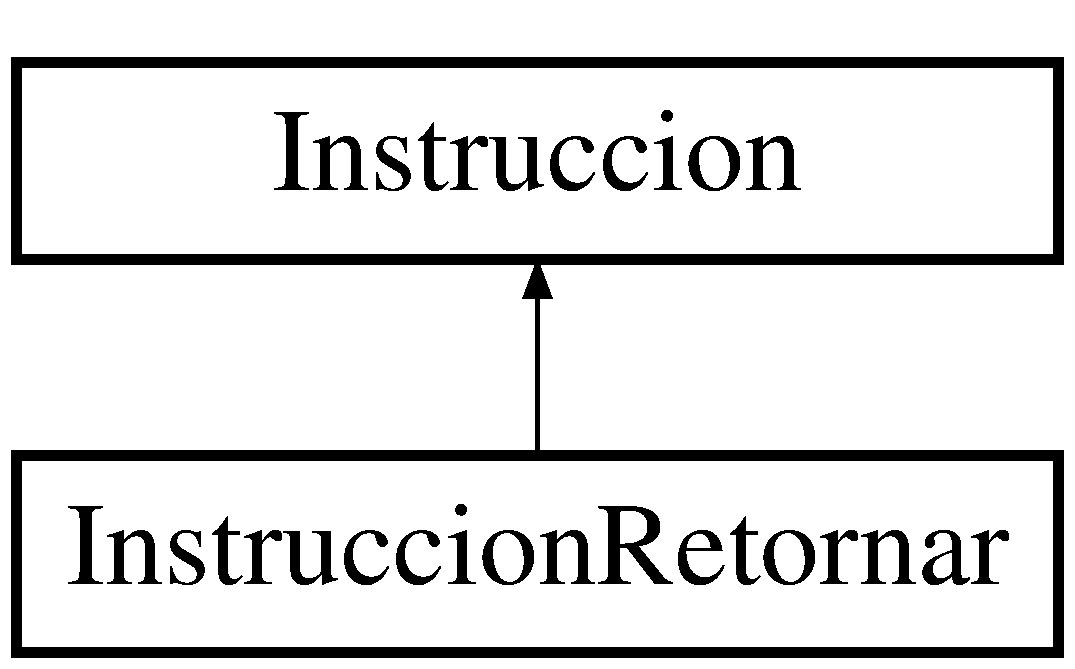
\includegraphics[height=2.000000cm]{class_instruccion_retornar}
\end{center}
\end{figure}
\subsection*{Métodos públicos}
\begin{DoxyCompactItemize}
\item 
\hypertarget{class_instruccion_retornar_a5dedcbb7284963865a14c6404ce611e6}{{\bfseries Instruccion\-Retornar} (\hyperlink{class_expresion}{Expresion} $\ast$expresion\-\_\-de\-\_\-retorno, \hyperlink{class_instruccion}{Instruccion} $\ast$siguiente, int id\-De\-Expresion, int numero\-De\-Linea)}\label{class_instruccion_retornar_a5dedcbb7284963865a14c6404ce611e6}

\item 
\hypertarget{class_instruccion_retornar_a851f2b2dbef7e7d26ff7e3c0d1838150}{virtual void {\bfseries validar\-Semantica} ()}\label{class_instruccion_retornar_a851f2b2dbef7e7d26ff7e3c0d1838150}

\item 
\hypertarget{class_instruccion_retornar_a61048d7238b2c5f285e75e506dd1a1ef}{virtual string {\bfseries generar\-Codigo\-Java} ()}\label{class_instruccion_retornar_a61048d7238b2c5f285e75e506dd1a1ef}

\item 
\hypertarget{class_instruccion_retornar_af805d72620a9db7a3fc749a2ba414cff}{void {\bfseries establecer\-Tipo\-De\-Retorno} (\hyperlink{class_tipo}{Tipo} $\ast$tipo\-De\-Retorno)}\label{class_instruccion_retornar_af805d72620a9db7a3fc749a2ba414cff}

\item 
\hypertarget{class_instruccion_retornar_ab6f78cf720f50134dca62f385d35c3ad}{\hyperlink{class_tipo}{Tipo} $\ast$ {\bfseries obtener\-Tipo\-De\-Retorno} ()}\label{class_instruccion_retornar_ab6f78cf720f50134dca62f385d35c3ad}

\end{DoxyCompactItemize}
\subsection*{Otros miembros heredados}


La documentación para esta clase fue generada a partir de los siguientes ficheros\-:\begin{DoxyCompactItemize}
\item 
Instruccion/Instruccion\-Retornar.\-h\item 
Instruccion/Instruccion\-Retornar.\-cpp\end{DoxyCompactItemize}

\hypertarget{class_instruccion_si}{\section{Referencia de la Clase Instruccion\-Si}
\label{class_instruccion_si}\index{Instruccion\-Si@{Instruccion\-Si}}
}
Diagrama de herencias de Instruccion\-Si\begin{figure}[H]
\begin{center}
\leavevmode
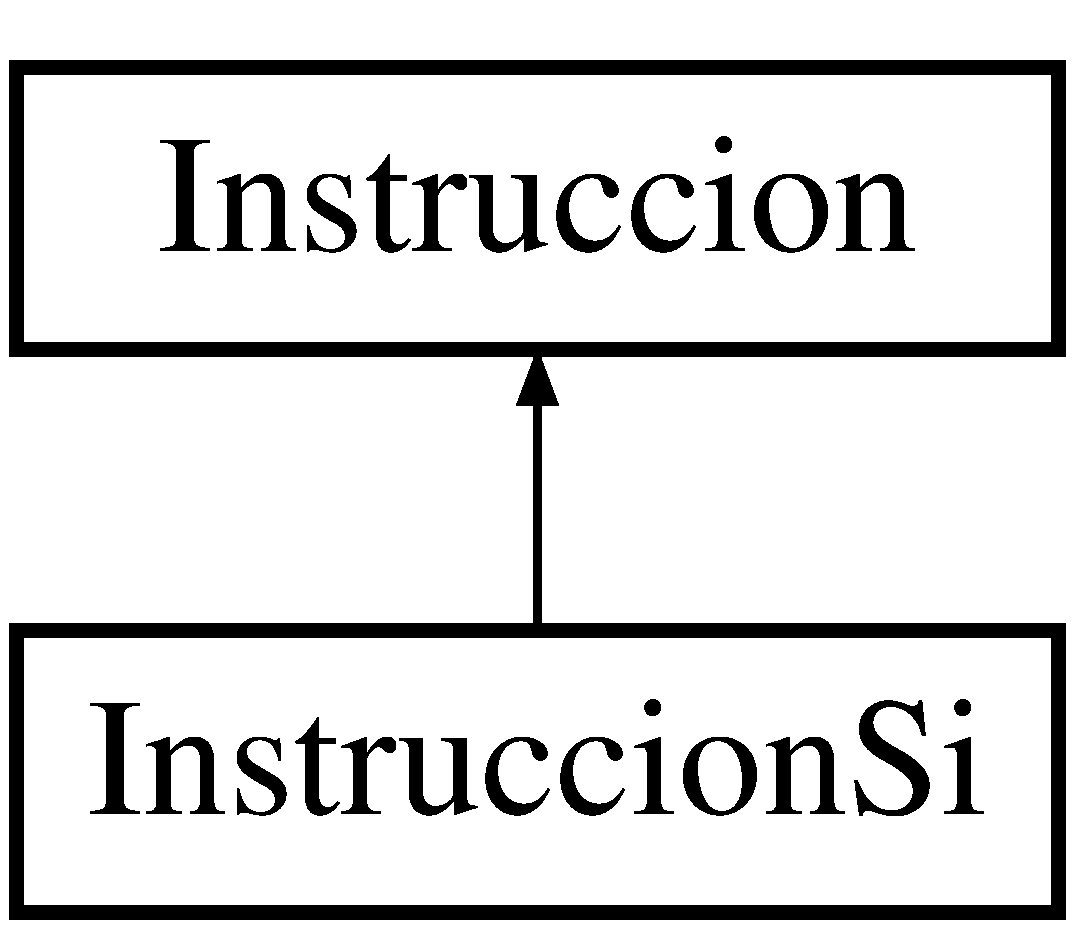
\includegraphics[height=2.000000cm]{class_instruccion_si}
\end{center}
\end{figure}
\subsection*{Métodos públicos}
\begin{DoxyCompactItemize}
\item 
\hypertarget{class_instruccion_si_ace01e331a65f23e90b422e435975d074}{{\bfseries Instruccion\-Si} (\hyperlink{class_expresion}{Expresion} $\ast$condicion, \hyperlink{class_instruccion}{Instruccion} $\ast$instrucciones\-Si\-Verdadero, \hyperlink{class_instruccion}{Instruccion} $\ast$instrucciones\-Si\-Falso, \hyperlink{class_instruccion}{Instruccion} $\ast$instruccion\-Si\-Anidado, \hyperlink{class_instruccion}{Instruccion} $\ast$siguiente, int id\-De\-Expresion, int numero\-De\-Linea)}\label{class_instruccion_si_ace01e331a65f23e90b422e435975d074}

\item 
\hypertarget{class_instruccion_si_a926b9ce81a71ee3ba8ccc43a9324f62a}{virtual void {\bfseries validar\-Semantica} ()}\label{class_instruccion_si_a926b9ce81a71ee3ba8ccc43a9324f62a}

\item 
\hypertarget{class_instruccion_si_a4db7a3a6d7141b29a507d42b010ee596}{virtual string {\bfseries generar\-Codigo\-Java} ()}\label{class_instruccion_si_a4db7a3a6d7141b29a507d42b010ee596}

\end{DoxyCompactItemize}
\subsection*{Otros miembros heredados}


La documentación para esta clase fue generada a partir de los siguientes ficheros\-:\begin{DoxyCompactItemize}
\item 
Instruccion/Instruccion\-Si.\-h\item 
Instruccion/Instruccion\-Si.\-cpp\end{DoxyCompactItemize}

\hypertarget{class_lista}{\section{Referencia de la Clase Lista}
\label{class_lista}\index{Lista@{Lista}}
}
\subsection*{Atributos públicos}
\begin{DoxyCompactItemize}
\item 
\hypertarget{class_lista_ab717ea9786ada3e085c9e7c64a362cc3}{vector$<$ \hyperlink{class_expresion}{Expresion} $\ast$ $>$ $\ast$ {\bfseries lista}}\label{class_lista_ab717ea9786ada3e085c9e7c64a362cc3}

\end{DoxyCompactItemize}


La documentación para esta clase fue generada a partir de los siguientes ficheros\-:\begin{DoxyCompactItemize}
\item 
Bison\-\_\-\-Flex/Lista.\-h\item 
Bison\-\_\-\-Flex/Lista.\-cpp\end{DoxyCompactItemize}

\hypertarget{class_lista_de_caso}{\section{Referencia de la Clase Lista\-De\-Caso}
\label{class_lista_de_caso}\index{Lista\-De\-Caso@{Lista\-De\-Caso}}
}
\subsection*{Métodos públicos}
\begin{DoxyCompactItemize}
\item 
\hypertarget{class_lista_de_caso_a4c4ec9e45d5a4d218795a65fe3afb35d}{{\bfseries Lista\-De\-Caso} (\hyperlink{class_expresion}{Expresion} $\ast$expresion\-\_\-caso, \hyperlink{class_instruccion}{Instruccion} $\ast$instrucciones, \hyperlink{class_lista_de_caso}{Lista\-De\-Caso} $\ast$siguiente)}\label{class_lista_de_caso_a4c4ec9e45d5a4d218795a65fe3afb35d}

\item 
\hypertarget{class_lista_de_caso_a9c6f0e007b19ce9f78be90af19a721a5}{void {\bfseries establecer\-Siguiente} (\hyperlink{class_lista_de_caso}{Lista\-De\-Caso} $\ast$siguiente)}\label{class_lista_de_caso_a9c6f0e007b19ce9f78be90af19a721a5}

\item 
\hypertarget{class_lista_de_caso_a09a6d396f80986bdab579b450ed5b59a}{\hyperlink{class_lista_de_caso}{Lista\-De\-Caso} $\ast$ {\bfseries obtener\-Siguiente} ()}\label{class_lista_de_caso_a09a6d396f80986bdab579b450ed5b59a}

\item 
\hypertarget{class_lista_de_caso_af5a5edca34cef6d795891a1e06c47731}{\hyperlink{class_expresion}{Expresion} $\ast$ {\bfseries obtener\-Expresion} ()}\label{class_lista_de_caso_af5a5edca34cef6d795891a1e06c47731}

\item 
\hypertarget{class_lista_de_caso_abe3ca7dd4a4589ce04201a0546d97888}{\hyperlink{class_instruccion}{Instruccion} $\ast$ {\bfseries obtener\-Instruccion} ()}\label{class_lista_de_caso_abe3ca7dd4a4589ce04201a0546d97888}

\end{DoxyCompactItemize}


La documentación para esta clase fue generada a partir de los siguientes ficheros\-:\begin{DoxyCompactItemize}
\item 
Instruccion/Lista\-De\-Caso.\-h\item 
Instruccion/Lista\-De\-Caso.\-cpp\end{DoxyCompactItemize}

\hypertarget{class_programa}{\section{Referencia de la Clase Programa}
\label{class_programa}\index{Programa@{Programa}}
}
\subsection*{Métodos públicos}
\begin{DoxyCompactItemize}
\item 
\hypertarget{class_programa_af659ea1395508d314d38ae9e4a1810c8}{void {\bfseries actualizar\-Variable\-Arreglo} (\hyperlink{class_variable_arreglo}{Variable\-Arreglo} $\ast$var)}\label{class_programa_af659ea1395508d314d38ae9e4a1810c8}

\item 
\hypertarget{class_programa_adcc8d19595a93cd41e5148589ef4600b}{void {\bfseries eliminar\-Tabla\-Variables\-Funcs\-Locales} ()}\label{class_programa_adcc8d19595a93cd41e5148589ef4600b}

\item 
\hypertarget{class_programa_a3365cc53aa7a733b8d9d99c813f6c897}{void {\bfseries establecer\-Tabla\-Variables\-Funcs\-Locales} (\hyperlink{class_lista}{Lista} $\ast$parametros, \hyperlink{class_lista}{Lista} $\ast$p2)}\label{class_programa_a3365cc53aa7a733b8d9d99c813f6c897}

\item 
\hypertarget{class_programa_acf9e779a8265278fb90d9cb9c4f1d4a6}{\hyperlink{class_variable_declarada}{Variable\-Declarada} $\ast$ {\bfseries obtener\-V\-Declarada\-Variables\-Funcs\-Locales} (string $\ast$)}\label{class_programa_acf9e779a8265278fb90d9cb9c4f1d4a6}

\item 
\hypertarget{class_programa_ab6b962e2bab0340f2a30de99c22dc19d}{string {\bfseries obtener\-Codigo\-Sensores\-Declarados} ()}\label{class_programa_ab6b962e2bab0340f2a30de99c22dc19d}

\item 
\hypertarget{class_programa_af4d3ed3f28acf78aff460031d53f4b74}{string {\bfseries obtener\-Codigo\-Variables\-A\-Declarar} ()}\label{class_programa_af4d3ed3f28acf78aff460031d53f4b74}

\item 
\hypertarget{class_programa_ae19984e7598f4faa075ebf48fa818596}{\hyperlink{class_tipo_booleano}{Tipo\-Booleano} $\ast$ {\bfseries obtener\-Tipo\-Booleano} ()}\label{class_programa_ae19984e7598f4faa075ebf48fa818596}

\item 
\hypertarget{class_programa_a18ee9edc7aea094f46ab06d21d5165f6}{\hyperlink{class_tipo_cadena}{Tipo\-Cadena} $\ast$ {\bfseries obtener\-Tipo\-Cadena} ()}\label{class_programa_a18ee9edc7aea094f46ab06d21d5165f6}

\item 
\hypertarget{class_programa_acd3b8c83b9ced2b2696ef3ba34b192b0}{\hyperlink{class_tipo_caracter}{Tipo\-Caracter} $\ast$ {\bfseries obtener\-Tipo\-Caracter} ()}\label{class_programa_acd3b8c83b9ced2b2696ef3ba34b192b0}

\item 
\hypertarget{class_programa_a2ca63877d33fc48a57995161267c9851}{\hyperlink{class_tipo_entero}{Tipo\-Entero} $\ast$ {\bfseries obtener\-Tipo\-Entero} ()}\label{class_programa_a2ca63877d33fc48a57995161267c9851}

\item 
\hypertarget{class_programa_a3b90b9472e6d0d9e4d2db36dcfa73bf8}{\hyperlink{class_tipo_flotante}{Tipo\-Flotante} $\ast$ {\bfseries obtener\-Tipo\-Flotante} ()}\label{class_programa_a3b90b9472e6d0d9e4d2db36dcfa73bf8}

\item 
\hypertarget{class_programa_a5fe10e53575d9d5df48b5f149e4f72cf}{\hyperlink{class_tipo_arreglo}{Tipo\-Arreglo} $\ast$ {\bfseries obtener\-Tipo\-Arreglo} ()}\label{class_programa_a5fe10e53575d9d5df48b5f149e4f72cf}

\item 
\hypertarget{class_programa_ab0fd5f510088ab0a0175a87948796c19}{\hyperlink{class_tipo_motor}{Tipo\-Motor} $\ast$ {\bfseries obtener\-Tipo\-Motor} ()}\label{class_programa_ab0fd5f510088ab0a0175a87948796c19}

\item 
\hypertarget{class_programa_ab0ffbd6806b2630b946cc2dc59b72ed9}{\hyperlink{class_tipo_sensor_de_brujula}{Tipo\-Sensor\-De\-Brujula} $\ast$ {\bfseries obtener\-Tipo\-Sensor\-De\-Brujula} ()}\label{class_programa_ab0ffbd6806b2630b946cc2dc59b72ed9}

\item 
\hypertarget{class_programa_a0ab8470463855e82911a0d6a2edb3041}{\hyperlink{class_tipo_sensor_de_color}{Tipo\-Sensor\-De\-Color} $\ast$ {\bfseries obtener\-Tipo\-Sensor\-De\-Color} ()}\label{class_programa_a0ab8470463855e82911a0d6a2edb3041}

\item 
\hypertarget{class_programa_ac1b9a298d26c2bb55f1f0e3b6cb4ac32}{\hyperlink{class_tipo_sensor_de_inclinacion}{Tipo\-Sensor\-De\-Inclinacion} $\ast$ {\bfseries obtener\-Tipo\-Sensor\-De\-Inclinacion} ()}\label{class_programa_ac1b9a298d26c2bb55f1f0e3b6cb4ac32}

\item 
\hypertarget{class_programa_a817ae26c8bcd38b31d89702b91c19520}{\hyperlink{class_tipo_sensor_de_luz}{Tipo\-Sensor\-De\-Luz} $\ast$ {\bfseries obtener\-Tipo\-Sensor\-De\-Luz} ()}\label{class_programa_a817ae26c8bcd38b31d89702b91c19520}

\item 
\hypertarget{class_programa_aa47d56af0aea5d1f77e102a7b7d42e0e}{\hyperlink{class_tipo_sensor_de_sonido}{Tipo\-Sensor\-De\-Sonido} $\ast$ {\bfseries obtener\-Tipo\-Sensor\-De\-Sonido} ()}\label{class_programa_aa47d56af0aea5d1f77e102a7b7d42e0e}

\item 
\hypertarget{class_programa_a1cd06250f7d285fa09238102c16288b1}{\hyperlink{class_tipo_sensor_de_tacto}{Tipo\-Sensor\-De\-Tacto} $\ast$ {\bfseries obtener\-Tipo\-Sensor\-De\-Tacto} ()}\label{class_programa_a1cd06250f7d285fa09238102c16288b1}

\item 
\hypertarget{class_programa_ac1c79a7013da69fe4093a6076dfe5fb4}{\hyperlink{class_tipo_sensor_giroscopico}{Tipo\-Sensor\-Giroscopico} $\ast$ {\bfseries obtener\-Tipo\-Sensor\-Giroscopico} ()}\label{class_programa_ac1c79a7013da69fe4093a6076dfe5fb4}

\item 
\hypertarget{class_programa_af201142aced199e168b8e73a5647723a}{\hyperlink{class_tipo_sensor_ultrasonico}{Tipo\-Sensor\-Ultrasonico} $\ast$ {\bfseries obtener\-Tipo\-Sensor\-Ultrasonico} ()}\label{class_programa_af201142aced199e168b8e73a5647723a}

\item 
\hypertarget{class_programa_a285a789607fb515d4b32975a42f6f1cc}{\hyperlink{class_tipo_boton_central}{Tipo\-Boton\-Central} $\ast$ {\bfseries obtener\-Tipo\-Boton\-Central} ()}\label{class_programa_a285a789607fb515d4b32975a42f6f1cc}

\item 
\hypertarget{class_programa_a64ffbd3f1f579bab1ab766e28cbc61ba}{\hyperlink{class_tipo_boton_derecho}{Tipo\-Boton\-Derecho} $\ast$ {\bfseries obtener\-Tipo\-Boton\-Derecho} ()}\label{class_programa_a64ffbd3f1f579bab1ab766e28cbc61ba}

\item 
\hypertarget{class_programa_a62394548fafc416edfc0678d9978df0f}{\hyperlink{class_tipo_boton_escape}{Tipo\-Boton\-Escape} $\ast$ {\bfseries obtener\-Tipo\-Boton\-Escape} ()}\label{class_programa_a62394548fafc416edfc0678d9978df0f}

\item 
\hypertarget{class_programa_ada66ce18cafd9c74ee36056f403ea3bc}{\hyperlink{class_tipo_boton_izquierdo}{Tipo\-Boton\-Izquierdo} $\ast$ {\bfseries obtener\-Tipo\-Boton\-Izquierdo} ()}\label{class_programa_ada66ce18cafd9c74ee36056f403ea3bc}

\item 
\hypertarget{class_programa_ab62851a817e2508bb08fad2939232d68}{\hyperlink{class_tipo_funcion}{Tipo\-Funcion} $\ast$ {\bfseries obtener\-Tipo\-Funcion} ()}\label{class_programa_ab62851a817e2508bb08fad2939232d68}

\item 
\hypertarget{class_programa_a24a7ee46bbba1ca0c272601f4c8b44af}{\hyperlink{class_variable_declarada}{Variable\-Declarada} $\ast$ {\bfseries existe\-Variable} (string $\ast$identificador, int id\-De\-Expresion)}\label{class_programa_a24a7ee46bbba1ca0c272601f4c8b44af}

\item 
\hypertarget{class_programa_a76c2bbf5456195da7567faa948170ead}{\hyperlink{class_declaracion_utilizar}{Declaracion\-Utilizar} $\ast$ {\bfseries existe\-En\-Tabla\-De\-Puertos\-Y\-Sensores} (string $\ast$identificador)}\label{class_programa_a76c2bbf5456195da7567faa948170ead}

\item 
\hypertarget{class_programa_aa99dd983d4209f1855a8a22476316143}{\hyperlink{class_declaracion_de_funcion}{Declaracion\-De\-Funcion} $\ast$ {\bfseries existe\-En\-Tabla\-De\-Funciones} (string $\ast$identificador, int id\-De\-Expresion)}\label{class_programa_aa99dd983d4209f1855a8a22476316143}

\item 
\hypertarget{class_programa_a37b0386a1d95a4406d2cb013628feefb}{\hyperlink{class_declaracion_de_funcion}{Declaracion\-De\-Funcion} $\ast$ {\bfseries existe\-En\-Tabla\-De\-Funciones} (string $\ast$identificador, \hyperlink{class_lista}{Lista} $\ast$lista\-\_\-parametros)}\label{class_programa_a37b0386a1d95a4406d2cb013628feefb}

\item 
\hypertarget{class_programa_a3463be0041f86dd634a24054231fcf20}{bool {\bfseries existe\-En\-Tabla\-De\-Funciones\-Identica} (string $\ast$identificador, \hyperlink{class_lista}{Lista} $\ast$lista\-\_\-parametros)}\label{class_programa_a3463be0041f86dd634a24054231fcf20}

\item 
\hypertarget{class_programa_a535930e96f243566cec514ea96298fe4}{bool {\bfseries existe\-Puerto} (string $\ast$puerto)}\label{class_programa_a535930e96f243566cec514ea96298fe4}

\item 
\hypertarget{class_programa_a9bbd4f2853a8d172da44de51e0f8557d}{void {\bfseries limpiar\-Instancia} ()}\label{class_programa_a9bbd4f2853a8d172da44de51e0f8557d}

\item 
\hypertarget{class_programa_ab52df8aba22a447e3626d2a47ea361a2}{void {\bfseries establecer\-Id\-De\-Expresion\-A\-Variable} (int id\-Expresion, int id\-Expresion\-A\-Cambiar)}\label{class_programa_ab52df8aba22a447e3626d2a47ea361a2}

\item 
\hypertarget{class_programa_ac40b29627612d579d28fc3e0e8f1ad00}{void {\bfseries cargar\-Funciones\-Incorporadas} ()}\label{class_programa_ac40b29627612d579d28fc3e0e8f1ad00}

\item 
\hypertarget{class_programa_a5e7159c5ddb168dcaa821924aa6c443f}{void {\bfseries cargar\-Codigo\-Funciones} ()}\label{class_programa_a5e7159c5ddb168dcaa821924aa6c443f}

\item 
\hypertarget{class_programa_a9b2d1f8c44af1fd01670a051fec2ecd3}{void {\bfseries agregar\-Uso\-De\-Funcion\-A\-Tabla} (string id, \hyperlink{class_lista}{Lista} $\ast$param, \hyperlink{class_funcion}{Funcion} $\ast$funcion)}\label{class_programa_a9b2d1f8c44af1fd01670a051fec2ecd3}

\item 
\hypertarget{class_programa_acbce5ae01c494598cfe55b48d259ee9d}{\hyperlink{class_funcion}{Funcion} $\ast$ {\bfseries existe\-Funcion\-Incorporada} (string nombre\-Funcion, \hyperlink{class_lista}{Lista} $\ast$parametros)}\label{class_programa_acbce5ae01c494598cfe55b48d259ee9d}

\item 
\hypertarget{class_programa_a0ec63441ebcf7daad7b275e35cffa564}{string {\bfseries obtener\-Codigo\-Fuente} (string nombre\-Archivo, string inclusiones, string funcs\-Incorporadas, string declaracion\-Funciones, string bloque\-Codigo)}\label{class_programa_a0ec63441ebcf7daad7b275e35cffa564}

\item 
\hypertarget{class_programa_aa66c0e7152fdd0e6f3279b81b7b96a7d}{void {\bfseries ingresar\-A\-Tabla\-De\-Funciones\-Locales} (string nombre\-Func, string codigo)}\label{class_programa_aa66c0e7152fdd0e6f3279b81b7b96a7d}

\item 
\hypertarget{class_programa_abfaaed619a7638a8c9507fe292c2e669}{void {\bfseries agregar\-Variable\-A\-Declarar} (string $\ast$, \hyperlink{class_tipo}{Tipo} $\ast$, int)}\label{class_programa_abfaaed619a7638a8c9507fe292c2e669}

\item 
\hypertarget{class_programa_a6c4bfc90ae5e95cd6f38f7e293f9755e}{void {\bfseries establecer\-Compilacion\-Para\-Pc} ()}\label{class_programa_a6c4bfc90ae5e95cd6f38f7e293f9755e}

\item 
\hypertarget{class_programa_a7f08882c57abd4a3972f57fef84b268e}{void {\bfseries establecer\-Compilacion\-Para\-Nxt} ()}\label{class_programa_a7f08882c57abd4a3972f57fef84b268e}

\item 
\hypertarget{class_programa_a22c533a635e75f5c2b9114c92b89d45f}{bool {\bfseries obtener\-Tipo\-De\-Compilacion} ()}\label{class_programa_a22c533a635e75f5c2b9114c92b89d45f}

\item 
\hypertarget{class_programa_a643eb90129b486f2d8a67d245d38d653}{string {\bfseries obtener\-Codigo\-Funciones} ()}\label{class_programa_a643eb90129b486f2d8a67d245d38d653}

\item 
\hypertarget{class_programa_a26fc6c08728e3337c2bfb0b768cf774b}{string {\bfseries obtener\-Inclusiones} ()}\label{class_programa_a26fc6c08728e3337c2bfb0b768cf774b}

\item 
\hypertarget{class_programa_aca11f6401680946decd8909ab88d2c16}{void {\bfseries actualizar\-Variable\-A\-Declarar} (string $\ast$id, int id\-Exp, \hyperlink{class_tipo}{Tipo} $\ast$tipo)}\label{class_programa_aca11f6401680946decd8909ab88d2c16}

\item 
\hypertarget{class_programa_a693f3abbdb8399755241b6d06ce208ad}{void {\bfseries validar\-Semantica} ()}\label{class_programa_a693f3abbdb8399755241b6d06ce208ad}

\item 
\hypertarget{class_programa_a4ce4578e6ad7a916addaa1573ab6ed84}{string {\bfseries obtener\-Codigo\-Instrucciones} ()}\label{class_programa_a4ce4578e6ad7a916addaa1573ab6ed84}

\item 
\hypertarget{class_programa_ad045bb4eb79de26cf698292595a0cf91}{void {\bfseries generar\-Archivo} (string nombre\-Archivo)}\label{class_programa_ad045bb4eb79de26cf698292595a0cf91}

\item 
\hypertarget{class_programa_aadd9a6f4b3b7ce034a1015cdf9785ecf}{string {\bfseries obtener\-Tipo\-Java\-En\-Base\-A\-Tipo} (\hyperlink{class_tipo}{Tipo} $\ast$tipo)}\label{class_programa_aadd9a6f4b3b7ce034a1015cdf9785ecf}

\item 
\hypertarget{class_programa_a0c0aea1656ca1edd5fba74b84609707c}{string {\bfseries obtener\-Tipo\-En\-Base\-A\-Tipo} (\hyperlink{class_tipo}{Tipo} $\ast$)}\label{class_programa_a0c0aea1656ca1edd5fba74b84609707c}

\item 
\hypertarget{class_programa_aa5550553e602a07d51c2a9fec74f4f4b}{\hyperlink{class_tipo}{Tipo} $\ast$ {\bfseries existe\-Funcion\-En\-Xmls} (string nombrefuncion, \hyperlink{class_lista}{Lista} $\ast$lista\-Parametros)}\label{class_programa_aa5550553e602a07d51c2a9fec74f4f4b}

\item 
\hypertarget{class_programa_a4e792f56d7ed9166d9fdcfcf95849947}{\hyperlink{class_funcion}{Funcion} $\ast$ {\bfseries funcion\-En\-Xml} (string archivo, string nombrefuncion, \hyperlink{class_lista}{Lista} $\ast$lista\-Parametros)}\label{class_programa_a4e792f56d7ed9166d9fdcfcf95849947}

\item 
\hypertarget{class_programa_aa090190588727c1ed4679249adf87080}{void {\bfseries establecer\-Busqueda\-En\-Funciones\-Xml} (bool valor)}\label{class_programa_aa090190588727c1ed4679249adf87080}

\end{DoxyCompactItemize}
\subsection*{Métodos públicos estáticos}
\begin{DoxyCompactItemize}
\item 
\hypertarget{class_programa_a7d298fe20901dc1389410cbff0781aee}{static \hyperlink{class_programa}{Programa} $\ast$ {\bfseries obtener\-Instancia} ()}\label{class_programa_a7d298fe20901dc1389410cbff0781aee}

\end{DoxyCompactItemize}
\subsection*{Atributos públicos}
\begin{DoxyCompactItemize}
\item 
\hypertarget{class_programa_a6d05116896e0f6fa979f788e376427a2}{\hyperlink{class_instruccion}{Instruccion} $\ast$ {\bfseries instrucciones}}\label{class_programa_a6d05116896e0f6fa979f788e376427a2}

\item 
\hypertarget{class_programa_a3c107344f717fa5ef382fac8be987d13}{vector$<$ \hyperlink{class_declaracion_de_funcion}{Declaracion\-De\-Funcion} $\ast$ $>$ $\ast$ {\bfseries tabla\-De\-Funciones}}\label{class_programa_a3c107344f717fa5ef382fac8be987d13}

\item 
\hypertarget{class_programa_a5bda451d9ac2192c9d59a25195a0d4b1}{vector$<$ \hyperlink{class_declaracion_utilizar}{Declaracion\-Utilizar} $\ast$ $>$ $\ast$ {\bfseries tabla\-De\-Puertos\-Y\-Sensores}}\label{class_programa_a5bda451d9ac2192c9d59a25195a0d4b1}

\item 
\hypertarget{class_programa_aaedf7a3c20bfc626d95663c809b1c4a2}{vector$<$ \hyperlink{class_variable_declarada}{Variable\-Declarada} $\ast$ $>$ $\ast$ {\bfseries tabla\-De\-Variables}}\label{class_programa_aaedf7a3c20bfc626d95663c809b1c4a2}

\item 
\hypertarget{class_programa_aa40316284c595e022382898aa2f78975}{vector$<$ \hyperlink{class_variable_a_declarar}{Variable\-A\-Declarar} $\ast$ $>$ $\ast$ {\bfseries tabla\-De\-Variables\-A\-Declarar}}\label{class_programa_aa40316284c595e022382898aa2f78975}

\item 
\hypertarget{class_programa_a9c2f470f143b51a810d4b39e59b9703d}{map$<$ string, string $>$ $\ast$ {\bfseries tabla\-De\-Uso\-Funciones\-Xml}}\label{class_programa_a9c2f470f143b51a810d4b39e59b9703d}

\item 
\hypertarget{class_programa_ac8e3e5a619b3e857dbd929018f27993c}{vector$<$ \hyperlink{class_variable_declarada}{Variable\-Declarada} $\ast$ $>$ $\ast$ {\bfseries tabla\-Variable\-Funcs\-Locales}}\label{class_programa_ac8e3e5a619b3e857dbd929018f27993c}

\item 
\hypertarget{class_programa_a28f377de8440f56b420cb63e6d829714}{map$<$ string, string $>$ $\ast$ {\bfseries Funciones\-Locales}}\label{class_programa_a28f377de8440f56b420cb63e6d829714}

\end{DoxyCompactItemize}


La documentación para esta clase fue generada a partir de los siguientes ficheros\-:\begin{DoxyCompactItemize}
\item 
Programa/Programa.\-h\item 
Programa/Programa.\-cpp\end{DoxyCompactItemize}

\hypertarget{class_tabla_de_funciones}{\section{Referencia de la Clase Tabla\-De\-Funciones}
\label{class_tabla_de_funciones}\index{Tabla\-De\-Funciones@{Tabla\-De\-Funciones}}
}
\subsection*{Atributos públicos}
\begin{DoxyCompactItemize}
\item 
\hypertarget{class_tabla_de_funciones_abbccb5a4922a776f433ed89669c0db36}{vector$<$ \hyperlink{class_declaracion_de_funcion}{Declaracion\-De\-Funcion} $\ast$ $>$ {\bfseries tabla\-De\-Funciones}}\label{class_tabla_de_funciones_abbccb5a4922a776f433ed89669c0db36}

\end{DoxyCompactItemize}


La documentación para esta clase fue generada a partir de los siguientes ficheros\-:\begin{DoxyCompactItemize}
\item 
Programa/Tabla\-De\-Funciones.\-h\item 
Programa/Tabla\-De\-Funciones.\-cpp\end{DoxyCompactItemize}

\hypertarget{class_tipo}{\section{Referencia de la Clase Tipo}
\label{class_tipo}\index{Tipo@{Tipo}}
}
Diagrama de herencias de Tipo\begin{figure}[H]
\begin{center}
\leavevmode
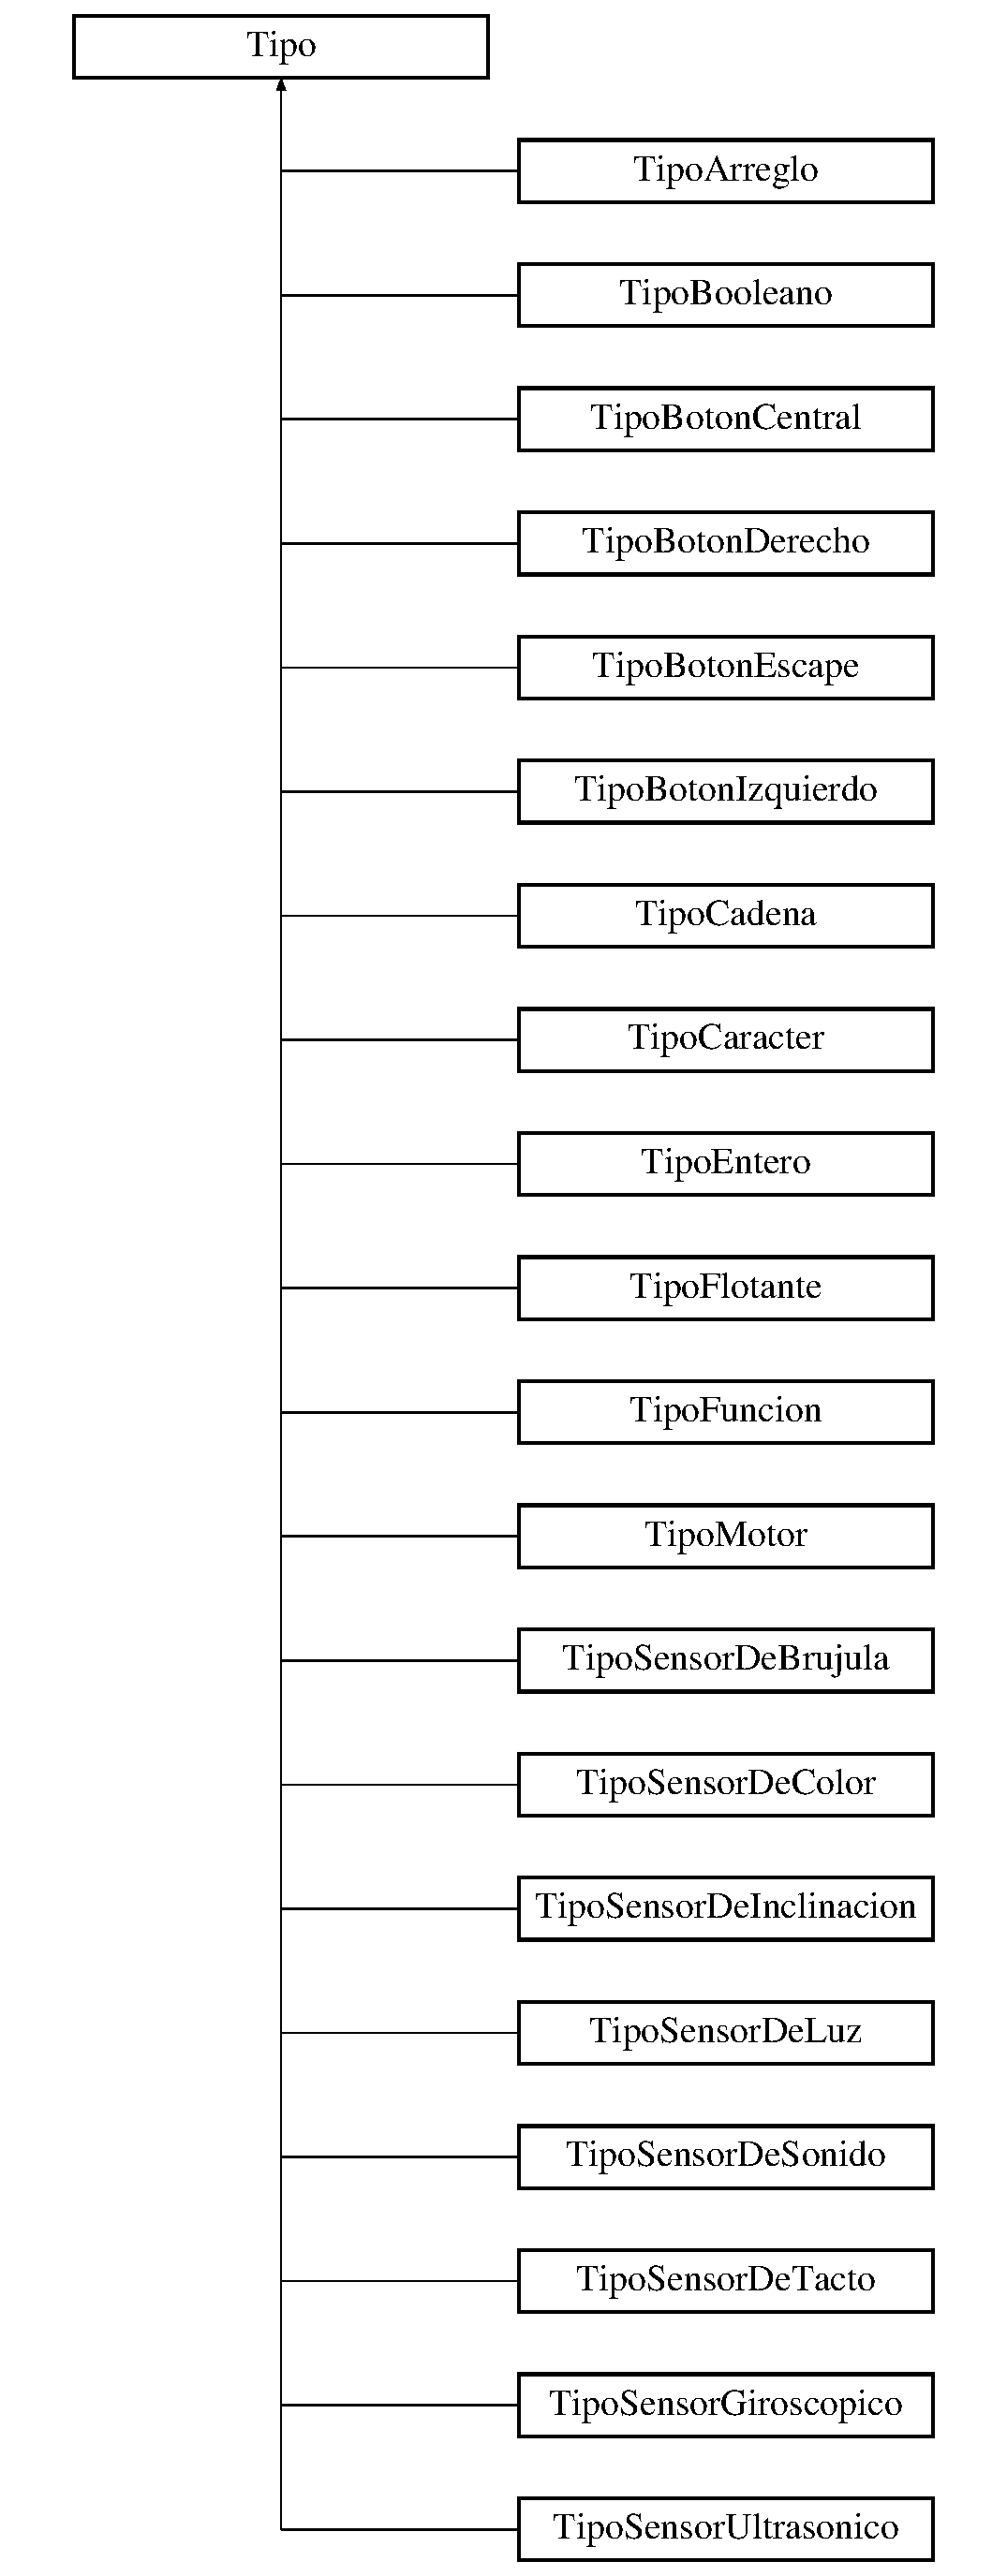
\includegraphics[height=12.000000cm]{class_tipo}
\end{center}
\end{figure}
\subsection*{Métodos públicos}
\begin{DoxyCompactItemize}
\item 
\hypertarget{class_tipo_afb62e2be23cab05bada0c0a94e0c1925}{{\bfseries Tipo} (Tipos tipo)}\label{class_tipo_afb62e2be23cab05bada0c0a94e0c1925}

\end{DoxyCompactItemize}
\subsection*{Atributos públicos}
\begin{DoxyCompactItemize}
\item 
\hypertarget{class_tipo_af707ea847ea3c1570a322cb8ad99ddf5}{Tipos {\bfseries tipo}}\label{class_tipo_af707ea847ea3c1570a322cb8ad99ddf5}

\end{DoxyCompactItemize}


La documentación para esta clase fue generada a partir de los siguientes ficheros\-:\begin{DoxyCompactItemize}
\item 
Programa/\-Tipos/Tipo.\-h\item 
Programa/\-Tipos/Tipo.\-cpp\end{DoxyCompactItemize}

\hypertarget{class_tipo_arreglo}{\section{Referencia de la Clase Tipo\-Arreglo}
\label{class_tipo_arreglo}\index{Tipo\-Arreglo@{Tipo\-Arreglo}}
}
Diagrama de herencias de Tipo\-Arreglo\begin{figure}[H]
\begin{center}
\leavevmode
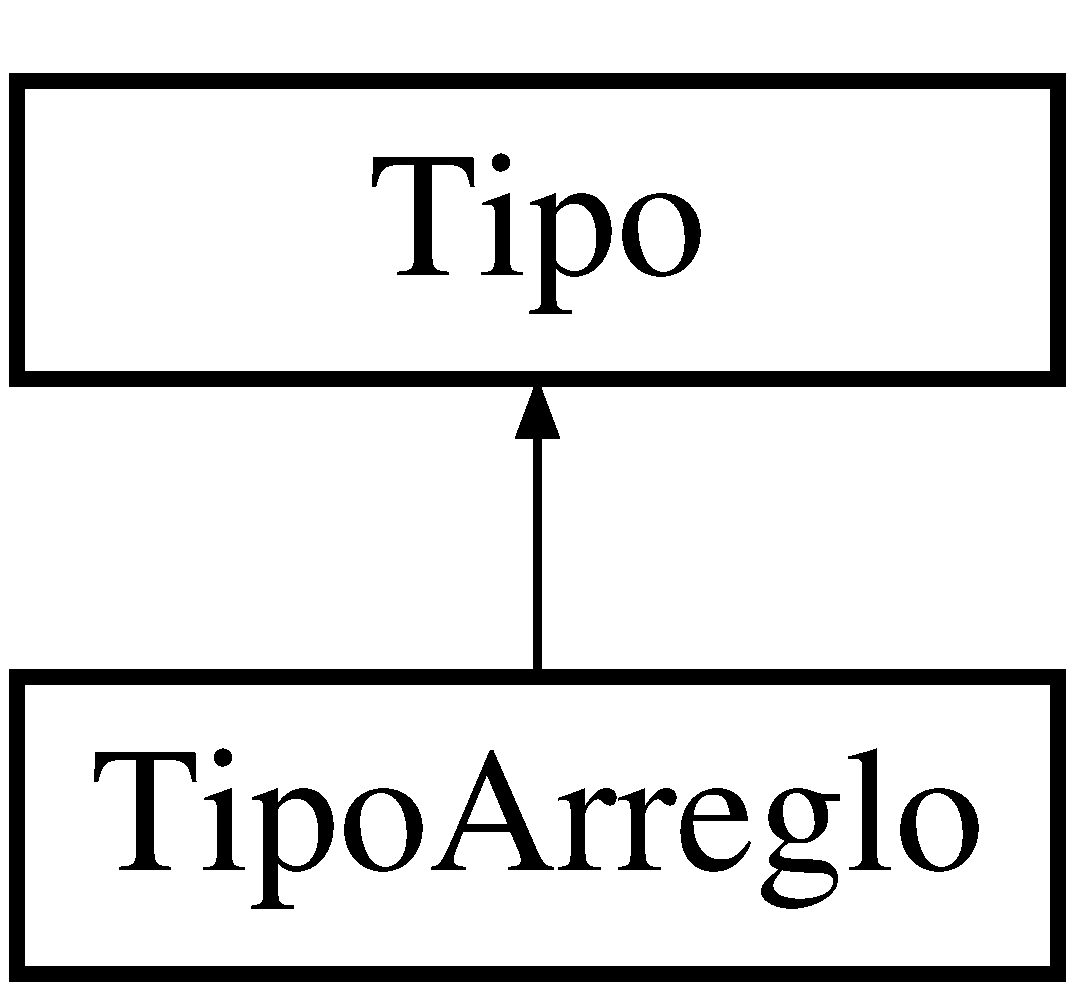
\includegraphics[height=2.000000cm]{class_tipo_arreglo}
\end{center}
\end{figure}
\subsection*{Otros miembros heredados}


La documentación para esta clase fue generada a partir de los siguientes ficheros\-:\begin{DoxyCompactItemize}
\item 
Programa/\-Tipos/Tipo\-Arreglo.\-h\item 
Programa/\-Tipos/Tipo\-Arreglo.\-cpp\end{DoxyCompactItemize}

\hypertarget{class_tipo_booleano}{\section{Referencia de la Clase Tipo\-Booleano}
\label{class_tipo_booleano}\index{Tipo\-Booleano@{Tipo\-Booleano}}
}
Diagrama de herencias de Tipo\-Booleano\begin{figure}[H]
\begin{center}
\leavevmode
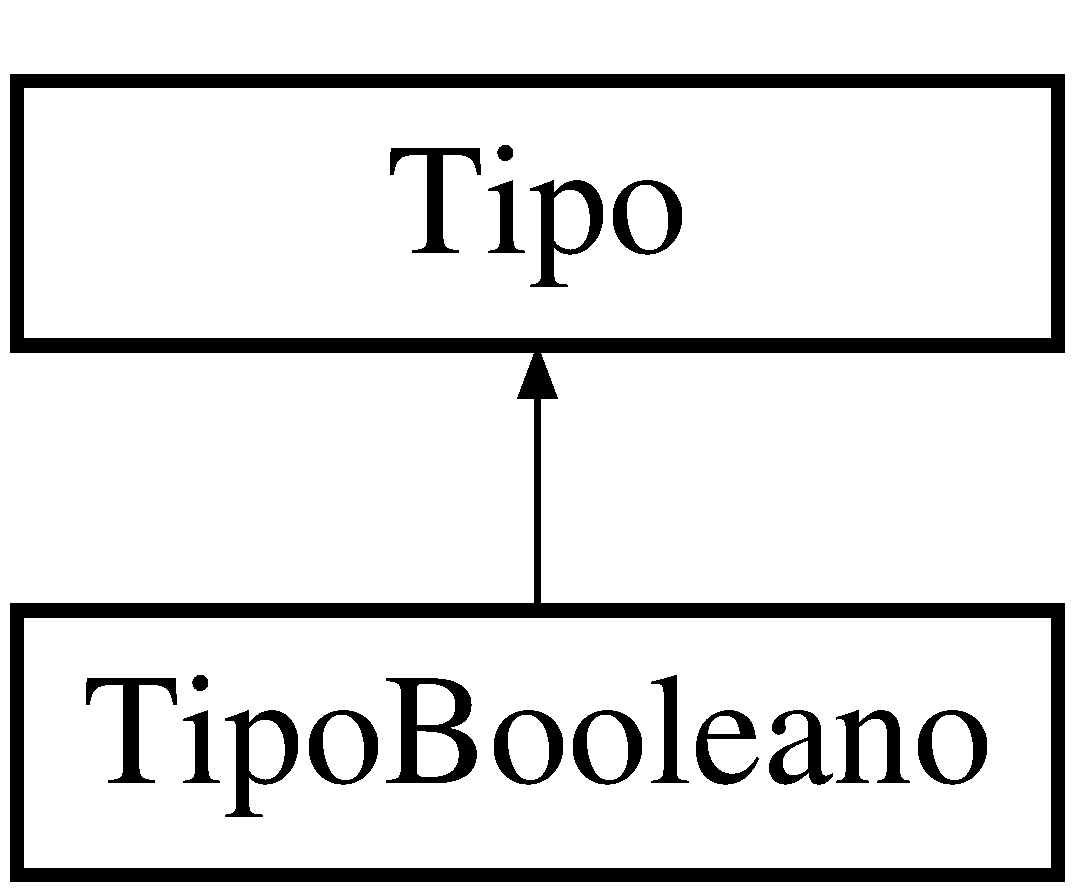
\includegraphics[height=2.000000cm]{class_tipo_booleano}
\end{center}
\end{figure}
\subsection*{Otros miembros heredados}


La documentación para esta clase fue generada a partir de los siguientes ficheros\-:\begin{DoxyCompactItemize}
\item 
Programa/\-Tipos/Tipo\-Booleano.\-h\item 
Programa/\-Tipos/Tipo\-Booleano.\-cpp\end{DoxyCompactItemize}

\hypertarget{class_tipo_boton_central}{\section{Referencia de la Clase Tipo\-Boton\-Central}
\label{class_tipo_boton_central}\index{Tipo\-Boton\-Central@{Tipo\-Boton\-Central}}
}
Diagrama de herencias de Tipo\-Boton\-Central\begin{figure}[H]
\begin{center}
\leavevmode
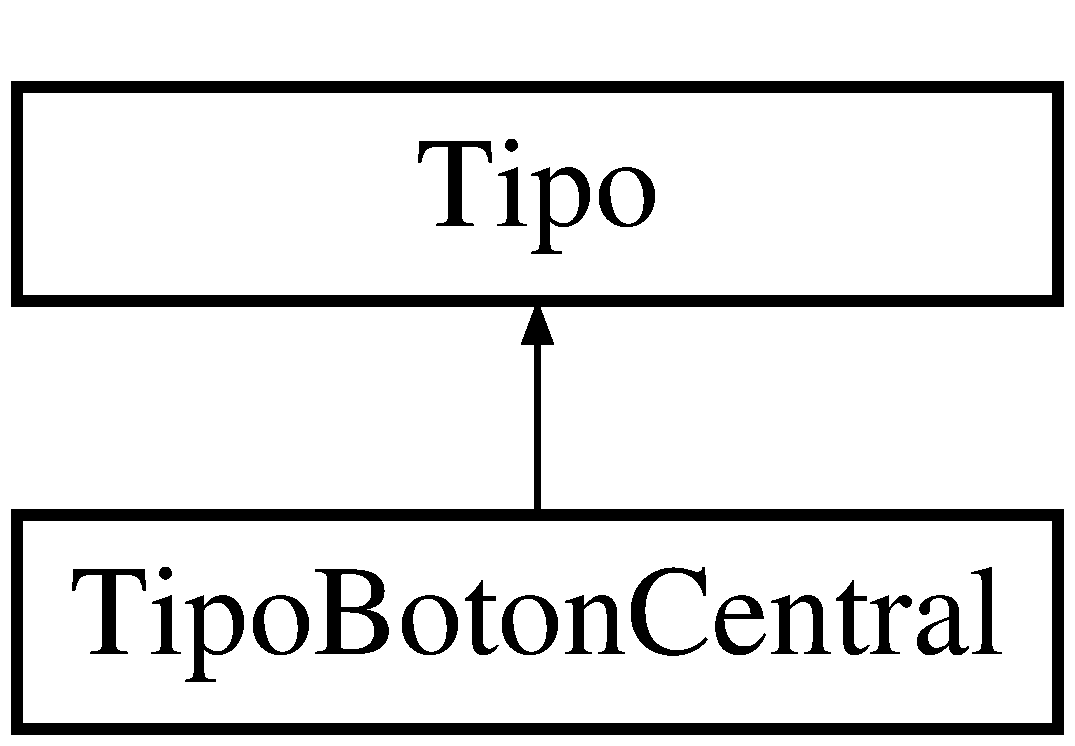
\includegraphics[height=2.000000cm]{class_tipo_boton_central}
\end{center}
\end{figure}
\subsection*{Otros miembros heredados}


La documentación para esta clase fue generada a partir de los siguientes ficheros\-:\begin{DoxyCompactItemize}
\item 
Programa/\-Tipos/Tipo\-Boton\-Central.\-h\item 
Programa/\-Tipos/Tipo\-Boton\-Central.\-cpp\end{DoxyCompactItemize}

\hypertarget{class_tipo_boton_derecho}{\section{Referencia de la Clase Tipo\-Boton\-Derecho}
\label{class_tipo_boton_derecho}\index{Tipo\-Boton\-Derecho@{Tipo\-Boton\-Derecho}}
}
Diagrama de herencias de Tipo\-Boton\-Derecho\begin{figure}[H]
\begin{center}
\leavevmode
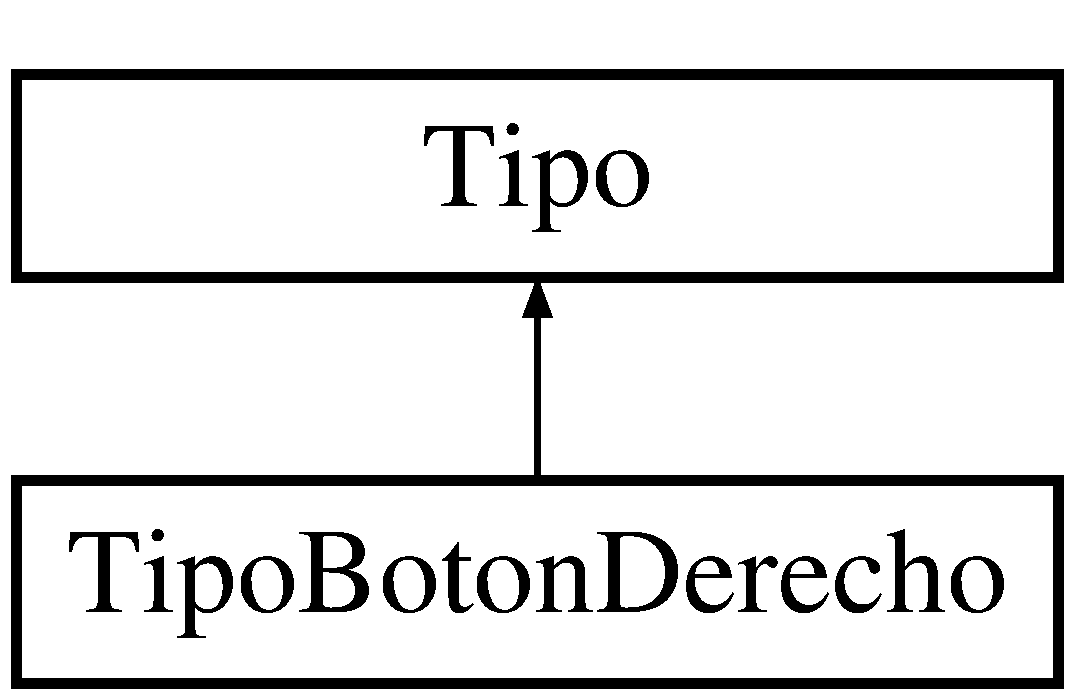
\includegraphics[height=2.000000cm]{class_tipo_boton_derecho}
\end{center}
\end{figure}
\subsection*{Otros miembros heredados}


La documentación para esta clase fue generada a partir de los siguientes ficheros\-:\begin{DoxyCompactItemize}
\item 
Programa/\-Tipos/Tipo\-Boton\-Derecho.\-h\item 
Programa/\-Tipos/Tipo\-Boton\-Derecho.\-cpp\end{DoxyCompactItemize}

\hypertarget{class_tipo_boton_escape}{\section{Referencia de la Clase Tipo\-Boton\-Escape}
\label{class_tipo_boton_escape}\index{Tipo\-Boton\-Escape@{Tipo\-Boton\-Escape}}
}
Diagrama de herencias de Tipo\-Boton\-Escape\begin{figure}[H]
\begin{center}
\leavevmode
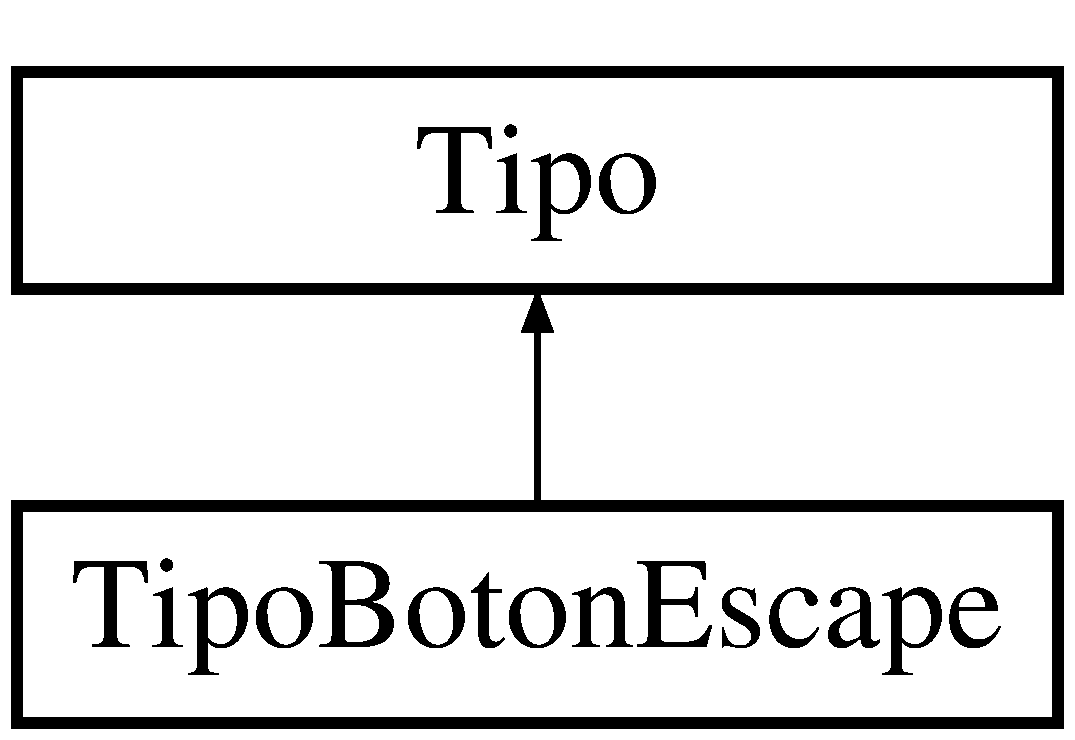
\includegraphics[height=2.000000cm]{class_tipo_boton_escape}
\end{center}
\end{figure}
\subsection*{Otros miembros heredados}


La documentación para esta clase fue generada a partir de los siguientes ficheros\-:\begin{DoxyCompactItemize}
\item 
Programa/\-Tipos/Tipo\-Boton\-Escape.\-h\item 
Programa/\-Tipos/Tipo\-Boton\-Escape.\-cpp\end{DoxyCompactItemize}

\hypertarget{class_tipo_boton_izquierdo}{\section{Referencia de la Clase Tipo\-Boton\-Izquierdo}
\label{class_tipo_boton_izquierdo}\index{Tipo\-Boton\-Izquierdo@{Tipo\-Boton\-Izquierdo}}
}
Diagrama de herencias de Tipo\-Boton\-Izquierdo\begin{figure}[H]
\begin{center}
\leavevmode
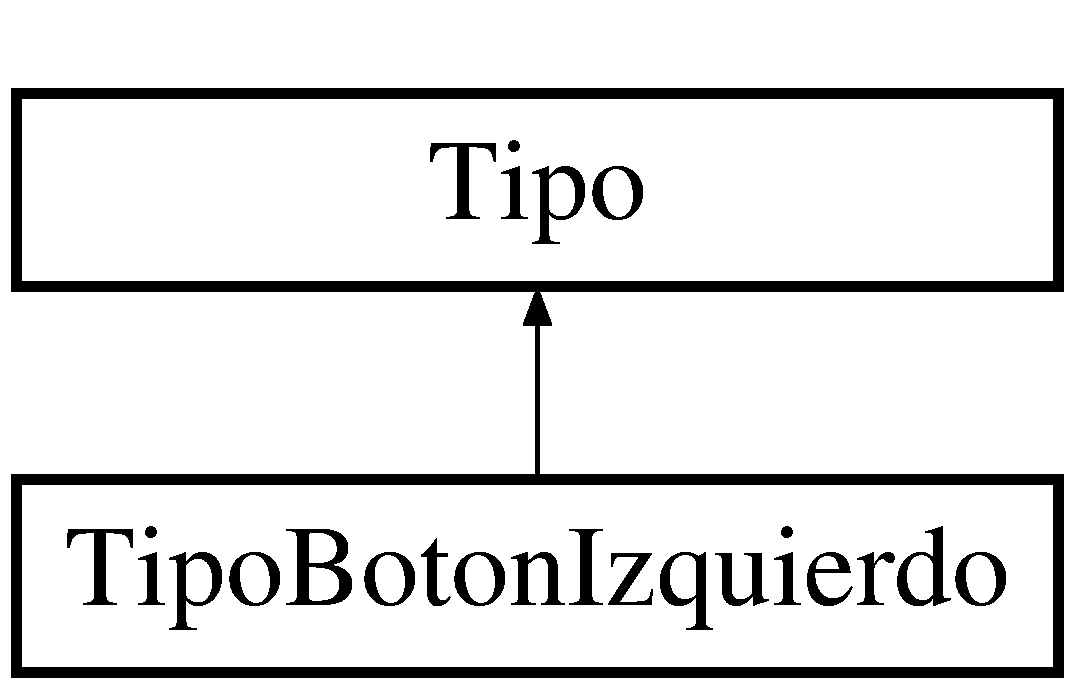
\includegraphics[height=2.000000cm]{class_tipo_boton_izquierdo}
\end{center}
\end{figure}
\subsection*{Otros miembros heredados}


La documentación para esta clase fue generada a partir de los siguientes ficheros\-:\begin{DoxyCompactItemize}
\item 
Programa/\-Tipos/Tipo\-Boton\-Izquierdo.\-h\item 
Programa/\-Tipos/Tipo\-Boton\-Izquierdo.\-cpp\end{DoxyCompactItemize}

\hypertarget{class_tipo_cadena}{\section{Referencia de la Clase Tipo\-Cadena}
\label{class_tipo_cadena}\index{Tipo\-Cadena@{Tipo\-Cadena}}
}
Diagrama de herencias de Tipo\-Cadena\begin{figure}[H]
\begin{center}
\leavevmode
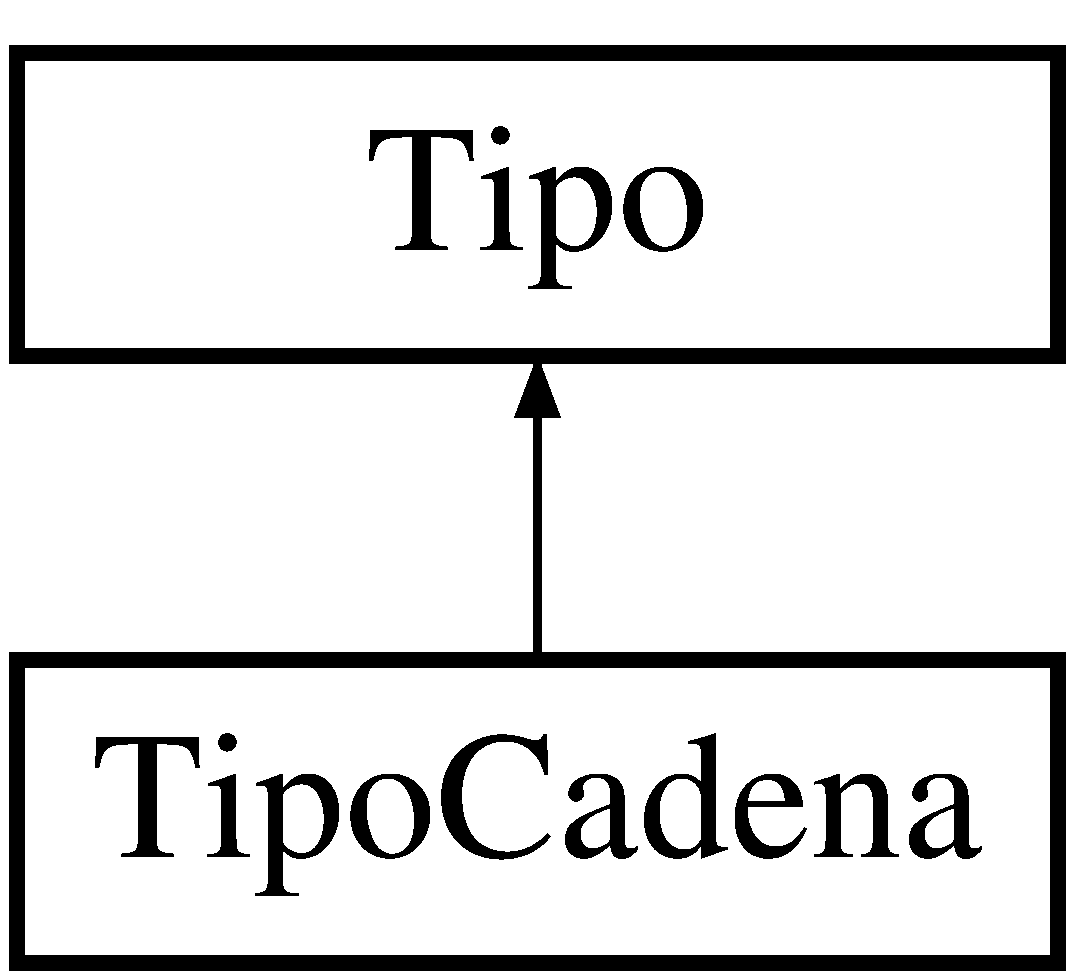
\includegraphics[height=2.000000cm]{class_tipo_cadena}
\end{center}
\end{figure}
\subsection*{Otros miembros heredados}


La documentación para esta clase fue generada a partir de los siguientes ficheros\-:\begin{DoxyCompactItemize}
\item 
Programa/\-Tipos/Tipo\-Cadena.\-h\item 
Programa/\-Tipos/Tipo\-Cadena.\-cpp\end{DoxyCompactItemize}

\hypertarget{class_tipo_caracter}{\section{Referencia de la Clase Tipo\-Caracter}
\label{class_tipo_caracter}\index{Tipo\-Caracter@{Tipo\-Caracter}}
}
Diagrama de herencias de Tipo\-Caracter\begin{figure}[H]
\begin{center}
\leavevmode
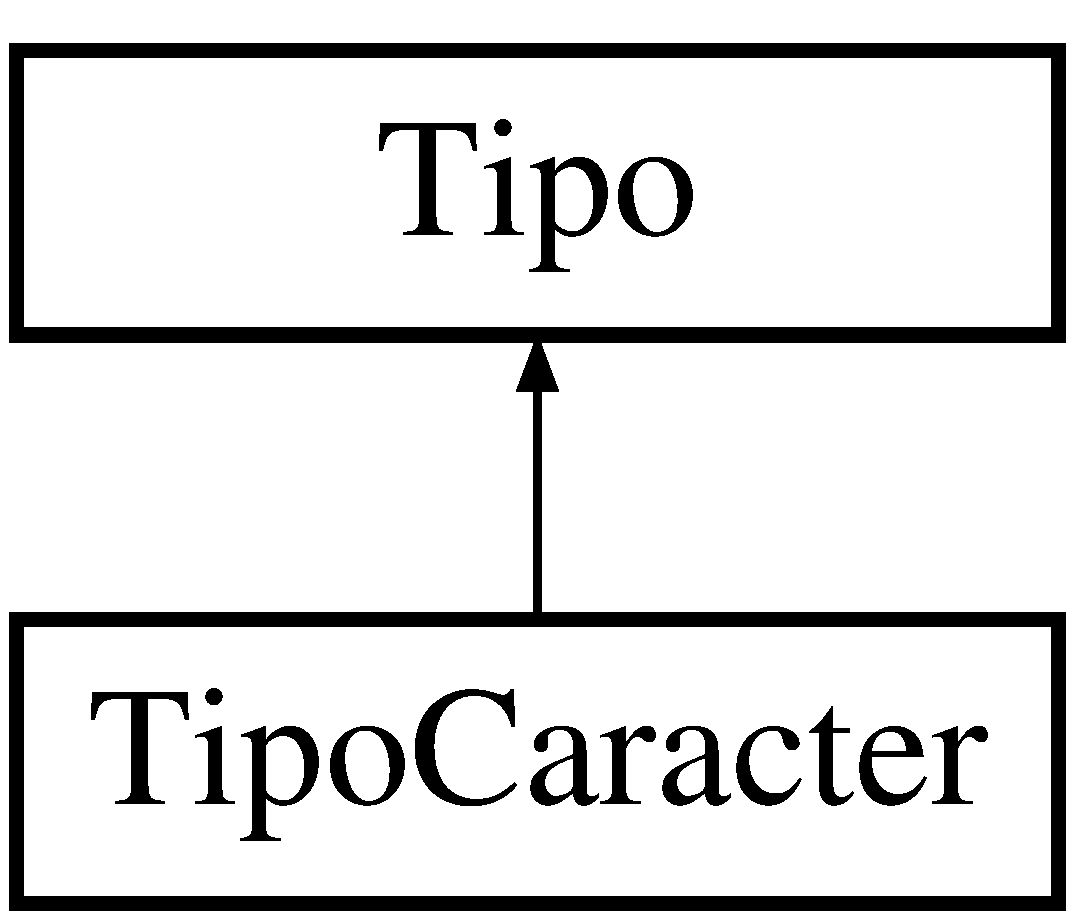
\includegraphics[height=2.000000cm]{class_tipo_caracter}
\end{center}
\end{figure}
\subsection*{Otros miembros heredados}


La documentación para esta clase fue generada a partir de los siguientes ficheros\-:\begin{DoxyCompactItemize}
\item 
Programa/\-Tipos/Tipo\-Caracter.\-h\item 
Programa/\-Tipos/Tipo\-Caracter.\-cpp\end{DoxyCompactItemize}

\hypertarget{class_tipo_entero}{\section{Referencia de la Clase Tipo\-Entero}
\label{class_tipo_entero}\index{Tipo\-Entero@{Tipo\-Entero}}
}
Diagrama de herencias de Tipo\-Entero\begin{figure}[H]
\begin{center}
\leavevmode
\includegraphics[height=2.000000cm]{class_tipo_entero}
\end{center}
\end{figure}
\subsection*{Otros miembros heredados}


La documentación para esta clase fue generada a partir de los siguientes ficheros\-:\begin{DoxyCompactItemize}
\item 
Programa/\-Tipos/Tipo\-Entero.\-h\item 
Programa/\-Tipos/Tipo\-Entero.\-cpp\end{DoxyCompactItemize}

\hypertarget{class_tipo_flotante}{\section{Referencia de la Clase Tipo\-Flotante}
\label{class_tipo_flotante}\index{Tipo\-Flotante@{Tipo\-Flotante}}
}
Diagrama de herencias de Tipo\-Flotante\begin{figure}[H]
\begin{center}
\leavevmode
\includegraphics[height=2.000000cm]{class_tipo_flotante}
\end{center}
\end{figure}
\subsection*{Otros miembros heredados}


La documentación para esta clase fue generada a partir de los siguientes ficheros\-:\begin{DoxyCompactItemize}
\item 
Programa/\-Tipos/Tipo\-Flotante.\-h\item 
Programa/\-Tipos/Tipo\-Flotante.\-cpp\end{DoxyCompactItemize}

\hypertarget{class_tipo_funcion}{\section{Referencia de la Clase Tipo\-Funcion}
\label{class_tipo_funcion}\index{Tipo\-Funcion@{Tipo\-Funcion}}
}
Diagrama de herencias de Tipo\-Funcion\begin{figure}[H]
\begin{center}
\leavevmode
\includegraphics[height=2.000000cm]{class_tipo_funcion}
\end{center}
\end{figure}
\subsection*{Otros miembros heredados}


La documentación para esta clase fue generada a partir de los siguientes ficheros\-:\begin{DoxyCompactItemize}
\item 
Programa/\-Tipos/Tipo\-Funcion.\-h\item 
Programa/\-Tipos/Tipo\-Funcion.\-cpp\end{DoxyCompactItemize}

\hypertarget{class_tipo_motor}{\section{Referencia de la Clase Tipo\-Motor}
\label{class_tipo_motor}\index{Tipo\-Motor@{Tipo\-Motor}}
}
Diagrama de herencias de Tipo\-Motor\begin{figure}[H]
\begin{center}
\leavevmode
\includegraphics[height=2.000000cm]{class_tipo_motor}
\end{center}
\end{figure}
\subsection*{Otros miembros heredados}


La documentación para esta clase fue generada a partir de los siguientes ficheros\-:\begin{DoxyCompactItemize}
\item 
Programa/\-Tipos/Tipo\-Motor.\-h\item 
Programa/\-Tipos/Tipo\-Motor.\-cpp\end{DoxyCompactItemize}

\hypertarget{class_tipo_sensor_de_brujula}{\section{Referencia de la Clase Tipo\-Sensor\-De\-Brujula}
\label{class_tipo_sensor_de_brujula}\index{Tipo\-Sensor\-De\-Brujula@{Tipo\-Sensor\-De\-Brujula}}
}
Diagrama de herencias de Tipo\-Sensor\-De\-Brujula\begin{figure}[H]
\begin{center}
\leavevmode
\includegraphics[height=2.000000cm]{class_tipo_sensor_de_brujula}
\end{center}
\end{figure}
\subsection*{Otros miembros heredados}


La documentación para esta clase fue generada a partir de los siguientes ficheros\-:\begin{DoxyCompactItemize}
\item 
Programa/\-Tipos/Tipo\-Sensor\-De\-Brujula.\-h\item 
Programa/\-Tipos/Tipo\-Sensor\-De\-Brujula.\-cpp\end{DoxyCompactItemize}

\hypertarget{class_tipo_sensor_de_color}{\section{Referencia de la Clase Tipo\-Sensor\-De\-Color}
\label{class_tipo_sensor_de_color}\index{Tipo\-Sensor\-De\-Color@{Tipo\-Sensor\-De\-Color}}
}
Diagrama de herencias de Tipo\-Sensor\-De\-Color\begin{figure}[H]
\begin{center}
\leavevmode
\includegraphics[height=2.000000cm]{class_tipo_sensor_de_color}
\end{center}
\end{figure}
\subsection*{Otros miembros heredados}


La documentación para esta clase fue generada a partir de los siguientes ficheros\-:\begin{DoxyCompactItemize}
\item 
Programa/\-Tipos/Tipo\-Sensor\-De\-Color.\-h\item 
Programa/\-Tipos/Tipo\-Sensor\-De\-Color.\-cpp\end{DoxyCompactItemize}

\hypertarget{class_tipo_sensor_de_inclinacion}{\section{Referencia de la Clase Tipo\-Sensor\-De\-Inclinacion}
\label{class_tipo_sensor_de_inclinacion}\index{Tipo\-Sensor\-De\-Inclinacion@{Tipo\-Sensor\-De\-Inclinacion}}
}
Diagrama de herencias de Tipo\-Sensor\-De\-Inclinacion\begin{figure}[H]
\begin{center}
\leavevmode
\includegraphics[height=2.000000cm]{class_tipo_sensor_de_inclinacion}
\end{center}
\end{figure}
\subsection*{Otros miembros heredados}


La documentación para esta clase fue generada a partir de los siguientes ficheros\-:\begin{DoxyCompactItemize}
\item 
Programa/\-Tipos/Tipo\-Sensor\-De\-Inclinacion.\-h\item 
Programa/\-Tipos/Tipo\-Sensor\-De\-Inclinacion.\-cpp\end{DoxyCompactItemize}

\hypertarget{class_tipo_sensor_de_luz}{\section{Referencia de la Clase Tipo\-Sensor\-De\-Luz}
\label{class_tipo_sensor_de_luz}\index{Tipo\-Sensor\-De\-Luz@{Tipo\-Sensor\-De\-Luz}}
}
Diagrama de herencias de Tipo\-Sensor\-De\-Luz\begin{figure}[H]
\begin{center}
\leavevmode
\includegraphics[height=2.000000cm]{class_tipo_sensor_de_luz}
\end{center}
\end{figure}
\subsection*{Otros miembros heredados}


La documentación para esta clase fue generada a partir de los siguientes ficheros\-:\begin{DoxyCompactItemize}
\item 
Programa/\-Tipos/Tipo\-Sensor\-De\-Luz.\-h\item 
Programa/\-Tipos/Tipo\-Sensor\-De\-Luz.\-cpp\end{DoxyCompactItemize}

\hypertarget{class_tipo_sensor_de_sonido}{\section{Referencia de la Clase Tipo\-Sensor\-De\-Sonido}
\label{class_tipo_sensor_de_sonido}\index{Tipo\-Sensor\-De\-Sonido@{Tipo\-Sensor\-De\-Sonido}}
}
Diagrama de herencias de Tipo\-Sensor\-De\-Sonido\begin{figure}[H]
\begin{center}
\leavevmode
\includegraphics[height=2.000000cm]{class_tipo_sensor_de_sonido}
\end{center}
\end{figure}
\subsection*{Otros miembros heredados}


La documentación para esta clase fue generada a partir de los siguientes ficheros\-:\begin{DoxyCompactItemize}
\item 
Programa/\-Tipos/Tipo\-Sensor\-De\-Sonido.\-h\item 
Programa/\-Tipos/Tipo\-Sensor\-De\-Sonido.\-cpp\end{DoxyCompactItemize}

\hypertarget{class_tipo_sensor_de_tacto}{\section{Referencia de la Clase Tipo\-Sensor\-De\-Tacto}
\label{class_tipo_sensor_de_tacto}\index{Tipo\-Sensor\-De\-Tacto@{Tipo\-Sensor\-De\-Tacto}}
}
Diagrama de herencias de Tipo\-Sensor\-De\-Tacto\begin{figure}[H]
\begin{center}
\leavevmode
\includegraphics[height=2.000000cm]{class_tipo_sensor_de_tacto}
\end{center}
\end{figure}
\subsection*{Otros miembros heredados}


La documentación para esta clase fue generada a partir de los siguientes ficheros\-:\begin{DoxyCompactItemize}
\item 
Programa/\-Tipos/Tipo\-Sensor\-De\-Tacto.\-h\item 
Programa/\-Tipos/Tipo\-Sensor\-De\-Tacto.\-cpp\end{DoxyCompactItemize}

\hypertarget{class_tipo_sensor_giroscopico}{\section{Referencia de la Clase Tipo\-Sensor\-Giroscopico}
\label{class_tipo_sensor_giroscopico}\index{Tipo\-Sensor\-Giroscopico@{Tipo\-Sensor\-Giroscopico}}
}
Diagrama de herencias de Tipo\-Sensor\-Giroscopico\begin{figure}[H]
\begin{center}
\leavevmode
\includegraphics[height=2.000000cm]{class_tipo_sensor_giroscopico}
\end{center}
\end{figure}
\subsection*{Otros miembros heredados}


La documentación para esta clase fue generada a partir de los siguientes ficheros\-:\begin{DoxyCompactItemize}
\item 
Programa/\-Tipos/Tipo\-Sensor\-Giroscopico.\-h\item 
Programa/\-Tipos/Tipo\-Sensor\-Giroscopico.\-cpp\end{DoxyCompactItemize}

\hypertarget{class_tipo_sensor_ultrasonico}{\section{Referencia de la Clase Tipo\-Sensor\-Ultrasonico}
\label{class_tipo_sensor_ultrasonico}\index{Tipo\-Sensor\-Ultrasonico@{Tipo\-Sensor\-Ultrasonico}}
}
Diagrama de herencias de Tipo\-Sensor\-Ultrasonico\begin{figure}[H]
\begin{center}
\leavevmode
\includegraphics[height=2.000000cm]{class_tipo_sensor_ultrasonico}
\end{center}
\end{figure}
\subsection*{Otros miembros heredados}


La documentación para esta clase fue generada a partir de los siguientes ficheros\-:\begin{DoxyCompactItemize}
\item 
Programa/\-Tipos/Tipo\-Sensor\-Ultrasonico.\-h\item 
Programa/\-Tipos/Tipo\-Sensor\-Ultrasonico.\-cpp\end{DoxyCompactItemize}

\hypertarget{class_ti_xml_attribute}{\section{Referencia de la Clase Ti\-Xml\-Attribute}
\label{class_ti_xml_attribute}\index{Ti\-Xml\-Attribute@{Ti\-Xml\-Attribute}}
}


{\ttfamily \#include $<$tinyxml.\-h$>$}

Diagrama de herencias de Ti\-Xml\-Attribute\begin{figure}[H]
\begin{center}
\leavevmode
\includegraphics[height=2.000000cm]{class_ti_xml_attribute}
\end{center}
\end{figure}
\subsection*{Métodos públicos}
\begin{DoxyCompactItemize}
\item 
\hypertarget{class_ti_xml_attribute_a9cfa3c8179873fd485d83003b114f8e1}{\hyperlink{class_ti_xml_attribute_a9cfa3c8179873fd485d83003b114f8e1}{Ti\-Xml\-Attribute} ()}\label{class_ti_xml_attribute_a9cfa3c8179873fd485d83003b114f8e1}

\begin{DoxyCompactList}\small\item\em Construct an empty attribute. \end{DoxyCompactList}\item 
\hypertarget{class_ti_xml_attribute_a759d0b76fb8fcf765ecab243bc14f05e}{\hyperlink{class_ti_xml_attribute_a759d0b76fb8fcf765ecab243bc14f05e}{Ti\-Xml\-Attribute} (const char $\ast$\-\_\-name, const char $\ast$\-\_\-value)}\label{class_ti_xml_attribute_a759d0b76fb8fcf765ecab243bc14f05e}

\begin{DoxyCompactList}\small\item\em Construct an attribute with a name and value. \end{DoxyCompactList}\item 
\hypertarget{class_ti_xml_attribute_a298a57287d305904ba6bd96ae6f78d3d}{const char $\ast$ \hyperlink{class_ti_xml_attribute_a298a57287d305904ba6bd96ae6f78d3d}{Name} () const }\label{class_ti_xml_attribute_a298a57287d305904ba6bd96ae6f78d3d}

\begin{DoxyCompactList}\small\item\em Return the name of this attribute. \end{DoxyCompactList}\item 
\hypertarget{class_ti_xml_attribute_a0f874490eac8ca00ee0070765d0e97e3}{const char $\ast$ \hyperlink{class_ti_xml_attribute_a0f874490eac8ca00ee0070765d0e97e3}{Value} () const }\label{class_ti_xml_attribute_a0f874490eac8ca00ee0070765d0e97e3}

\begin{DoxyCompactList}\small\item\em Return the value of this attribute. \end{DoxyCompactList}\item 
\hypertarget{class_ti_xml_attribute_aa1a20ad59dc7e89a0ab265396360d50f}{int \hyperlink{class_ti_xml_attribute_aa1a20ad59dc7e89a0ab265396360d50f}{Int\-Value} () const }\label{class_ti_xml_attribute_aa1a20ad59dc7e89a0ab265396360d50f}

\begin{DoxyCompactList}\small\item\em Return the value of this attribute, converted to an integer. \end{DoxyCompactList}\item 
\hypertarget{class_ti_xml_attribute_a2880ddef53fc7522c99535273954d230}{double \hyperlink{class_ti_xml_attribute_a2880ddef53fc7522c99535273954d230}{Double\-Value} () const }\label{class_ti_xml_attribute_a2880ddef53fc7522c99535273954d230}

\begin{DoxyCompactList}\small\item\em Return the value of this attribute, converted to a double. \end{DoxyCompactList}\item 
\hypertarget{class_ti_xml_attribute_a64cee17bceb8232eb0736d26dd082d79}{const T\-I\-X\-M\-L\-\_\-\-S\-T\-R\-I\-N\-G \& {\bfseries Name\-T\-Str} () const }\label{class_ti_xml_attribute_a64cee17bceb8232eb0736d26dd082d79}

\item 
int \hyperlink{class_ti_xml_attribute_ad6c93088ee21af41a107931223339344}{Query\-Int\-Value} (int $\ast$\-\_\-value) const 
\item 
\hypertarget{class_ti_xml_attribute_ac87b2a8489906a5d7aa2875f20be3513}{int \hyperlink{class_ti_xml_attribute_ac87b2a8489906a5d7aa2875f20be3513}{Query\-Double\-Value} (double $\ast$\-\_\-value) const }\label{class_ti_xml_attribute_ac87b2a8489906a5d7aa2875f20be3513}

\begin{DoxyCompactList}\small\item\em Query\-Double\-Value examines the value string. See \hyperlink{class_ti_xml_attribute_ad6c93088ee21af41a107931223339344}{Query\-Int\-Value()}. \end{DoxyCompactList}\item 
\hypertarget{class_ti_xml_attribute_ab7fa3d21ff8d7c5764cf9af15b667a99}{void \hyperlink{class_ti_xml_attribute_ab7fa3d21ff8d7c5764cf9af15b667a99}{Set\-Name} (const char $\ast$\-\_\-name)}\label{class_ti_xml_attribute_ab7fa3d21ff8d7c5764cf9af15b667a99}

\begin{DoxyCompactList}\small\item\em Set the name of this attribute. \end{DoxyCompactList}\item 
\hypertarget{class_ti_xml_attribute_a2dae44178f668b3cb48101be4f2236a0}{void \hyperlink{class_ti_xml_attribute_a2dae44178f668b3cb48101be4f2236a0}{Set\-Value} (const char $\ast$\-\_\-value)}\label{class_ti_xml_attribute_a2dae44178f668b3cb48101be4f2236a0}

\begin{DoxyCompactList}\small\item\em Set the value. \end{DoxyCompactList}\item 
\hypertarget{class_ti_xml_attribute_a7e065df640116a62ea4f4b7da5449cc8}{void \hyperlink{class_ti_xml_attribute_a7e065df640116a62ea4f4b7da5449cc8}{Set\-Int\-Value} (int \-\_\-value)}\label{class_ti_xml_attribute_a7e065df640116a62ea4f4b7da5449cc8}

\begin{DoxyCompactList}\small\item\em Set the value from an integer. \end{DoxyCompactList}\item 
\hypertarget{class_ti_xml_attribute_a0316da31373496c4368ad549bf711394}{void \hyperlink{class_ti_xml_attribute_a0316da31373496c4368ad549bf711394}{Set\-Double\-Value} (double \-\_\-value)}\label{class_ti_xml_attribute_a0316da31373496c4368ad549bf711394}

\begin{DoxyCompactList}\small\item\em Set the value from a double. \end{DoxyCompactList}\item 
\hypertarget{class_ti_xml_attribute_a776478980776a024f7c2846eec640f65}{const \hyperlink{class_ti_xml_attribute}{Ti\-Xml\-Attribute} $\ast$ \hyperlink{class_ti_xml_attribute_a776478980776a024f7c2846eec640f65}{Next} () const }\label{class_ti_xml_attribute_a776478980776a024f7c2846eec640f65}

\begin{DoxyCompactList}\small\item\em Get the next sibling attribute in the D\-O\-M. Returns null at end. \end{DoxyCompactList}\item 
\hypertarget{class_ti_xml_attribute_a138320aa7793b148ba7e5bd0a0ea4db6}{\hyperlink{class_ti_xml_attribute}{Ti\-Xml\-Attribute} $\ast$ {\bfseries Next} ()}\label{class_ti_xml_attribute_a138320aa7793b148ba7e5bd0a0ea4db6}

\item 
\hypertarget{class_ti_xml_attribute_a54a5f8730c7b02b9a41b74e12e27fe86}{const \hyperlink{class_ti_xml_attribute}{Ti\-Xml\-Attribute} $\ast$ \hyperlink{class_ti_xml_attribute_a54a5f8730c7b02b9a41b74e12e27fe86}{Previous} () const }\label{class_ti_xml_attribute_a54a5f8730c7b02b9a41b74e12e27fe86}

\begin{DoxyCompactList}\small\item\em Get the previous sibling attribute in the D\-O\-M. Returns null at beginning. \end{DoxyCompactList}\item 
\hypertarget{class_ti_xml_attribute_ae4dabc932cba945ed1e92fec5f121193}{\hyperlink{class_ti_xml_attribute}{Ti\-Xml\-Attribute} $\ast$ {\bfseries Previous} ()}\label{class_ti_xml_attribute_ae4dabc932cba945ed1e92fec5f121193}

\item 
\hypertarget{class_ti_xml_attribute_ae48c2a65b520d453914ce4e845d607cf}{bool {\bfseries operator==} (const \hyperlink{class_ti_xml_attribute}{Ti\-Xml\-Attribute} \&rhs) const }\label{class_ti_xml_attribute_ae48c2a65b520d453914ce4e845d607cf}

\item 
\hypertarget{class_ti_xml_attribute_adb8b6f2cad5948e73e383182e7ce10de}{bool {\bfseries operator$<$} (const \hyperlink{class_ti_xml_attribute}{Ti\-Xml\-Attribute} \&rhs) const }\label{class_ti_xml_attribute_adb8b6f2cad5948e73e383182e7ce10de}

\item 
\hypertarget{class_ti_xml_attribute_a867562769ef9778c1690cd373246b05b}{bool {\bfseries operator$>$} (const \hyperlink{class_ti_xml_attribute}{Ti\-Xml\-Attribute} \&rhs) const }\label{class_ti_xml_attribute_a867562769ef9778c1690cd373246b05b}

\item 
\hypertarget{class_ti_xml_attribute_ad62774421b814894b995af3b5d231dda}{virtual const char $\ast$ {\bfseries Parse} (const char $\ast$p, \hyperlink{class_ti_xml_parsing_data}{Ti\-Xml\-Parsing\-Data} $\ast$data, Ti\-Xml\-Encoding encoding)}\label{class_ti_xml_attribute_ad62774421b814894b995af3b5d231dda}

\item 
virtual void \hyperlink{class_ti_xml_attribute_acc04956c1d5c4c31fe74f7a7528d109a}{Print} (F\-I\-L\-E $\ast$cfile, int depth) const 
\item 
\hypertarget{class_ti_xml_attribute_a19e6b6862a80b188571c47947e88d030}{void {\bfseries Print} (F\-I\-L\-E $\ast$cfile, int depth, T\-I\-X\-M\-L\-\_\-\-S\-T\-R\-I\-N\-G $\ast$str) const }\label{class_ti_xml_attribute_a19e6b6862a80b188571c47947e88d030}

\item 
\hypertarget{class_ti_xml_attribute_ac12a94d4548302afb12f488ba101f7d1}{void {\bfseries Set\-Document} (\hyperlink{class_ti_xml_document}{Ti\-Xml\-Document} $\ast$doc)}\label{class_ti_xml_attribute_ac12a94d4548302afb12f488ba101f7d1}

\end{DoxyCompactItemize}
\subsection*{Amigas}
\begin{DoxyCompactItemize}
\item 
\hypertarget{class_ti_xml_attribute_a35a7b7f89f708527677d5078d41ce0bf}{class {\bfseries Ti\-Xml\-Attribute\-Set}}\label{class_ti_xml_attribute_a35a7b7f89f708527677d5078d41ce0bf}

\end{DoxyCompactItemize}
\subsection*{Otros miembros heredados}


\subsection{Descripción detallada}
An attribute is a name-\/value pair. Elements have an arbitrary number of attributes, each with a unique name.

\begin{DoxyNote}{Nota}
The attributes are not Ti\-Xml\-Nodes, since they are not part of the tiny\-X\-M\-L document object model. There are other suggested ways to look at this problem. 
\end{DoxyNote}


\subsection{Documentación de las funciones miembro}
\hypertarget{class_ti_xml_attribute_acc04956c1d5c4c31fe74f7a7528d109a}{\index{Ti\-Xml\-Attribute@{Ti\-Xml\-Attribute}!Print@{Print}}
\index{Print@{Print}!TiXmlAttribute@{Ti\-Xml\-Attribute}}
\subsubsection[{Print}]{\setlength{\rightskip}{0pt plus 5cm}virtual void Ti\-Xml\-Attribute\-::\-Print (
\begin{DoxyParamCaption}
\item[{F\-I\-L\-E $\ast$}]{cfile, }
\item[{int}]{depth}
\end{DoxyParamCaption}
) const\hspace{0.3cm}{\ttfamily [inline]}, {\ttfamily [virtual]}}}\label{class_ti_xml_attribute_acc04956c1d5c4c31fe74f7a7528d109a}
All Tiny\-Xml classes can print themselves to a filestream or the string class (\hyperlink{class_ti_xml_string}{Ti\-Xml\-String} in non-\/\-S\-T\-L mode, std\-::string in S\-T\-L mode.) Either or both cfile and str can be null.

This is a formatted print, and will insert tabs and newlines.

(For an unformatted stream, use the $<$$<$ operator.) 

Implementa \hyperlink{class_ti_xml_base_a0de56b3f2ef14c65091a3b916437b512}{Ti\-Xml\-Base}.

\hypertarget{class_ti_xml_attribute_ad6c93088ee21af41a107931223339344}{\index{Ti\-Xml\-Attribute@{Ti\-Xml\-Attribute}!Query\-Int\-Value@{Query\-Int\-Value}}
\index{Query\-Int\-Value@{Query\-Int\-Value}!TiXmlAttribute@{Ti\-Xml\-Attribute}}
\subsubsection[{Query\-Int\-Value}]{\setlength{\rightskip}{0pt plus 5cm}int Ti\-Xml\-Attribute\-::\-Query\-Int\-Value (
\begin{DoxyParamCaption}
\item[{int $\ast$}]{\-\_\-value}
\end{DoxyParamCaption}
) const}}\label{class_ti_xml_attribute_ad6c93088ee21af41a107931223339344}
Query\-Int\-Value examines the value string. It is an alternative to the \hyperlink{class_ti_xml_attribute_aa1a20ad59dc7e89a0ab265396360d50f}{Int\-Value()} method with richer error checking. If the value is an integer, it is stored in 'value' and the call returns T\-I\-X\-M\-L\-\_\-\-S\-U\-C\-C\-E\-S\-S. If it is not an integer, it returns T\-I\-X\-M\-L\-\_\-\-W\-R\-O\-N\-G\-\_\-\-T\-Y\-P\-E.

A specialized but useful call. Note that for success it returns 0, which is the opposite of almost all other Tiny\-Xml calls. 

La documentación para esta clase fue generada a partir de los siguientes ficheros\-:\begin{DoxyCompactItemize}
\item 
Tiny\-X\-M\-L/tinyxml.\-h\item 
Tiny\-X\-M\-L/tinyxml.\-cpp\item 
Tiny\-X\-M\-L/tinyxmlparser.\-cpp\end{DoxyCompactItemize}

\hypertarget{class_ti_xml_attribute_set}{\section{Referencia de la Clase Ti\-Xml\-Attribute\-Set}
\label{class_ti_xml_attribute_set}\index{Ti\-Xml\-Attribute\-Set@{Ti\-Xml\-Attribute\-Set}}
}
\subsection*{Métodos públicos}
\begin{DoxyCompactItemize}
\item 
\hypertarget{class_ti_xml_attribute_set_a745e50ddaae3bee93e4589321e0b9c1a}{void {\bfseries Add} (\hyperlink{class_ti_xml_attribute}{Ti\-Xml\-Attribute} $\ast$attribute)}\label{class_ti_xml_attribute_set_a745e50ddaae3bee93e4589321e0b9c1a}

\item 
\hypertarget{class_ti_xml_attribute_set_a924a73d071f2573f9060f0be57879c57}{void {\bfseries Remove} (\hyperlink{class_ti_xml_attribute}{Ti\-Xml\-Attribute} $\ast$attribute)}\label{class_ti_xml_attribute_set_a924a73d071f2573f9060f0be57879c57}

\item 
\hypertarget{class_ti_xml_attribute_set_ae0636e88cedd4b09d61c451860f68598}{const \hyperlink{class_ti_xml_attribute}{Ti\-Xml\-Attribute} $\ast$ {\bfseries First} () const }\label{class_ti_xml_attribute_set_ae0636e88cedd4b09d61c451860f68598}

\item 
\hypertarget{class_ti_xml_attribute_set_a99703bb08ca2aece2d7ef835de339ba0}{\hyperlink{class_ti_xml_attribute}{Ti\-Xml\-Attribute} $\ast$ {\bfseries First} ()}\label{class_ti_xml_attribute_set_a99703bb08ca2aece2d7ef835de339ba0}

\item 
\hypertarget{class_ti_xml_attribute_set_a7b3f3ccf39a97bc25539d3fcc540296a}{const \hyperlink{class_ti_xml_attribute}{Ti\-Xml\-Attribute} $\ast$ {\bfseries Last} () const }\label{class_ti_xml_attribute_set_a7b3f3ccf39a97bc25539d3fcc540296a}

\item 
\hypertarget{class_ti_xml_attribute_set_ab4c4edfb2d74f6ea31aae096743bd6e0}{\hyperlink{class_ti_xml_attribute}{Ti\-Xml\-Attribute} $\ast$ {\bfseries Last} ()}\label{class_ti_xml_attribute_set_ab4c4edfb2d74f6ea31aae096743bd6e0}

\item 
\hypertarget{class_ti_xml_attribute_set_af3675cc2bfd0aea153cda1cfcdd1f77e}{\hyperlink{class_ti_xml_attribute}{Ti\-Xml\-Attribute} $\ast$ {\bfseries Find} (const char $\ast$\-\_\-name) const }\label{class_ti_xml_attribute_set_af3675cc2bfd0aea153cda1cfcdd1f77e}

\item 
\hypertarget{class_ti_xml_attribute_set_a5e28f5d32f048fba85d04dc317495bdc}{\hyperlink{class_ti_xml_attribute}{Ti\-Xml\-Attribute} $\ast$ {\bfseries Find\-Or\-Create} (const char $\ast$\-\_\-name)}\label{class_ti_xml_attribute_set_a5e28f5d32f048fba85d04dc317495bdc}

\end{DoxyCompactItemize}


La documentación para esta clase fue generada a partir de los siguientes ficheros\-:\begin{DoxyCompactItemize}
\item 
Tiny\-X\-M\-L/tinyxml.\-h\item 
Tiny\-X\-M\-L/tinyxml.\-cpp\end{DoxyCompactItemize}

\hypertarget{class_ti_xml_base}{\section{Referencia de la Clase Ti\-Xml\-Base}
\label{class_ti_xml_base}\index{Ti\-Xml\-Base@{Ti\-Xml\-Base}}
}


{\ttfamily \#include $<$tinyxml.\-h$>$}

Diagrama de herencias de Ti\-Xml\-Base\begin{figure}[H]
\begin{center}
\leavevmode
\includegraphics[height=2.413793cm]{class_ti_xml_base}
\end{center}
\end{figure}
\subsection*{Tipos públicos}
\begin{DoxyCompactItemize}
\item 
enum \{ \\*
{\bfseries T\-I\-X\-M\-L\-\_\-\-N\-O\-\_\-\-E\-R\-R\-O\-R} = 0, 
{\bfseries T\-I\-X\-M\-L\-\_\-\-E\-R\-R\-O\-R}, 
{\bfseries T\-I\-X\-M\-L\-\_\-\-E\-R\-R\-O\-R\-\_\-\-O\-P\-E\-N\-I\-N\-G\-\_\-\-F\-I\-L\-E}, 
{\bfseries T\-I\-X\-M\-L\-\_\-\-E\-R\-R\-O\-R\-\_\-\-P\-A\-R\-S\-I\-N\-G\-\_\-\-E\-L\-E\-M\-E\-N\-T}, 
\\*
{\bfseries T\-I\-X\-M\-L\-\_\-\-E\-R\-R\-O\-R\-\_\-\-F\-A\-I\-L\-E\-D\-\_\-\-T\-O\-\_\-\-R\-E\-A\-D\-\_\-\-E\-L\-E\-M\-E\-N\-T\-\_\-\-N\-A\-M\-E}, 
{\bfseries T\-I\-X\-M\-L\-\_\-\-E\-R\-R\-O\-R\-\_\-\-R\-E\-A\-D\-I\-N\-G\-\_\-\-E\-L\-E\-M\-E\-N\-T\-\_\-\-V\-A\-L\-U\-E}, 
{\bfseries T\-I\-X\-M\-L\-\_\-\-E\-R\-R\-O\-R\-\_\-\-R\-E\-A\-D\-I\-N\-G\-\_\-\-A\-T\-T\-R\-I\-B\-U\-T\-E\-S}, 
{\bfseries T\-I\-X\-M\-L\-\_\-\-E\-R\-R\-O\-R\-\_\-\-P\-A\-R\-S\-I\-N\-G\-\_\-\-E\-M\-P\-T\-Y}, 
\\*
{\bfseries T\-I\-X\-M\-L\-\_\-\-E\-R\-R\-O\-R\-\_\-\-R\-E\-A\-D\-I\-N\-G\-\_\-\-E\-N\-D\-\_\-\-T\-A\-G}, 
{\bfseries T\-I\-X\-M\-L\-\_\-\-E\-R\-R\-O\-R\-\_\-\-P\-A\-R\-S\-I\-N\-G\-\_\-\-U\-N\-K\-N\-O\-W\-N}, 
{\bfseries T\-I\-X\-M\-L\-\_\-\-E\-R\-R\-O\-R\-\_\-\-P\-A\-R\-S\-I\-N\-G\-\_\-\-C\-O\-M\-M\-E\-N\-T}, 
{\bfseries T\-I\-X\-M\-L\-\_\-\-E\-R\-R\-O\-R\-\_\-\-P\-A\-R\-S\-I\-N\-G\-\_\-\-D\-E\-C\-L\-A\-R\-A\-T\-I\-O\-N}, 
\\*
{\bfseries T\-I\-X\-M\-L\-\_\-\-E\-R\-R\-O\-R\-\_\-\-D\-O\-C\-U\-M\-E\-N\-T\-\_\-\-E\-M\-P\-T\-Y}, 
{\bfseries T\-I\-X\-M\-L\-\_\-\-E\-R\-R\-O\-R\-\_\-\-E\-M\-B\-E\-D\-D\-E\-D\-\_\-\-N\-U\-L\-L}, 
{\bfseries T\-I\-X\-M\-L\-\_\-\-E\-R\-R\-O\-R\-\_\-\-P\-A\-R\-S\-I\-N\-G\-\_\-\-C\-D\-A\-T\-A}, 
{\bfseries T\-I\-X\-M\-L\-\_\-\-E\-R\-R\-O\-R\-\_\-\-D\-O\-C\-U\-M\-E\-N\-T\-\_\-\-T\-O\-P\-\_\-\-O\-N\-L\-Y}, 
\\*
{\bfseries T\-I\-X\-M\-L\-\_\-\-E\-R\-R\-O\-R\-\_\-\-S\-T\-R\-I\-N\-G\-\_\-\-C\-O\-U\-N\-T}
 \}
\end{DoxyCompactItemize}
\subsection*{Métodos públicos}
\begin{DoxyCompactItemize}
\item 
virtual void \hyperlink{class_ti_xml_base_a0de56b3f2ef14c65091a3b916437b512}{Print} (F\-I\-L\-E $\ast$cfile, int depth) const =0
\item 
int \hyperlink{class_ti_xml_base_a024bceb070188df92c2a8d8852dd0853}{Row} () const 
\item 
\hypertarget{class_ti_xml_base_ab54bfb9b70fe6dd276e7b279cab7f003}{int \hyperlink{class_ti_xml_base_ab54bfb9b70fe6dd276e7b279cab7f003}{Column} () const }\label{class_ti_xml_base_ab54bfb9b70fe6dd276e7b279cab7f003}

\begin{DoxyCompactList}\small\item\em See \hyperlink{class_ti_xml_base_a024bceb070188df92c2a8d8852dd0853}{Row()} \end{DoxyCompactList}\item 
\hypertarget{class_ti_xml_base_ac6b3e0f790930d4970ec30764e937b5d}{void \hyperlink{class_ti_xml_base_ac6b3e0f790930d4970ec30764e937b5d}{Set\-User\-Data} (void $\ast$user)}\label{class_ti_xml_base_ac6b3e0f790930d4970ec30764e937b5d}

\begin{DoxyCompactList}\small\item\em Set a pointer to arbitrary user data. \end{DoxyCompactList}\item 
\hypertarget{class_ti_xml_base_a6559a530ca6763fc301a14d77ed28c17}{void $\ast$ \hyperlink{class_ti_xml_base_a6559a530ca6763fc301a14d77ed28c17}{Get\-User\-Data} ()}\label{class_ti_xml_base_a6559a530ca6763fc301a14d77ed28c17}

\begin{DoxyCompactList}\small\item\em Get a pointer to arbitrary user data. \end{DoxyCompactList}\item 
\hypertarget{class_ti_xml_base_ad0120210e4680ef2088601753ce0ede4}{const void $\ast$ \hyperlink{class_ti_xml_base_ad0120210e4680ef2088601753ce0ede4}{Get\-User\-Data} () const }\label{class_ti_xml_base_ad0120210e4680ef2088601753ce0ede4}

\begin{DoxyCompactList}\small\item\em Get a pointer to arbitrary user data. \end{DoxyCompactList}\item 
\hypertarget{class_ti_xml_base_a00e4edb0219d00a1379c856e5a1d2025}{virtual const char $\ast$ {\bfseries Parse} (const char $\ast$p, \hyperlink{class_ti_xml_parsing_data}{Ti\-Xml\-Parsing\-Data} $\ast$data, Ti\-Xml\-Encoding encoding)=0}\label{class_ti_xml_base_a00e4edb0219d00a1379c856e5a1d2025}

\end{DoxyCompactItemize}
\subsection*{Métodos públicos estáticos}
\begin{DoxyCompactItemize}
\item 
static void \hyperlink{class_ti_xml_base_a0f799ec645bfb8d8a969e83478f379c1}{Set\-Condense\-White\-Space} (bool condense)
\item 
\hypertarget{class_ti_xml_base_ad4b1472531c647a25b1840a87ae42438}{static bool \hyperlink{class_ti_xml_base_ad4b1472531c647a25b1840a87ae42438}{Is\-White\-Space\-Condensed} ()}\label{class_ti_xml_base_ad4b1472531c647a25b1840a87ae42438}

\begin{DoxyCompactList}\small\item\em Return the current white space setting. \end{DoxyCompactList}\item 
static void \hyperlink{class_ti_xml_base_a32ed202562b58de64c7d799ca3c9db98}{Encode\-String} (const T\-I\-X\-M\-L\-\_\-\-S\-T\-R\-I\-N\-G \&str, T\-I\-X\-M\-L\-\_\-\-S\-T\-R\-I\-N\-G $\ast$out)
\end{DoxyCompactItemize}
\subsection*{Atributos públicos estáticos}
\begin{DoxyCompactItemize}
\item 
static const int {\bfseries utf8\-Byte\-Table} \mbox{[}256\mbox{]}
\end{DoxyCompactItemize}
\subsection*{Métodos protegidos estáticos}
\begin{DoxyCompactItemize}
\item 
\hypertarget{class_ti_xml_base_ac0c3d66d8a9e6996a1fa016275e16875}{static const char $\ast$ {\bfseries Skip\-White\-Space} (const char $\ast$, Ti\-Xml\-Encoding encoding)}\label{class_ti_xml_base_ac0c3d66d8a9e6996a1fa016275e16875}

\item 
\hypertarget{class_ti_xml_base_af56296d561c0bab4bc8e198cdcf5c48e}{static bool {\bfseries Is\-White\-Space} (char c)}\label{class_ti_xml_base_af56296d561c0bab4bc8e198cdcf5c48e}

\item 
\hypertarget{class_ti_xml_base_a3de391ea9f4c4a8aa10d04480b048795}{static bool {\bfseries Is\-White\-Space} (int c)}\label{class_ti_xml_base_a3de391ea9f4c4a8aa10d04480b048795}

\item 
\hypertarget{class_ti_xml_base_a1c21a6ab5f7b503acd91f35f183734b3}{static const char $\ast$ {\bfseries Read\-Name} (const char $\ast$p, T\-I\-X\-M\-L\-\_\-\-S\-T\-R\-I\-N\-G $\ast$name, Ti\-Xml\-Encoding encoding)}\label{class_ti_xml_base_a1c21a6ab5f7b503acd91f35f183734b3}

\item 
\hypertarget{class_ti_xml_base_aa646c74921aa33156968b802bbf5566e}{static const char $\ast$ {\bfseries Read\-Text} (const char $\ast$in, T\-I\-X\-M\-L\-\_\-\-S\-T\-R\-I\-N\-G $\ast$text, bool ignore\-White\-Space, const char $\ast$end\-Tag, bool ignore\-Case, Ti\-Xml\-Encoding encoding)}\label{class_ti_xml_base_aa646c74921aa33156968b802bbf5566e}

\item 
\hypertarget{class_ti_xml_base_ac5c08bf3deffcda0bf8ce2958372b584}{static const char $\ast$ {\bfseries Get\-Entity} (const char $\ast$in, char $\ast$value, int $\ast$length, Ti\-Xml\-Encoding encoding)}\label{class_ti_xml_base_ac5c08bf3deffcda0bf8ce2958372b584}

\item 
\hypertarget{class_ti_xml_base_a5b0fde72d6f662ae1fd6303195d2159b}{static const char $\ast$ {\bfseries Get\-Char} (const char $\ast$p, char $\ast$\-\_\-value, int $\ast$length, Ti\-Xml\-Encoding encoding)}\label{class_ti_xml_base_a5b0fde72d6f662ae1fd6303195d2159b}

\item 
\hypertarget{class_ti_xml_base_a51631e6986179558b9e5850723ed165a}{static bool {\bfseries String\-Equal} (const char $\ast$p, const char $\ast$end\-Tag, bool ignore\-Case, Ti\-Xml\-Encoding encoding)}\label{class_ti_xml_base_a51631e6986179558b9e5850723ed165a}

\item 
\hypertarget{class_ti_xml_base_ae22522b2e8e1ac43102d16394f639fc8}{static int {\bfseries Is\-Alpha} (unsigned char any\-Byte, Ti\-Xml\-Encoding encoding)}\label{class_ti_xml_base_ae22522b2e8e1ac43102d16394f639fc8}

\item 
\hypertarget{class_ti_xml_base_a321919055c115c78ded17f85a793f368}{static int {\bfseries Is\-Alpha\-Num} (unsigned char any\-Byte, Ti\-Xml\-Encoding encoding)}\label{class_ti_xml_base_a321919055c115c78ded17f85a793f368}

\item 
\hypertarget{class_ti_xml_base_a799f17405a86a5c2029618e85f11a097}{static int {\bfseries To\-Lower} (int v, Ti\-Xml\-Encoding encoding)}\label{class_ti_xml_base_a799f17405a86a5c2029618e85f11a097}

\item 
\hypertarget{class_ti_xml_base_a07c765e3a7f979d343e646ea797b180b}{static void {\bfseries Convert\-U\-T\-F32\-To\-U\-T\-F8} (unsigned long input, char $\ast$output, int $\ast$length)}\label{class_ti_xml_base_a07c765e3a7f979d343e646ea797b180b}

\end{DoxyCompactItemize}
\subsection*{Atributos protegidos}
\begin{DoxyCompactItemize}
\item 
\hypertarget{class_ti_xml_base_a0d992580f3bc264909f898e942677a3c}{\hyperlink{struct_ti_xml_cursor}{Ti\-Xml\-Cursor} {\bfseries location}}\label{class_ti_xml_base_a0d992580f3bc264909f898e942677a3c}

\item 
\hypertarget{class_ti_xml_base_ab242c01590191f644569fa89a080d97c}{void $\ast$ \hyperlink{class_ti_xml_base_ab242c01590191f644569fa89a080d97c}{user\-Data}}\label{class_ti_xml_base_ab242c01590191f644569fa89a080d97c}

\begin{DoxyCompactList}\small\item\em Field containing a generic user pointer. \end{DoxyCompactList}\end{DoxyCompactItemize}
\subsection*{Atributos protegidos estáticos}
\begin{DoxyCompactItemize}
\item 
static const char $\ast$ {\bfseries error\-String} \mbox{[}T\-I\-X\-M\-L\-\_\-\-E\-R\-R\-O\-R\-\_\-\-S\-T\-R\-I\-N\-G\-\_\-\-C\-O\-U\-N\-T\mbox{]}
\end{DoxyCompactItemize}
\subsection*{Amigas}
\begin{DoxyCompactItemize}
\item 
\hypertarget{class_ti_xml_base_a218872a0d985ae30e78c55adc4bdb196}{class {\bfseries Ti\-Xml\-Node}}\label{class_ti_xml_base_a218872a0d985ae30e78c55adc4bdb196}

\item 
\hypertarget{class_ti_xml_base_ab6592e32cb9132be517cc12a70564c4b}{class {\bfseries Ti\-Xml\-Element}}\label{class_ti_xml_base_ab6592e32cb9132be517cc12a70564c4b}

\item 
\hypertarget{class_ti_xml_base_a173617f6dfe902cf484ce5552b950475}{class {\bfseries Ti\-Xml\-Document}}\label{class_ti_xml_base_a173617f6dfe902cf484ce5552b950475}

\end{DoxyCompactItemize}


\subsection{Descripción detallada}
\hyperlink{class_ti_xml_base}{Ti\-Xml\-Base} is a base class for every class in Tiny\-Xml. It does little except to establish that Tiny\-Xml classes can be printed and provide some utility functions.

In X\-M\-L, the document and elements can contain other elements and other types of nodes.

\begin{DoxyVerb}A Document can contain: Element (container or leaf)
                        Comment (leaf)
                        Unknown (leaf)
                        Declaration( leaf )

An Element can contain: Element (container or leaf)
                        Text    (leaf)
                        Attributes (not on tree)
                        Comment (leaf)
                        Unknown (leaf)

A Decleration contains: Attributes (not on tree)
\end{DoxyVerb}
 

\subsection{Documentación de las funciones miembro}
\hypertarget{class_ti_xml_base_a32ed202562b58de64c7d799ca3c9db98}{\index{Ti\-Xml\-Base@{Ti\-Xml\-Base}!Encode\-String@{Encode\-String}}
\index{Encode\-String@{Encode\-String}!TiXmlBase@{Ti\-Xml\-Base}}
\subsubsection[{Encode\-String}]{\setlength{\rightskip}{0pt plus 5cm}void Ti\-Xml\-Base\-::\-Encode\-String (
\begin{DoxyParamCaption}
\item[{const T\-I\-X\-M\-L\-\_\-\-S\-T\-R\-I\-N\-G \&}]{str, }
\item[{T\-I\-X\-M\-L\-\_\-\-S\-T\-R\-I\-N\-G $\ast$}]{out}
\end{DoxyParamCaption}
)\hspace{0.3cm}{\ttfamily [static]}}}\label{class_ti_xml_base_a32ed202562b58de64c7d799ca3c9db98}
Expands entities in a string. Note this should not contian the tag's '$<$', '$>$', etc, or they will be transformed into entities! \hypertarget{class_ti_xml_base_a0de56b3f2ef14c65091a3b916437b512}{\index{Ti\-Xml\-Base@{Ti\-Xml\-Base}!Print@{Print}}
\index{Print@{Print}!TiXmlBase@{Ti\-Xml\-Base}}
\subsubsection[{Print}]{\setlength{\rightskip}{0pt plus 5cm}virtual void Ti\-Xml\-Base\-::\-Print (
\begin{DoxyParamCaption}
\item[{F\-I\-L\-E $\ast$}]{cfile, }
\item[{int}]{depth}
\end{DoxyParamCaption}
) const\hspace{0.3cm}{\ttfamily [pure virtual]}}}\label{class_ti_xml_base_a0de56b3f2ef14c65091a3b916437b512}
All Tiny\-Xml classes can print themselves to a filestream or the string class (\hyperlink{class_ti_xml_string}{Ti\-Xml\-String} in non-\/\-S\-T\-L mode, std\-::string in S\-T\-L mode.) Either or both cfile and str can be null.

This is a formatted print, and will insert tabs and newlines.

(For an unformatted stream, use the $<$$<$ operator.) 

Implementado en \hyperlink{class_ti_xml_document_a7b1aea204fee266b70b9c105c8bf2ada}{Ti\-Xml\-Document}, \hyperlink{class_ti_xml_unknown_a025f19c21ef01ea9be50febb8fe0ba06}{Ti\-Xml\-Unknown}, \hyperlink{class_ti_xml_declaration_abf6303db4bd05b5be554036817ff1cb4}{Ti\-Xml\-Declaration}, \hyperlink{class_ti_xml_text_ae74d56c5b3ddec6cc3103dd51821af92}{Ti\-Xml\-Text}, \hyperlink{class_ti_xml_comment_a17398061d62c470f57801ce28fa33ad4}{Ti\-Xml\-Comment}, \hyperlink{class_ti_xml_element_ad9d0c008866982ab8d9aafae7e14d692}{Ti\-Xml\-Element} y \hyperlink{class_ti_xml_attribute_acc04956c1d5c4c31fe74f7a7528d109a}{Ti\-Xml\-Attribute}.

\hypertarget{class_ti_xml_base_a024bceb070188df92c2a8d8852dd0853}{\index{Ti\-Xml\-Base@{Ti\-Xml\-Base}!Row@{Row}}
\index{Row@{Row}!TiXmlBase@{Ti\-Xml\-Base}}
\subsubsection[{Row}]{\setlength{\rightskip}{0pt plus 5cm}int Ti\-Xml\-Base\-::\-Row (
\begin{DoxyParamCaption}
{}
\end{DoxyParamCaption}
) const\hspace{0.3cm}{\ttfamily [inline]}}}\label{class_ti_xml_base_a024bceb070188df92c2a8d8852dd0853}
Return the position, in the original source file, of this node or attribute. The row and column are 1-\/based. (That is the first row and first column is 1,1). If the returns values are 0 or less, then the parser does not have a row and column value.

Generally, the row and column value will be set when the Ti\-Xml\-Document\-::\-Load(), \hyperlink{class_ti_xml_document_a4c852a889c02cf251117fd1d9fe1845f}{Ti\-Xml\-Document\-::\-Load\-File()}, or any Ti\-Xml\-Node\-::\-Parse() is called. It will N\-O\-T be set when the D\-O\-M was created from operator$>$$>$.

The values reflect the initial load. Once the D\-O\-M is modified programmatically (by adding or changing nodes and attributes) the new values will N\-O\-T update to reflect changes in the document.

There is a minor performance cost to computing the row and column. Computation can be disabled if \hyperlink{class_ti_xml_document_a51dac56316f89b35bdb7d0d433ba988e}{Ti\-Xml\-Document\-::\-Set\-Tab\-Size()} is called with 0 as the value.

\begin{DoxySeeAlso}{Ver también}
\hyperlink{class_ti_xml_document_a51dac56316f89b35bdb7d0d433ba988e}{Ti\-Xml\-Document\-::\-Set\-Tab\-Size()} 
\end{DoxySeeAlso}
\hypertarget{class_ti_xml_base_a0f799ec645bfb8d8a969e83478f379c1}{\index{Ti\-Xml\-Base@{Ti\-Xml\-Base}!Set\-Condense\-White\-Space@{Set\-Condense\-White\-Space}}
\index{Set\-Condense\-White\-Space@{Set\-Condense\-White\-Space}!TiXmlBase@{Ti\-Xml\-Base}}
\subsubsection[{Set\-Condense\-White\-Space}]{\setlength{\rightskip}{0pt plus 5cm}static void Ti\-Xml\-Base\-::\-Set\-Condense\-White\-Space (
\begin{DoxyParamCaption}
\item[{bool}]{condense}
\end{DoxyParamCaption}
)\hspace{0.3cm}{\ttfamily [inline]}, {\ttfamily [static]}}}\label{class_ti_xml_base_a0f799ec645bfb8d8a969e83478f379c1}
The world does not agree on whether white space should be kept or not. In order to make everyone happy, these global, static functions are provided to set whether or not Tiny\-Xml will condense all white space into a single space or not. The default is to condense. Note changing this value is not thread safe. 

\subsection{Documentación de los datos miembro}
\hypertarget{class_ti_xml_base_a7ac8feec4100e446b3d78e1ac0659700}{\index{Ti\-Xml\-Base@{Ti\-Xml\-Base}!error\-String@{error\-String}}
\index{error\-String@{error\-String}!TiXmlBase@{Ti\-Xml\-Base}}
\subsubsection[{error\-String}]{\setlength{\rightskip}{0pt plus 5cm}const char $\ast$ Ti\-Xml\-Base\-::error\-String\hspace{0.3cm}{\ttfamily [static]}, {\ttfamily [protected]}}}\label{class_ti_xml_base_a7ac8feec4100e446b3d78e1ac0659700}
{\bfseries Valor inicial\-:}
\begin{DoxyCode}
=
\{
    \textcolor{stringliteral}{"No error"},
    \textcolor{stringliteral}{"Error"},
    \textcolor{stringliteral}{"Failed to open file"},
    \textcolor{stringliteral}{"Error parsing Element."},
    \textcolor{stringliteral}{"Failed to read Element name"},
    \textcolor{stringliteral}{"Error reading Element value."},
    \textcolor{stringliteral}{"Error reading Attributes."},
    \textcolor{stringliteral}{"Error: empty tag."},
    \textcolor{stringliteral}{"Error reading end tag."},
    \textcolor{stringliteral}{"Error parsing Unknown."},
    \textcolor{stringliteral}{"Error parsing Comment."},
    \textcolor{stringliteral}{"Error parsing Declaration."},
    \textcolor{stringliteral}{"Error document empty."},
    \textcolor{stringliteral}{"Error null (0) or unexpected EOF found in input stream."},
    \textcolor{stringliteral}{"Error parsing CDATA."},
    \textcolor{stringliteral}{"Error when TiXmlDocument added to document, because TiXmlDocument can only be at the root."},
\}
\end{DoxyCode}
\hypertarget{class_ti_xml_base_ac8c86058137bdb4b413c3eca58f2d467}{\index{Ti\-Xml\-Base@{Ti\-Xml\-Base}!utf8\-Byte\-Table@{utf8\-Byte\-Table}}
\index{utf8\-Byte\-Table@{utf8\-Byte\-Table}!TiXmlBase@{Ti\-Xml\-Base}}
\subsubsection[{utf8\-Byte\-Table}]{\setlength{\rightskip}{0pt plus 5cm}const int Ti\-Xml\-Base\-::utf8\-Byte\-Table\hspace{0.3cm}{\ttfamily [static]}}}\label{class_ti_xml_base_ac8c86058137bdb4b413c3eca58f2d467}
{\bfseries Valor inicial\-:}
\begin{DoxyCode}
= 
\{
    
        1,  1,  1,  1,  1,  1,  1,  1,  1,  1,  1,  1,  1,  1,  1,  1,  
        1,  1,  1,  1,  1,  1,  1,  1,  1,  1,  1,  1,  1,  1,  1,  1,  
        1,  1,  1,  1,  1,  1,  1,  1,  1,  1,  1,  1,  1,  1,  1,  1,  
        1,  1,  1,  1,  1,  1,  1,  1,  1,  1,  1,  1,  1,  1,  1,  1,  
        1,  1,  1,  1,  1,  1,  1,  1,  1,  1,  1,  1,  1,  1,  1,  1,  
        1,  1,  1,  1,  1,  1,  1,  1,  1,  1,  1,  1,  1,  1,  1,  1,  
        1,  1,  1,  1,  1,  1,  1,  1,  1,  1,  1,  1,  1,  1,  1,  1,  
        1,  1,  1,  1,  1,  1,  1,  1,  1,  1,  1,  1,  1,  1,  1,  1,  
        1,  1,  1,  1,  1,  1,  1,  1,  1,  1,  1,  1,  1,  1,  1,  1,  
        1,  1,  1,  1,  1,  1,  1,  1,  1,  1,  1,  1,  1,  1,  1,  1,  
        1,  1,  1,  1,  1,  1,  1,  1,  1,  1,  1,  1,  1,  1,  1,  1,  
        1,  1,  1,  1,  1,  1,  1,  1,  1,  1,  1,  1,  1,  1,  1,  1,  
        1,  1,  2,  2,  2,  2,  2,  2,  2,  2,  2,  2,  2,  2,  2,  2,  
        2,  2,  2,  2,  2,  2,  2,  2,  2,  2,  2,  2,  2,  2,  2,  2,  
        3,  3,  3,  3,  3,  3,  3,  3,  3,  3,  3,  3,  3,  3,  3,  3,  
        4,  4,  4,  4,  4,  1,  1,  1,  1,  1,  1,  1,  1,  1,  1,  1   
\}
\end{DoxyCode}


La documentación para esta clase fue generada a partir de los siguientes ficheros\-:\begin{DoxyCompactItemize}
\item 
Tiny\-X\-M\-L/tinyxml.\-h\item 
Tiny\-X\-M\-L/tinyxml.\-cpp\item 
Tiny\-X\-M\-L/tinyxmlerror.\-cpp\item 
Tiny\-X\-M\-L/tinyxmlparser.\-cpp\end{DoxyCompactItemize}

\hypertarget{class_ti_xml_comment}{\section{Referencia de la Clase Ti\-Xml\-Comment}
\label{class_ti_xml_comment}\index{Ti\-Xml\-Comment@{Ti\-Xml\-Comment}}
}


{\ttfamily \#include $<$tinyxml.\-h$>$}

Diagrama de herencias de Ti\-Xml\-Comment\begin{figure}[H]
\begin{center}
\leavevmode
\includegraphics[height=3.000000cm]{class_ti_xml_comment}
\end{center}
\end{figure}
\subsection*{Métodos públicos}
\begin{DoxyCompactItemize}
\item 
\hypertarget{class_ti_xml_comment_aaa3252031d3e8bd3a2bf51a1c61201b7}{\hyperlink{class_ti_xml_comment_aaa3252031d3e8bd3a2bf51a1c61201b7}{Ti\-Xml\-Comment} ()}\label{class_ti_xml_comment_aaa3252031d3e8bd3a2bf51a1c61201b7}

\begin{DoxyCompactList}\small\item\em Constructs an empty comment. \end{DoxyCompactList}\item 
\hypertarget{class_ti_xml_comment_a37e7802ef17bc03ebe5ae79bf0713d47}{\hyperlink{class_ti_xml_comment_a37e7802ef17bc03ebe5ae79bf0713d47}{Ti\-Xml\-Comment} (const char $\ast$\-\_\-value)}\label{class_ti_xml_comment_a37e7802ef17bc03ebe5ae79bf0713d47}

\begin{DoxyCompactList}\small\item\em Construct a comment from text. \end{DoxyCompactList}\item 
\hypertarget{class_ti_xml_comment_afaec41ac2760ce946ba1590eb5708e50}{{\bfseries Ti\-Xml\-Comment} (const \hyperlink{class_ti_xml_comment}{Ti\-Xml\-Comment} \&)}\label{class_ti_xml_comment_afaec41ac2760ce946ba1590eb5708e50}

\item 
\hypertarget{class_ti_xml_comment_aeceedc15f8b8f9ca0b6136696339b3ac}{\hyperlink{class_ti_xml_comment}{Ti\-Xml\-Comment} \& {\bfseries operator=} (const \hyperlink{class_ti_xml_comment}{Ti\-Xml\-Comment} \&base)}\label{class_ti_xml_comment_aeceedc15f8b8f9ca0b6136696339b3ac}

\item 
\hypertarget{class_ti_xml_comment_a4f6590c9c9a2b63a48972655b78eb853}{virtual \hyperlink{class_ti_xml_node}{Ti\-Xml\-Node} $\ast$ \hyperlink{class_ti_xml_comment_a4f6590c9c9a2b63a48972655b78eb853}{Clone} () const }\label{class_ti_xml_comment_a4f6590c9c9a2b63a48972655b78eb853}

\begin{DoxyCompactList}\small\item\em Returns a copy of this Comment. \end{DoxyCompactList}\item 
virtual void \hyperlink{class_ti_xml_comment_a17398061d62c470f57801ce28fa33ad4}{Print} (F\-I\-L\-E $\ast$cfile, int depth) const 
\item 
\hypertarget{class_ti_xml_comment_a43bddc18ac057734b41d84653b71d3e0}{virtual const char $\ast$ {\bfseries Parse} (const char $\ast$p, \hyperlink{class_ti_xml_parsing_data}{Ti\-Xml\-Parsing\-Data} $\ast$data, Ti\-Xml\-Encoding encoding)}\label{class_ti_xml_comment_a43bddc18ac057734b41d84653b71d3e0}

\item 
\hypertarget{class_ti_xml_comment_a00fb4215c20a2399ea05ac9b9e7e68a0}{virtual const \hyperlink{class_ti_xml_comment}{Ti\-Xml\-Comment} $\ast$ \hyperlink{class_ti_xml_comment_a00fb4215c20a2399ea05ac9b9e7e68a0}{To\-Comment} () const }\label{class_ti_xml_comment_a00fb4215c20a2399ea05ac9b9e7e68a0}

\begin{DoxyCompactList}\small\item\em Cast to a more defined type. Will return null not of the requested type. \end{DoxyCompactList}\item 
\hypertarget{class_ti_xml_comment_acc7c7e07e13c23f17797d642981511df}{virtual \hyperlink{class_ti_xml_comment}{Ti\-Xml\-Comment} $\ast$ \hyperlink{class_ti_xml_comment_acc7c7e07e13c23f17797d642981511df}{To\-Comment} ()}\label{class_ti_xml_comment_acc7c7e07e13c23f17797d642981511df}

\begin{DoxyCompactList}\small\item\em Cast to a more defined type. Will return null not of the requested type. \end{DoxyCompactList}\item 
virtual bool \hyperlink{class_ti_xml_comment_a4382de0e50da973f11a23ea5852568bd}{Accept} (\hyperlink{class_ti_xml_visitor}{Ti\-Xml\-Visitor} $\ast$visitor) const 
\end{DoxyCompactItemize}
\subsection*{Métodos protegidos}
\begin{DoxyCompactItemize}
\item 
\hypertarget{class_ti_xml_comment_a3175b2f27628f4fb7a043897930cd934}{void {\bfseries Copy\-To} (\hyperlink{class_ti_xml_comment}{Ti\-Xml\-Comment} $\ast$target) const }\label{class_ti_xml_comment_a3175b2f27628f4fb7a043897930cd934}

\end{DoxyCompactItemize}
\subsection*{Otros miembros heredados}


\subsection{Descripción detallada}
An X\-M\-L comment. 

\subsection{Documentación de las funciones miembro}
\hypertarget{class_ti_xml_comment_a4382de0e50da973f11a23ea5852568bd}{\index{Ti\-Xml\-Comment@{Ti\-Xml\-Comment}!Accept@{Accept}}
\index{Accept@{Accept}!TiXmlComment@{Ti\-Xml\-Comment}}
\subsubsection[{Accept}]{\setlength{\rightskip}{0pt plus 5cm}bool Ti\-Xml\-Comment\-::\-Accept (
\begin{DoxyParamCaption}
\item[{{\bf Ti\-Xml\-Visitor} $\ast$}]{visitor}
\end{DoxyParamCaption}
) const\hspace{0.3cm}{\ttfamily [virtual]}}}\label{class_ti_xml_comment_a4382de0e50da973f11a23ea5852568bd}
Walk the X\-M\-L tree visiting this node and all of its children. 

Implementa \hyperlink{class_ti_xml_node_acc0f88b7462c6cb73809d410a4f5bb86}{Ti\-Xml\-Node}.

\hypertarget{class_ti_xml_comment_a17398061d62c470f57801ce28fa33ad4}{\index{Ti\-Xml\-Comment@{Ti\-Xml\-Comment}!Print@{Print}}
\index{Print@{Print}!TiXmlComment@{Ti\-Xml\-Comment}}
\subsubsection[{Print}]{\setlength{\rightskip}{0pt plus 5cm}void Ti\-Xml\-Comment\-::\-Print (
\begin{DoxyParamCaption}
\item[{F\-I\-L\-E $\ast$}]{cfile, }
\item[{int}]{depth}
\end{DoxyParamCaption}
) const\hspace{0.3cm}{\ttfamily [virtual]}}}\label{class_ti_xml_comment_a17398061d62c470f57801ce28fa33ad4}
All Tiny\-Xml classes can print themselves to a filestream or the string class (\hyperlink{class_ti_xml_string}{Ti\-Xml\-String} in non-\/\-S\-T\-L mode, std\-::string in S\-T\-L mode.) Either or both cfile and str can be null.

This is a formatted print, and will insert tabs and newlines.

(For an unformatted stream, use the $<$$<$ operator.) 

Implementa \hyperlink{class_ti_xml_base_a0de56b3f2ef14c65091a3b916437b512}{Ti\-Xml\-Base}.



La documentación para esta clase fue generada a partir de los siguientes ficheros\-:\begin{DoxyCompactItemize}
\item 
Tiny\-X\-M\-L/tinyxml.\-h\item 
Tiny\-X\-M\-L/tinyxml.\-cpp\item 
Tiny\-X\-M\-L/tinyxmlparser.\-cpp\end{DoxyCompactItemize}

\hypertarget{struct_ti_xml_cursor}{\section{Referencia de la Estructura Ti\-Xml\-Cursor}
\label{struct_ti_xml_cursor}\index{Ti\-Xml\-Cursor@{Ti\-Xml\-Cursor}}
}
\subsection*{Métodos públicos}
\begin{DoxyCompactItemize}
\item 
\hypertarget{struct_ti_xml_cursor_a1e6fa622b59dafb71b6efe595105dcdd}{void {\bfseries Clear} ()}\label{struct_ti_xml_cursor_a1e6fa622b59dafb71b6efe595105dcdd}

\end{DoxyCompactItemize}
\subsection*{Atributos públicos}
\begin{DoxyCompactItemize}
\item 
\hypertarget{struct_ti_xml_cursor_a5b54dd949820c2db061e2be41f3effb3}{int {\bfseries row}}\label{struct_ti_xml_cursor_a5b54dd949820c2db061e2be41f3effb3}

\item 
\hypertarget{struct_ti_xml_cursor_a5694d7ed2c4d20109d350c14c417969d}{int {\bfseries col}}\label{struct_ti_xml_cursor_a5694d7ed2c4d20109d350c14c417969d}

\end{DoxyCompactItemize}


La documentación para esta estructura fue generada a partir del siguiente fichero\-:\begin{DoxyCompactItemize}
\item 
Tiny\-X\-M\-L/tinyxml.\-h\end{DoxyCompactItemize}

\hypertarget{class_ti_xml_declaration}{\section{Referencia de la Clase Ti\-Xml\-Declaration}
\label{class_ti_xml_declaration}\index{Ti\-Xml\-Declaration@{Ti\-Xml\-Declaration}}
}


{\ttfamily \#include $<$tinyxml.\-h$>$}

Diagrama de herencias de Ti\-Xml\-Declaration\begin{figure}[H]
\begin{center}
\leavevmode
\includegraphics[height=3.000000cm]{class_ti_xml_declaration}
\end{center}
\end{figure}
\subsection*{Métodos públicos}
\begin{DoxyCompactItemize}
\item 
\hypertarget{class_ti_xml_declaration_aa0484d059bea0ea1acb47c9094382d79}{\hyperlink{class_ti_xml_declaration_aa0484d059bea0ea1acb47c9094382d79}{Ti\-Xml\-Declaration} ()}\label{class_ti_xml_declaration_aa0484d059bea0ea1acb47c9094382d79}

\begin{DoxyCompactList}\small\item\em Construct an empty declaration. \end{DoxyCompactList}\item 
\hypertarget{class_ti_xml_declaration_a3b618d1c30c25e4b7a71f31a595ee298}{\hyperlink{class_ti_xml_declaration_a3b618d1c30c25e4b7a71f31a595ee298}{Ti\-Xml\-Declaration} (const char $\ast$\-\_\-version, const char $\ast$\-\_\-encoding, const char $\ast$\-\_\-standalone)}\label{class_ti_xml_declaration_a3b618d1c30c25e4b7a71f31a595ee298}

\begin{DoxyCompactList}\small\item\em Construct. \end{DoxyCompactList}\item 
\hypertarget{class_ti_xml_declaration_a58ac9042c342f7845c8491da0bb091e8}{{\bfseries Ti\-Xml\-Declaration} (const \hyperlink{class_ti_xml_declaration}{Ti\-Xml\-Declaration} \&copy)}\label{class_ti_xml_declaration_a58ac9042c342f7845c8491da0bb091e8}

\item 
\hypertarget{class_ti_xml_declaration_a3bc617efe11014ff2b1a9c5727c37a9a}{\hyperlink{class_ti_xml_declaration}{Ti\-Xml\-Declaration} \& {\bfseries operator=} (const \hyperlink{class_ti_xml_declaration}{Ti\-Xml\-Declaration} \&copy)}\label{class_ti_xml_declaration_a3bc617efe11014ff2b1a9c5727c37a9a}

\item 
\hypertarget{class_ti_xml_declaration_a02ee557b1a4545c3219ed377c103ec76}{const char $\ast$ \hyperlink{class_ti_xml_declaration_a02ee557b1a4545c3219ed377c103ec76}{Version} () const }\label{class_ti_xml_declaration_a02ee557b1a4545c3219ed377c103ec76}

\begin{DoxyCompactList}\small\item\em Version. Will return an empty string if none was found. \end{DoxyCompactList}\item 
\hypertarget{class_ti_xml_declaration_a5d974231f9e9a2f0542f15f3a46cdb76}{const char $\ast$ \hyperlink{class_ti_xml_declaration_a5d974231f9e9a2f0542f15f3a46cdb76}{Encoding} () const }\label{class_ti_xml_declaration_a5d974231f9e9a2f0542f15f3a46cdb76}

\begin{DoxyCompactList}\small\item\em Encoding. Will return an empty string if none was found. \end{DoxyCompactList}\item 
\hypertarget{class_ti_xml_declaration_a9ff06afc033d7ef730ec7c6825b97ad9}{const char $\ast$ \hyperlink{class_ti_xml_declaration_a9ff06afc033d7ef730ec7c6825b97ad9}{Standalone} () const }\label{class_ti_xml_declaration_a9ff06afc033d7ef730ec7c6825b97ad9}

\begin{DoxyCompactList}\small\item\em Is this a standalone document? \end{DoxyCompactList}\item 
\hypertarget{class_ti_xml_declaration_aff8231266d735943d8a7514a9c9822b9}{virtual \hyperlink{class_ti_xml_node}{Ti\-Xml\-Node} $\ast$ \hyperlink{class_ti_xml_declaration_aff8231266d735943d8a7514a9c9822b9}{Clone} () const }\label{class_ti_xml_declaration_aff8231266d735943d8a7514a9c9822b9}

\begin{DoxyCompactList}\small\item\em Creates a copy of this Declaration and returns it. \end{DoxyCompactList}\item 
\hypertarget{class_ti_xml_declaration_aa5ab32ec19d4eeecff4a9238c6c90565}{virtual void {\bfseries Print} (F\-I\-L\-E $\ast$cfile, int depth, T\-I\-X\-M\-L\-\_\-\-S\-T\-R\-I\-N\-G $\ast$str) const }\label{class_ti_xml_declaration_aa5ab32ec19d4eeecff4a9238c6c90565}

\item 
virtual void \hyperlink{class_ti_xml_declaration_abf6303db4bd05b5be554036817ff1cb4}{Print} (F\-I\-L\-E $\ast$cfile, int depth) const 
\item 
\hypertarget{class_ti_xml_declaration_a9839ea97ed687a2b7342fd7b0f04361b}{virtual const char $\ast$ {\bfseries Parse} (const char $\ast$p, \hyperlink{class_ti_xml_parsing_data}{Ti\-Xml\-Parsing\-Data} $\ast$data, Ti\-Xml\-Encoding encoding)}\label{class_ti_xml_declaration_a9839ea97ed687a2b7342fd7b0f04361b}

\item 
\hypertarget{class_ti_xml_declaration_a1e085d3fefd1dbf5ccdbff729931a967}{virtual const \hyperlink{class_ti_xml_declaration}{Ti\-Xml\-Declaration} $\ast$ \hyperlink{class_ti_xml_declaration_a1e085d3fefd1dbf5ccdbff729931a967}{To\-Declaration} () const }\label{class_ti_xml_declaration_a1e085d3fefd1dbf5ccdbff729931a967}

\begin{DoxyCompactList}\small\item\em Cast to a more defined type. Will return null not of the requested type. \end{DoxyCompactList}\item 
\hypertarget{class_ti_xml_declaration_a6bd3d1daddcaeb9543c24bfd090969ce}{virtual \hyperlink{class_ti_xml_declaration}{Ti\-Xml\-Declaration} $\ast$ \hyperlink{class_ti_xml_declaration_a6bd3d1daddcaeb9543c24bfd090969ce}{To\-Declaration} ()}\label{class_ti_xml_declaration_a6bd3d1daddcaeb9543c24bfd090969ce}

\begin{DoxyCompactList}\small\item\em Cast to a more defined type. Will return null not of the requested type. \end{DoxyCompactList}\item 
virtual bool \hyperlink{class_ti_xml_declaration_ab6a6b178161ba9abc2c35058de689864}{Accept} (\hyperlink{class_ti_xml_visitor}{Ti\-Xml\-Visitor} $\ast$visitor) const 
\end{DoxyCompactItemize}
\subsection*{Métodos protegidos}
\begin{DoxyCompactItemize}
\item 
\hypertarget{class_ti_xml_declaration_a9d08959f935421a593032bd3efb30c38}{void {\bfseries Copy\-To} (\hyperlink{class_ti_xml_declaration}{Ti\-Xml\-Declaration} $\ast$target) const }\label{class_ti_xml_declaration_a9d08959f935421a593032bd3efb30c38}

\end{DoxyCompactItemize}
\subsection*{Otros miembros heredados}


\subsection{Descripción detallada}
In correct X\-M\-L the declaration is the first entry in the file. \begin{DoxyVerb}    <?xml version="1.0" standalone="yes"?>
\end{DoxyVerb}


Tiny\-Xml will happily read or write files without a declaration, however. There are 3 possible attributes to the declaration\-: version, encoding, and standalone.

Note\-: In this version of the code, the attributes are handled as special cases, not generic attributes, simply because there can only be at most 3 and they are always the same. 

\subsection{Documentación de las funciones miembro}
\hypertarget{class_ti_xml_declaration_ab6a6b178161ba9abc2c35058de689864}{\index{Ti\-Xml\-Declaration@{Ti\-Xml\-Declaration}!Accept@{Accept}}
\index{Accept@{Accept}!TiXmlDeclaration@{Ti\-Xml\-Declaration}}
\subsubsection[{Accept}]{\setlength{\rightskip}{0pt plus 5cm}bool Ti\-Xml\-Declaration\-::\-Accept (
\begin{DoxyParamCaption}
\item[{{\bf Ti\-Xml\-Visitor} $\ast$}]{visitor}
\end{DoxyParamCaption}
) const\hspace{0.3cm}{\ttfamily [virtual]}}}\label{class_ti_xml_declaration_ab6a6b178161ba9abc2c35058de689864}
Walk the X\-M\-L tree visiting this node and all of its children. 

Implementa \hyperlink{class_ti_xml_node_acc0f88b7462c6cb73809d410a4f5bb86}{Ti\-Xml\-Node}.

\hypertarget{class_ti_xml_declaration_abf6303db4bd05b5be554036817ff1cb4}{\index{Ti\-Xml\-Declaration@{Ti\-Xml\-Declaration}!Print@{Print}}
\index{Print@{Print}!TiXmlDeclaration@{Ti\-Xml\-Declaration}}
\subsubsection[{Print}]{\setlength{\rightskip}{0pt plus 5cm}virtual void Ti\-Xml\-Declaration\-::\-Print (
\begin{DoxyParamCaption}
\item[{F\-I\-L\-E $\ast$}]{cfile, }
\item[{int}]{depth}
\end{DoxyParamCaption}
) const\hspace{0.3cm}{\ttfamily [inline]}, {\ttfamily [virtual]}}}\label{class_ti_xml_declaration_abf6303db4bd05b5be554036817ff1cb4}
All Tiny\-Xml classes can print themselves to a filestream or the string class (\hyperlink{class_ti_xml_string}{Ti\-Xml\-String} in non-\/\-S\-T\-L mode, std\-::string in S\-T\-L mode.) Either or both cfile and str can be null.

This is a formatted print, and will insert tabs and newlines.

(For an unformatted stream, use the $<$$<$ operator.) 

Implementa \hyperlink{class_ti_xml_base_a0de56b3f2ef14c65091a3b916437b512}{Ti\-Xml\-Base}.



La documentación para esta clase fue generada a partir de los siguientes ficheros\-:\begin{DoxyCompactItemize}
\item 
Tiny\-X\-M\-L/tinyxml.\-h\item 
Tiny\-X\-M\-L/tinyxml.\-cpp\item 
Tiny\-X\-M\-L/tinyxmlparser.\-cpp\end{DoxyCompactItemize}

\hypertarget{class_ti_xml_document}{\section{Referencia de la Clase Ti\-Xml\-Document}
\label{class_ti_xml_document}\index{Ti\-Xml\-Document@{Ti\-Xml\-Document}}
}


{\ttfamily \#include $<$tinyxml.\-h$>$}

Diagrama de herencias de Ti\-Xml\-Document\begin{figure}[H]
\begin{center}
\leavevmode
\includegraphics[height=3.000000cm]{class_ti_xml_document}
\end{center}
\end{figure}
\subsection*{Métodos públicos}
\begin{DoxyCompactItemize}
\item 
\hypertarget{class_ti_xml_document_a9f5e84335708fde98400230f9f12659c}{\hyperlink{class_ti_xml_document_a9f5e84335708fde98400230f9f12659c}{Ti\-Xml\-Document} ()}\label{class_ti_xml_document_a9f5e84335708fde98400230f9f12659c}

\begin{DoxyCompactList}\small\item\em Create an empty document, that has no name. \end{DoxyCompactList}\item 
\hypertarget{class_ti_xml_document_ae4508b452d0c3061db085f3db27b8396}{\hyperlink{class_ti_xml_document_ae4508b452d0c3061db085f3db27b8396}{Ti\-Xml\-Document} (const char $\ast$document\-Name)}\label{class_ti_xml_document_ae4508b452d0c3061db085f3db27b8396}

\begin{DoxyCompactList}\small\item\em Create a document with a name. The name of the document is also the filename of the xml. \end{DoxyCompactList}\item 
\hypertarget{class_ti_xml_document_a323a7486e7da6099cdc19a5ff7e74b07}{{\bfseries Ti\-Xml\-Document} (const \hyperlink{class_ti_xml_document}{Ti\-Xml\-Document} \&copy)}\label{class_ti_xml_document_a323a7486e7da6099cdc19a5ff7e74b07}

\item 
\hypertarget{class_ti_xml_document_aa56fd4dbe8917d2033d865909e2d737e}{\hyperlink{class_ti_xml_document}{Ti\-Xml\-Document} \& {\bfseries operator=} (const \hyperlink{class_ti_xml_document}{Ti\-Xml\-Document} \&copy)}\label{class_ti_xml_document_aa56fd4dbe8917d2033d865909e2d737e}

\item 
bool \hyperlink{class_ti_xml_document_a4c852a889c02cf251117fd1d9fe1845f}{Load\-File} (Ti\-Xml\-Encoding encoding=T\-I\-X\-M\-L\-\_\-\-D\-E\-F\-A\-U\-L\-T\-\_\-\-E\-N\-C\-O\-D\-I\-N\-G)
\item 
\hypertarget{class_ti_xml_document_a21c0aeb0d0a720169ad4ac89523ebe93}{bool \hyperlink{class_ti_xml_document_a21c0aeb0d0a720169ad4ac89523ebe93}{Save\-File} () const }\label{class_ti_xml_document_a21c0aeb0d0a720169ad4ac89523ebe93}

\begin{DoxyCompactList}\small\item\em Save a file using the current document value. Returns true if successful. \end{DoxyCompactList}\item 
\hypertarget{class_ti_xml_document_a879cdf5e981b8b2d2ef82f2546dd28fb}{bool \hyperlink{class_ti_xml_document_a879cdf5e981b8b2d2ef82f2546dd28fb}{Load\-File} (const char $\ast$filename, Ti\-Xml\-Encoding encoding=T\-I\-X\-M\-L\-\_\-\-D\-E\-F\-A\-U\-L\-T\-\_\-\-E\-N\-C\-O\-D\-I\-N\-G)}\label{class_ti_xml_document_a879cdf5e981b8b2d2ef82f2546dd28fb}

\begin{DoxyCompactList}\small\item\em Load a file using the given filename. Returns true if successful. \end{DoxyCompactList}\item 
\hypertarget{class_ti_xml_document_ae869f5ebf7fc54c4a1d737fb4689fd44}{bool \hyperlink{class_ti_xml_document_ae869f5ebf7fc54c4a1d737fb4689fd44}{Save\-File} (const char $\ast$filename) const }\label{class_ti_xml_document_ae869f5ebf7fc54c4a1d737fb4689fd44}

\begin{DoxyCompactList}\small\item\em Save a file using the given filename. Returns true if successful. \end{DoxyCompactList}\item 
bool \hyperlink{class_ti_xml_document_a41f6fe7200864d1dca663d230caf8db6}{Load\-File} (F\-I\-L\-E $\ast$, Ti\-Xml\-Encoding encoding=T\-I\-X\-M\-L\-\_\-\-D\-E\-F\-A\-U\-L\-T\-\_\-\-E\-N\-C\-O\-D\-I\-N\-G)
\item 
\hypertarget{class_ti_xml_document_acf1672b4538c6d1d441f9f108aea2bf4}{bool \hyperlink{class_ti_xml_document_acf1672b4538c6d1d441f9f108aea2bf4}{Save\-File} (F\-I\-L\-E $\ast$) const }\label{class_ti_xml_document_acf1672b4538c6d1d441f9f108aea2bf4}

\begin{DoxyCompactList}\small\item\em Save a file using the given F\-I\-L\-E$\ast$. Returns true if successful. \end{DoxyCompactList}\item 
virtual const char $\ast$ \hyperlink{class_ti_xml_document_a789ad2f06f93d52bdb5570b2f3670289}{Parse} (const char $\ast$p, \hyperlink{class_ti_xml_parsing_data}{Ti\-Xml\-Parsing\-Data} $\ast$data=0, Ti\-Xml\-Encoding encoding=T\-I\-X\-M\-L\-\_\-\-D\-E\-F\-A\-U\-L\-T\-\_\-\-E\-N\-C\-O\-D\-I\-N\-G)
\item 
const \hyperlink{class_ti_xml_element}{Ti\-Xml\-Element} $\ast$ \hyperlink{class_ti_xml_document_ad09d17927f908f40efb406af2fb873be}{Root\-Element} () const 
\item 
\hypertarget{class_ti_xml_document_a0b43e762a23f938b06651bc90b8a1013}{\hyperlink{class_ti_xml_element}{Ti\-Xml\-Element} $\ast$ {\bfseries Root\-Element} ()}\label{class_ti_xml_document_a0b43e762a23f938b06651bc90b8a1013}

\item 
bool \hyperlink{class_ti_xml_document_a6dfc01a6e5d58e56acd537dfd3bdeb29}{Error} () const 
\item 
\hypertarget{class_ti_xml_document_a9d0f689f6e09ea494ea547be8d79c25e}{const char $\ast$ \hyperlink{class_ti_xml_document_a9d0f689f6e09ea494ea547be8d79c25e}{Error\-Desc} () const }\label{class_ti_xml_document_a9d0f689f6e09ea494ea547be8d79c25e}

\begin{DoxyCompactList}\small\item\em Contains a textual (english) description of the error if one occurs. \end{DoxyCompactList}\item 
int \hyperlink{class_ti_xml_document_af96fc2f3f9ec6422782bfe916c9e778f}{Error\-Id} () const 
\item 
int \hyperlink{class_ti_xml_document_af30efc75e804aa2e92fb8be3a8cb676e}{Error\-Row} () const 
\item 
\hypertarget{class_ti_xml_document_aa90bc630ee5203c6109ca5fad3323649}{int \hyperlink{class_ti_xml_document_aa90bc630ee5203c6109ca5fad3323649}{Error\-Col} () const }\label{class_ti_xml_document_aa90bc630ee5203c6109ca5fad3323649}

\begin{DoxyCompactList}\small\item\em The column where the error occured. See \hyperlink{class_ti_xml_document_af30efc75e804aa2e92fb8be3a8cb676e}{Error\-Row()} \end{DoxyCompactList}\item 
void \hyperlink{class_ti_xml_document_a51dac56316f89b35bdb7d0d433ba988e}{Set\-Tab\-Size} (int \-\_\-tabsize)
\item 
\hypertarget{class_ti_xml_document_a612360241b85bad0826b2a9ae9cda561}{int {\bfseries Tab\-Size} () const }\label{class_ti_xml_document_a612360241b85bad0826b2a9ae9cda561}

\item 
void \hyperlink{class_ti_xml_document_ac66b8c28db86363315712a3574e87c35}{Clear\-Error} ()
\item 
void \hyperlink{class_ti_xml_document_af08389ec70ee9b2de7f800e206a18510}{Print} () const 
\item 
\hypertarget{class_ti_xml_document_a7b1aea204fee266b70b9c105c8bf2ada}{virtual void \hyperlink{class_ti_xml_document_a7b1aea204fee266b70b9c105c8bf2ada}{Print} (F\-I\-L\-E $\ast$cfile, int depth=0) const }\label{class_ti_xml_document_a7b1aea204fee266b70b9c105c8bf2ada}

\begin{DoxyCompactList}\small\item\em Print this Document to a F\-I\-L\-E stream. \end{DoxyCompactList}\item 
\hypertarget{class_ti_xml_document_a735c23e318597b920c94eae77fa206de}{void {\bfseries Set\-Error} (int err, const char $\ast$error\-Location, \hyperlink{class_ti_xml_parsing_data}{Ti\-Xml\-Parsing\-Data} $\ast$prev\-Data, Ti\-Xml\-Encoding encoding)}\label{class_ti_xml_document_a735c23e318597b920c94eae77fa206de}

\item 
\hypertarget{class_ti_xml_document_a1dc977bde3e4fe85a8eb9d88a35ef5a4}{virtual const \hyperlink{class_ti_xml_document}{Ti\-Xml\-Document} $\ast$ \hyperlink{class_ti_xml_document_a1dc977bde3e4fe85a8eb9d88a35ef5a4}{To\-Document} () const }\label{class_ti_xml_document_a1dc977bde3e4fe85a8eb9d88a35ef5a4}

\begin{DoxyCompactList}\small\item\em Cast to a more defined type. Will return null not of the requested type. \end{DoxyCompactList}\item 
\hypertarget{class_ti_xml_document_a1025d942a1f328fd742d545e37efdd42}{virtual \hyperlink{class_ti_xml_document}{Ti\-Xml\-Document} $\ast$ \hyperlink{class_ti_xml_document_a1025d942a1f328fd742d545e37efdd42}{To\-Document} ()}\label{class_ti_xml_document_a1025d942a1f328fd742d545e37efdd42}

\begin{DoxyCompactList}\small\item\em Cast to a more defined type. Will return null not of the requested type. \end{DoxyCompactList}\item 
virtual bool \hyperlink{class_ti_xml_document_a3daab2f472418ef66315750202f762ae}{Accept} (\hyperlink{class_ti_xml_visitor}{Ti\-Xml\-Visitor} $\ast$content) const 
\end{DoxyCompactItemize}
\subsection*{Métodos protegidos}
\begin{DoxyCompactItemize}
\item 
virtual \hyperlink{class_ti_xml_node}{Ti\-Xml\-Node} $\ast$ \hyperlink{class_ti_xml_document_ac9e8f09b23454d953b32d1b65cd1409e}{Clone} () const 
\end{DoxyCompactItemize}
\subsection*{Otros miembros heredados}


\subsection{Descripción detallada}
Always the top level node. A document binds together all the X\-M\-L pieces. It can be saved, loaded, and printed to the screen. The 'value' of a document node is the xml file name. 

\subsection{Documentación de las funciones miembro}
\hypertarget{class_ti_xml_document_a3daab2f472418ef66315750202f762ae}{\index{Ti\-Xml\-Document@{Ti\-Xml\-Document}!Accept@{Accept}}
\index{Accept@{Accept}!TiXmlDocument@{Ti\-Xml\-Document}}
\subsubsection[{Accept}]{\setlength{\rightskip}{0pt plus 5cm}bool Ti\-Xml\-Document\-::\-Accept (
\begin{DoxyParamCaption}
\item[{{\bf Ti\-Xml\-Visitor} $\ast$}]{content}
\end{DoxyParamCaption}
) const\hspace{0.3cm}{\ttfamily [virtual]}}}\label{class_ti_xml_document_a3daab2f472418ef66315750202f762ae}
Walk the X\-M\-L tree visiting this node and all of its children. 

Implementa \hyperlink{class_ti_xml_node_acc0f88b7462c6cb73809d410a4f5bb86}{Ti\-Xml\-Node}.

\hypertarget{class_ti_xml_document_ac66b8c28db86363315712a3574e87c35}{\index{Ti\-Xml\-Document@{Ti\-Xml\-Document}!Clear\-Error@{Clear\-Error}}
\index{Clear\-Error@{Clear\-Error}!TiXmlDocument@{Ti\-Xml\-Document}}
\subsubsection[{Clear\-Error}]{\setlength{\rightskip}{0pt plus 5cm}void Ti\-Xml\-Document\-::\-Clear\-Error (
\begin{DoxyParamCaption}
{}
\end{DoxyParamCaption}
)\hspace{0.3cm}{\ttfamily [inline]}}}\label{class_ti_xml_document_ac66b8c28db86363315712a3574e87c35}
If you have handled the error, it can be reset with this call. The error state is automatically cleared if you Parse a new X\-M\-L block. \hypertarget{class_ti_xml_document_ac9e8f09b23454d953b32d1b65cd1409e}{\index{Ti\-Xml\-Document@{Ti\-Xml\-Document}!Clone@{Clone}}
\index{Clone@{Clone}!TiXmlDocument@{Ti\-Xml\-Document}}
\subsubsection[{Clone}]{\setlength{\rightskip}{0pt plus 5cm}{\bf Ti\-Xml\-Node} $\ast$ Ti\-Xml\-Document\-::\-Clone (
\begin{DoxyParamCaption}
{}
\end{DoxyParamCaption}
) const\hspace{0.3cm}{\ttfamily [protected]}, {\ttfamily [virtual]}}}\label{class_ti_xml_document_ac9e8f09b23454d953b32d1b65cd1409e}
Create an exact duplicate of this node and return it. The memory must be deleted by the caller. 

Implementa \hyperlink{class_ti_xml_node_a4508cc3a2d7a98e96a54cc09c37a78a4}{Ti\-Xml\-Node}.

\hypertarget{class_ti_xml_document_a6dfc01a6e5d58e56acd537dfd3bdeb29}{\index{Ti\-Xml\-Document@{Ti\-Xml\-Document}!Error@{Error}}
\index{Error@{Error}!TiXmlDocument@{Ti\-Xml\-Document}}
\subsubsection[{Error}]{\setlength{\rightskip}{0pt plus 5cm}bool Ti\-Xml\-Document\-::\-Error (
\begin{DoxyParamCaption}
{}
\end{DoxyParamCaption}
) const\hspace{0.3cm}{\ttfamily [inline]}}}\label{class_ti_xml_document_a6dfc01a6e5d58e56acd537dfd3bdeb29}
If an error occurs, Error will be set to true. Also,
\begin{DoxyItemize}
\item The \hyperlink{class_ti_xml_document_af96fc2f3f9ec6422782bfe916c9e778f}{Error\-Id()} will contain the integer identifier of the error (not generally useful)
\item The \hyperlink{class_ti_xml_document_a9d0f689f6e09ea494ea547be8d79c25e}{Error\-Desc()} method will return the name of the error. (very useful)
\item The \hyperlink{class_ti_xml_document_af30efc75e804aa2e92fb8be3a8cb676e}{Error\-Row()} and \hyperlink{class_ti_xml_document_aa90bc630ee5203c6109ca5fad3323649}{Error\-Col()} will return the location of the error (if known) 
\end{DoxyItemize}\hypertarget{class_ti_xml_document_af96fc2f3f9ec6422782bfe916c9e778f}{\index{Ti\-Xml\-Document@{Ti\-Xml\-Document}!Error\-Id@{Error\-Id}}
\index{Error\-Id@{Error\-Id}!TiXmlDocument@{Ti\-Xml\-Document}}
\subsubsection[{Error\-Id}]{\setlength{\rightskip}{0pt plus 5cm}int Ti\-Xml\-Document\-::\-Error\-Id (
\begin{DoxyParamCaption}
{}
\end{DoxyParamCaption}
) const\hspace{0.3cm}{\ttfamily [inline]}}}\label{class_ti_xml_document_af96fc2f3f9ec6422782bfe916c9e778f}
Generally, you probably want the error string ( \hyperlink{class_ti_xml_document_a9d0f689f6e09ea494ea547be8d79c25e}{Error\-Desc()} ). But if you prefer the Error\-Id, this function will fetch it. \hypertarget{class_ti_xml_document_af30efc75e804aa2e92fb8be3a8cb676e}{\index{Ti\-Xml\-Document@{Ti\-Xml\-Document}!Error\-Row@{Error\-Row}}
\index{Error\-Row@{Error\-Row}!TiXmlDocument@{Ti\-Xml\-Document}}
\subsubsection[{Error\-Row}]{\setlength{\rightskip}{0pt plus 5cm}int Ti\-Xml\-Document\-::\-Error\-Row (
\begin{DoxyParamCaption}
{}
\end{DoxyParamCaption}
) const\hspace{0.3cm}{\ttfamily [inline]}}}\label{class_ti_xml_document_af30efc75e804aa2e92fb8be3a8cb676e}
Returns the location (if known) of the error. The first column is column 1, and the first row is row 1. A value of 0 means the row and column wasn't applicable (memory errors, for example, have no row/column) or the parser lost the error. (An error in the error reporting, in that case.)

\begin{DoxySeeAlso}{Ver también}
\hyperlink{class_ti_xml_document_a51dac56316f89b35bdb7d0d433ba988e}{Set\-Tab\-Size}, \hyperlink{class_ti_xml_base_a024bceb070188df92c2a8d8852dd0853}{Row}, \hyperlink{class_ti_xml_base_ab54bfb9b70fe6dd276e7b279cab7f003}{Column} 
\end{DoxySeeAlso}
\hypertarget{class_ti_xml_document_a4c852a889c02cf251117fd1d9fe1845f}{\index{Ti\-Xml\-Document@{Ti\-Xml\-Document}!Load\-File@{Load\-File}}
\index{Load\-File@{Load\-File}!TiXmlDocument@{Ti\-Xml\-Document}}
\subsubsection[{Load\-File}]{\setlength{\rightskip}{0pt plus 5cm}bool Ti\-Xml\-Document\-::\-Load\-File (
\begin{DoxyParamCaption}
\item[{Ti\-Xml\-Encoding}]{encoding = {\ttfamily TIXML\-\_\-DEFAULT\-\_\-ENCODING}}
\end{DoxyParamCaption}
)}}\label{class_ti_xml_document_a4c852a889c02cf251117fd1d9fe1845f}
Load a file using the current document value. Returns true if successful. Will delete any existing document data before loading. \hypertarget{class_ti_xml_document_a41f6fe7200864d1dca663d230caf8db6}{\index{Ti\-Xml\-Document@{Ti\-Xml\-Document}!Load\-File@{Load\-File}}
\index{Load\-File@{Load\-File}!TiXmlDocument@{Ti\-Xml\-Document}}
\subsubsection[{Load\-File}]{\setlength{\rightskip}{0pt plus 5cm}bool Ti\-Xml\-Document\-::\-Load\-File (
\begin{DoxyParamCaption}
\item[{F\-I\-L\-E $\ast$}]{file, }
\item[{Ti\-Xml\-Encoding}]{encoding = {\ttfamily TIXML\-\_\-DEFAULT\-\_\-ENCODING}}
\end{DoxyParamCaption}
)}}\label{class_ti_xml_document_a41f6fe7200864d1dca663d230caf8db6}
Load a file using the given F\-I\-L\-E$\ast$. Returns true if successful. Note that this method doesn't stream -\/ the entire object pointed at by the F\-I\-L\-E$\ast$ will be interpreted as an X\-M\-L file. Tiny\-X\-M\-L doesn't stream in X\-M\-L from the current file location. Streaming may be added in the future. \hypertarget{class_ti_xml_document_a789ad2f06f93d52bdb5570b2f3670289}{\index{Ti\-Xml\-Document@{Ti\-Xml\-Document}!Parse@{Parse}}
\index{Parse@{Parse}!TiXmlDocument@{Ti\-Xml\-Document}}
\subsubsection[{Parse}]{\setlength{\rightskip}{0pt plus 5cm}const char $\ast$ Ti\-Xml\-Document\-::\-Parse (
\begin{DoxyParamCaption}
\item[{const char $\ast$}]{p, }
\item[{{\bf Ti\-Xml\-Parsing\-Data} $\ast$}]{data = {\ttfamily 0}, }
\item[{Ti\-Xml\-Encoding}]{encoding = {\ttfamily TIXML\-\_\-DEFAULT\-\_\-ENCODING}}
\end{DoxyParamCaption}
)\hspace{0.3cm}{\ttfamily [virtual]}}}\label{class_ti_xml_document_a789ad2f06f93d52bdb5570b2f3670289}
Parse the given null terminated block of xml data. Passing in an encoding to this method (either T\-I\-X\-M\-L\-\_\-\-E\-N\-C\-O\-D\-I\-N\-G\-\_\-\-L\-E\-G\-A\-C\-Y or T\-I\-X\-M\-L\-\_\-\-E\-N\-C\-O\-D\-I\-N\-G\-\_\-\-U\-T\-F8 will force Tiny\-Xml to use that encoding, regardless of what Tiny\-Xml might otherwise try to detect. 

Implementa \hyperlink{class_ti_xml_base}{Ti\-Xml\-Base}.

\hypertarget{class_ti_xml_document_af08389ec70ee9b2de7f800e206a18510}{\index{Ti\-Xml\-Document@{Ti\-Xml\-Document}!Print@{Print}}
\index{Print@{Print}!TiXmlDocument@{Ti\-Xml\-Document}}
\subsubsection[{Print}]{\setlength{\rightskip}{0pt plus 5cm}void Ti\-Xml\-Document\-::\-Print (
\begin{DoxyParamCaption}
{}
\end{DoxyParamCaption}
) const\hspace{0.3cm}{\ttfamily [inline]}}}\label{class_ti_xml_document_af08389ec70ee9b2de7f800e206a18510}
Write the document to standard out using formatted printing (\char`\"{}pretty print\char`\"{}). \hypertarget{class_ti_xml_document_ad09d17927f908f40efb406af2fb873be}{\index{Ti\-Xml\-Document@{Ti\-Xml\-Document}!Root\-Element@{Root\-Element}}
\index{Root\-Element@{Root\-Element}!TiXmlDocument@{Ti\-Xml\-Document}}
\subsubsection[{Root\-Element}]{\setlength{\rightskip}{0pt plus 5cm}const {\bf Ti\-Xml\-Element}$\ast$ Ti\-Xml\-Document\-::\-Root\-Element (
\begin{DoxyParamCaption}
{}
\end{DoxyParamCaption}
) const\hspace{0.3cm}{\ttfamily [inline]}}}\label{class_ti_xml_document_ad09d17927f908f40efb406af2fb873be}
Get the root element -- the only top level element -- of the document. In well formed X\-M\-L, there should only be one. Tiny\-Xml is tolerant of multiple elements at the document level. \hypertarget{class_ti_xml_document_a51dac56316f89b35bdb7d0d433ba988e}{\index{Ti\-Xml\-Document@{Ti\-Xml\-Document}!Set\-Tab\-Size@{Set\-Tab\-Size}}
\index{Set\-Tab\-Size@{Set\-Tab\-Size}!TiXmlDocument@{Ti\-Xml\-Document}}
\subsubsection[{Set\-Tab\-Size}]{\setlength{\rightskip}{0pt plus 5cm}void Ti\-Xml\-Document\-::\-Set\-Tab\-Size (
\begin{DoxyParamCaption}
\item[{int}]{\-\_\-tabsize}
\end{DoxyParamCaption}
)\hspace{0.3cm}{\ttfamily [inline]}}}\label{class_ti_xml_document_a51dac56316f89b35bdb7d0d433ba988e}
\hyperlink{class_ti_xml_document_a51dac56316f89b35bdb7d0d433ba988e}{Set\-Tab\-Size()} allows the error reporting functions (\hyperlink{class_ti_xml_document_af30efc75e804aa2e92fb8be3a8cb676e}{Error\-Row()} and \hyperlink{class_ti_xml_document_aa90bc630ee5203c6109ca5fad3323649}{Error\-Col()}) to report the correct values for row and column. It does not change the output or input in any way.

By calling this method, with a tab size greater than 0, the row and column of each node and attribute is stored when the file is loaded. Very useful for tracking the D\-O\-M back in to the source file.

The tab size is required for calculating the location of nodes. If not set, the default of 4 is used. The tabsize is set per document. Setting the tabsize to 0 disables row/column tracking.

Note that row and column tracking is not supported when using operator$>$$>$.

The tab size needs to be enabled before the parse or load. Correct usage\-: \begin{DoxyVerb}TiXmlDocument doc;
doc.SetTabSize( 8 );
doc.Load( "myfile.xml" );
\end{DoxyVerb}


\begin{DoxySeeAlso}{Ver también}
\hyperlink{class_ti_xml_base_a024bceb070188df92c2a8d8852dd0853}{Row}, \hyperlink{class_ti_xml_base_ab54bfb9b70fe6dd276e7b279cab7f003}{Column} 
\end{DoxySeeAlso}


La documentación para esta clase fue generada a partir de los siguientes ficheros\-:\begin{DoxyCompactItemize}
\item 
Tiny\-X\-M\-L/tinyxml.\-h\item 
Tiny\-X\-M\-L/tinyxml.\-cpp\item 
Tiny\-X\-M\-L/tinyxmlparser.\-cpp\end{DoxyCompactItemize}

\hypertarget{class_ti_xml_element}{\section{Referencia de la Clase Ti\-Xml\-Element}
\label{class_ti_xml_element}\index{Ti\-Xml\-Element@{Ti\-Xml\-Element}}
}


{\ttfamily \#include $<$tinyxml.\-h$>$}

Diagrama de herencias de Ti\-Xml\-Element\begin{figure}[H]
\begin{center}
\leavevmode
\includegraphics[height=3.000000cm]{class_ti_xml_element}
\end{center}
\end{figure}
\subsection*{Métodos públicos}
\begin{DoxyCompactItemize}
\item 
\hypertarget{class_ti_xml_element_a01bc3ab372d35da08efcbbe65ad90c60}{\hyperlink{class_ti_xml_element_a01bc3ab372d35da08efcbbe65ad90c60}{Ti\-Xml\-Element} (const char $\ast$in\-\_\-value)}\label{class_ti_xml_element_a01bc3ab372d35da08efcbbe65ad90c60}

\begin{DoxyCompactList}\small\item\em Construct an element. \end{DoxyCompactList}\item 
\hypertarget{class_ti_xml_element_a1ca4465f3c2eac6a60e641cd7f1d9f7e}{{\bfseries Ti\-Xml\-Element} (const \hyperlink{class_ti_xml_element}{Ti\-Xml\-Element} \&)}\label{class_ti_xml_element_a1ca4465f3c2eac6a60e641cd7f1d9f7e}

\item 
\hypertarget{class_ti_xml_element_ad58d300f4cfc0016ffa6861ebb718a0b}{\hyperlink{class_ti_xml_element}{Ti\-Xml\-Element} \& {\bfseries operator=} (const \hyperlink{class_ti_xml_element}{Ti\-Xml\-Element} \&base)}\label{class_ti_xml_element_ad58d300f4cfc0016ffa6861ebb718a0b}

\item 
const char $\ast$ \hyperlink{class_ti_xml_element_ac1e4691e9375ba4e665dce7e46a50a9c}{Attribute} (const char $\ast$name) const 
\item 
const char $\ast$ \hyperlink{class_ti_xml_element_aa9192e80567b5042dbded80b78c44339}{Attribute} (const char $\ast$name, int $\ast$i) const 
\item 
const char $\ast$ \hyperlink{class_ti_xml_element_aec4f727f8aa49b51248d80125d173136}{Attribute} (const char $\ast$name, double $\ast$d) const 
\item 
int \hyperlink{class_ti_xml_element_aea0bfe471380f281c5945770ddbf52b9}{Query\-Int\-Attribute} (const char $\ast$name, int $\ast$\-\_\-value) const 
\item 
\hypertarget{class_ti_xml_element_ae48df644f890ab86fa19839ac401f00d}{int \hyperlink{class_ti_xml_element_ae48df644f890ab86fa19839ac401f00d}{Query\-Unsigned\-Attribute} (const char $\ast$name, unsigned $\ast$\-\_\-value) const }\label{class_ti_xml_element_ae48df644f890ab86fa19839ac401f00d}

\begin{DoxyCompactList}\small\item\em Query\-Unsigned\-Attribute examines the attribute -\/ see \hyperlink{class_ti_xml_element_aea0bfe471380f281c5945770ddbf52b9}{Query\-Int\-Attribute()}. \end{DoxyCompactList}\item 
int \hyperlink{class_ti_xml_element_af4a1d3f88c28eb0f3115dc39ebd83fff}{Query\-Bool\-Attribute} (const char $\ast$name, bool $\ast$\-\_\-value) const 
\item 
\hypertarget{class_ti_xml_element_a898d7730ecc341f0bffc7a9dadbf1ce7}{int \hyperlink{class_ti_xml_element_a898d7730ecc341f0bffc7a9dadbf1ce7}{Query\-Double\-Attribute} (const char $\ast$name, double $\ast$\-\_\-value) const }\label{class_ti_xml_element_a898d7730ecc341f0bffc7a9dadbf1ce7}

\begin{DoxyCompactList}\small\item\em Query\-Double\-Attribute examines the attribute -\/ see \hyperlink{class_ti_xml_element_aea0bfe471380f281c5945770ddbf52b9}{Query\-Int\-Attribute()}. \end{DoxyCompactList}\item 
\hypertarget{class_ti_xml_element_aa04d3af11601ef5a5f88295203a843be}{int \hyperlink{class_ti_xml_element_aa04d3af11601ef5a5f88295203a843be}{Query\-Float\-Attribute} (const char $\ast$name, float $\ast$\-\_\-value) const }\label{class_ti_xml_element_aa04d3af11601ef5a5f88295203a843be}

\begin{DoxyCompactList}\small\item\em Query\-Float\-Attribute examines the attribute -\/ see \hyperlink{class_ti_xml_element_aea0bfe471380f281c5945770ddbf52b9}{Query\-Int\-Attribute()}. \end{DoxyCompactList}\item 
void \hyperlink{class_ti_xml_element_abf0b3bd7f0e4c746a89ec6e7f101fc32}{Set\-Attribute} (const char $\ast$name, const char $\ast$\-\_\-value)
\item 
void \hyperlink{class_ti_xml_element_ace6f4be75e373726d4774073d666d1a7}{Set\-Attribute} (const char $\ast$name, int value)
\item 
void \hyperlink{class_ti_xml_element_a0d1dd975d75496778177e35abfe0ec0b}{Set\-Double\-Attribute} (const char $\ast$name, double value)
\item 
void \hyperlink{class_ti_xml_element_a56979767deca794376b1dfa69a525b2a}{Remove\-Attribute} (const char $\ast$name)
\item 
\hypertarget{class_ti_xml_element_a516054c9073647d6cb29b6abe9fa0592}{const \hyperlink{class_ti_xml_attribute}{Ti\-Xml\-Attribute} $\ast$ \hyperlink{class_ti_xml_element_a516054c9073647d6cb29b6abe9fa0592}{First\-Attribute} () const }\label{class_ti_xml_element_a516054c9073647d6cb29b6abe9fa0592}

\begin{DoxyCompactList}\small\item\em Access the first attribute in this element. \end{DoxyCompactList}\item 
\hypertarget{class_ti_xml_element_a4b33780fc565d38d6b54f640e0cf1737}{\hyperlink{class_ti_xml_attribute}{Ti\-Xml\-Attribute} $\ast$ {\bfseries First\-Attribute} ()}\label{class_ti_xml_element_a4b33780fc565d38d6b54f640e0cf1737}

\item 
\hypertarget{class_ti_xml_element_a86191b49f9177be132b85b14655f1381}{const \hyperlink{class_ti_xml_attribute}{Ti\-Xml\-Attribute} $\ast$ \hyperlink{class_ti_xml_element_a86191b49f9177be132b85b14655f1381}{Last\-Attribute} () const }\label{class_ti_xml_element_a86191b49f9177be132b85b14655f1381}

\begin{DoxyCompactList}\small\item\em Access the last attribute in this element. \end{DoxyCompactList}\item 
\hypertarget{class_ti_xml_element_a222f81cf06155cd108f2a68d4d176004}{\hyperlink{class_ti_xml_attribute}{Ti\-Xml\-Attribute} $\ast$ {\bfseries Last\-Attribute} ()}\label{class_ti_xml_element_a222f81cf06155cd108f2a68d4d176004}

\item 
const char $\ast$ \hyperlink{class_ti_xml_element_aa6dedd8a146acf3b1bc0903deb2d411a}{Get\-Text} () const 
\item 
\hypertarget{class_ti_xml_element_a13f6df105ebb1e8dc636e75cc883be32}{virtual \hyperlink{class_ti_xml_node}{Ti\-Xml\-Node} $\ast$ \hyperlink{class_ti_xml_element_a13f6df105ebb1e8dc636e75cc883be32}{Clone} () const }\label{class_ti_xml_element_a13f6df105ebb1e8dc636e75cc883be32}

\begin{DoxyCompactList}\small\item\em Creates a new Element and returns it -\/ the returned element is a copy. \end{DoxyCompactList}\item 
virtual void \hyperlink{class_ti_xml_element_ad9d0c008866982ab8d9aafae7e14d692}{Print} (F\-I\-L\-E $\ast$cfile, int depth) const 
\item 
\hypertarget{class_ti_xml_element_af95c9165159fd9dfdcc5b894a3fcf85b}{virtual const char $\ast$ {\bfseries Parse} (const char $\ast$p, \hyperlink{class_ti_xml_parsing_data}{Ti\-Xml\-Parsing\-Data} $\ast$data, Ti\-Xml\-Encoding encoding)}\label{class_ti_xml_element_af95c9165159fd9dfdcc5b894a3fcf85b}

\item 
\hypertarget{class_ti_xml_element_ac5b8d0e25fa23fd9acbb6d146082901c}{virtual const \hyperlink{class_ti_xml_element}{Ti\-Xml\-Element} $\ast$ \hyperlink{class_ti_xml_element_ac5b8d0e25fa23fd9acbb6d146082901c}{To\-Element} () const }\label{class_ti_xml_element_ac5b8d0e25fa23fd9acbb6d146082901c}

\begin{DoxyCompactList}\small\item\em Cast to a more defined type. Will return null not of the requested type. \end{DoxyCompactList}\item 
\hypertarget{class_ti_xml_element_a9def86337ea7a755eb41cac980f60c7a}{virtual \hyperlink{class_ti_xml_element}{Ti\-Xml\-Element} $\ast$ \hyperlink{class_ti_xml_element_a9def86337ea7a755eb41cac980f60c7a}{To\-Element} ()}\label{class_ti_xml_element_a9def86337ea7a755eb41cac980f60c7a}

\begin{DoxyCompactList}\small\item\em Cast to a more defined type. Will return null not of the requested type. \end{DoxyCompactList}\item 
virtual bool \hyperlink{class_ti_xml_element_a31ab28cc3b892a69254391d6bbe08df3}{Accept} (\hyperlink{class_ti_xml_visitor}{Ti\-Xml\-Visitor} $\ast$visitor) const 
\end{DoxyCompactItemize}
\subsection*{Métodos protegidos}
\begin{DoxyCompactItemize}
\item 
\hypertarget{class_ti_xml_element_a9e0c1983b840de4134f1f6bf7af00b0f}{void {\bfseries Copy\-To} (\hyperlink{class_ti_xml_element}{Ti\-Xml\-Element} $\ast$target) const }\label{class_ti_xml_element_a9e0c1983b840de4134f1f6bf7af00b0f}

\item 
\hypertarget{class_ti_xml_element_a5670933ec2d7d9763b9891acc05d7f7d}{void {\bfseries Clear\-This} ()}\label{class_ti_xml_element_a5670933ec2d7d9763b9891acc05d7f7d}

\item 
\hypertarget{class_ti_xml_element_ac786bce103042d3837c4cc2ff6967d41}{const char $\ast$ {\bfseries Read\-Value} (const char $\ast$in, \hyperlink{class_ti_xml_parsing_data}{Ti\-Xml\-Parsing\-Data} $\ast$prev\-Data, Ti\-Xml\-Encoding encoding)}\label{class_ti_xml_element_ac786bce103042d3837c4cc2ff6967d41}

\end{DoxyCompactItemize}
\subsection*{Otros miembros heredados}


\subsection{Descripción detallada}
The element is a container class. It has a value, the element name, and can contain other elements, text, comments, and unknowns. Elements also contain an arbitrary number of attributes. 

\subsection{Documentación de las funciones miembro}
\hypertarget{class_ti_xml_element_a31ab28cc3b892a69254391d6bbe08df3}{\index{Ti\-Xml\-Element@{Ti\-Xml\-Element}!Accept@{Accept}}
\index{Accept@{Accept}!TiXmlElement@{Ti\-Xml\-Element}}
\subsubsection[{Accept}]{\setlength{\rightskip}{0pt plus 5cm}bool Ti\-Xml\-Element\-::\-Accept (
\begin{DoxyParamCaption}
\item[{{\bf Ti\-Xml\-Visitor} $\ast$}]{visitor}
\end{DoxyParamCaption}
) const\hspace{0.3cm}{\ttfamily [virtual]}}}\label{class_ti_xml_element_a31ab28cc3b892a69254391d6bbe08df3}
Walk the X\-M\-L tree visiting this node and all of its children. 

Implementa \hyperlink{class_ti_xml_node_acc0f88b7462c6cb73809d410a4f5bb86}{Ti\-Xml\-Node}.

\hypertarget{class_ti_xml_element_ac1e4691e9375ba4e665dce7e46a50a9c}{\index{Ti\-Xml\-Element@{Ti\-Xml\-Element}!Attribute@{Attribute}}
\index{Attribute@{Attribute}!TiXmlElement@{Ti\-Xml\-Element}}
\subsubsection[{Attribute}]{\setlength{\rightskip}{0pt plus 5cm}const char $\ast$ Ti\-Xml\-Element\-::\-Attribute (
\begin{DoxyParamCaption}
\item[{const char $\ast$}]{name}
\end{DoxyParamCaption}
) const}}\label{class_ti_xml_element_ac1e4691e9375ba4e665dce7e46a50a9c}
Given an attribute name, \hyperlink{class_ti_xml_element_ac1e4691e9375ba4e665dce7e46a50a9c}{Attribute()} returns the value for the attribute of that name, or null if none exists. \hypertarget{class_ti_xml_element_aa9192e80567b5042dbded80b78c44339}{\index{Ti\-Xml\-Element@{Ti\-Xml\-Element}!Attribute@{Attribute}}
\index{Attribute@{Attribute}!TiXmlElement@{Ti\-Xml\-Element}}
\subsubsection[{Attribute}]{\setlength{\rightskip}{0pt plus 5cm}const char $\ast$ Ti\-Xml\-Element\-::\-Attribute (
\begin{DoxyParamCaption}
\item[{const char $\ast$}]{name, }
\item[{int $\ast$}]{i}
\end{DoxyParamCaption}
) const}}\label{class_ti_xml_element_aa9192e80567b5042dbded80b78c44339}
Given an attribute name, \hyperlink{class_ti_xml_element_ac1e4691e9375ba4e665dce7e46a50a9c}{Attribute()} returns the value for the attribute of that name, or null if none exists. If the attribute exists and can be converted to an integer, the integer value will be put in the return 'i', if 'i' is non-\/null. \hypertarget{class_ti_xml_element_aec4f727f8aa49b51248d80125d173136}{\index{Ti\-Xml\-Element@{Ti\-Xml\-Element}!Attribute@{Attribute}}
\index{Attribute@{Attribute}!TiXmlElement@{Ti\-Xml\-Element}}
\subsubsection[{Attribute}]{\setlength{\rightskip}{0pt plus 5cm}const char $\ast$ Ti\-Xml\-Element\-::\-Attribute (
\begin{DoxyParamCaption}
\item[{const char $\ast$}]{name, }
\item[{double $\ast$}]{d}
\end{DoxyParamCaption}
) const}}\label{class_ti_xml_element_aec4f727f8aa49b51248d80125d173136}
Given an attribute name, \hyperlink{class_ti_xml_element_ac1e4691e9375ba4e665dce7e46a50a9c}{Attribute()} returns the value for the attribute of that name, or null if none exists. If the attribute exists and can be converted to an double, the double value will be put in the return 'd', if 'd' is non-\/null. \hypertarget{class_ti_xml_element_aa6dedd8a146acf3b1bc0903deb2d411a}{\index{Ti\-Xml\-Element@{Ti\-Xml\-Element}!Get\-Text@{Get\-Text}}
\index{Get\-Text@{Get\-Text}!TiXmlElement@{Ti\-Xml\-Element}}
\subsubsection[{Get\-Text}]{\setlength{\rightskip}{0pt plus 5cm}const char $\ast$ Ti\-Xml\-Element\-::\-Get\-Text (
\begin{DoxyParamCaption}
{}
\end{DoxyParamCaption}
) const}}\label{class_ti_xml_element_aa6dedd8a146acf3b1bc0903deb2d411a}
Convenience function for easy access to the text inside an element. Although easy and concise, \hyperlink{class_ti_xml_element_aa6dedd8a146acf3b1bc0903deb2d411a}{Get\-Text()} is limited compared to getting the \hyperlink{class_ti_xml_text}{Ti\-Xml\-Text} child and accessing it directly.

If the first child of 'this' is a \hyperlink{class_ti_xml_text}{Ti\-Xml\-Text}, the \hyperlink{class_ti_xml_element_aa6dedd8a146acf3b1bc0903deb2d411a}{Get\-Text()} returns the character string of the Text node, else null is returned.

This is a convenient method for getting the text of simple contained text\-: \begin{DoxyVerb}<foo>This is text</foo>
const char* str = fooElement->GetText();
\end{DoxyVerb}


'str' will be a pointer to \char`\"{}\-This is text\char`\"{}.

Note that this function can be misleading. If the element foo was created from this X\-M\-L\-: \begin{DoxyVerb}<foo><b>This is text</b></foo> 
\end{DoxyVerb}


then the value of str would be null. The first child node isn't a text node, it is another element. From this X\-M\-L\-: \begin{DoxyVerb}<foo>This is <b>text</b></foo> 
\end{DoxyVerb}
 \hyperlink{class_ti_xml_element_aa6dedd8a146acf3b1bc0903deb2d411a}{Get\-Text()} will return \char`\"{}\-This is \char`\"{}.

W\-A\-R\-N\-I\-N\-G\-: \hyperlink{class_ti_xml_element_aa6dedd8a146acf3b1bc0903deb2d411a}{Get\-Text()} accesses a child node -\/ don't become confused with the similarly named \hyperlink{class_ti_xml_handle_a9fc739c8a18d160006f82572fc143d13}{Ti\-Xml\-Handle\-::\-Text()} and \hyperlink{class_ti_xml_node_a3ddfbcac78fbea041fad57e5c6d60a03}{Ti\-Xml\-Node\-::\-To\-Text()} which are safe type casts on the referenced node. \hypertarget{class_ti_xml_element_ad9d0c008866982ab8d9aafae7e14d692}{\index{Ti\-Xml\-Element@{Ti\-Xml\-Element}!Print@{Print}}
\index{Print@{Print}!TiXmlElement@{Ti\-Xml\-Element}}
\subsubsection[{Print}]{\setlength{\rightskip}{0pt plus 5cm}void Ti\-Xml\-Element\-::\-Print (
\begin{DoxyParamCaption}
\item[{F\-I\-L\-E $\ast$}]{cfile, }
\item[{int}]{depth}
\end{DoxyParamCaption}
) const\hspace{0.3cm}{\ttfamily [virtual]}}}\label{class_ti_xml_element_ad9d0c008866982ab8d9aafae7e14d692}
All Tiny\-Xml classes can print themselves to a filestream or the string class (\hyperlink{class_ti_xml_string}{Ti\-Xml\-String} in non-\/\-S\-T\-L mode, std\-::string in S\-T\-L mode.) Either or both cfile and str can be null.

This is a formatted print, and will insert tabs and newlines.

(For an unformatted stream, use the $<$$<$ operator.) 

Implementa \hyperlink{class_ti_xml_base_a0de56b3f2ef14c65091a3b916437b512}{Ti\-Xml\-Base}.

\hypertarget{class_ti_xml_element_af4a1d3f88c28eb0f3115dc39ebd83fff}{\index{Ti\-Xml\-Element@{Ti\-Xml\-Element}!Query\-Bool\-Attribute@{Query\-Bool\-Attribute}}
\index{Query\-Bool\-Attribute@{Query\-Bool\-Attribute}!TiXmlElement@{Ti\-Xml\-Element}}
\subsubsection[{Query\-Bool\-Attribute}]{\setlength{\rightskip}{0pt plus 5cm}int Ti\-Xml\-Element\-::\-Query\-Bool\-Attribute (
\begin{DoxyParamCaption}
\item[{const char $\ast$}]{name, }
\item[{bool $\ast$}]{\-\_\-value}
\end{DoxyParamCaption}
) const}}\label{class_ti_xml_element_af4a1d3f88c28eb0f3115dc39ebd83fff}
Query\-Bool\-Attribute examines the attribute -\/ see \hyperlink{class_ti_xml_element_aea0bfe471380f281c5945770ddbf52b9}{Query\-Int\-Attribute()}. Note that '1', 'true', or 'yes' are considered true, while '0', 'false' and 'no' are considered false. \hypertarget{class_ti_xml_element_aea0bfe471380f281c5945770ddbf52b9}{\index{Ti\-Xml\-Element@{Ti\-Xml\-Element}!Query\-Int\-Attribute@{Query\-Int\-Attribute}}
\index{Query\-Int\-Attribute@{Query\-Int\-Attribute}!TiXmlElement@{Ti\-Xml\-Element}}
\subsubsection[{Query\-Int\-Attribute}]{\setlength{\rightskip}{0pt plus 5cm}int Ti\-Xml\-Element\-::\-Query\-Int\-Attribute (
\begin{DoxyParamCaption}
\item[{const char $\ast$}]{name, }
\item[{int $\ast$}]{\-\_\-value}
\end{DoxyParamCaption}
) const}}\label{class_ti_xml_element_aea0bfe471380f281c5945770ddbf52b9}
Query\-Int\-Attribute examines the attribute -\/ it is an alternative to the \hyperlink{class_ti_xml_element_ac1e4691e9375ba4e665dce7e46a50a9c}{Attribute()} method with richer error checking. If the attribute is an integer, it is stored in 'value' and the call returns T\-I\-X\-M\-L\-\_\-\-S\-U\-C\-C\-E\-S\-S. If it is not an integer, it returns T\-I\-X\-M\-L\-\_\-\-W\-R\-O\-N\-G\-\_\-\-T\-Y\-P\-E. If the attribute does not exist, then T\-I\-X\-M\-L\-\_\-\-N\-O\-\_\-\-A\-T\-T\-R\-I\-B\-U\-T\-E is returned. \hypertarget{class_ti_xml_element_a56979767deca794376b1dfa69a525b2a}{\index{Ti\-Xml\-Element@{Ti\-Xml\-Element}!Remove\-Attribute@{Remove\-Attribute}}
\index{Remove\-Attribute@{Remove\-Attribute}!TiXmlElement@{Ti\-Xml\-Element}}
\subsubsection[{Remove\-Attribute}]{\setlength{\rightskip}{0pt plus 5cm}void Ti\-Xml\-Element\-::\-Remove\-Attribute (
\begin{DoxyParamCaption}
\item[{const char $\ast$}]{name}
\end{DoxyParamCaption}
)}}\label{class_ti_xml_element_a56979767deca794376b1dfa69a525b2a}
Deletes an attribute with the given name. \hypertarget{class_ti_xml_element_abf0b3bd7f0e4c746a89ec6e7f101fc32}{\index{Ti\-Xml\-Element@{Ti\-Xml\-Element}!Set\-Attribute@{Set\-Attribute}}
\index{Set\-Attribute@{Set\-Attribute}!TiXmlElement@{Ti\-Xml\-Element}}
\subsubsection[{Set\-Attribute}]{\setlength{\rightskip}{0pt plus 5cm}void Ti\-Xml\-Element\-::\-Set\-Attribute (
\begin{DoxyParamCaption}
\item[{const char $\ast$}]{name, }
\item[{const char $\ast$}]{\-\_\-value}
\end{DoxyParamCaption}
)}}\label{class_ti_xml_element_abf0b3bd7f0e4c746a89ec6e7f101fc32}
Sets an attribute of name to a given value. The attribute will be created if it does not exist, or changed if it does. \hypertarget{class_ti_xml_element_ace6f4be75e373726d4774073d666d1a7}{\index{Ti\-Xml\-Element@{Ti\-Xml\-Element}!Set\-Attribute@{Set\-Attribute}}
\index{Set\-Attribute@{Set\-Attribute}!TiXmlElement@{Ti\-Xml\-Element}}
\subsubsection[{Set\-Attribute}]{\setlength{\rightskip}{0pt plus 5cm}void Ti\-Xml\-Element\-::\-Set\-Attribute (
\begin{DoxyParamCaption}
\item[{const char $\ast$}]{name, }
\item[{int}]{value}
\end{DoxyParamCaption}
)}}\label{class_ti_xml_element_ace6f4be75e373726d4774073d666d1a7}
Sets an attribute of name to a given value. The attribute will be created if it does not exist, or changed if it does. \hypertarget{class_ti_xml_element_a0d1dd975d75496778177e35abfe0ec0b}{\index{Ti\-Xml\-Element@{Ti\-Xml\-Element}!Set\-Double\-Attribute@{Set\-Double\-Attribute}}
\index{Set\-Double\-Attribute@{Set\-Double\-Attribute}!TiXmlElement@{Ti\-Xml\-Element}}
\subsubsection[{Set\-Double\-Attribute}]{\setlength{\rightskip}{0pt plus 5cm}void Ti\-Xml\-Element\-::\-Set\-Double\-Attribute (
\begin{DoxyParamCaption}
\item[{const char $\ast$}]{name, }
\item[{double}]{value}
\end{DoxyParamCaption}
)}}\label{class_ti_xml_element_a0d1dd975d75496778177e35abfe0ec0b}
Sets an attribute of name to a given value. The attribute will be created if it does not exist, or changed if it does. 

La documentación para esta clase fue generada a partir de los siguientes ficheros\-:\begin{DoxyCompactItemize}
\item 
Tiny\-X\-M\-L/tinyxml.\-h\item 
Tiny\-X\-M\-L/tinyxml.\-cpp\item 
Tiny\-X\-M\-L/tinyxmlparser.\-cpp\end{DoxyCompactItemize}

\hypertarget{class_ti_xml_handle}{\section{Referencia de la Clase Ti\-Xml\-Handle}
\label{class_ti_xml_handle}\index{Ti\-Xml\-Handle@{Ti\-Xml\-Handle}}
}


{\ttfamily \#include $<$tinyxml.\-h$>$}

\subsection*{Métodos públicos}
\begin{DoxyCompactItemize}
\item 
\hypertarget{class_ti_xml_handle_aba18fd7bdefb942ecdea4bf4b8e29ec8}{\hyperlink{class_ti_xml_handle_aba18fd7bdefb942ecdea4bf4b8e29ec8}{Ti\-Xml\-Handle} (\hyperlink{class_ti_xml_node}{Ti\-Xml\-Node} $\ast$\-\_\-node)}\label{class_ti_xml_handle_aba18fd7bdefb942ecdea4bf4b8e29ec8}

\begin{DoxyCompactList}\small\item\em Create a handle from any node (at any depth of the tree.) This can be a null pointer. \end{DoxyCompactList}\item 
\hypertarget{class_ti_xml_handle_a236d7855e1e56ccc7b980630c48c7fd7}{\hyperlink{class_ti_xml_handle_a236d7855e1e56ccc7b980630c48c7fd7}{Ti\-Xml\-Handle} (const \hyperlink{class_ti_xml_handle}{Ti\-Xml\-Handle} \&ref)}\label{class_ti_xml_handle_a236d7855e1e56ccc7b980630c48c7fd7}

\begin{DoxyCompactList}\small\item\em Copy constructor. \end{DoxyCompactList}\item 
\hypertarget{class_ti_xml_handle_ad8e5dcf6a87882674203157f29f8e4db}{\hyperlink{class_ti_xml_handle}{Ti\-Xml\-Handle} {\bfseries operator=} (const \hyperlink{class_ti_xml_handle}{Ti\-Xml\-Handle} \&ref)}\label{class_ti_xml_handle_ad8e5dcf6a87882674203157f29f8e4db}

\item 
\hypertarget{class_ti_xml_handle_acdb1faaf88a700b40ca2c8d9aee21139}{\hyperlink{class_ti_xml_handle}{Ti\-Xml\-Handle} \hyperlink{class_ti_xml_handle_acdb1faaf88a700b40ca2c8d9aee21139}{First\-Child} () const }\label{class_ti_xml_handle_acdb1faaf88a700b40ca2c8d9aee21139}

\begin{DoxyCompactList}\small\item\em Return a handle to the first child node. \end{DoxyCompactList}\item 
\hypertarget{class_ti_xml_handle_a8c61f64ae9365d89c264f289085541f8}{\hyperlink{class_ti_xml_handle}{Ti\-Xml\-Handle} \hyperlink{class_ti_xml_handle_a8c61f64ae9365d89c264f289085541f8}{First\-Child} (const char $\ast$value) const }\label{class_ti_xml_handle_a8c61f64ae9365d89c264f289085541f8}

\begin{DoxyCompactList}\small\item\em Return a handle to the first child node with the given name. \end{DoxyCompactList}\item 
\hypertarget{class_ti_xml_handle_a24d1112e995e937e4dddb202d4113d4a}{\hyperlink{class_ti_xml_handle}{Ti\-Xml\-Handle} \hyperlink{class_ti_xml_handle_a24d1112e995e937e4dddb202d4113d4a}{First\-Child\-Element} () const }\label{class_ti_xml_handle_a24d1112e995e937e4dddb202d4113d4a}

\begin{DoxyCompactList}\small\item\em Return a handle to the first child element. \end{DoxyCompactList}\item 
\hypertarget{class_ti_xml_handle_af0aea751320f5e430fac6f8fff3b8dd4}{\hyperlink{class_ti_xml_handle}{Ti\-Xml\-Handle} \hyperlink{class_ti_xml_handle_af0aea751320f5e430fac6f8fff3b8dd4}{First\-Child\-Element} (const char $\ast$value) const }\label{class_ti_xml_handle_af0aea751320f5e430fac6f8fff3b8dd4}

\begin{DoxyCompactList}\small\item\em Return a handle to the first child element with the given name. \end{DoxyCompactList}\item 
\hyperlink{class_ti_xml_handle}{Ti\-Xml\-Handle} \hyperlink{class_ti_xml_handle_a072492b4be1acdb0db2d03cd8f71ccc4}{Child} (const char $\ast$value, int index) const 
\item 
\hyperlink{class_ti_xml_handle}{Ti\-Xml\-Handle} \hyperlink{class_ti_xml_handle_af9cf6a7d08a5da94a8924425ad0cd5ac}{Child} (int index) const 
\item 
\hyperlink{class_ti_xml_handle}{Ti\-Xml\-Handle} \hyperlink{class_ti_xml_handle_a979a3f850984a176ee884e394c7eed2d}{Child\-Element} (const char $\ast$value, int index) const 
\item 
\hyperlink{class_ti_xml_handle}{Ti\-Xml\-Handle} \hyperlink{class_ti_xml_handle_a8786475b9d1f1518492e3a46704c7ef0}{Child\-Element} (int index) const 
\item 
\hyperlink{class_ti_xml_node}{Ti\-Xml\-Node} $\ast$ \hyperlink{class_ti_xml_handle_af678e5088e83be67baf76f699756f2c3}{To\-Node} () const 
\item 
\hyperlink{class_ti_xml_element}{Ti\-Xml\-Element} $\ast$ \hyperlink{class_ti_xml_handle_abc6e7ed383a5fe1e52b0c0004b457b9e}{To\-Element} () const 
\item 
\hyperlink{class_ti_xml_text}{Ti\-Xml\-Text} $\ast$ \hyperlink{class_ti_xml_handle_a4ac53a652296203a5b5e13854d923586}{To\-Text} () const 
\item 
\hyperlink{class_ti_xml_unknown}{Ti\-Xml\-Unknown} $\ast$ \hyperlink{class_ti_xml_handle_a1381c17507a130767b1e23afc93b3674}{To\-Unknown} () const 
\item 
\hyperlink{class_ti_xml_node}{Ti\-Xml\-Node} $\ast$ \hyperlink{class_ti_xml_handle_ab44b723a8dc9af72838a303c079d0376}{Node} () const 
\item 
\hyperlink{class_ti_xml_element}{Ti\-Xml\-Element} $\ast$ \hyperlink{class_ti_xml_handle_acb5fe8388a526289ea65e817a51e05e7}{Element} () const 
\item 
\hyperlink{class_ti_xml_text}{Ti\-Xml\-Text} $\ast$ \hyperlink{class_ti_xml_handle_a9fc739c8a18d160006f82572fc143d13}{Text} () const 
\item 
\hyperlink{class_ti_xml_unknown}{Ti\-Xml\-Unknown} $\ast$ \hyperlink{class_ti_xml_handle_a49675b74357ba2aae124657a9a1ef465}{Unknown} () const 
\end{DoxyCompactItemize}


\subsection{Descripción detallada}
A \hyperlink{class_ti_xml_handle}{Ti\-Xml\-Handle} is a class that wraps a node pointer with null checks; this is an incredibly useful thing. Note that \hyperlink{class_ti_xml_handle}{Ti\-Xml\-Handle} is not part of the Tiny\-Xml D\-O\-M structure. It is a separate utility class.

Take an example\-: \begin{DoxyVerb}<Document>
    <Element attributeA = "valueA">
        <Child attributeB = "value1" />
        <Child attributeB = "value2" />
    </Element>
<Document>
\end{DoxyVerb}


Assuming you want the value of \char`\"{}attribute\-B\char`\"{} in the 2nd \char`\"{}\-Child\char`\"{} element, it's very easy to write a {\itshape lot} of code that looks like\-:

\begin{DoxyVerb}TiXmlElement* root = document.FirstChildElement( "Document" );
if ( root )
{
    TiXmlElement* element = root->FirstChildElement( "Element" );
    if ( element )
    {
        TiXmlElement* child = element->FirstChildElement( "Child" );
        if ( child )
        {
            TiXmlElement* child2 = child->NextSiblingElement( "Child" );
            if ( child2 )
            {
                // Finally do something useful.
\end{DoxyVerb}


And that doesn't even cover \char`\"{}else\char`\"{} cases. \hyperlink{class_ti_xml_handle}{Ti\-Xml\-Handle} addresses the verbosity of such code. A \hyperlink{class_ti_xml_handle}{Ti\-Xml\-Handle} checks for null pointers so it is perfectly safe and correct to use\-:

\begin{DoxyVerb}TiXmlHandle docHandle( &document );
TiXmlElement* child2 = docHandle.FirstChild( "Document" ).FirstChild( "Element" ).Child( "Child", 1 ).ToElement();
if ( child2 )
{
    // do something useful
\end{DoxyVerb}


Which is M\-U\-C\-H more concise and useful.

It is also safe to copy handles -\/ internally they are nothing more than node pointers. \begin{DoxyVerb}TiXmlHandle handleCopy = handle;
\end{DoxyVerb}


What they should not be used for is iteration\-:

\begin{DoxyVerb}int i=0; 
while ( true )
{
    TiXmlElement* child = docHandle.FirstChild( "Document" ).FirstChild( "Element" ).Child( "Child", i ).ToElement();
    if ( !child )
        break;
    // do something
    ++i;
}
\end{DoxyVerb}


It seems reasonable, but it is in fact two embedded while loops. The Child method is a linear walk to find the element, so this code would iterate much more than it needs to. Instead, prefer\-:

\begin{DoxyVerb}TiXmlElement* child = docHandle.FirstChild( "Document" ).FirstChild( "Element" ).FirstChild( "Child" ).ToElement();

for( child; child; child=child->NextSiblingElement() )
{
    // do something
}
\end{DoxyVerb}
 

\subsection{Documentación de las funciones miembro}
\hypertarget{class_ti_xml_handle_a072492b4be1acdb0db2d03cd8f71ccc4}{\index{Ti\-Xml\-Handle@{Ti\-Xml\-Handle}!Child@{Child}}
\index{Child@{Child}!TiXmlHandle@{Ti\-Xml\-Handle}}
\subsubsection[{Child}]{\setlength{\rightskip}{0pt plus 5cm}{\bf Ti\-Xml\-Handle} Ti\-Xml\-Handle\-::\-Child (
\begin{DoxyParamCaption}
\item[{const char $\ast$}]{value, }
\item[{int}]{index}
\end{DoxyParamCaption}
) const}}\label{class_ti_xml_handle_a072492b4be1acdb0db2d03cd8f71ccc4}
Return a handle to the \char`\"{}index\char`\"{} child with the given name. The first child is 0, the second 1, etc. \hypertarget{class_ti_xml_handle_af9cf6a7d08a5da94a8924425ad0cd5ac}{\index{Ti\-Xml\-Handle@{Ti\-Xml\-Handle}!Child@{Child}}
\index{Child@{Child}!TiXmlHandle@{Ti\-Xml\-Handle}}
\subsubsection[{Child}]{\setlength{\rightskip}{0pt plus 5cm}{\bf Ti\-Xml\-Handle} Ti\-Xml\-Handle\-::\-Child (
\begin{DoxyParamCaption}
\item[{int}]{index}
\end{DoxyParamCaption}
) const}}\label{class_ti_xml_handle_af9cf6a7d08a5da94a8924425ad0cd5ac}
Return a handle to the \char`\"{}index\char`\"{} child. The first child is 0, the second 1, etc. \hypertarget{class_ti_xml_handle_a979a3f850984a176ee884e394c7eed2d}{\index{Ti\-Xml\-Handle@{Ti\-Xml\-Handle}!Child\-Element@{Child\-Element}}
\index{Child\-Element@{Child\-Element}!TiXmlHandle@{Ti\-Xml\-Handle}}
\subsubsection[{Child\-Element}]{\setlength{\rightskip}{0pt plus 5cm}{\bf Ti\-Xml\-Handle} Ti\-Xml\-Handle\-::\-Child\-Element (
\begin{DoxyParamCaption}
\item[{const char $\ast$}]{value, }
\item[{int}]{index}
\end{DoxyParamCaption}
) const}}\label{class_ti_xml_handle_a979a3f850984a176ee884e394c7eed2d}
Return a handle to the \char`\"{}index\char`\"{} child element with the given name. The first child element is 0, the second 1, etc. Note that only Ti\-Xml\-Elements are indexed\-: other types are not counted. \hypertarget{class_ti_xml_handle_a8786475b9d1f1518492e3a46704c7ef0}{\index{Ti\-Xml\-Handle@{Ti\-Xml\-Handle}!Child\-Element@{Child\-Element}}
\index{Child\-Element@{Child\-Element}!TiXmlHandle@{Ti\-Xml\-Handle}}
\subsubsection[{Child\-Element}]{\setlength{\rightskip}{0pt plus 5cm}{\bf Ti\-Xml\-Handle} Ti\-Xml\-Handle\-::\-Child\-Element (
\begin{DoxyParamCaption}
\item[{int}]{index}
\end{DoxyParamCaption}
) const}}\label{class_ti_xml_handle_a8786475b9d1f1518492e3a46704c7ef0}
Return a handle to the \char`\"{}index\char`\"{} child element. The first child element is 0, the second 1, etc. Note that only Ti\-Xml\-Elements are indexed\-: other types are not counted. \hypertarget{class_ti_xml_handle_acb5fe8388a526289ea65e817a51e05e7}{\index{Ti\-Xml\-Handle@{Ti\-Xml\-Handle}!Element@{Element}}
\index{Element@{Element}!TiXmlHandle@{Ti\-Xml\-Handle}}
\subsubsection[{Element}]{\setlength{\rightskip}{0pt plus 5cm}{\bf Ti\-Xml\-Element}$\ast$ Ti\-Xml\-Handle\-::\-Element (
\begin{DoxyParamCaption}
{}
\end{DoxyParamCaption}
) const\hspace{0.3cm}{\ttfamily [inline]}}}\label{class_ti_xml_handle_acb5fe8388a526289ea65e817a51e05e7}
\begin{DoxyRefDesc}{Obsoleto}
\item[\hyperlink{deprecated__deprecated000002}{Obsoleto}]use To\-Element. Return the handle as a \hyperlink{class_ti_xml_element}{Ti\-Xml\-Element}. This may return null. \end{DoxyRefDesc}
\hypertarget{class_ti_xml_handle_ab44b723a8dc9af72838a303c079d0376}{\index{Ti\-Xml\-Handle@{Ti\-Xml\-Handle}!Node@{Node}}
\index{Node@{Node}!TiXmlHandle@{Ti\-Xml\-Handle}}
\subsubsection[{Node}]{\setlength{\rightskip}{0pt plus 5cm}{\bf Ti\-Xml\-Node}$\ast$ Ti\-Xml\-Handle\-::\-Node (
\begin{DoxyParamCaption}
{}
\end{DoxyParamCaption}
) const\hspace{0.3cm}{\ttfamily [inline]}}}\label{class_ti_xml_handle_ab44b723a8dc9af72838a303c079d0376}
\begin{DoxyRefDesc}{Obsoleto}
\item[\hyperlink{deprecated__deprecated000001}{Obsoleto}]use To\-Node. Return the handle as a \hyperlink{class_ti_xml_node}{Ti\-Xml\-Node}. This may return null. \end{DoxyRefDesc}
\hypertarget{class_ti_xml_handle_a9fc739c8a18d160006f82572fc143d13}{\index{Ti\-Xml\-Handle@{Ti\-Xml\-Handle}!Text@{Text}}
\index{Text@{Text}!TiXmlHandle@{Ti\-Xml\-Handle}}
\subsubsection[{Text}]{\setlength{\rightskip}{0pt plus 5cm}{\bf Ti\-Xml\-Text}$\ast$ Ti\-Xml\-Handle\-::\-Text (
\begin{DoxyParamCaption}
{}
\end{DoxyParamCaption}
) const\hspace{0.3cm}{\ttfamily [inline]}}}\label{class_ti_xml_handle_a9fc739c8a18d160006f82572fc143d13}
\begin{DoxyRefDesc}{Obsoleto}
\item[\hyperlink{deprecated__deprecated000003}{Obsoleto}]use \hyperlink{class_ti_xml_handle_a4ac53a652296203a5b5e13854d923586}{To\-Text()} Return the handle as a \hyperlink{class_ti_xml_text}{Ti\-Xml\-Text}. This may return null. \end{DoxyRefDesc}
\hypertarget{class_ti_xml_handle_abc6e7ed383a5fe1e52b0c0004b457b9e}{\index{Ti\-Xml\-Handle@{Ti\-Xml\-Handle}!To\-Element@{To\-Element}}
\index{To\-Element@{To\-Element}!TiXmlHandle@{Ti\-Xml\-Handle}}
\subsubsection[{To\-Element}]{\setlength{\rightskip}{0pt plus 5cm}{\bf Ti\-Xml\-Element}$\ast$ Ti\-Xml\-Handle\-::\-To\-Element (
\begin{DoxyParamCaption}
{}
\end{DoxyParamCaption}
) const\hspace{0.3cm}{\ttfamily [inline]}}}\label{class_ti_xml_handle_abc6e7ed383a5fe1e52b0c0004b457b9e}
Return the handle as a \hyperlink{class_ti_xml_element}{Ti\-Xml\-Element}. This may return null. \hypertarget{class_ti_xml_handle_af678e5088e83be67baf76f699756f2c3}{\index{Ti\-Xml\-Handle@{Ti\-Xml\-Handle}!To\-Node@{To\-Node}}
\index{To\-Node@{To\-Node}!TiXmlHandle@{Ti\-Xml\-Handle}}
\subsubsection[{To\-Node}]{\setlength{\rightskip}{0pt plus 5cm}{\bf Ti\-Xml\-Node}$\ast$ Ti\-Xml\-Handle\-::\-To\-Node (
\begin{DoxyParamCaption}
{}
\end{DoxyParamCaption}
) const\hspace{0.3cm}{\ttfamily [inline]}}}\label{class_ti_xml_handle_af678e5088e83be67baf76f699756f2c3}
Return the handle as a \hyperlink{class_ti_xml_node}{Ti\-Xml\-Node}. This may return null. \hypertarget{class_ti_xml_handle_a4ac53a652296203a5b5e13854d923586}{\index{Ti\-Xml\-Handle@{Ti\-Xml\-Handle}!To\-Text@{To\-Text}}
\index{To\-Text@{To\-Text}!TiXmlHandle@{Ti\-Xml\-Handle}}
\subsubsection[{To\-Text}]{\setlength{\rightskip}{0pt plus 5cm}{\bf Ti\-Xml\-Text}$\ast$ Ti\-Xml\-Handle\-::\-To\-Text (
\begin{DoxyParamCaption}
{}
\end{DoxyParamCaption}
) const\hspace{0.3cm}{\ttfamily [inline]}}}\label{class_ti_xml_handle_a4ac53a652296203a5b5e13854d923586}
Return the handle as a \hyperlink{class_ti_xml_text}{Ti\-Xml\-Text}. This may return null. \hypertarget{class_ti_xml_handle_a1381c17507a130767b1e23afc93b3674}{\index{Ti\-Xml\-Handle@{Ti\-Xml\-Handle}!To\-Unknown@{To\-Unknown}}
\index{To\-Unknown@{To\-Unknown}!TiXmlHandle@{Ti\-Xml\-Handle}}
\subsubsection[{To\-Unknown}]{\setlength{\rightskip}{0pt plus 5cm}{\bf Ti\-Xml\-Unknown}$\ast$ Ti\-Xml\-Handle\-::\-To\-Unknown (
\begin{DoxyParamCaption}
{}
\end{DoxyParamCaption}
) const\hspace{0.3cm}{\ttfamily [inline]}}}\label{class_ti_xml_handle_a1381c17507a130767b1e23afc93b3674}
Return the handle as a \hyperlink{class_ti_xml_unknown}{Ti\-Xml\-Unknown}. This may return null. \hypertarget{class_ti_xml_handle_a49675b74357ba2aae124657a9a1ef465}{\index{Ti\-Xml\-Handle@{Ti\-Xml\-Handle}!Unknown@{Unknown}}
\index{Unknown@{Unknown}!TiXmlHandle@{Ti\-Xml\-Handle}}
\subsubsection[{Unknown}]{\setlength{\rightskip}{0pt plus 5cm}{\bf Ti\-Xml\-Unknown}$\ast$ Ti\-Xml\-Handle\-::\-Unknown (
\begin{DoxyParamCaption}
{}
\end{DoxyParamCaption}
) const\hspace{0.3cm}{\ttfamily [inline]}}}\label{class_ti_xml_handle_a49675b74357ba2aae124657a9a1ef465}
\begin{DoxyRefDesc}{Obsoleto}
\item[\hyperlink{deprecated__deprecated000004}{Obsoleto}]use \hyperlink{class_ti_xml_handle_a1381c17507a130767b1e23afc93b3674}{To\-Unknown()} Return the handle as a \hyperlink{class_ti_xml_unknown}{Ti\-Xml\-Unknown}. This may return null. \end{DoxyRefDesc}


La documentación para esta clase fue generada a partir de los siguientes ficheros\-:\begin{DoxyCompactItemize}
\item 
Tiny\-X\-M\-L/tinyxml.\-h\item 
Tiny\-X\-M\-L/tinyxml.\-cpp\end{DoxyCompactItemize}

\hypertarget{class_ti_xml_node}{\section{Referencia de la Clase Ti\-Xml\-Node}
\label{class_ti_xml_node}\index{Ti\-Xml\-Node@{Ti\-Xml\-Node}}
}


{\ttfamily \#include $<$tinyxml.\-h$>$}

Diagrama de herencias de Ti\-Xml\-Node\begin{figure}[H]
\begin{center}
\leavevmode
\includegraphics[height=2.413793cm]{class_ti_xml_node}
\end{center}
\end{figure}
\subsection*{Tipos públicos}
\begin{DoxyCompactItemize}
\item 
enum \hyperlink{class_ti_xml_node_a836eded4920ab9e9ef28496f48cd95a2}{Node\-Type} \{ \\*
{\bfseries T\-I\-N\-Y\-X\-M\-L\-\_\-\-D\-O\-C\-U\-M\-E\-N\-T}, 
{\bfseries T\-I\-N\-Y\-X\-M\-L\-\_\-\-E\-L\-E\-M\-E\-N\-T}, 
{\bfseries T\-I\-N\-Y\-X\-M\-L\-\_\-\-C\-O\-M\-M\-E\-N\-T}, 
{\bfseries T\-I\-N\-Y\-X\-M\-L\-\_\-\-U\-N\-K\-N\-O\-W\-N}, 
\\*
{\bfseries T\-I\-N\-Y\-X\-M\-L\-\_\-\-T\-E\-X\-T}, 
{\bfseries T\-I\-N\-Y\-X\-M\-L\-\_\-\-D\-E\-C\-L\-A\-R\-A\-T\-I\-O\-N}, 
{\bfseries T\-I\-N\-Y\-X\-M\-L\-\_\-\-T\-Y\-P\-E\-C\-O\-U\-N\-T}
 \}
\end{DoxyCompactItemize}
\subsection*{Métodos públicos}
\begin{DoxyCompactItemize}
\item 
const char $\ast$ \hyperlink{class_ti_xml_node_a77943eb90d12c2892b1337a9f5918b41}{Value} () const 
\item 
\hypertarget{class_ti_xml_node_a83ece13d2ea66dac66e0b21332229239}{const T\-I\-X\-M\-L\-\_\-\-S\-T\-R\-I\-N\-G \& {\bfseries Value\-T\-Str} () const }\label{class_ti_xml_node_a83ece13d2ea66dac66e0b21332229239}

\item 
void \hyperlink{class_ti_xml_node_a2a38329ca5d3f28f98ce932b8299ae90}{Set\-Value} (const char $\ast$\-\_\-value)
\item 
\hypertarget{class_ti_xml_node_a708e7f953df61d4d2d12f73171550a4b}{void \hyperlink{class_ti_xml_node_a708e7f953df61d4d2d12f73171550a4b}{Clear} ()}\label{class_ti_xml_node_a708e7f953df61d4d2d12f73171550a4b}

\begin{DoxyCompactList}\small\item\em Delete all the children of this node. Does not affect 'this'. \end{DoxyCompactList}\item 
\hypertarget{class_ti_xml_node_ab643043132ffd794f8602685d34a982e}{\hyperlink{class_ti_xml_node}{Ti\-Xml\-Node} $\ast$ \hyperlink{class_ti_xml_node_ab643043132ffd794f8602685d34a982e}{Parent} ()}\label{class_ti_xml_node_ab643043132ffd794f8602685d34a982e}

\begin{DoxyCompactList}\small\item\em One step up the D\-O\-M. \end{DoxyCompactList}\item 
\hypertarget{class_ti_xml_node_a78878709e53066f06eb4fcbcdd3a5260}{const \hyperlink{class_ti_xml_node}{Ti\-Xml\-Node} $\ast$ {\bfseries Parent} () const }\label{class_ti_xml_node_a78878709e53066f06eb4fcbcdd3a5260}

\item 
\hypertarget{class_ti_xml_node_a44c8eee26bbe2d1b2762038df9dde2f0}{const \hyperlink{class_ti_xml_node}{Ti\-Xml\-Node} $\ast$ \hyperlink{class_ti_xml_node_a44c8eee26bbe2d1b2762038df9dde2f0}{First\-Child} () const }\label{class_ti_xml_node_a44c8eee26bbe2d1b2762038df9dde2f0}

\begin{DoxyCompactList}\small\item\em The first child of this node. Will be null if there are no children. \end{DoxyCompactList}\item 
\hypertarget{class_ti_xml_node_a5e97d69b7c0ebd27fb7286be56559b77}{\hyperlink{class_ti_xml_node}{Ti\-Xml\-Node} $\ast$ {\bfseries First\-Child} ()}\label{class_ti_xml_node_a5e97d69b7c0ebd27fb7286be56559b77}

\item 
const \hyperlink{class_ti_xml_node}{Ti\-Xml\-Node} $\ast$ \hyperlink{class_ti_xml_node_ab5f722624113c8203227de4f56576d31}{First\-Child} (const char $\ast$value) const 
\item 
\hypertarget{class_ti_xml_node_abc8bf32be6419ec453a731868de19554}{\hyperlink{class_ti_xml_node}{Ti\-Xml\-Node} $\ast$ \hyperlink{class_ti_xml_node_abc8bf32be6419ec453a731868de19554}{First\-Child} (const char $\ast$\-\_\-value)}\label{class_ti_xml_node_abc8bf32be6419ec453a731868de19554}

\begin{DoxyCompactList}\small\item\em The first child of this node with the matching 'value'. Will be null if none found. \end{DoxyCompactList}\item 
\hypertarget{class_ti_xml_node_a6d671107e00cca1d28cb2d7f3a87a21e}{const \hyperlink{class_ti_xml_node}{Ti\-Xml\-Node} $\ast$ {\bfseries Last\-Child} () const }\label{class_ti_xml_node_a6d671107e00cca1d28cb2d7f3a87a21e}

\item 
\hypertarget{class_ti_xml_node_a6432d2b2495f6caf9cb4278df706a031}{\hyperlink{class_ti_xml_node}{Ti\-Xml\-Node} $\ast$ \hyperlink{class_ti_xml_node_a6432d2b2495f6caf9cb4278df706a031}{Last\-Child} ()}\label{class_ti_xml_node_a6432d2b2495f6caf9cb4278df706a031}

\begin{DoxyCompactList}\small\item\em The last child of this node. Will be null if there are no children. \end{DoxyCompactList}\item 
\hypertarget{class_ti_xml_node_acdd3fdc436aa7433023310a041e5e63f}{const \hyperlink{class_ti_xml_node}{Ti\-Xml\-Node} $\ast$ {\bfseries Last\-Child} (const char $\ast$value) const }\label{class_ti_xml_node_acdd3fdc436aa7433023310a041e5e63f}

\item 
\hypertarget{class_ti_xml_node_abad5bf1059c48127b958711ef89e8e5d}{\hyperlink{class_ti_xml_node}{Ti\-Xml\-Node} $\ast$ \hyperlink{class_ti_xml_node_abad5bf1059c48127b958711ef89e8e5d}{Last\-Child} (const char $\ast$\-\_\-value)}\label{class_ti_xml_node_abad5bf1059c48127b958711ef89e8e5d}

\begin{DoxyCompactList}\small\item\em The last child of this node matching 'value'. Will be null if there are no children. \end{DoxyCompactList}\item 
const \hyperlink{class_ti_xml_node}{Ti\-Xml\-Node} $\ast$ \hyperlink{class_ti_xml_node_aaef7ac3978c4bb1cc8a24ffae7bced75}{Iterate\-Children} (const \hyperlink{class_ti_xml_node}{Ti\-Xml\-Node} $\ast$previous) const 
\item 
\hypertarget{class_ti_xml_node_a2358e747118fdbf0e467b1e4f7d03de1}{\hyperlink{class_ti_xml_node}{Ti\-Xml\-Node} $\ast$ {\bfseries Iterate\-Children} (const \hyperlink{class_ti_xml_node}{Ti\-Xml\-Node} $\ast$previous)}\label{class_ti_xml_node_a2358e747118fdbf0e467b1e4f7d03de1}

\item 
\hypertarget{class_ti_xml_node_af2b86dbe25d3d26fa48180edc5e2a9fc}{const \hyperlink{class_ti_xml_node}{Ti\-Xml\-Node} $\ast$ \hyperlink{class_ti_xml_node_af2b86dbe25d3d26fa48180edc5e2a9fc}{Iterate\-Children} (const char $\ast$value, const \hyperlink{class_ti_xml_node}{Ti\-Xml\-Node} $\ast$previous) const }\label{class_ti_xml_node_af2b86dbe25d3d26fa48180edc5e2a9fc}

\begin{DoxyCompactList}\small\item\em This flavor of Iterate\-Children searches for children with a particular 'value'. \end{DoxyCompactList}\item 
\hypertarget{class_ti_xml_node_a67ba8275e533e6f76340236c42ea0aea}{\hyperlink{class_ti_xml_node}{Ti\-Xml\-Node} $\ast$ {\bfseries Iterate\-Children} (const char $\ast$\-\_\-value, const \hyperlink{class_ti_xml_node}{Ti\-Xml\-Node} $\ast$previous)}\label{class_ti_xml_node_a67ba8275e533e6f76340236c42ea0aea}

\item 
\hyperlink{class_ti_xml_node}{Ti\-Xml\-Node} $\ast$ \hyperlink{class_ti_xml_node_af287a913ce46d8dbf7ef24fec69bbaf0}{Insert\-End\-Child} (const \hyperlink{class_ti_xml_node}{Ti\-Xml\-Node} \&add\-This)
\item 
\hyperlink{class_ti_xml_node}{Ti\-Xml\-Node} $\ast$ \hyperlink{class_ti_xml_node_a1a881212554b759865f6cac79a851d38}{Link\-End\-Child} (\hyperlink{class_ti_xml_node}{Ti\-Xml\-Node} $\ast$add\-This)
\item 
\hyperlink{class_ti_xml_node}{Ti\-Xml\-Node} $\ast$ \hyperlink{class_ti_xml_node_a71e54e393336382bc9875f64aab5cb15}{Insert\-Before\-Child} (\hyperlink{class_ti_xml_node}{Ti\-Xml\-Node} $\ast$before\-This, const \hyperlink{class_ti_xml_node}{Ti\-Xml\-Node} \&add\-This)
\item 
\hyperlink{class_ti_xml_node}{Ti\-Xml\-Node} $\ast$ \hyperlink{class_ti_xml_node_a274db3292218202805c093f66a964cb5}{Insert\-After\-Child} (\hyperlink{class_ti_xml_node}{Ti\-Xml\-Node} $\ast$after\-This, const \hyperlink{class_ti_xml_node}{Ti\-Xml\-Node} \&add\-This)
\item 
\hyperlink{class_ti_xml_node}{Ti\-Xml\-Node} $\ast$ \hyperlink{class_ti_xml_node_a543208c2c801c84a213529541e904b9f}{Replace\-Child} (\hyperlink{class_ti_xml_node}{Ti\-Xml\-Node} $\ast$replace\-This, const \hyperlink{class_ti_xml_node}{Ti\-Xml\-Node} \&with\-This)
\item 
\hypertarget{class_ti_xml_node_ae19d8510efc90596552f4feeac9a8fbf}{bool \hyperlink{class_ti_xml_node_ae19d8510efc90596552f4feeac9a8fbf}{Remove\-Child} (\hyperlink{class_ti_xml_node}{Ti\-Xml\-Node} $\ast$remove\-This)}\label{class_ti_xml_node_ae19d8510efc90596552f4feeac9a8fbf}

\begin{DoxyCompactList}\small\item\em Delete a child of this node. \end{DoxyCompactList}\item 
\hypertarget{class_ti_xml_node_ac2cd892768726270e511b2ab32de4d10}{const \hyperlink{class_ti_xml_node}{Ti\-Xml\-Node} $\ast$ \hyperlink{class_ti_xml_node_ac2cd892768726270e511b2ab32de4d10}{Previous\-Sibling} () const }\label{class_ti_xml_node_ac2cd892768726270e511b2ab32de4d10}

\begin{DoxyCompactList}\small\item\em Navigate to a sibling node. \end{DoxyCompactList}\item 
\hypertarget{class_ti_xml_node_af8c0642ad6ecc03f62953e68896ed1cc}{\hyperlink{class_ti_xml_node}{Ti\-Xml\-Node} $\ast$ {\bfseries Previous\-Sibling} ()}\label{class_ti_xml_node_af8c0642ad6ecc03f62953e68896ed1cc}

\item 
\hypertarget{class_ti_xml_node_abbb3b8c1f38fa7b9e52d584a4aeca795}{const \hyperlink{class_ti_xml_node}{Ti\-Xml\-Node} $\ast$ \hyperlink{class_ti_xml_node_abbb3b8c1f38fa7b9e52d584a4aeca795}{Previous\-Sibling} (const char $\ast$) const }\label{class_ti_xml_node_abbb3b8c1f38fa7b9e52d584a4aeca795}

\begin{DoxyCompactList}\small\item\em Navigate to a sibling node. \end{DoxyCompactList}\item 
\hypertarget{class_ti_xml_node_a6c977049207177ef21b51972315c2053}{\hyperlink{class_ti_xml_node}{Ti\-Xml\-Node} $\ast$ {\bfseries Previous\-Sibling} (const char $\ast$\-\_\-prev)}\label{class_ti_xml_node_a6c977049207177ef21b51972315c2053}

\item 
\hypertarget{class_ti_xml_node_af854baeba384f5fe9859f5aee03b548e}{const \hyperlink{class_ti_xml_node}{Ti\-Xml\-Node} $\ast$ \hyperlink{class_ti_xml_node_af854baeba384f5fe9859f5aee03b548e}{Next\-Sibling} () const }\label{class_ti_xml_node_af854baeba384f5fe9859f5aee03b548e}

\begin{DoxyCompactList}\small\item\em Navigate to a sibling node. \end{DoxyCompactList}\item 
\hypertarget{class_ti_xml_node_a4d05f7b1d7b470ac6887edd072d4892a}{\hyperlink{class_ti_xml_node}{Ti\-Xml\-Node} $\ast$ {\bfseries Next\-Sibling} ()}\label{class_ti_xml_node_a4d05f7b1d7b470ac6887edd072d4892a}

\item 
\hypertarget{class_ti_xml_node_acaf9dc17531ac041f602f9ad579573ea}{const \hyperlink{class_ti_xml_node}{Ti\-Xml\-Node} $\ast$ \hyperlink{class_ti_xml_node_acaf9dc17531ac041f602f9ad579573ea}{Next\-Sibling} (const char $\ast$) const }\label{class_ti_xml_node_acaf9dc17531ac041f602f9ad579573ea}

\begin{DoxyCompactList}\small\item\em Navigate to a sibling node with the given 'value'. \end{DoxyCompactList}\item 
\hypertarget{class_ti_xml_node_a4080bc5cc8a5c139e7cf308669e850fc}{\hyperlink{class_ti_xml_node}{Ti\-Xml\-Node} $\ast$ {\bfseries Next\-Sibling} (const char $\ast$\-\_\-next)}\label{class_ti_xml_node_a4080bc5cc8a5c139e7cf308669e850fc}

\item 
const \hyperlink{class_ti_xml_element}{Ti\-Xml\-Element} $\ast$ \hyperlink{class_ti_xml_node_a7667217e269e0da01d1f82aee94d1a3d}{Next\-Sibling\-Element} () const 
\item 
\hypertarget{class_ti_xml_node_a1b211cb5034655a04358e0e2f6fc5010}{\hyperlink{class_ti_xml_element}{Ti\-Xml\-Element} $\ast$ {\bfseries Next\-Sibling\-Element} ()}\label{class_ti_xml_node_a1b211cb5034655a04358e0e2f6fc5010}

\item 
const \hyperlink{class_ti_xml_element}{Ti\-Xml\-Element} $\ast$ \hyperlink{class_ti_xml_node_a3d7897999f99cf4870dd59df6331d7ff}{Next\-Sibling\-Element} (const char $\ast$) const 
\item 
\hypertarget{class_ti_xml_node_a6e1ac6b800e18049bc75e9f8e63a8e5f}{\hyperlink{class_ti_xml_element}{Ti\-Xml\-Element} $\ast$ {\bfseries Next\-Sibling\-Element} (const char $\ast$\-\_\-next)}\label{class_ti_xml_node_a6e1ac6b800e18049bc75e9f8e63a8e5f}

\item 
\hypertarget{class_ti_xml_node_ab1f8d8e70d88aea4c5efedfe00862d55}{const \hyperlink{class_ti_xml_element}{Ti\-Xml\-Element} $\ast$ \hyperlink{class_ti_xml_node_ab1f8d8e70d88aea4c5efedfe00862d55}{First\-Child\-Element} () const }\label{class_ti_xml_node_ab1f8d8e70d88aea4c5efedfe00862d55}

\begin{DoxyCompactList}\small\item\em Convenience function to get through elements. \end{DoxyCompactList}\item 
\hypertarget{class_ti_xml_node_aa0fecff1f3866ab33a8a25506e95db1d}{\hyperlink{class_ti_xml_element}{Ti\-Xml\-Element} $\ast$ {\bfseries First\-Child\-Element} ()}\label{class_ti_xml_node_aa0fecff1f3866ab33a8a25506e95db1d}

\item 
\hypertarget{class_ti_xml_node_a0ec361bfef1cf1978d060295f597e0d9}{const \hyperlink{class_ti_xml_element}{Ti\-Xml\-Element} $\ast$ \hyperlink{class_ti_xml_node_a0ec361bfef1cf1978d060295f597e0d9}{First\-Child\-Element} (const char $\ast$\-\_\-value) const }\label{class_ti_xml_node_a0ec361bfef1cf1978d060295f597e0d9}

\begin{DoxyCompactList}\small\item\em Convenience function to get through elements. \end{DoxyCompactList}\item 
\hypertarget{class_ti_xml_node_a6936ae323675071808ac4840379e57f5}{\hyperlink{class_ti_xml_element}{Ti\-Xml\-Element} $\ast$ {\bfseries First\-Child\-Element} (const char $\ast$\-\_\-value)}\label{class_ti_xml_node_a6936ae323675071808ac4840379e57f5}

\item 
int \hyperlink{class_ti_xml_node_a57b99d5c97d67a42b9752f5210a1ba5e}{Type} () const 
\item 
const \hyperlink{class_ti_xml_document}{Ti\-Xml\-Document} $\ast$ \hyperlink{class_ti_xml_node_aa66f4ebcd175204a168ed7c2d7b43071}{Get\-Document} () const 
\item 
\hypertarget{class_ti_xml_node_a7b2372c0e7adfb32f5b6902fe49a39b2}{\hyperlink{class_ti_xml_document}{Ti\-Xml\-Document} $\ast$ {\bfseries Get\-Document} ()}\label{class_ti_xml_node_a7b2372c0e7adfb32f5b6902fe49a39b2}

\item 
\hypertarget{class_ti_xml_node_aeed21ad30630ef6e7faf096127edc9f3}{bool \hyperlink{class_ti_xml_node_aeed21ad30630ef6e7faf096127edc9f3}{No\-Children} () const }\label{class_ti_xml_node_aeed21ad30630ef6e7faf096127edc9f3}

\begin{DoxyCompactList}\small\item\em Returns true if this node has no children. \end{DoxyCompactList}\item 
\hypertarget{class_ti_xml_node_a8a4cda4b15c29f64cff419309aebed08}{virtual const \hyperlink{class_ti_xml_document}{Ti\-Xml\-Document} $\ast$ \hyperlink{class_ti_xml_node_a8a4cda4b15c29f64cff419309aebed08}{To\-Document} () const }\label{class_ti_xml_node_a8a4cda4b15c29f64cff419309aebed08}

\begin{DoxyCompactList}\small\item\em Cast to a more defined type. Will return null if not of the requested type. \end{DoxyCompactList}\item 
\hypertarget{class_ti_xml_node_a72abed96dc9667ab9e0a2a275301bb1c}{virtual const \hyperlink{class_ti_xml_element}{Ti\-Xml\-Element} $\ast$ \hyperlink{class_ti_xml_node_a72abed96dc9667ab9e0a2a275301bb1c}{To\-Element} () const }\label{class_ti_xml_node_a72abed96dc9667ab9e0a2a275301bb1c}

\begin{DoxyCompactList}\small\item\em Cast to a more defined type. Will return null if not of the requested type. \end{DoxyCompactList}\item 
\hypertarget{class_ti_xml_node_aa0a5086f9eaee910bbfdc7f975e26574}{virtual const \hyperlink{class_ti_xml_comment}{Ti\-Xml\-Comment} $\ast$ \hyperlink{class_ti_xml_node_aa0a5086f9eaee910bbfdc7f975e26574}{To\-Comment} () const }\label{class_ti_xml_node_aa0a5086f9eaee910bbfdc7f975e26574}

\begin{DoxyCompactList}\small\item\em Cast to a more defined type. Will return null if not of the requested type. \end{DoxyCompactList}\item 
\hypertarget{class_ti_xml_node_afd7205cf31d7a376929f8a36930627a2}{virtual const \hyperlink{class_ti_xml_unknown}{Ti\-Xml\-Unknown} $\ast$ \hyperlink{class_ti_xml_node_afd7205cf31d7a376929f8a36930627a2}{To\-Unknown} () const }\label{class_ti_xml_node_afd7205cf31d7a376929f8a36930627a2}

\begin{DoxyCompactList}\small\item\em Cast to a more defined type. Will return null if not of the requested type. \end{DoxyCompactList}\item 
\hypertarget{class_ti_xml_node_a95a46a52c525992d6b4ee08beb14cd69}{virtual const \hyperlink{class_ti_xml_text}{Ti\-Xml\-Text} $\ast$ \hyperlink{class_ti_xml_node_a95a46a52c525992d6b4ee08beb14cd69}{To\-Text} () const }\label{class_ti_xml_node_a95a46a52c525992d6b4ee08beb14cd69}

\begin{DoxyCompactList}\small\item\em Cast to a more defined type. Will return null if not of the requested type. \end{DoxyCompactList}\item 
\hypertarget{class_ti_xml_node_a9f43e6984fc7d4afd6eb32714c6b7b72}{virtual const \hyperlink{class_ti_xml_declaration}{Ti\-Xml\-Declaration} $\ast$ \hyperlink{class_ti_xml_node_a9f43e6984fc7d4afd6eb32714c6b7b72}{To\-Declaration} () const }\label{class_ti_xml_node_a9f43e6984fc7d4afd6eb32714c6b7b72}

\begin{DoxyCompactList}\small\item\em Cast to a more defined type. Will return null if not of the requested type. \end{DoxyCompactList}\item 
\hypertarget{class_ti_xml_node_a6a4c8ac28ee7a745d059db6691e03bae}{virtual \hyperlink{class_ti_xml_document}{Ti\-Xml\-Document} $\ast$ \hyperlink{class_ti_xml_node_a6a4c8ac28ee7a745d059db6691e03bae}{To\-Document} ()}\label{class_ti_xml_node_a6a4c8ac28ee7a745d059db6691e03bae}

\begin{DoxyCompactList}\small\item\em Cast to a more defined type. Will return null if not of the requested type. \end{DoxyCompactList}\item 
\hypertarget{class_ti_xml_node_aa65d000223187d22a4dcebd7479e9ebc}{virtual \hyperlink{class_ti_xml_element}{Ti\-Xml\-Element} $\ast$ \hyperlink{class_ti_xml_node_aa65d000223187d22a4dcebd7479e9ebc}{To\-Element} ()}\label{class_ti_xml_node_aa65d000223187d22a4dcebd7479e9ebc}

\begin{DoxyCompactList}\small\item\em Cast to a more defined type. Will return null if not of the requested type. \end{DoxyCompactList}\item 
\hypertarget{class_ti_xml_node_a383e06a0787f7063953934867990f849}{virtual \hyperlink{class_ti_xml_comment}{Ti\-Xml\-Comment} $\ast$ \hyperlink{class_ti_xml_node_a383e06a0787f7063953934867990f849}{To\-Comment} ()}\label{class_ti_xml_node_a383e06a0787f7063953934867990f849}

\begin{DoxyCompactList}\small\item\em Cast to a more defined type. Will return null if not of the requested type. \end{DoxyCompactList}\item 
\hypertarget{class_ti_xml_node_a06de5af852668c7e4af0d09c205f0b0d}{virtual \hyperlink{class_ti_xml_unknown}{Ti\-Xml\-Unknown} $\ast$ \hyperlink{class_ti_xml_node_a06de5af852668c7e4af0d09c205f0b0d}{To\-Unknown} ()}\label{class_ti_xml_node_a06de5af852668c7e4af0d09c205f0b0d}

\begin{DoxyCompactList}\small\item\em Cast to a more defined type. Will return null if not of the requested type. \end{DoxyCompactList}\item 
\hypertarget{class_ti_xml_node_a3ddfbcac78fbea041fad57e5c6d60a03}{virtual \hyperlink{class_ti_xml_text}{Ti\-Xml\-Text} $\ast$ \hyperlink{class_ti_xml_node_a3ddfbcac78fbea041fad57e5c6d60a03}{To\-Text} ()}\label{class_ti_xml_node_a3ddfbcac78fbea041fad57e5c6d60a03}

\begin{DoxyCompactList}\small\item\em Cast to a more defined type. Will return null if not of the requested type. \end{DoxyCompactList}\item 
\hypertarget{class_ti_xml_node_a4027136ca820ff4a636b607231b6a6df}{virtual \hyperlink{class_ti_xml_declaration}{Ti\-Xml\-Declaration} $\ast$ \hyperlink{class_ti_xml_node_a4027136ca820ff4a636b607231b6a6df}{To\-Declaration} ()}\label{class_ti_xml_node_a4027136ca820ff4a636b607231b6a6df}

\begin{DoxyCompactList}\small\item\em Cast to a more defined type. Will return null if not of the requested type. \end{DoxyCompactList}\item 
virtual \hyperlink{class_ti_xml_node}{Ti\-Xml\-Node} $\ast$ \hyperlink{class_ti_xml_node_a4508cc3a2d7a98e96a54cc09c37a78a4}{Clone} () const =0
\item 
virtual bool \hyperlink{class_ti_xml_node_acc0f88b7462c6cb73809d410a4f5bb86}{Accept} (\hyperlink{class_ti_xml_visitor}{Ti\-Xml\-Visitor} $\ast$visitor) const =0
\end{DoxyCompactItemize}
\subsection*{Métodos protegidos}
\begin{DoxyCompactItemize}
\item 
\hypertarget{class_ti_xml_node_a3f46721695868667113c7487ff123f20}{{\bfseries Ti\-Xml\-Node} (\hyperlink{class_ti_xml_node_a836eded4920ab9e9ef28496f48cd95a2}{Node\-Type} \-\_\-type)}\label{class_ti_xml_node_a3f46721695868667113c7487ff123f20}

\item 
\hypertarget{class_ti_xml_node_ab6056978923ad8350fb5164af32d8038}{void {\bfseries Copy\-To} (\hyperlink{class_ti_xml_node}{Ti\-Xml\-Node} $\ast$target) const }\label{class_ti_xml_node_ab6056978923ad8350fb5164af32d8038}

\item 
\hypertarget{class_ti_xml_node_ac1e3a8e7578be463b04617786120c2bb}{\hyperlink{class_ti_xml_node}{Ti\-Xml\-Node} $\ast$ {\bfseries Identify} (const char $\ast$start, Ti\-Xml\-Encoding encoding)}\label{class_ti_xml_node_ac1e3a8e7578be463b04617786120c2bb}

\end{DoxyCompactItemize}
\subsection*{Atributos protegidos}
\begin{DoxyCompactItemize}
\item 
\hypertarget{class_ti_xml_node_a662c4de61244e4fa5bd4e2d8c63143a5}{\hyperlink{class_ti_xml_node}{Ti\-Xml\-Node} $\ast$ {\bfseries parent}}\label{class_ti_xml_node_a662c4de61244e4fa5bd4e2d8c63143a5}

\item 
\hypertarget{class_ti_xml_node_a2619c6379181c16ba95ae6922e2ca839}{\hyperlink{class_ti_xml_node_a836eded4920ab9e9ef28496f48cd95a2}{Node\-Type} {\bfseries type}}\label{class_ti_xml_node_a2619c6379181c16ba95ae6922e2ca839}

\item 
\hypertarget{class_ti_xml_node_af749fb7f22010b80e8f904c32653d50e}{\hyperlink{class_ti_xml_node}{Ti\-Xml\-Node} $\ast$ {\bfseries first\-Child}}\label{class_ti_xml_node_af749fb7f22010b80e8f904c32653d50e}

\item 
\hypertarget{class_ti_xml_node_a5b30756d21b304580d22a841ec9d61f8}{\hyperlink{class_ti_xml_node}{Ti\-Xml\-Node} $\ast$ {\bfseries last\-Child}}\label{class_ti_xml_node_a5b30756d21b304580d22a841ec9d61f8}

\item 
\hypertarget{class_ti_xml_node_aead528b3cedc33c16a6c539872c7cc8b}{T\-I\-X\-M\-L\-\_\-\-S\-T\-R\-I\-N\-G {\bfseries value}}\label{class_ti_xml_node_aead528b3cedc33c16a6c539872c7cc8b}

\item 
\hypertarget{class_ti_xml_node_a9c5370ea2cbfd9f0e0f7b30a57fd68f5}{\hyperlink{class_ti_xml_node}{Ti\-Xml\-Node} $\ast$ {\bfseries prev}}\label{class_ti_xml_node_a9c5370ea2cbfd9f0e0f7b30a57fd68f5}

\item 
\hypertarget{class_ti_xml_node_a2f329cc993d2d34df76e17dcbb776b45}{\hyperlink{class_ti_xml_node}{Ti\-Xml\-Node} $\ast$ {\bfseries next}}\label{class_ti_xml_node_a2f329cc993d2d34df76e17dcbb776b45}

\end{DoxyCompactItemize}
\subsection*{Amigas}
\begin{DoxyCompactItemize}
\item 
\hypertarget{class_ti_xml_node_a173617f6dfe902cf484ce5552b950475}{class {\bfseries Ti\-Xml\-Document}}\label{class_ti_xml_node_a173617f6dfe902cf484ce5552b950475}

\item 
\hypertarget{class_ti_xml_node_ab6592e32cb9132be517cc12a70564c4b}{class {\bfseries Ti\-Xml\-Element}}\label{class_ti_xml_node_ab6592e32cb9132be517cc12a70564c4b}

\end{DoxyCompactItemize}
\subsection*{Otros miembros heredados}


\subsection{Descripción detallada}
The parent class for everything in the Document Object Model. (Except for attributes). Nodes have siblings, a parent, and children. A node can be in a document, or stand on its own. The type of a \hyperlink{class_ti_xml_node}{Ti\-Xml\-Node} can be queried, and it can be cast to its more defined type. 

\subsection{Documentación de las enumeraciones miembro de la clase}
\hypertarget{class_ti_xml_node_a836eded4920ab9e9ef28496f48cd95a2}{\index{Ti\-Xml\-Node@{Ti\-Xml\-Node}!Node\-Type@{Node\-Type}}
\index{Node\-Type@{Node\-Type}!TiXmlNode@{Ti\-Xml\-Node}}
\subsubsection[{Node\-Type}]{\setlength{\rightskip}{0pt plus 5cm}enum {\bf Ti\-Xml\-Node\-::\-Node\-Type}}}\label{class_ti_xml_node_a836eded4920ab9e9ef28496f48cd95a2}
The types of X\-M\-L nodes supported by Tiny\-Xml. (All the unsupported types are picked up by U\-N\-K\-N\-O\-W\-N.) 

\subsection{Documentación de las funciones miembro}
\hypertarget{class_ti_xml_node_acc0f88b7462c6cb73809d410a4f5bb86}{\index{Ti\-Xml\-Node@{Ti\-Xml\-Node}!Accept@{Accept}}
\index{Accept@{Accept}!TiXmlNode@{Ti\-Xml\-Node}}
\subsubsection[{Accept}]{\setlength{\rightskip}{0pt plus 5cm}virtual bool Ti\-Xml\-Node\-::\-Accept (
\begin{DoxyParamCaption}
\item[{{\bf Ti\-Xml\-Visitor} $\ast$}]{visitor}
\end{DoxyParamCaption}
) const\hspace{0.3cm}{\ttfamily [pure virtual]}}}\label{class_ti_xml_node_acc0f88b7462c6cb73809d410a4f5bb86}
Accept a hierchical visit the nodes in the Tiny\-X\-M\-L D\-O\-M. Every node in the X\-M\-L tree will be conditionally visited and the host will be called back via the \hyperlink{class_ti_xml_visitor}{Ti\-Xml\-Visitor} interface.

This is essentially a S\-A\-X interface for Tiny\-X\-M\-L. (Note however it doesn't re-\/parse the X\-M\-L for the callbacks, so the performance of Tiny\-X\-M\-L is unchanged by using this interface versus any other.)

The interface has been based on ideas from\-:


\begin{DoxyItemize}
\item \href{http://www.saxproject.org/}{\tt http\-://www.\-saxproject.\-org/}
\item \href{http://c2.com/cgi/wiki?HierarchicalVisitorPattern}{\tt http\-://c2.\-com/cgi/wiki?\-Hierarchical\-Visitor\-Pattern}
\end{DoxyItemize}

Which are both good references for \char`\"{}visiting\char`\"{}.

An example of using \hyperlink{class_ti_xml_node_acc0f88b7462c6cb73809d410a4f5bb86}{Accept()}\-: \begin{DoxyVerb}TiXmlPrinter printer;
tinyxmlDoc.Accept( &printer );
const char* xmlcstr = printer.CStr();
\end{DoxyVerb}
 

Implementado en \hyperlink{class_ti_xml_document_a3daab2f472418ef66315750202f762ae}{Ti\-Xml\-Document}, \hyperlink{class_ti_xml_unknown_a4e54d7482e05a837cf83c925cc683380}{Ti\-Xml\-Unknown}, \hyperlink{class_ti_xml_declaration_ab6a6b178161ba9abc2c35058de689864}{Ti\-Xml\-Declaration}, \hyperlink{class_ti_xml_text_a43b9954ebf679557fac1a4453f337b7c}{Ti\-Xml\-Text}, \hyperlink{class_ti_xml_comment_a4382de0e50da973f11a23ea5852568bd}{Ti\-Xml\-Comment} y \hyperlink{class_ti_xml_element_a31ab28cc3b892a69254391d6bbe08df3}{Ti\-Xml\-Element}.

\hypertarget{class_ti_xml_node_a4508cc3a2d7a98e96a54cc09c37a78a4}{\index{Ti\-Xml\-Node@{Ti\-Xml\-Node}!Clone@{Clone}}
\index{Clone@{Clone}!TiXmlNode@{Ti\-Xml\-Node}}
\subsubsection[{Clone}]{\setlength{\rightskip}{0pt plus 5cm}virtual {\bf Ti\-Xml\-Node}$\ast$ Ti\-Xml\-Node\-::\-Clone (
\begin{DoxyParamCaption}
{}
\end{DoxyParamCaption}
) const\hspace{0.3cm}{\ttfamily [pure virtual]}}}\label{class_ti_xml_node_a4508cc3a2d7a98e96a54cc09c37a78a4}
Create an exact duplicate of this node and return it. The memory must be deleted by the caller. 

Implementado en \hyperlink{class_ti_xml_document_ac9e8f09b23454d953b32d1b65cd1409e}{Ti\-Xml\-Document}, \hyperlink{class_ti_xml_unknown_a675c4b2684af35e4c7649b7fd5ae598d}{Ti\-Xml\-Unknown}, \hyperlink{class_ti_xml_declaration_aff8231266d735943d8a7514a9c9822b9}{Ti\-Xml\-Declaration}, \hyperlink{class_ti_xml_text_adde1869dfb029be50713fbfd8ce4d21f}{Ti\-Xml\-Text}, \hyperlink{class_ti_xml_comment_a4f6590c9c9a2b63a48972655b78eb853}{Ti\-Xml\-Comment} y \hyperlink{class_ti_xml_element_a13f6df105ebb1e8dc636e75cc883be32}{Ti\-Xml\-Element}.

\hypertarget{class_ti_xml_node_ab5f722624113c8203227de4f56576d31}{\index{Ti\-Xml\-Node@{Ti\-Xml\-Node}!First\-Child@{First\-Child}}
\index{First\-Child@{First\-Child}!TiXmlNode@{Ti\-Xml\-Node}}
\subsubsection[{First\-Child}]{\setlength{\rightskip}{0pt plus 5cm}const {\bf Ti\-Xml\-Node} $\ast$ Ti\-Xml\-Node\-::\-First\-Child (
\begin{DoxyParamCaption}
\item[{const char $\ast$}]{value}
\end{DoxyParamCaption}
) const}}\label{class_ti_xml_node_ab5f722624113c8203227de4f56576d31}
The first child of this node with the matching 'value'. Will be null if none found. \hypertarget{class_ti_xml_node_aa66f4ebcd175204a168ed7c2d7b43071}{\index{Ti\-Xml\-Node@{Ti\-Xml\-Node}!Get\-Document@{Get\-Document}}
\index{Get\-Document@{Get\-Document}!TiXmlNode@{Ti\-Xml\-Node}}
\subsubsection[{Get\-Document}]{\setlength{\rightskip}{0pt plus 5cm}const {\bf Ti\-Xml\-Document} $\ast$ Ti\-Xml\-Node\-::\-Get\-Document (
\begin{DoxyParamCaption}
{}
\end{DoxyParamCaption}
) const}}\label{class_ti_xml_node_aa66f4ebcd175204a168ed7c2d7b43071}
Return a pointer to the Document this node lives in. Returns null if not in a document. \hypertarget{class_ti_xml_node_a274db3292218202805c093f66a964cb5}{\index{Ti\-Xml\-Node@{Ti\-Xml\-Node}!Insert\-After\-Child@{Insert\-After\-Child}}
\index{Insert\-After\-Child@{Insert\-After\-Child}!TiXmlNode@{Ti\-Xml\-Node}}
\subsubsection[{Insert\-After\-Child}]{\setlength{\rightskip}{0pt plus 5cm}{\bf Ti\-Xml\-Node} $\ast$ Ti\-Xml\-Node\-::\-Insert\-After\-Child (
\begin{DoxyParamCaption}
\item[{{\bf Ti\-Xml\-Node} $\ast$}]{after\-This, }
\item[{const {\bf Ti\-Xml\-Node} \&}]{add\-This}
\end{DoxyParamCaption}
)}}\label{class_ti_xml_node_a274db3292218202805c093f66a964cb5}
Add a new node related to this. Adds a child after the specified child. Returns a pointer to the new object or N\-U\-L\-L if an error occured. \hypertarget{class_ti_xml_node_a71e54e393336382bc9875f64aab5cb15}{\index{Ti\-Xml\-Node@{Ti\-Xml\-Node}!Insert\-Before\-Child@{Insert\-Before\-Child}}
\index{Insert\-Before\-Child@{Insert\-Before\-Child}!TiXmlNode@{Ti\-Xml\-Node}}
\subsubsection[{Insert\-Before\-Child}]{\setlength{\rightskip}{0pt plus 5cm}{\bf Ti\-Xml\-Node} $\ast$ Ti\-Xml\-Node\-::\-Insert\-Before\-Child (
\begin{DoxyParamCaption}
\item[{{\bf Ti\-Xml\-Node} $\ast$}]{before\-This, }
\item[{const {\bf Ti\-Xml\-Node} \&}]{add\-This}
\end{DoxyParamCaption}
)}}\label{class_ti_xml_node_a71e54e393336382bc9875f64aab5cb15}
Add a new node related to this. Adds a child before the specified child. Returns a pointer to the new object or N\-U\-L\-L if an error occured. \hypertarget{class_ti_xml_node_af287a913ce46d8dbf7ef24fec69bbaf0}{\index{Ti\-Xml\-Node@{Ti\-Xml\-Node}!Insert\-End\-Child@{Insert\-End\-Child}}
\index{Insert\-End\-Child@{Insert\-End\-Child}!TiXmlNode@{Ti\-Xml\-Node}}
\subsubsection[{Insert\-End\-Child}]{\setlength{\rightskip}{0pt plus 5cm}{\bf Ti\-Xml\-Node} $\ast$ Ti\-Xml\-Node\-::\-Insert\-End\-Child (
\begin{DoxyParamCaption}
\item[{const {\bf Ti\-Xml\-Node} \&}]{add\-This}
\end{DoxyParamCaption}
)}}\label{class_ti_xml_node_af287a913ce46d8dbf7ef24fec69bbaf0}
Add a new node related to this. Adds a child past the Last\-Child. Returns a pointer to the new object or N\-U\-L\-L if an error occured. \hypertarget{class_ti_xml_node_aaef7ac3978c4bb1cc8a24ffae7bced75}{\index{Ti\-Xml\-Node@{Ti\-Xml\-Node}!Iterate\-Children@{Iterate\-Children}}
\index{Iterate\-Children@{Iterate\-Children}!TiXmlNode@{Ti\-Xml\-Node}}
\subsubsection[{Iterate\-Children}]{\setlength{\rightskip}{0pt plus 5cm}const {\bf Ti\-Xml\-Node} $\ast$ Ti\-Xml\-Node\-::\-Iterate\-Children (
\begin{DoxyParamCaption}
\item[{const {\bf Ti\-Xml\-Node} $\ast$}]{previous}
\end{DoxyParamCaption}
) const}}\label{class_ti_xml_node_aaef7ac3978c4bb1cc8a24ffae7bced75}
An alternate way to walk the children of a node. One way to iterate over nodes is\-: \begin{DoxyVerb}    for( child = parent->FirstChild(); child; child = child->NextSibling() )
\end{DoxyVerb}


Iterate\-Children does the same thing with the syntax\-: \begin{DoxyVerb}    child = 0;
    while( child = parent->IterateChildren( child ) )
\end{DoxyVerb}


Iterate\-Children takes the previous child as input and finds the next one. If the previous child is null, it returns the first. Iterate\-Children will return null when done. \hypertarget{class_ti_xml_node_a1a881212554b759865f6cac79a851d38}{\index{Ti\-Xml\-Node@{Ti\-Xml\-Node}!Link\-End\-Child@{Link\-End\-Child}}
\index{Link\-End\-Child@{Link\-End\-Child}!TiXmlNode@{Ti\-Xml\-Node}}
\subsubsection[{Link\-End\-Child}]{\setlength{\rightskip}{0pt plus 5cm}{\bf Ti\-Xml\-Node} $\ast$ Ti\-Xml\-Node\-::\-Link\-End\-Child (
\begin{DoxyParamCaption}
\item[{{\bf Ti\-Xml\-Node} $\ast$}]{add\-This}
\end{DoxyParamCaption}
)}}\label{class_ti_xml_node_a1a881212554b759865f6cac79a851d38}
Add a new node related to this. Adds a child past the Last\-Child.

N\-O\-T\-E\-: the node to be added is passed by pointer, and will be henceforth owned (and deleted) by tiny\-Xml. This method is efficient and avoids an extra copy, but should be used with care as it uses a different memory model than the other insert functions.

\begin{DoxySeeAlso}{Ver también}
\hyperlink{class_ti_xml_node_af287a913ce46d8dbf7ef24fec69bbaf0}{Insert\-End\-Child} 
\end{DoxySeeAlso}
\hypertarget{class_ti_xml_node_a7667217e269e0da01d1f82aee94d1a3d}{\index{Ti\-Xml\-Node@{Ti\-Xml\-Node}!Next\-Sibling\-Element@{Next\-Sibling\-Element}}
\index{Next\-Sibling\-Element@{Next\-Sibling\-Element}!TiXmlNode@{Ti\-Xml\-Node}}
\subsubsection[{Next\-Sibling\-Element}]{\setlength{\rightskip}{0pt plus 5cm}const {\bf Ti\-Xml\-Element} $\ast$ Ti\-Xml\-Node\-::\-Next\-Sibling\-Element (
\begin{DoxyParamCaption}
{}
\end{DoxyParamCaption}
) const}}\label{class_ti_xml_node_a7667217e269e0da01d1f82aee94d1a3d}
Convenience function to get through elements. Calls Next\-Sibling and To\-Element. Will skip all non-\/\-Element nodes. Returns 0 if there is not another element. \hypertarget{class_ti_xml_node_a3d7897999f99cf4870dd59df6331d7ff}{\index{Ti\-Xml\-Node@{Ti\-Xml\-Node}!Next\-Sibling\-Element@{Next\-Sibling\-Element}}
\index{Next\-Sibling\-Element@{Next\-Sibling\-Element}!TiXmlNode@{Ti\-Xml\-Node}}
\subsubsection[{Next\-Sibling\-Element}]{\setlength{\rightskip}{0pt plus 5cm}const {\bf Ti\-Xml\-Element} $\ast$ Ti\-Xml\-Node\-::\-Next\-Sibling\-Element (
\begin{DoxyParamCaption}
\item[{const char $\ast$}]{\-\_\-value}
\end{DoxyParamCaption}
) const}}\label{class_ti_xml_node_a3d7897999f99cf4870dd59df6331d7ff}
Convenience function to get through elements. Calls Next\-Sibling and To\-Element. Will skip all non-\/\-Element nodes. Returns 0 if there is not another element. \hypertarget{class_ti_xml_node_a543208c2c801c84a213529541e904b9f}{\index{Ti\-Xml\-Node@{Ti\-Xml\-Node}!Replace\-Child@{Replace\-Child}}
\index{Replace\-Child@{Replace\-Child}!TiXmlNode@{Ti\-Xml\-Node}}
\subsubsection[{Replace\-Child}]{\setlength{\rightskip}{0pt plus 5cm}{\bf Ti\-Xml\-Node} $\ast$ Ti\-Xml\-Node\-::\-Replace\-Child (
\begin{DoxyParamCaption}
\item[{{\bf Ti\-Xml\-Node} $\ast$}]{replace\-This, }
\item[{const {\bf Ti\-Xml\-Node} \&}]{with\-This}
\end{DoxyParamCaption}
)}}\label{class_ti_xml_node_a543208c2c801c84a213529541e904b9f}
Replace a child of this node. Returns a pointer to the new object or N\-U\-L\-L if an error occured. \hypertarget{class_ti_xml_node_a2a38329ca5d3f28f98ce932b8299ae90}{\index{Ti\-Xml\-Node@{Ti\-Xml\-Node}!Set\-Value@{Set\-Value}}
\index{Set\-Value@{Set\-Value}!TiXmlNode@{Ti\-Xml\-Node}}
\subsubsection[{Set\-Value}]{\setlength{\rightskip}{0pt plus 5cm}void Ti\-Xml\-Node\-::\-Set\-Value (
\begin{DoxyParamCaption}
\item[{const char $\ast$}]{\-\_\-value}
\end{DoxyParamCaption}
)\hspace{0.3cm}{\ttfamily [inline]}}}\label{class_ti_xml_node_a2a38329ca5d3f28f98ce932b8299ae90}
Changes the value of the node. Defined as\-: \begin{DoxyVerb}Document:   filename of the xml file
Element:    name of the element
Comment:    the comment text
Unknown:    the tag contents
Text:       the text string
\end{DoxyVerb}
 \hypertarget{class_ti_xml_node_a57b99d5c97d67a42b9752f5210a1ba5e}{\index{Ti\-Xml\-Node@{Ti\-Xml\-Node}!Type@{Type}}
\index{Type@{Type}!TiXmlNode@{Ti\-Xml\-Node}}
\subsubsection[{Type}]{\setlength{\rightskip}{0pt plus 5cm}int Ti\-Xml\-Node\-::\-Type (
\begin{DoxyParamCaption}
{}
\end{DoxyParamCaption}
) const\hspace{0.3cm}{\ttfamily [inline]}}}\label{class_ti_xml_node_a57b99d5c97d67a42b9752f5210a1ba5e}
Query the type (as an enumerated value, above) of this node. The possible types are\-: T\-I\-N\-Y\-X\-M\-L\-\_\-\-D\-O\-C\-U\-M\-E\-N\-T, T\-I\-N\-Y\-X\-M\-L\-\_\-\-E\-L\-E\-M\-E\-N\-T, T\-I\-N\-Y\-X\-M\-L\-\_\-\-C\-O\-M\-M\-E\-N\-T, T\-I\-N\-Y\-X\-M\-L\-\_\-\-U\-N\-K\-N\-O\-W\-N, T\-I\-N\-Y\-X\-M\-L\-\_\-\-T\-E\-X\-T, and T\-I\-N\-Y\-X\-M\-L\-\_\-\-D\-E\-C\-L\-A\-R\-A\-T\-I\-O\-N. \hypertarget{class_ti_xml_node_a77943eb90d12c2892b1337a9f5918b41}{\index{Ti\-Xml\-Node@{Ti\-Xml\-Node}!Value@{Value}}
\index{Value@{Value}!TiXmlNode@{Ti\-Xml\-Node}}
\subsubsection[{Value}]{\setlength{\rightskip}{0pt plus 5cm}const char$\ast$ Ti\-Xml\-Node\-::\-Value (
\begin{DoxyParamCaption}
{}
\end{DoxyParamCaption}
) const\hspace{0.3cm}{\ttfamily [inline]}}}\label{class_ti_xml_node_a77943eb90d12c2892b1337a9f5918b41}
The meaning of 'value' changes for the specific type of \hyperlink{class_ti_xml_node}{Ti\-Xml\-Node}. \begin{DoxyVerb}Document:   filename of the xml file
Element:    name of the element
Comment:    the comment text
Unknown:    the tag contents
Text:       the text string
\end{DoxyVerb}


The subclasses will wrap this function. 

La documentación para esta clase fue generada a partir de los siguientes ficheros\-:\begin{DoxyCompactItemize}
\item 
Tiny\-X\-M\-L/tinyxml.\-h\item 
Tiny\-X\-M\-L/tinyxml.\-cpp\item 
Tiny\-X\-M\-L/tinyxmlparser.\-cpp\end{DoxyCompactItemize}

\hypertarget{class_ti_xml_out_stream}{\section{Referencia de la Clase Ti\-Xml\-Out\-Stream}
\label{class_ti_xml_out_stream}\index{Ti\-Xml\-Out\-Stream@{Ti\-Xml\-Out\-Stream}}
}
Diagrama de herencias de Ti\-Xml\-Out\-Stream\begin{figure}[H]
\begin{center}
\leavevmode
\includegraphics[height=2.000000cm]{class_ti_xml_out_stream}
\end{center}
\end{figure}
\subsection*{Métodos públicos}
\begin{DoxyCompactItemize}
\item 
\hypertarget{class_ti_xml_out_stream_a3640dcb1c0903be3bc6966cdc9a79db6}{\hyperlink{class_ti_xml_out_stream}{Ti\-Xml\-Out\-Stream} \& {\bfseries operator$<$$<$} (const \hyperlink{class_ti_xml_string}{Ti\-Xml\-String} \&in)}\label{class_ti_xml_out_stream_a3640dcb1c0903be3bc6966cdc9a79db6}

\item 
\hypertarget{class_ti_xml_out_stream_af2117e5a8cbfcb69544804ad2859bfb6}{\hyperlink{class_ti_xml_out_stream}{Ti\-Xml\-Out\-Stream} \& {\bfseries operator$<$$<$} (const char $\ast$in)}\label{class_ti_xml_out_stream_af2117e5a8cbfcb69544804ad2859bfb6}

\end{DoxyCompactItemize}
\subsection*{Otros miembros heredados}


La documentación para esta clase fue generada a partir del siguiente fichero\-:\begin{DoxyCompactItemize}
\item 
Tiny\-X\-M\-L/tinystr.\-h\end{DoxyCompactItemize}

\hypertarget{class_ti_xml_parsing_data}{\section{Referencia de la Clase Ti\-Xml\-Parsing\-Data}
\label{class_ti_xml_parsing_data}\index{Ti\-Xml\-Parsing\-Data@{Ti\-Xml\-Parsing\-Data}}
}
\subsection*{Métodos públicos}
\begin{DoxyCompactItemize}
\item 
\hypertarget{class_ti_xml_parsing_data_a65cee8ab77a36c605db08c84b4c30a7d}{void {\bfseries Stamp} (const char $\ast$now, Ti\-Xml\-Encoding encoding)}\label{class_ti_xml_parsing_data_a65cee8ab77a36c605db08c84b4c30a7d}

\item 
\hypertarget{class_ti_xml_parsing_data_a9e63d965fdb53ff4ac711e105269e918}{const \hyperlink{struct_ti_xml_cursor}{Ti\-Xml\-Cursor} \& {\bfseries Cursor} () const }\label{class_ti_xml_parsing_data_a9e63d965fdb53ff4ac711e105269e918}

\end{DoxyCompactItemize}
\subsection*{Amigas}
\begin{DoxyCompactItemize}
\item 
\hypertarget{class_ti_xml_parsing_data_a173617f6dfe902cf484ce5552b950475}{class {\bfseries Ti\-Xml\-Document}}\label{class_ti_xml_parsing_data_a173617f6dfe902cf484ce5552b950475}

\end{DoxyCompactItemize}


La documentación para esta clase fue generada a partir del siguiente fichero\-:\begin{DoxyCompactItemize}
\item 
Tiny\-X\-M\-L/tinyxmlparser.\-cpp\end{DoxyCompactItemize}

\hypertarget{class_ti_xml_printer}{\section{Referencia de la Clase Ti\-Xml\-Printer}
\label{class_ti_xml_printer}\index{Ti\-Xml\-Printer@{Ti\-Xml\-Printer}}
}


{\ttfamily \#include $<$tinyxml.\-h$>$}

Diagrama de herencias de Ti\-Xml\-Printer\begin{figure}[H]
\begin{center}
\leavevmode
\includegraphics[height=2.000000cm]{class_ti_xml_printer}
\end{center}
\end{figure}
\subsection*{Métodos públicos}
\begin{DoxyCompactItemize}
\item 
\hypertarget{class_ti_xml_printer_a2ec73087db26ff4d2c4316c56f861db7}{virtual bool \hyperlink{class_ti_xml_printer_a2ec73087db26ff4d2c4316c56f861db7}{Visit\-Enter} (const \hyperlink{class_ti_xml_document}{Ti\-Xml\-Document} \&doc)}\label{class_ti_xml_printer_a2ec73087db26ff4d2c4316c56f861db7}

\begin{DoxyCompactList}\small\item\em Visit a document. \end{DoxyCompactList}\item 
\hypertarget{class_ti_xml_printer_a0a636046fa589b6d7f3e5bd025b3f33e}{virtual bool \hyperlink{class_ti_xml_printer_a0a636046fa589b6d7f3e5bd025b3f33e}{Visit\-Exit} (const \hyperlink{class_ti_xml_document}{Ti\-Xml\-Document} \&doc)}\label{class_ti_xml_printer_a0a636046fa589b6d7f3e5bd025b3f33e}

\begin{DoxyCompactList}\small\item\em Visit a document. \end{DoxyCompactList}\item 
\hypertarget{class_ti_xml_printer_a6dccaf5ee4979f13877690afe28721e8}{virtual bool \hyperlink{class_ti_xml_printer_a6dccaf5ee4979f13877690afe28721e8}{Visit\-Enter} (const \hyperlink{class_ti_xml_element}{Ti\-Xml\-Element} \&element, const \hyperlink{class_ti_xml_attribute}{Ti\-Xml\-Attribute} $\ast$first\-Attribute)}\label{class_ti_xml_printer_a6dccaf5ee4979f13877690afe28721e8}

\begin{DoxyCompactList}\small\item\em Visit an element. \end{DoxyCompactList}\item 
\hypertarget{class_ti_xml_printer_ae6a1df8271df4bf62d7873c38e34aa69}{virtual bool \hyperlink{class_ti_xml_printer_ae6a1df8271df4bf62d7873c38e34aa69}{Visit\-Exit} (const \hyperlink{class_ti_xml_element}{Ti\-Xml\-Element} \&element)}\label{class_ti_xml_printer_ae6a1df8271df4bf62d7873c38e34aa69}

\begin{DoxyCompactList}\small\item\em Visit an element. \end{DoxyCompactList}\item 
\hypertarget{class_ti_xml_printer_adaf7eec4dc43ad071ff52b60361574f5}{virtual bool \hyperlink{class_ti_xml_printer_adaf7eec4dc43ad071ff52b60361574f5}{Visit} (const \hyperlink{class_ti_xml_declaration}{Ti\-Xml\-Declaration} \&declaration)}\label{class_ti_xml_printer_adaf7eec4dc43ad071ff52b60361574f5}

\begin{DoxyCompactList}\small\item\em Visit a declaration. \end{DoxyCompactList}\item 
\hypertarget{class_ti_xml_printer_a0857c5d32c59b9a257f9a49cb9411df5}{virtual bool \hyperlink{class_ti_xml_printer_a0857c5d32c59b9a257f9a49cb9411df5}{Visit} (const \hyperlink{class_ti_xml_text}{Ti\-Xml\-Text} \&text)}\label{class_ti_xml_printer_a0857c5d32c59b9a257f9a49cb9411df5}

\begin{DoxyCompactList}\small\item\em Visit a text node. \end{DoxyCompactList}\item 
\hypertarget{class_ti_xml_printer_a9870423f5603630e6142f6bdb66dfb57}{virtual bool \hyperlink{class_ti_xml_printer_a9870423f5603630e6142f6bdb66dfb57}{Visit} (const \hyperlink{class_ti_xml_comment}{Ti\-Xml\-Comment} \&comment)}\label{class_ti_xml_printer_a9870423f5603630e6142f6bdb66dfb57}

\begin{DoxyCompactList}\small\item\em Visit a comment node. \end{DoxyCompactList}\item 
\hypertarget{class_ti_xml_printer_a08591a15c9a07afa83c24e08b03d6358}{virtual bool \hyperlink{class_ti_xml_printer_a08591a15c9a07afa83c24e08b03d6358}{Visit} (const \hyperlink{class_ti_xml_unknown}{Ti\-Xml\-Unknown} \&unknown)}\label{class_ti_xml_printer_a08591a15c9a07afa83c24e08b03d6358}

\begin{DoxyCompactList}\small\item\em Visit an unknown node. \end{DoxyCompactList}\item 
void \hyperlink{class_ti_xml_printer_a213377a4070c7e625bae59716b089e5e}{Set\-Indent} (const char $\ast$\-\_\-indent)
\item 
\hypertarget{class_ti_xml_printer_abb33ec7d4bad6aaeb57f4304394b133d}{const char $\ast$ \hyperlink{class_ti_xml_printer_abb33ec7d4bad6aaeb57f4304394b133d}{Indent} ()}\label{class_ti_xml_printer_abb33ec7d4bad6aaeb57f4304394b133d}

\begin{DoxyCompactList}\small\item\em Query the indention string. \end{DoxyCompactList}\item 
void \hyperlink{class_ti_xml_printer_a4be1e37e69e3858c59635aa947174fe6}{Set\-Line\-Break} (const char $\ast$\-\_\-line\-Break)
\item 
\hypertarget{class_ti_xml_printer_a11f1b4804a460b175ec244eb5724d96d}{const char $\ast$ \hyperlink{class_ti_xml_printer_a11f1b4804a460b175ec244eb5724d96d}{Line\-Break} ()}\label{class_ti_xml_printer_a11f1b4804a460b175ec244eb5724d96d}

\begin{DoxyCompactList}\small\item\em Query the current line breaking string. \end{DoxyCompactList}\item 
void \hyperlink{class_ti_xml_printer_ab23a90629e374cb1cadca090468bbd19}{Set\-Stream\-Printing} ()
\item 
\hypertarget{class_ti_xml_printer_a859eede9597d3e0355b77757be48735e}{const char $\ast$ \hyperlink{class_ti_xml_printer_a859eede9597d3e0355b77757be48735e}{C\-Str} ()}\label{class_ti_xml_printer_a859eede9597d3e0355b77757be48735e}

\begin{DoxyCompactList}\small\item\em Return the result. \end{DoxyCompactList}\item 
\hypertarget{class_ti_xml_printer_ad01375ae9199bd2f48252eaddce3039d}{size\-\_\-t \hyperlink{class_ti_xml_printer_ad01375ae9199bd2f48252eaddce3039d}{Size} ()}\label{class_ti_xml_printer_ad01375ae9199bd2f48252eaddce3039d}

\begin{DoxyCompactList}\small\item\em Return the length of the result string. \end{DoxyCompactList}\end{DoxyCompactItemize}


\subsection{Descripción detallada}
Print to memory functionality. The \hyperlink{class_ti_xml_printer}{Ti\-Xml\-Printer} is useful when you need to\-:


\begin{DoxyEnumerate}
\item Print to memory (especially in non-\/\-S\-T\-L mode)
\item Control formatting (line endings, etc.)
\end{DoxyEnumerate}

When constructed, the \hyperlink{class_ti_xml_printer}{Ti\-Xml\-Printer} is in its default \char`\"{}pretty printing\char`\"{} mode. Before calling Accept() you can call methods to control the printing of the X\-M\-L document. After \hyperlink{class_ti_xml_node_acc0f88b7462c6cb73809d410a4f5bb86}{Ti\-Xml\-Node\-::\-Accept()} is called, the printed document can be accessed via the \hyperlink{class_ti_xml_printer_a859eede9597d3e0355b77757be48735e}{C\-Str()}, Str(), and \hyperlink{class_ti_xml_printer_ad01375ae9199bd2f48252eaddce3039d}{Size()} methods.

\hyperlink{class_ti_xml_printer}{Ti\-Xml\-Printer} uses the Visitor A\-P\-I. \begin{DoxyVerb}TiXmlPrinter printer;
printer.SetIndent( "\t" );

doc.Accept( &printer );
fprintf( stdout, "%s", printer.CStr() );
\end{DoxyVerb}
 

\subsection{Documentación de las funciones miembro}
\hypertarget{class_ti_xml_printer_a213377a4070c7e625bae59716b089e5e}{\index{Ti\-Xml\-Printer@{Ti\-Xml\-Printer}!Set\-Indent@{Set\-Indent}}
\index{Set\-Indent@{Set\-Indent}!TiXmlPrinter@{Ti\-Xml\-Printer}}
\subsubsection[{Set\-Indent}]{\setlength{\rightskip}{0pt plus 5cm}void Ti\-Xml\-Printer\-::\-Set\-Indent (
\begin{DoxyParamCaption}
\item[{const char $\ast$}]{\-\_\-indent}
\end{DoxyParamCaption}
)\hspace{0.3cm}{\ttfamily [inline]}}}\label{class_ti_xml_printer_a213377a4070c7e625bae59716b089e5e}
Set the indent characters for printing. By default 4 spaces but tab () is also useful, or null/empty string for no indentation. \hypertarget{class_ti_xml_printer_a4be1e37e69e3858c59635aa947174fe6}{\index{Ti\-Xml\-Printer@{Ti\-Xml\-Printer}!Set\-Line\-Break@{Set\-Line\-Break}}
\index{Set\-Line\-Break@{Set\-Line\-Break}!TiXmlPrinter@{Ti\-Xml\-Printer}}
\subsubsection[{Set\-Line\-Break}]{\setlength{\rightskip}{0pt plus 5cm}void Ti\-Xml\-Printer\-::\-Set\-Line\-Break (
\begin{DoxyParamCaption}
\item[{const char $\ast$}]{\-\_\-line\-Break}
\end{DoxyParamCaption}
)\hspace{0.3cm}{\ttfamily [inline]}}}\label{class_ti_xml_printer_a4be1e37e69e3858c59635aa947174fe6}
Set the line breaking string. By default set to newline (\par
). Some operating systems prefer other characters, or can be set to the null/empty string for no indenation. \hypertarget{class_ti_xml_printer_ab23a90629e374cb1cadca090468bbd19}{\index{Ti\-Xml\-Printer@{Ti\-Xml\-Printer}!Set\-Stream\-Printing@{Set\-Stream\-Printing}}
\index{Set\-Stream\-Printing@{Set\-Stream\-Printing}!TiXmlPrinter@{Ti\-Xml\-Printer}}
\subsubsection[{Set\-Stream\-Printing}]{\setlength{\rightskip}{0pt plus 5cm}void Ti\-Xml\-Printer\-::\-Set\-Stream\-Printing (
\begin{DoxyParamCaption}
{}
\end{DoxyParamCaption}
)\hspace{0.3cm}{\ttfamily [inline]}}}\label{class_ti_xml_printer_ab23a90629e374cb1cadca090468bbd19}
Switch over to \char`\"{}stream printing\char`\"{} which is the most dense formatting without linebreaks. Common when the X\-M\-L is needed for network transmission. 

La documentación para esta clase fue generada a partir de los siguientes ficheros\-:\begin{DoxyCompactItemize}
\item 
Tiny\-X\-M\-L/tinyxml.\-h\item 
Tiny\-X\-M\-L/tinyxml.\-cpp\end{DoxyCompactItemize}

\hypertarget{class_ti_xml_string}{\section{Referencia de la Clase Ti\-Xml\-String}
\label{class_ti_xml_string}\index{Ti\-Xml\-String@{Ti\-Xml\-String}}
}
Diagrama de herencias de Ti\-Xml\-String\begin{figure}[H]
\begin{center}
\leavevmode
\includegraphics[height=2.000000cm]{class_ti_xml_string}
\end{center}
\end{figure}
\subsection*{Tipos públicos}
\begin{DoxyCompactItemize}
\item 
\hypertarget{class_ti_xml_string_abeb2c1893a04c17904f7c06546d0b971}{typedef size\-\_\-t {\bfseries size\-\_\-type}}\label{class_ti_xml_string_abeb2c1893a04c17904f7c06546d0b971}

\end{DoxyCompactItemize}
\subsection*{Métodos públicos}
\begin{DoxyCompactItemize}
\item 
\hypertarget{class_ti_xml_string_ac80fe17693a438c9ab2591664743fcb6}{{\bfseries Ti\-Xml\-String} (const \hyperlink{class_ti_xml_string}{Ti\-Xml\-String} \&copy)}\label{class_ti_xml_string_ac80fe17693a438c9ab2591664743fcb6}

\item 
\hypertarget{class_ti_xml_string_aa3b32bd2891a757c9f36c21db44c81d2}{T\-I\-X\-M\-L\-\_\-\-E\-X\-P\-L\-I\-C\-I\-T {\bfseries Ti\-Xml\-String} (const char $\ast$copy)}\label{class_ti_xml_string_aa3b32bd2891a757c9f36c21db44c81d2}

\item 
\hypertarget{class_ti_xml_string_a4b17ea5c5db986f14827223dfa8f1547}{T\-I\-X\-M\-L\-\_\-\-E\-X\-P\-L\-I\-C\-I\-T {\bfseries Ti\-Xml\-String} (const char $\ast$str, size\-\_\-type len)}\label{class_ti_xml_string_a4b17ea5c5db986f14827223dfa8f1547}

\item 
\hypertarget{class_ti_xml_string_ae0bc6147afc0ec2aa0da3a3c0a8fcfb0}{\hyperlink{class_ti_xml_string}{Ti\-Xml\-String} \& {\bfseries operator=} (const char $\ast$copy)}\label{class_ti_xml_string_ae0bc6147afc0ec2aa0da3a3c0a8fcfb0}

\item 
\hypertarget{class_ti_xml_string_ab1f1f5d3eceaa0f22d0a7e6055ea81b0}{\hyperlink{class_ti_xml_string}{Ti\-Xml\-String} \& {\bfseries operator=} (const \hyperlink{class_ti_xml_string}{Ti\-Xml\-String} \&copy)}\label{class_ti_xml_string_ab1f1f5d3eceaa0f22d0a7e6055ea81b0}

\item 
\hypertarget{class_ti_xml_string_ab56336ac2aa2a08d24a71eb9a2b502a5}{\hyperlink{class_ti_xml_string}{Ti\-Xml\-String} \& {\bfseries operator+=} (const char $\ast$suffix)}\label{class_ti_xml_string_ab56336ac2aa2a08d24a71eb9a2b502a5}

\item 
\hypertarget{class_ti_xml_string_a6aa09d5240470b76d54ec709e04f8c13}{\hyperlink{class_ti_xml_string}{Ti\-Xml\-String} \& {\bfseries operator+=} (char single)}\label{class_ti_xml_string_a6aa09d5240470b76d54ec709e04f8c13}

\item 
\hypertarget{class_ti_xml_string_afdcae5ea2b4d9e194dc21226b817f417}{\hyperlink{class_ti_xml_string}{Ti\-Xml\-String} \& {\bfseries operator+=} (const \hyperlink{class_ti_xml_string}{Ti\-Xml\-String} \&suffix)}\label{class_ti_xml_string_afdcae5ea2b4d9e194dc21226b817f417}

\item 
\hypertarget{class_ti_xml_string_a5581ca641d915551d3cda90f8e7bf49b}{const char $\ast$ {\bfseries c\-\_\-str} () const }\label{class_ti_xml_string_a5581ca641d915551d3cda90f8e7bf49b}

\item 
\hypertarget{class_ti_xml_string_a00abc60f135c7ca1951c7334cc2c7993}{const char $\ast$ {\bfseries data} () const }\label{class_ti_xml_string_a00abc60f135c7ca1951c7334cc2c7993}

\item 
\hypertarget{class_ti_xml_string_a3202f27d139a3fac79205f1f3c707727}{size\-\_\-type {\bfseries length} () const }\label{class_ti_xml_string_a3202f27d139a3fac79205f1f3c707727}

\item 
\hypertarget{class_ti_xml_string_a96103e5c0f67e987fa48527e1f47a1f6}{size\-\_\-type {\bfseries size} () const }\label{class_ti_xml_string_a96103e5c0f67e987fa48527e1f47a1f6}

\item 
\hypertarget{class_ti_xml_string_a9a61e1d11cdb71bea4a4ed79caa793f4}{bool {\bfseries empty} () const }\label{class_ti_xml_string_a9a61e1d11cdb71bea4a4ed79caa793f4}

\item 
\hypertarget{class_ti_xml_string_a76e4d6aba7845f4cf9c02332a5fbf916}{size\-\_\-type {\bfseries capacity} () const }\label{class_ti_xml_string_a76e4d6aba7845f4cf9c02332a5fbf916}

\item 
\hypertarget{class_ti_xml_string_a6763093267bbdecbf03f8840bc349877}{const char \& {\bfseries at} (size\-\_\-type index) const }\label{class_ti_xml_string_a6763093267bbdecbf03f8840bc349877}

\item 
\hypertarget{class_ti_xml_string_ae8cdc1d46c538536b786f7ae03c0c1d9}{char \& {\bfseries operator\mbox{[}$\,$\mbox{]}} (size\-\_\-type index) const }\label{class_ti_xml_string_ae8cdc1d46c538536b786f7ae03c0c1d9}

\item 
\hypertarget{class_ti_xml_string_a5c2b368b5eafe075fd9565cbcbd4c2f9}{size\-\_\-type {\bfseries find} (char lookup) const }\label{class_ti_xml_string_a5c2b368b5eafe075fd9565cbcbd4c2f9}

\item 
\hypertarget{class_ti_xml_string_a5f2a6fd565751410b392f249a9786db4}{size\-\_\-type {\bfseries find} (char tofind, size\-\_\-type offset) const }\label{class_ti_xml_string_a5f2a6fd565751410b392f249a9786db4}

\item 
\hypertarget{class_ti_xml_string_ab20e06e4c666abf3bdbfb3a1191d4888}{void {\bfseries clear} ()}\label{class_ti_xml_string_ab20e06e4c666abf3bdbfb3a1191d4888}

\item 
\hypertarget{class_ti_xml_string_a88ecf9f0f00cb5c67b6b637958d7049c}{void {\bfseries reserve} (size\-\_\-type cap)}\label{class_ti_xml_string_a88ecf9f0f00cb5c67b6b637958d7049c}

\item 
\hypertarget{class_ti_xml_string_ac72f3d9149b7812c1e6c59402014d0d5}{\hyperlink{class_ti_xml_string}{Ti\-Xml\-String} \& {\bfseries assign} (const char $\ast$str, size\-\_\-type len)}\label{class_ti_xml_string_ac72f3d9149b7812c1e6c59402014d0d5}

\item 
\hypertarget{class_ti_xml_string_ad44b21700d2ec24a511367b222b643fb}{\hyperlink{class_ti_xml_string}{Ti\-Xml\-String} \& {\bfseries append} (const char $\ast$str, size\-\_\-type len)}\label{class_ti_xml_string_ad44b21700d2ec24a511367b222b643fb}

\item 
\hypertarget{class_ti_xml_string_aa392cbc180752a79f007f4f9280c7762}{void {\bfseries swap} (\hyperlink{class_ti_xml_string}{Ti\-Xml\-String} \&other)}\label{class_ti_xml_string_aa392cbc180752a79f007f4f9280c7762}

\end{DoxyCompactItemize}
\subsection*{Atributos públicos estáticos}
\begin{DoxyCompactItemize}
\item 
\hypertarget{class_ti_xml_string_a8f4422d227088dc7bec96f479b275d0a}{static const size\-\_\-type {\bfseries npos} = static\-\_\-cast$<$ Ti\-Xml\-String\-::size\-\_\-type $>$(-\/1)}\label{class_ti_xml_string_a8f4422d227088dc7bec96f479b275d0a}

\end{DoxyCompactItemize}


La documentación para esta clase fue generada a partir de los siguientes ficheros\-:\begin{DoxyCompactItemize}
\item 
Tiny\-X\-M\-L/tinystr.\-h\item 
Tiny\-X\-M\-L/tinystr.\-cpp\end{DoxyCompactItemize}

\hypertarget{class_ti_xml_text}{\section{Referencia de la Clase Ti\-Xml\-Text}
\label{class_ti_xml_text}\index{Ti\-Xml\-Text@{Ti\-Xml\-Text}}
}


{\ttfamily \#include $<$tinyxml.\-h$>$}

Diagrama de herencias de Ti\-Xml\-Text\begin{figure}[H]
\begin{center}
\leavevmode
\includegraphics[height=3.000000cm]{class_ti_xml_text}
\end{center}
\end{figure}
\subsection*{Métodos públicos}
\begin{DoxyCompactItemize}
\item 
\hyperlink{class_ti_xml_text_af659e77c6b87d684827f35a8f4895960}{Ti\-Xml\-Text} (const char $\ast$init\-Value)
\item 
\hypertarget{class_ti_xml_text_a8d2cc1b4af2208cbb0171cf20f6815d1}{{\bfseries Ti\-Xml\-Text} (const \hyperlink{class_ti_xml_text}{Ti\-Xml\-Text} \&copy)}\label{class_ti_xml_text_a8d2cc1b4af2208cbb0171cf20f6815d1}

\item 
\hypertarget{class_ti_xml_text_aed5b13f9c1b804c616fd533882c29f57}{\hyperlink{class_ti_xml_text}{Ti\-Xml\-Text} \& {\bfseries operator=} (const \hyperlink{class_ti_xml_text}{Ti\-Xml\-Text} \&base)}\label{class_ti_xml_text_aed5b13f9c1b804c616fd533882c29f57}

\item 
virtual void \hyperlink{class_ti_xml_text_ae74d56c5b3ddec6cc3103dd51821af92}{Print} (F\-I\-L\-E $\ast$cfile, int depth) const 
\item 
\hypertarget{class_ti_xml_text_ad1a6a6b83fa2271022dd97c072a2b586}{bool \hyperlink{class_ti_xml_text_ad1a6a6b83fa2271022dd97c072a2b586}{C\-D\-A\-T\-A} () const }\label{class_ti_xml_text_ad1a6a6b83fa2271022dd97c072a2b586}

\begin{DoxyCompactList}\small\item\em Queries whether this represents text using a C\-D\-A\-T\-A section. \end{DoxyCompactList}\item 
\hypertarget{class_ti_xml_text_acb17ff7c5d09b2c839393445a3de5ea9}{void \hyperlink{class_ti_xml_text_acb17ff7c5d09b2c839393445a3de5ea9}{Set\-C\-D\-A\-T\-A} (bool \-\_\-cdata)}\label{class_ti_xml_text_acb17ff7c5d09b2c839393445a3de5ea9}

\begin{DoxyCompactList}\small\item\em Turns on or off a C\-D\-A\-T\-A representation of text. \end{DoxyCompactList}\item 
\hypertarget{class_ti_xml_text_a8d2dcfa41fc73d3e62dacc2fcf633819}{virtual const char $\ast$ {\bfseries Parse} (const char $\ast$p, \hyperlink{class_ti_xml_parsing_data}{Ti\-Xml\-Parsing\-Data} $\ast$data, Ti\-Xml\-Encoding encoding)}\label{class_ti_xml_text_a8d2dcfa41fc73d3e62dacc2fcf633819}

\item 
\hypertarget{class_ti_xml_text_a895bf34ffad17f7439ab2a52b9651648}{virtual const \hyperlink{class_ti_xml_text}{Ti\-Xml\-Text} $\ast$ \hyperlink{class_ti_xml_text_a895bf34ffad17f7439ab2a52b9651648}{To\-Text} () const }\label{class_ti_xml_text_a895bf34ffad17f7439ab2a52b9651648}

\begin{DoxyCompactList}\small\item\em Cast to a more defined type. Will return null not of the requested type. \end{DoxyCompactList}\item 
\hypertarget{class_ti_xml_text_ae7c3a8fd3e4dbf6c0c4363a943d72f5b}{virtual \hyperlink{class_ti_xml_text}{Ti\-Xml\-Text} $\ast$ \hyperlink{class_ti_xml_text_ae7c3a8fd3e4dbf6c0c4363a943d72f5b}{To\-Text} ()}\label{class_ti_xml_text_ae7c3a8fd3e4dbf6c0c4363a943d72f5b}

\begin{DoxyCompactList}\small\item\em Cast to a more defined type. Will return null not of the requested type. \end{DoxyCompactList}\item 
virtual bool \hyperlink{class_ti_xml_text_a43b9954ebf679557fac1a4453f337b7c}{Accept} (\hyperlink{class_ti_xml_visitor}{Ti\-Xml\-Visitor} $\ast$content) const 
\end{DoxyCompactItemize}
\subsection*{Métodos protegidos}
\begin{DoxyCompactItemize}
\item 
\hypertarget{class_ti_xml_text_adde1869dfb029be50713fbfd8ce4d21f}{virtual \hyperlink{class_ti_xml_node}{Ti\-Xml\-Node} $\ast$ \hyperlink{class_ti_xml_text_adde1869dfb029be50713fbfd8ce4d21f}{Clone} () const }\label{class_ti_xml_text_adde1869dfb029be50713fbfd8ce4d21f}

\begin{DoxyCompactList}\small\item\em \mbox{[}internal use\mbox{]} Creates a new Element and returns it. \end{DoxyCompactList}\item 
\hypertarget{class_ti_xml_text_adcec7d9b6fccfc5777452bb97e6031c1}{void {\bfseries Copy\-To} (\hyperlink{class_ti_xml_text}{Ti\-Xml\-Text} $\ast$target) const }\label{class_ti_xml_text_adcec7d9b6fccfc5777452bb97e6031c1}

\item 
\hypertarget{class_ti_xml_text_a1c120428e3b3cf24d79706e6d2b65aa6}{bool {\bfseries Blank} () const }\label{class_ti_xml_text_a1c120428e3b3cf24d79706e6d2b65aa6}

\end{DoxyCompactItemize}
\subsection*{Amigas}
\begin{DoxyCompactItemize}
\item 
\hypertarget{class_ti_xml_text_ab6592e32cb9132be517cc12a70564c4b}{class {\bfseries Ti\-Xml\-Element}}\label{class_ti_xml_text_ab6592e32cb9132be517cc12a70564c4b}

\end{DoxyCompactItemize}
\subsection*{Otros miembros heredados}


\subsection{Descripción detallada}
X\-M\-L text. A text node can have 2 ways to output the next. \char`\"{}normal\char`\"{} output and C\-D\-A\-T\-A. It will default to the mode it was parsed from the X\-M\-L file and you generally want to leave it alone, but you can change the output mode with \hyperlink{class_ti_xml_text_acb17ff7c5d09b2c839393445a3de5ea9}{Set\-C\-D\-A\-T\-A()} and query it with \hyperlink{class_ti_xml_text_ad1a6a6b83fa2271022dd97c072a2b586}{C\-D\-A\-T\-A()}. 

\subsection{Documentación del constructor y destructor}
\hypertarget{class_ti_xml_text_af659e77c6b87d684827f35a8f4895960}{\index{Ti\-Xml\-Text@{Ti\-Xml\-Text}!Ti\-Xml\-Text@{Ti\-Xml\-Text}}
\index{Ti\-Xml\-Text@{Ti\-Xml\-Text}!TiXmlText@{Ti\-Xml\-Text}}
\subsubsection[{Ti\-Xml\-Text}]{\setlength{\rightskip}{0pt plus 5cm}Ti\-Xml\-Text\-::\-Ti\-Xml\-Text (
\begin{DoxyParamCaption}
\item[{const char $\ast$}]{init\-Value}
\end{DoxyParamCaption}
)\hspace{0.3cm}{\ttfamily [inline]}}}\label{class_ti_xml_text_af659e77c6b87d684827f35a8f4895960}
Constructor for text element. By default, it is treated as normal, encoded text. If you want it be output as a C\-D\-A\-T\-A text element, set the parameter \-\_\-cdata to 'true' 

\subsection{Documentación de las funciones miembro}
\hypertarget{class_ti_xml_text_a43b9954ebf679557fac1a4453f337b7c}{\index{Ti\-Xml\-Text@{Ti\-Xml\-Text}!Accept@{Accept}}
\index{Accept@{Accept}!TiXmlText@{Ti\-Xml\-Text}}
\subsubsection[{Accept}]{\setlength{\rightskip}{0pt plus 5cm}bool Ti\-Xml\-Text\-::\-Accept (
\begin{DoxyParamCaption}
\item[{{\bf Ti\-Xml\-Visitor} $\ast$}]{content}
\end{DoxyParamCaption}
) const\hspace{0.3cm}{\ttfamily [virtual]}}}\label{class_ti_xml_text_a43b9954ebf679557fac1a4453f337b7c}
Walk the X\-M\-L tree visiting this node and all of its children. 

Implementa \hyperlink{class_ti_xml_node_acc0f88b7462c6cb73809d410a4f5bb86}{Ti\-Xml\-Node}.

\hypertarget{class_ti_xml_text_ae74d56c5b3ddec6cc3103dd51821af92}{\index{Ti\-Xml\-Text@{Ti\-Xml\-Text}!Print@{Print}}
\index{Print@{Print}!TiXmlText@{Ti\-Xml\-Text}}
\subsubsection[{Print}]{\setlength{\rightskip}{0pt plus 5cm}void Ti\-Xml\-Text\-::\-Print (
\begin{DoxyParamCaption}
\item[{F\-I\-L\-E $\ast$}]{cfile, }
\item[{int}]{depth}
\end{DoxyParamCaption}
) const\hspace{0.3cm}{\ttfamily [virtual]}}}\label{class_ti_xml_text_ae74d56c5b3ddec6cc3103dd51821af92}
All Tiny\-Xml classes can print themselves to a filestream or the string class (\hyperlink{class_ti_xml_string}{Ti\-Xml\-String} in non-\/\-S\-T\-L mode, std\-::string in S\-T\-L mode.) Either or both cfile and str can be null.

This is a formatted print, and will insert tabs and newlines.

(For an unformatted stream, use the $<$$<$ operator.) 

Implementa \hyperlink{class_ti_xml_base_a0de56b3f2ef14c65091a3b916437b512}{Ti\-Xml\-Base}.



La documentación para esta clase fue generada a partir de los siguientes ficheros\-:\begin{DoxyCompactItemize}
\item 
Tiny\-X\-M\-L/tinyxml.\-h\item 
Tiny\-X\-M\-L/tinyxml.\-cpp\item 
Tiny\-X\-M\-L/tinyxmlparser.\-cpp\end{DoxyCompactItemize}

\hypertarget{class_ti_xml_unknown}{\section{Referencia de la Clase Ti\-Xml\-Unknown}
\label{class_ti_xml_unknown}\index{Ti\-Xml\-Unknown@{Ti\-Xml\-Unknown}}
}


{\ttfamily \#include $<$tinyxml.\-h$>$}

Diagrama de herencias de Ti\-Xml\-Unknown\begin{figure}[H]
\begin{center}
\leavevmode
\includegraphics[height=3.000000cm]{class_ti_xml_unknown}
\end{center}
\end{figure}
\subsection*{Métodos públicos}
\begin{DoxyCompactItemize}
\item 
\hypertarget{class_ti_xml_unknown_abe798ff4feea31474850c7f0de6bdf5e}{{\bfseries Ti\-Xml\-Unknown} (const \hyperlink{class_ti_xml_unknown}{Ti\-Xml\-Unknown} \&copy)}\label{class_ti_xml_unknown_abe798ff4feea31474850c7f0de6bdf5e}

\item 
\hypertarget{class_ti_xml_unknown_a60560b5aacb4bdc8b2b5f02f0a99c5c0}{\hyperlink{class_ti_xml_unknown}{Ti\-Xml\-Unknown} \& {\bfseries operator=} (const \hyperlink{class_ti_xml_unknown}{Ti\-Xml\-Unknown} \&copy)}\label{class_ti_xml_unknown_a60560b5aacb4bdc8b2b5f02f0a99c5c0}

\item 
\hypertarget{class_ti_xml_unknown_a675c4b2684af35e4c7649b7fd5ae598d}{virtual \hyperlink{class_ti_xml_node}{Ti\-Xml\-Node} $\ast$ \hyperlink{class_ti_xml_unknown_a675c4b2684af35e4c7649b7fd5ae598d}{Clone} () const }\label{class_ti_xml_unknown_a675c4b2684af35e4c7649b7fd5ae598d}

\begin{DoxyCompactList}\small\item\em Creates a copy of this Unknown and returns it. \end{DoxyCompactList}\item 
virtual void \hyperlink{class_ti_xml_unknown_a025f19c21ef01ea9be50febb8fe0ba06}{Print} (F\-I\-L\-E $\ast$cfile, int depth) const 
\item 
\hypertarget{class_ti_xml_unknown_aa51c2694e4177b5f0b5429ee5a81b58d}{virtual const char $\ast$ {\bfseries Parse} (const char $\ast$p, \hyperlink{class_ti_xml_parsing_data}{Ti\-Xml\-Parsing\-Data} $\ast$data, Ti\-Xml\-Encoding encoding)}\label{class_ti_xml_unknown_aa51c2694e4177b5f0b5429ee5a81b58d}

\item 
\hypertarget{class_ti_xml_unknown_ab0313e5fe77987d746ac1a97a254419d}{virtual const \hyperlink{class_ti_xml_unknown}{Ti\-Xml\-Unknown} $\ast$ \hyperlink{class_ti_xml_unknown_ab0313e5fe77987d746ac1a97a254419d}{To\-Unknown} () const }\label{class_ti_xml_unknown_ab0313e5fe77987d746ac1a97a254419d}

\begin{DoxyCompactList}\small\item\em Cast to a more defined type. Will return null not of the requested type. \end{DoxyCompactList}\item 
\hypertarget{class_ti_xml_unknown_a67c9fd22940e8c47f706a72cdd2e332c}{virtual \hyperlink{class_ti_xml_unknown}{Ti\-Xml\-Unknown} $\ast$ \hyperlink{class_ti_xml_unknown_a67c9fd22940e8c47f706a72cdd2e332c}{To\-Unknown} ()}\label{class_ti_xml_unknown_a67c9fd22940e8c47f706a72cdd2e332c}

\begin{DoxyCompactList}\small\item\em Cast to a more defined type. Will return null not of the requested type. \end{DoxyCompactList}\item 
virtual bool \hyperlink{class_ti_xml_unknown_a4e54d7482e05a837cf83c925cc683380}{Accept} (\hyperlink{class_ti_xml_visitor}{Ti\-Xml\-Visitor} $\ast$content) const 
\end{DoxyCompactItemize}
\subsection*{Métodos protegidos}
\begin{DoxyCompactItemize}
\item 
\hypertarget{class_ti_xml_unknown_a08ca7b225a2bcb604d3c72e199d33408}{void {\bfseries Copy\-To} (\hyperlink{class_ti_xml_unknown}{Ti\-Xml\-Unknown} $\ast$target) const }\label{class_ti_xml_unknown_a08ca7b225a2bcb604d3c72e199d33408}

\end{DoxyCompactItemize}
\subsection*{Otros miembros heredados}


\subsection{Descripción detallada}
Any tag that tiny\-Xml doesn't recognize is saved as an unknown. It is a tag of text, but should not be modified. It will be written back to the X\-M\-L, unchanged, when the file is saved.

D\-T\-D tags get thrown into Ti\-Xml\-Unknowns. 

\subsection{Documentación de las funciones miembro}
\hypertarget{class_ti_xml_unknown_a4e54d7482e05a837cf83c925cc683380}{\index{Ti\-Xml\-Unknown@{Ti\-Xml\-Unknown}!Accept@{Accept}}
\index{Accept@{Accept}!TiXmlUnknown@{Ti\-Xml\-Unknown}}
\subsubsection[{Accept}]{\setlength{\rightskip}{0pt plus 5cm}bool Ti\-Xml\-Unknown\-::\-Accept (
\begin{DoxyParamCaption}
\item[{{\bf Ti\-Xml\-Visitor} $\ast$}]{content}
\end{DoxyParamCaption}
) const\hspace{0.3cm}{\ttfamily [virtual]}}}\label{class_ti_xml_unknown_a4e54d7482e05a837cf83c925cc683380}
Walk the X\-M\-L tree visiting this node and all of its children. 

Implementa \hyperlink{class_ti_xml_node_acc0f88b7462c6cb73809d410a4f5bb86}{Ti\-Xml\-Node}.

\hypertarget{class_ti_xml_unknown_a025f19c21ef01ea9be50febb8fe0ba06}{\index{Ti\-Xml\-Unknown@{Ti\-Xml\-Unknown}!Print@{Print}}
\index{Print@{Print}!TiXmlUnknown@{Ti\-Xml\-Unknown}}
\subsubsection[{Print}]{\setlength{\rightskip}{0pt plus 5cm}void Ti\-Xml\-Unknown\-::\-Print (
\begin{DoxyParamCaption}
\item[{F\-I\-L\-E $\ast$}]{cfile, }
\item[{int}]{depth}
\end{DoxyParamCaption}
) const\hspace{0.3cm}{\ttfamily [virtual]}}}\label{class_ti_xml_unknown_a025f19c21ef01ea9be50febb8fe0ba06}
All Tiny\-Xml classes can print themselves to a filestream or the string class (\hyperlink{class_ti_xml_string}{Ti\-Xml\-String} in non-\/\-S\-T\-L mode, std\-::string in S\-T\-L mode.) Either or both cfile and str can be null.

This is a formatted print, and will insert tabs and newlines.

(For an unformatted stream, use the $<$$<$ operator.) 

Implementa \hyperlink{class_ti_xml_base_a0de56b3f2ef14c65091a3b916437b512}{Ti\-Xml\-Base}.



La documentación para esta clase fue generada a partir de los siguientes ficheros\-:\begin{DoxyCompactItemize}
\item 
Tiny\-X\-M\-L/tinyxml.\-h\item 
Tiny\-X\-M\-L/tinyxml.\-cpp\item 
Tiny\-X\-M\-L/tinyxmlparser.\-cpp\end{DoxyCompactItemize}

\hypertarget{class_ti_xml_visitor}{\section{Referencia de la Clase Ti\-Xml\-Visitor}
\label{class_ti_xml_visitor}\index{Ti\-Xml\-Visitor@{Ti\-Xml\-Visitor}}
}


{\ttfamily \#include $<$tinyxml.\-h$>$}

Diagrama de herencias de Ti\-Xml\-Visitor\begin{figure}[H]
\begin{center}
\leavevmode
\includegraphics[height=2.000000cm]{class_ti_xml_visitor}
\end{center}
\end{figure}
\subsection*{Métodos públicos}
\begin{DoxyCompactItemize}
\item 
\hypertarget{class_ti_xml_visitor_a07baecb52dd7d8716ae2a48ad0956ee0}{virtual bool \hyperlink{class_ti_xml_visitor_a07baecb52dd7d8716ae2a48ad0956ee0}{Visit\-Enter} (const \hyperlink{class_ti_xml_document}{Ti\-Xml\-Document} \&)}\label{class_ti_xml_visitor_a07baecb52dd7d8716ae2a48ad0956ee0}

\begin{DoxyCompactList}\small\item\em Visit a document. \end{DoxyCompactList}\item 
\hypertarget{class_ti_xml_visitor_aa0ade4f27087447e93974e975c3246ad}{virtual bool \hyperlink{class_ti_xml_visitor_aa0ade4f27087447e93974e975c3246ad}{Visit\-Exit} (const \hyperlink{class_ti_xml_document}{Ti\-Xml\-Document} \&)}\label{class_ti_xml_visitor_aa0ade4f27087447e93974e975c3246ad}

\begin{DoxyCompactList}\small\item\em Visit a document. \end{DoxyCompactList}\item 
\hypertarget{class_ti_xml_visitor_af6c6178ffa517bbdba95d70490875fff}{virtual bool \hyperlink{class_ti_xml_visitor_af6c6178ffa517bbdba95d70490875fff}{Visit\-Enter} (const \hyperlink{class_ti_xml_element}{Ti\-Xml\-Element} \&, const \hyperlink{class_ti_xml_attribute}{Ti\-Xml\-Attribute} $\ast$)}\label{class_ti_xml_visitor_af6c6178ffa517bbdba95d70490875fff}

\begin{DoxyCompactList}\small\item\em Visit an element. \end{DoxyCompactList}\item 
\hypertarget{class_ti_xml_visitor_aec2b1f8116226d52f3a1b95dafd3a32c}{virtual bool \hyperlink{class_ti_xml_visitor_aec2b1f8116226d52f3a1b95dafd3a32c}{Visit\-Exit} (const \hyperlink{class_ti_xml_element}{Ti\-Xml\-Element} \&)}\label{class_ti_xml_visitor_aec2b1f8116226d52f3a1b95dafd3a32c}

\begin{DoxyCompactList}\small\item\em Visit an element. \end{DoxyCompactList}\item 
\hypertarget{class_ti_xml_visitor_afad71c71ce6473fb9b4b64cd92de4a19}{virtual bool \hyperlink{class_ti_xml_visitor_afad71c71ce6473fb9b4b64cd92de4a19}{Visit} (const \hyperlink{class_ti_xml_declaration}{Ti\-Xml\-Declaration} \&)}\label{class_ti_xml_visitor_afad71c71ce6473fb9b4b64cd92de4a19}

\begin{DoxyCompactList}\small\item\em Visit a declaration. \end{DoxyCompactList}\item 
\hypertarget{class_ti_xml_visitor_a399b8ebca5cd14664974a32d2ce029e5}{virtual bool \hyperlink{class_ti_xml_visitor_a399b8ebca5cd14664974a32d2ce029e5}{Visit} (const \hyperlink{class_ti_xml_text}{Ti\-Xml\-Text} \&)}\label{class_ti_xml_visitor_a399b8ebca5cd14664974a32d2ce029e5}

\begin{DoxyCompactList}\small\item\em Visit a text node. \end{DoxyCompactList}\item 
\hypertarget{class_ti_xml_visitor_a53a60e7a528627b31af3161972cc7fa2}{virtual bool \hyperlink{class_ti_xml_visitor_a53a60e7a528627b31af3161972cc7fa2}{Visit} (const \hyperlink{class_ti_xml_comment}{Ti\-Xml\-Comment} \&)}\label{class_ti_xml_visitor_a53a60e7a528627b31af3161972cc7fa2}

\begin{DoxyCompactList}\small\item\em Visit a comment node. \end{DoxyCompactList}\item 
\hypertarget{class_ti_xml_visitor_a7e284d607d275c51dac1adb58159ce28}{virtual bool \hyperlink{class_ti_xml_visitor_a7e284d607d275c51dac1adb58159ce28}{Visit} (const \hyperlink{class_ti_xml_unknown}{Ti\-Xml\-Unknown} \&)}\label{class_ti_xml_visitor_a7e284d607d275c51dac1adb58159ce28}

\begin{DoxyCompactList}\small\item\em Visit an unknown node. \end{DoxyCompactList}\end{DoxyCompactItemize}


\subsection{Descripción detallada}
Implements the interface to the \char`\"{}\-Visitor pattern\char`\"{} (see the Accept() method.) If you call the Accept() method, it requires being passed a \hyperlink{class_ti_xml_visitor}{Ti\-Xml\-Visitor} class to handle callbacks. For nodes that contain other nodes (Document, Element) you will get called with a Visit\-Enter/\-Visit\-Exit pair. Nodes that are always leaves are simply called with \hyperlink{class_ti_xml_visitor_afad71c71ce6473fb9b4b64cd92de4a19}{Visit()}.

If you return 'true' from a Visit method, recursive parsing will continue. If you return false, {\bfseries no children of this node or its sibilings} will be Visited.

All flavors of Visit methods have a default implementation that returns 'true' (continue visiting). You need to only override methods that are interesting to you.

Generally Accept() is called on the \hyperlink{class_ti_xml_document}{Ti\-Xml\-Document}, although all nodes suppert Visiting.

You should never change the document from a callback.

\begin{DoxySeeAlso}{Ver también}
\hyperlink{class_ti_xml_node_acc0f88b7462c6cb73809d410a4f5bb86}{Ti\-Xml\-Node\-::\-Accept()} 
\end{DoxySeeAlso}


La documentación para esta clase fue generada a partir del siguiente fichero\-:\begin{DoxyCompactItemize}
\item 
Tiny\-X\-M\-L/tinyxml.\-h\end{DoxyCompactItemize}

\hypertarget{class_variable}{\section{Referencia de la Clase Variable}
\label{class_variable}\index{Variable@{Variable}}
}
Diagrama de herencias de Variable\begin{figure}[H]
\begin{center}
\leavevmode
\includegraphics[height=3.000000cm]{class_variable}
\end{center}
\end{figure}
\subsection*{Métodos públicos}
\begin{DoxyCompactItemize}
\item 
\hypertarget{class_variable_a1ec4d6eb71b53767f57f4fd47af3a857}{{\bfseries Variable} (string $\ast$identificador, int numero\-De\-Linea, int id\-De\-Expresion, Expresiones tipo=V\-A\-R\-I\-A\-B\-L\-E\-N\-O\-R\-M\-A\-L)}\label{class_variable_a1ec4d6eb71b53767f57f4fd47af3a857}

\item 
\hypertarget{class_variable_a141e318ea9d2844ad8bf76441285aa7d}{{\bfseries Variable} (string $\ast$identificador, \hyperlink{class_expresion}{Expresion} $\ast$expresion, int numero\-De\-Linea, int id\-De\-Expresion, Expresiones tipo=V\-A\-R\-I\-A\-B\-L\-E\-N\-O\-R\-M\-A\-L)}\label{class_variable_a141e318ea9d2844ad8bf76441285aa7d}

\item 
\hypertarget{class_variable_a3ef64d8404ca42dad3a600d77f563d10}{string $\ast$ {\bfseries obtener\-Identificador} ()}\label{class_variable_a3ef64d8404ca42dad3a600d77f563d10}

\item 
\hypertarget{class_variable_a183797cf300547948d9b5e9b8bcfc0cc}{virtual \hyperlink{class_tipo}{Tipo} $\ast$ {\bfseries validar\-Semantica} ()}\label{class_variable_a183797cf300547948d9b5e9b8bcfc0cc}

\item 
\hypertarget{class_variable_ac61171e0083625b79c26108167d96fda}{\hyperlink{class_tipo}{Tipo} $\ast$ {\bfseries obtener\-Tipo\-De\-Variable} ()}\label{class_variable_ac61171e0083625b79c26108167d96fda}

\item 
\hypertarget{class_variable_a2258bd5f3ca0919636e86152d1c5782b}{int {\bfseries obtener\-Id\-De\-Expresion} ()}\label{class_variable_a2258bd5f3ca0919636e86152d1c5782b}

\item 
\hypertarget{class_variable_a8909743949ed5e8ec13ebf7957ec7e56}{virtual string {\bfseries generar\-Codigo\-Java} ()}\label{class_variable_a8909743949ed5e8ec13ebf7957ec7e56}

\item 
\hypertarget{class_variable_a5d491f264c62dee55224a550e42eaa19}{void {\bfseries establecer\-Id\-De\-Expresion} (int id\-De\-Expresion)}\label{class_variable_a5d491f264c62dee55224a550e42eaa19}

\item 
\hypertarget{class_variable_accc6f650f21421fef7de01de987d76c4}{void {\bfseries establecer\-Tipo\-Inferido} (\hyperlink{class_tipo}{Tipo} $\ast$tipo)}\label{class_variable_accc6f650f21421fef7de01de987d76c4}

\end{DoxyCompactItemize}
\subsection*{Otros miembros heredados}


La documentación para esta clase fue generada a partir de los siguientes ficheros\-:\begin{DoxyCompactItemize}
\item 
Expresion/\-Variables/Variable.\-h\item 
Expresion/\-Variables/Variable.\-cpp\end{DoxyCompactItemize}

\hypertarget{class_variable_a_declarar}{\section{Referencia de la Clase Variable\-A\-Declarar}
\label{class_variable_a_declarar}\index{Variable\-A\-Declarar@{Variable\-A\-Declarar}}
}
\subsection*{Métodos públicos}
\begin{DoxyCompactItemize}
\item 
\hypertarget{class_variable_a_declarar_a93c37d6e9894a4534c8e811f0b3eea54}{{\bfseries Variable\-A\-Declarar} (string $\ast$variable, \hyperlink{class_tipo}{Tipo} $\ast$tipo, int id)}\label{class_variable_a_declarar_a93c37d6e9894a4534c8e811f0b3eea54}

\end{DoxyCompactItemize}
\subsection*{Atributos públicos}
\begin{DoxyCompactItemize}
\item 
\hypertarget{class_variable_a_declarar_afeaaa282a453f10534a9b93cdbc3c2db}{string $\ast$ {\bfseries variable}}\label{class_variable_a_declarar_afeaaa282a453f10534a9b93cdbc3c2db}

\item 
\hypertarget{class_variable_a_declarar_a639a3360dca5ef22d00b24c290edf254}{\hyperlink{class_tipo}{Tipo} $\ast$ {\bfseries tipo}}\label{class_variable_a_declarar_a639a3360dca5ef22d00b24c290edf254}

\item 
\hypertarget{class_variable_a_declarar_accf6a3ae83a56cbe37bde9ab7bd4f140}{int {\bfseries id}}\label{class_variable_a_declarar_accf6a3ae83a56cbe37bde9ab7bd4f140}

\end{DoxyCompactItemize}


La documentación para esta clase fue generada a partir de los siguientes ficheros\-:\begin{DoxyCompactItemize}
\item 
Programa/Variable\-A\-Declarar.\-h\item 
Programa/Variable\-A\-Declarar.\-cpp\end{DoxyCompactItemize}

\hypertarget{class_variable_arreglo}{\section{Referencia de la Clase Variable\-Arreglo}
\label{class_variable_arreglo}\index{Variable\-Arreglo@{Variable\-Arreglo}}
}
Diagrama de herencias de Variable\-Arreglo\begin{figure}[H]
\begin{center}
\leavevmode
\includegraphics[height=3.000000cm]{class_variable_arreglo}
\end{center}
\end{figure}
\subsection*{Métodos públicos}
\begin{DoxyCompactItemize}
\item 
\hypertarget{class_variable_arreglo_ab750a4562af1f850829dc3fde5b8dacb}{{\bfseries Variable\-Arreglo} (string $\ast$identificador, \hyperlink{class_lista}{Lista} $\ast$lista\-\_\-indices, int numero\-De\-Linea, int id\-De\-Expresion, \hyperlink{class_tipo}{Tipo} $\ast$tipo)}\label{class_variable_arreglo_ab750a4562af1f850829dc3fde5b8dacb}

\item 
\hypertarget{class_variable_arreglo_ada11d63f01fef9731189010499924122}{\hyperlink{class_lista}{Lista} $\ast$ {\bfseries obtener\-Lista\-Indices} ()}\label{class_variable_arreglo_ada11d63f01fef9731189010499924122}

\item 
\hypertarget{class_variable_arreglo_a777fb0f24f7dde36c6376f771056106d}{virtual \hyperlink{class_tipo}{Tipo} $\ast$ {\bfseries validar\-Semantica} ()}\label{class_variable_arreglo_a777fb0f24f7dde36c6376f771056106d}

\item 
\hypertarget{class_variable_arreglo_ab2fbb0964c461cf11805e3b011441eae}{virtual string {\bfseries generar\-Codigo\-Java} ()}\label{class_variable_arreglo_ab2fbb0964c461cf11805e3b011441eae}

\item 
\hypertarget{class_variable_arreglo_a41ee995a27a60750ab42ef33bd182ef0}{\hyperlink{class_tipo}{Tipo} $\ast$ {\bfseries obtener\-Tipo\-De\-Dato} ()}\label{class_variable_arreglo_a41ee995a27a60750ab42ef33bd182ef0}

\item 
\hypertarget{class_variable_arreglo_a3e8390dc2deac6bc3094f8cf6ecdc4ed}{void {\bfseries establecer\-Tipo\-De\-Dato} (\hyperlink{class_tipo}{Tipo} $\ast$tipo)}\label{class_variable_arreglo_a3e8390dc2deac6bc3094f8cf6ecdc4ed}

\end{DoxyCompactItemize}
\subsection*{Atributos públicos}
\begin{DoxyCompactItemize}
\item 
\hypertarget{class_variable_arreglo_aab12833270823472f4f703acaf113fd8}{\hyperlink{class_tipo}{Tipo} $\ast$ {\bfseries tipo\-De\-Dato}}\label{class_variable_arreglo_aab12833270823472f4f703acaf113fd8}

\end{DoxyCompactItemize}


La documentación para esta clase fue generada a partir de los siguientes ficheros\-:\begin{DoxyCompactItemize}
\item 
Expresion/\-Variables/Variable\-Arreglo.\-h\item 
Expresion/\-Variables/Variable\-Arreglo.\-cpp\end{DoxyCompactItemize}

\hypertarget{class_variable_declarada}{\section{Referencia de la Clase Variable\-Declarada}
\label{class_variable_declarada}\index{Variable\-Declarada@{Variable\-Declarada}}
}
\subsection*{Métodos públicos}
\begin{DoxyCompactItemize}
\item 
\hypertarget{class_variable_declarada_a68d3296bb17dec9d3b96da6e3836363d}{{\bfseries Variable\-Declarada} (\hyperlink{class_variable}{Variable} $\ast$variable, \hyperlink{class_tipo}{Tipo} $\ast$tipo\-Inferido, int id\-De\-Expresion)}\label{class_variable_declarada_a68d3296bb17dec9d3b96da6e3836363d}

\item 
\hypertarget{class_variable_declarada_a9d05c48bfd841f3813252bd1af1b6569}{\hyperlink{class_variable}{Variable} $\ast$ {\bfseries obtener\-Variable} ()}\label{class_variable_declarada_a9d05c48bfd841f3813252bd1af1b6569}

\item 
\hypertarget{class_variable_declarada_af6e7894af84b6be85a58ddc702c996b3}{\hyperlink{class_tipo}{Tipo} $\ast$ {\bfseries obtener\-Tipo} ()}\label{class_variable_declarada_af6e7894af84b6be85a58ddc702c996b3}

\item 
\hypertarget{class_variable_declarada_a2d6b63ac58c8814c002b07d4efb40c43}{virtual \hyperlink{class_tipo}{Tipo} $\ast$ {\bfseries validar\-Semantica} ()}\label{class_variable_declarada_a2d6b63ac58c8814c002b07d4efb40c43}

\item 
\hypertarget{class_variable_declarada_af9f5326d742009a7df1ecd75abc8a1c7}{int {\bfseries obtener\-Id\-De\-Expresion} ()}\label{class_variable_declarada_af9f5326d742009a7df1ecd75abc8a1c7}

\item 
\hypertarget{class_variable_declarada_a7ad8b7deab78d657c3fcd903f066b890}{void {\bfseries establecer\-Id\-De\-Expresion} (int id\-De\-Expresion)}\label{class_variable_declarada_a7ad8b7deab78d657c3fcd903f066b890}

\item 
\hypertarget{class_variable_declarada_a5774e99cc18a47162f9b208688402ecd}{void {\bfseries establecer\-Variable} (\hyperlink{class_variable}{Variable} $\ast$var)}\label{class_variable_declarada_a5774e99cc18a47162f9b208688402ecd}

\item 
\hypertarget{class_variable_declarada_ace4e1746ca3ebe6fe6a5c45fe2d7314f}{virtual string {\bfseries generar\-Codigo\-Java} ()}\label{class_variable_declarada_ace4e1746ca3ebe6fe6a5c45fe2d7314f}

\item 
\hypertarget{class_variable_declarada_af535502eb197a370d59e91da12fd7f96}{void {\bfseries establecer\-Tipo\-De\-Expresion} (\hyperlink{class_tipo}{Tipo} $\ast$tipo\-Inf)}\label{class_variable_declarada_af535502eb197a370d59e91da12fd7f96}

\end{DoxyCompactItemize}


La documentación para esta clase fue generada a partir de los siguientes ficheros\-:\begin{DoxyCompactItemize}
\item 
Expresion/\-Variables/Variable\-Declarada.\-h\item 
Expresion/\-Variables/Variable\-Declarada.\-cpp\end{DoxyCompactItemize}

\hypertarget{class_variable_funcion}{\section{Referencia de la Clase Variable\-Funcion}
\label{class_variable_funcion}\index{Variable\-Funcion@{Variable\-Funcion}}
}
Diagrama de herencias de Variable\-Funcion\begin{figure}[H]
\begin{center}
\leavevmode
\includegraphics[height=3.000000cm]{class_variable_funcion}
\end{center}
\end{figure}
\subsection*{Métodos públicos}
\begin{DoxyCompactItemize}
\item 
\hypertarget{class_variable_funcion_a28636624786c76182df8d47cba467093}{{\bfseries Variable\-Funcion} (string $\ast$identificador, \hyperlink{class_lista}{Lista} $\ast$lista\-\_\-parametros, int numero\-De\-Linea, int id\-De\-Expresion)}\label{class_variable_funcion_a28636624786c76182df8d47cba467093}

\item 
\hypertarget{class_variable_funcion_a44786fb494821bd2e13ac1b2446dbeb2}{\hyperlink{class_lista}{Lista} $\ast$ {\bfseries obtener\-Lista\-Parametros} ()}\label{class_variable_funcion_a44786fb494821bd2e13ac1b2446dbeb2}

\item 
\hypertarget{class_variable_funcion_ad40285a515672a3f79c4fb587ae53945}{virtual \hyperlink{class_tipo}{Tipo} $\ast$ {\bfseries validar\-Semantica} ()}\label{class_variable_funcion_ad40285a515672a3f79c4fb587ae53945}

\item 
\hypertarget{class_variable_funcion_aa9c1cb8bc1c55e50da107ae20b5585b7}{virtual string {\bfseries generar\-Codigo\-Java} ()}\label{class_variable_funcion_aa9c1cb8bc1c55e50da107ae20b5585b7}

\end{DoxyCompactItemize}
\subsection*{Otros miembros heredados}


La documentación para esta clase fue generada a partir de los siguientes ficheros\-:\begin{DoxyCompactItemize}
\item 
Expresion/\-Variables/Variable\-Funcion.\-h\item 
Expresion/\-Variables/Variable\-Funcion.\-cpp\end{DoxyCompactItemize}

\hypertarget{class_variable_puerto}{\section{Referencia de la Clase Variable\-Puerto}
\label{class_variable_puerto}\index{Variable\-Puerto@{Variable\-Puerto}}
}
Diagrama de herencias de Variable\-Puerto\begin{figure}[H]
\begin{center}
\leavevmode
\includegraphics[height=3.000000cm]{class_variable_puerto}
\end{center}
\end{figure}
\subsection*{Métodos públicos}
\begin{DoxyCompactItemize}
\item 
\hypertarget{class_variable_puerto_ac78e5498c57e753497e3275a2fd10f20}{{\bfseries Variable\-Puerto} (string $\ast$identificador, int numero\-De\-Linea, int id\-De\-Expresion)}\label{class_variable_puerto_ac78e5498c57e753497e3275a2fd10f20}

\item 
\hypertarget{class_variable_puerto_a9d32bc6ff4ccee041535fdc82c4d84c1}{virtual \hyperlink{class_tipo}{Tipo} $\ast$ {\bfseries validar\-Semantica} ()}\label{class_variable_puerto_a9d32bc6ff4ccee041535fdc82c4d84c1}

\item 
\hypertarget{class_variable_puerto_a4ff0fec94e6cb2e0ec0f2f6e830b57ff}{virtual string {\bfseries generar\-Codigo\-Java} ()}\label{class_variable_puerto_a4ff0fec94e6cb2e0ec0f2f6e830b57ff}

\end{DoxyCompactItemize}
\subsection*{Otros miembros heredados}


La documentación para esta clase fue generada a partir de los siguientes ficheros\-:\begin{DoxyCompactItemize}
\item 
Expresion/\-Variables/Variable\-Puerto.\-h\item 
Expresion/\-Variables/Variable\-Puerto.\-cpp\end{DoxyCompactItemize}

\hypertarget{class_variable_sensor}{\section{Referencia de la Clase Variable\-Sensor}
\label{class_variable_sensor}\index{Variable\-Sensor@{Variable\-Sensor}}
}
Diagrama de herencias de Variable\-Sensor\begin{figure}[H]
\begin{center}
\leavevmode
\includegraphics[height=3.000000cm]{class_variable_sensor}
\end{center}
\end{figure}
\subsection*{Métodos públicos}
\begin{DoxyCompactItemize}
\item 
\hypertarget{class_variable_sensor_a750c8f9f69803a629a08a2a06f43c843}{{\bfseries Variable\-Sensor} (string $\ast$identificador, int numero\-De\-Linea, int id\-De\-Expresion)}\label{class_variable_sensor_a750c8f9f69803a629a08a2a06f43c843}

\item 
\hypertarget{class_variable_sensor_ad52a28939ebdb651baf324ee133906f0}{virtual \hyperlink{class_tipo}{Tipo} $\ast$ {\bfseries validar\-Semantica} ()}\label{class_variable_sensor_ad52a28939ebdb651baf324ee133906f0}

\item 
\hypertarget{class_variable_sensor_aaacf409ee55cd8db8671bf345894e30a}{virtual string {\bfseries generar\-Codigo\-Java} ()}\label{class_variable_sensor_aaacf409ee55cd8db8671bf345894e30a}

\end{DoxyCompactItemize}
\subsection*{Otros miembros heredados}


La documentación para esta clase fue generada a partir de los siguientes ficheros\-:\begin{DoxyCompactItemize}
\item 
Expresion/\-Variables/Variable\-Sensor.\-h\item 
Expresion/\-Variables/Variable\-Sensor.\-cpp\end{DoxyCompactItemize}

\hypertarget{structyy__buffer__state}{\section{Referencia de la Estructura yy\-\_\-buffer\-\_\-state}
\label{structyy__buffer__state}\index{yy\-\_\-buffer\-\_\-state@{yy\-\_\-buffer\-\_\-state}}
}
\subsection*{Atributos públicos}
\begin{DoxyCompactItemize}
\item 
\hypertarget{structyy__buffer__state_a4360acfb226a1fc240ab2be17dd6beda}{F\-I\-L\-E $\ast$ {\bfseries yy\-\_\-input\-\_\-file}}\label{structyy__buffer__state_a4360acfb226a1fc240ab2be17dd6beda}

\item 
\hypertarget{structyy__buffer__state_a0d25458e69eb22207fc633a1255d099d}{char $\ast$ {\bfseries yy\-\_\-ch\-\_\-buf}}\label{structyy__buffer__state_a0d25458e69eb22207fc633a1255d099d}

\item 
\hypertarget{structyy__buffer__state_a8435c3f786bbb55d21d0174e4cfc22a0}{char $\ast$ {\bfseries yy\-\_\-buf\-\_\-pos}}\label{structyy__buffer__state_a8435c3f786bbb55d21d0174e4cfc22a0}

\item 
\hypertarget{structyy__buffer__state_a48302f5f3477a9c78bbddf56d356ef54}{yy\-\_\-size\-\_\-t {\bfseries yy\-\_\-buf\-\_\-size}}\label{structyy__buffer__state_a48302f5f3477a9c78bbddf56d356ef54}

\item 
\hypertarget{structyy__buffer__state_afcc44872643f513e79b43c2b1f334a67}{yy\-\_\-size\-\_\-t {\bfseries yy\-\_\-n\-\_\-chars}}\label{structyy__buffer__state_afcc44872643f513e79b43c2b1f334a67}

\item 
\hypertarget{structyy__buffer__state_a80ce2431c70dc4f89ced487f18449465}{int {\bfseries yy\-\_\-is\-\_\-our\-\_\-buffer}}\label{structyy__buffer__state_a80ce2431c70dc4f89ced487f18449465}

\item 
\hypertarget{structyy__buffer__state_abf5c70eea75581b58c0ee7bd31b14490}{int {\bfseries yy\-\_\-is\-\_\-interactive}}\label{structyy__buffer__state_abf5c70eea75581b58c0ee7bd31b14490}

\item 
\hypertarget{structyy__buffer__state_a9d60c60af6e1a6f69de16871fd64f85f}{int {\bfseries yy\-\_\-at\-\_\-bol}}\label{structyy__buffer__state_a9d60c60af6e1a6f69de16871fd64f85f}

\item 
int \hyperlink{structyy__buffer__state_a818e94bc9c766e683c60df1e9fd01199}{yy\-\_\-bs\-\_\-lineno}
\item 
int \hyperlink{structyy__buffer__state_a10c4fcd8be759e6bf11e6d3e8cdb0307}{yy\-\_\-bs\-\_\-column}
\item 
\hypertarget{structyy__buffer__state_a63d2afbb1d79a3fc63df9e12626f827d}{int {\bfseries yy\-\_\-fill\-\_\-buffer}}\label{structyy__buffer__state_a63d2afbb1d79a3fc63df9e12626f827d}

\item 
\hypertarget{structyy__buffer__state_a70fd925d37a2f0454fbd0def675d106c}{int {\bfseries yy\-\_\-buffer\-\_\-status}}\label{structyy__buffer__state_a70fd925d37a2f0454fbd0def675d106c}

\end{DoxyCompactItemize}


\subsection{Documentación de los datos miembro}
\hypertarget{structyy__buffer__state_a10c4fcd8be759e6bf11e6d3e8cdb0307}{\index{yy\-\_\-buffer\-\_\-state@{yy\-\_\-buffer\-\_\-state}!yy\-\_\-bs\-\_\-column@{yy\-\_\-bs\-\_\-column}}
\index{yy\-\_\-bs\-\_\-column@{yy\-\_\-bs\-\_\-column}!yy_buffer_state@{yy\-\_\-buffer\-\_\-state}}
\subsubsection[{yy\-\_\-bs\-\_\-column}]{\setlength{\rightskip}{0pt plus 5cm}int yy\-\_\-buffer\-\_\-state\-::yy\-\_\-bs\-\_\-column}}\label{structyy__buffer__state_a10c4fcd8be759e6bf11e6d3e8cdb0307}
The column count. \hypertarget{structyy__buffer__state_a818e94bc9c766e683c60df1e9fd01199}{\index{yy\-\_\-buffer\-\_\-state@{yy\-\_\-buffer\-\_\-state}!yy\-\_\-bs\-\_\-lineno@{yy\-\_\-bs\-\_\-lineno}}
\index{yy\-\_\-bs\-\_\-lineno@{yy\-\_\-bs\-\_\-lineno}!yy_buffer_state@{yy\-\_\-buffer\-\_\-state}}
\subsubsection[{yy\-\_\-bs\-\_\-lineno}]{\setlength{\rightskip}{0pt plus 5cm}int yy\-\_\-buffer\-\_\-state\-::yy\-\_\-bs\-\_\-lineno}}\label{structyy__buffer__state_a818e94bc9c766e683c60df1e9fd01199}
The line count. 

La documentación para esta estructura fue generada a partir de los siguientes ficheros\-:\begin{DoxyCompactItemize}
\item 
Bison\-\_\-\-Flex/tokens.\-cpp\item 
Bison\-\_\-\-Flex/tokens.\-h\end{DoxyCompactItemize}

\hypertarget{structyy__trans__info}{\section{Referencia de la Estructura yy\-\_\-trans\-\_\-info}
\label{structyy__trans__info}\index{yy\-\_\-trans\-\_\-info@{yy\-\_\-trans\-\_\-info}}
}
\subsection*{Atributos públicos}
\begin{DoxyCompactItemize}
\item 
\hypertarget{structyy__trans__info_a5c9f61e770deef50bd4e697310342fe9}{flex\-\_\-int32\-\_\-t {\bfseries yy\-\_\-verify}}\label{structyy__trans__info_a5c9f61e770deef50bd4e697310342fe9}

\item 
\hypertarget{structyy__trans__info_ae0715250c2bef261e596e77e0030f13e}{flex\-\_\-int32\-\_\-t {\bfseries yy\-\_\-nxt}}\label{structyy__trans__info_ae0715250c2bef261e596e77e0030f13e}

\end{DoxyCompactItemize}


La documentación para esta estructura fue generada a partir del siguiente fichero\-:\begin{DoxyCompactItemize}
\item 
Bison\-\_\-\-Flex/tokens.\-cpp\end{DoxyCompactItemize}

\hypertarget{unionyyalloc}{\section{Referencia de la Unión yyalloc}
\label{unionyyalloc}\index{yyalloc@{yyalloc}}
}
\subsection*{Atributos públicos}
\begin{DoxyCompactItemize}
\item 
\hypertarget{unionyyalloc_a4800e0520a89a4789afa7b5d82197e65}{yytype\-\_\-int16 {\bfseries yyss\-\_\-alloc}}\label{unionyyalloc_a4800e0520a89a4789afa7b5d82197e65}

\item 
\hypertarget{unionyyalloc_a9326f4fdc6f737a929444427836d8928}{\hyperlink{union_y_y_s_t_y_p_e}{Y\-Y\-S\-T\-Y\-P\-E} {\bfseries yyvs\-\_\-alloc}}\label{unionyyalloc_a9326f4fdc6f737a929444427836d8928}

\item 
\hypertarget{unionyyalloc_a542e43248e6afac9af342c2f4e3162fc}{\hyperlink{struct_y_y_l_t_y_p_e}{Y\-Y\-L\-T\-Y\-P\-E} {\bfseries yyls\-\_\-alloc}}\label{unionyyalloc_a542e43248e6afac9af342c2f4e3162fc}

\end{DoxyCompactItemize}


La documentación para esta unión fue generada a partir del siguiente fichero\-:\begin{DoxyCompactItemize}
\item 
Bison\-\_\-\-Flex/parser.\-cpp\end{DoxyCompactItemize}

\hypertarget{struct_y_y_l_t_y_p_e}{\section{Referencia de la Estructura Y\-Y\-L\-T\-Y\-P\-E}
\label{struct_y_y_l_t_y_p_e}\index{Y\-Y\-L\-T\-Y\-P\-E@{Y\-Y\-L\-T\-Y\-P\-E}}
}
\subsection*{Atributos públicos}
\begin{DoxyCompactItemize}
\item 
\hypertarget{struct_y_y_l_t_y_p_e_a50ad3435eaea74bcab6f1ae5fbaefd89}{int {\bfseries first\-\_\-line}}\label{struct_y_y_l_t_y_p_e_a50ad3435eaea74bcab6f1ae5fbaefd89}

\item 
\hypertarget{struct_y_y_l_t_y_p_e_a3a556533babab1b9066fa9bdbb809210}{int {\bfseries first\-\_\-column}}\label{struct_y_y_l_t_y_p_e_a3a556533babab1b9066fa9bdbb809210}

\item 
\hypertarget{struct_y_y_l_t_y_p_e_a3075f2bc3448df5d2a9f16d22bff2cc1}{int {\bfseries last\-\_\-line}}\label{struct_y_y_l_t_y_p_e_a3075f2bc3448df5d2a9f16d22bff2cc1}

\item 
\hypertarget{struct_y_y_l_t_y_p_e_acf87f8c98686f286eaf700c4b62157b2}{int {\bfseries last\-\_\-column}}\label{struct_y_y_l_t_y_p_e_acf87f8c98686f286eaf700c4b62157b2}

\end{DoxyCompactItemize}


La documentación para esta estructura fue generada a partir de los siguientes ficheros\-:\begin{DoxyCompactItemize}
\item 
Bison\-\_\-\-Flex/parser.\-cpp\item 
Bison\-\_\-\-Flex/parser.\-h\end{DoxyCompactItemize}

\hypertarget{union_y_y_s_t_y_p_e}{\section{Referencia de la Unión Y\-Y\-S\-T\-Y\-P\-E}
\label{union_y_y_s_t_y_p_e}\index{Y\-Y\-S\-T\-Y\-P\-E@{Y\-Y\-S\-T\-Y\-P\-E}}
}
\subsection*{Atributos públicos}
\begin{DoxyCompactItemize}
\item 
\hypertarget{union_y_y_s_t_y_p_e_aa194a6d7eb96a0154e5628da125c97a6}{std\-::string $\ast$ {\bfseries string}}\label{union_y_y_s_t_y_p_e_aa194a6d7eb96a0154e5628da125c97a6}

\item 
\hypertarget{union_y_y_s_t_y_p_e_afb130aff6366ea0ab29e2e81911d1cc0}{\hyperlink{class_expresion}{Expresion} $\ast$ {\bfseries expresion}}\label{union_y_y_s_t_y_p_e_afb130aff6366ea0ab29e2e81911d1cc0}

\item 
\hypertarget{union_y_y_s_t_y_p_e_ae12f9c1d77de1e2baab51e34beee184d}{\hyperlink{class_instruccion}{Instruccion} $\ast$ {\bfseries instruccion}}\label{union_y_y_s_t_y_p_e_ae12f9c1d77de1e2baab51e34beee184d}

\item 
\hypertarget{union_y_y_s_t_y_p_e_a7a68c3e423c3681b36099911b2d9eb8c}{\hyperlink{class_expresion}{Expresion} $\ast$ {\bfseries vector\-Expresiones}}\label{union_y_y_s_t_y_p_e_a7a68c3e423c3681b36099911b2d9eb8c}

\item 
\hypertarget{union_y_y_s_t_y_p_e_a161149f5cffe4f3fb03a718f9184bdbb}{\hyperlink{class_lista}{Lista} $\ast$ {\bfseries lista}}\label{union_y_y_s_t_y_p_e_a161149f5cffe4f3fb03a718f9184bdbb}

\item 
\hypertarget{union_y_y_s_t_y_p_e_a11b6ae6e5f4fe4de2f3f3eae94db28e5}{\hyperlink{class_lista_de_caso}{Lista\-De\-Caso} $\ast$ {\bfseries lista\-\_\-de\-\_\-caso}}\label{union_y_y_s_t_y_p_e_a11b6ae6e5f4fe4de2f3f3eae94db28e5}

\end{DoxyCompactItemize}


La documentación para esta unión fue generada a partir de los siguientes ficheros\-:\begin{DoxyCompactItemize}
\item 
Bison\-\_\-\-Flex/parser.\-cpp\item 
Bison\-\_\-\-Flex/parser.\-h\end{DoxyCompactItemize}

\addcontentsline{toc}{part}{Índice}
\printindex
\end{document}
